%---------------------------------------------------------------------------%
%->> Main content
%---------------------------------------------------------------------------%
\chapter{引言}\label{chap:introduction}
粒子物理是关于基本粒子理论的学科,基本粒子的定义是不再可分的粒子。
粒子可不可分取决于“探针”的空间分辨率($\Delta r$),假设“探针”由点粒子组成,那么分辨率由德布罗意波长($\lambda=h/p$)决定。
在一台光学显微镜中,其分辨率为:
\begin{equation}
 \Delta r\approx \lambda/sin\theta
\end{equation}
代入德布罗意公式,得到:
\begin{equation}
 \Delta r\approx \frac{h}{psin\theta}\approx \frac{h}{q}
\end{equation}
可以发现,$\Delta r$与转移给光子或者其他入射粒子的动量($q$)成反比,那么对于$qc=10$ GeV的动量转移,
相应的空间分辨率大约为$10^{-16}$ m, 大约只有质子半径的十分之一。
所以想要看的越小,就需要更高的能量\footnote{在本文将采用的自然单位制中,可以更直接的看到这一联系:1 $\text{GeV}^{-1}\approx 0.2$ fm。}。
粒子物理就是伴随着加速器发展起来的,在20世纪早期,质子、中子曾作为基本粒子,因为当时的加速器能量只能达到几MeV,
随着加速器能量的提高,更多的粒子被发现,盖尔曼等人提出夸克模型以解释新发现的粒子\cite{GELLMANN1964214,Zweig:352337,Zweig:570209},并从70年代开始,所谓的标准模型(SM)在格拉肖等人的努力下建立起来\cite{GLASHOW1961579,PhysRevLett.19.1264,PhysRev.136.B763,PhysRevLett.30.1343,THOOFT1972189}。

标准模型是描述基本粒子和相互作用的理论(未包括引力作用),它成功预言或解释了大多数目前观测到的实验现象。
根据标准模型,物质世界由自旋为1/2的费米子组成,包括夸克($u, d, c, s, t, b$)和轻子($e, \mu, \tau, \nu_e, \nu_{\mu}, \nu_{\tau}$)。
%相互作用分为强(通过胶子传递),电磁(通过光子传递)和弱相互作用(通过$W/Z$传递)。
标准模型基本粒子总结在图\ref{fig:SM_particles}。
\begin{figure}
 \centering
 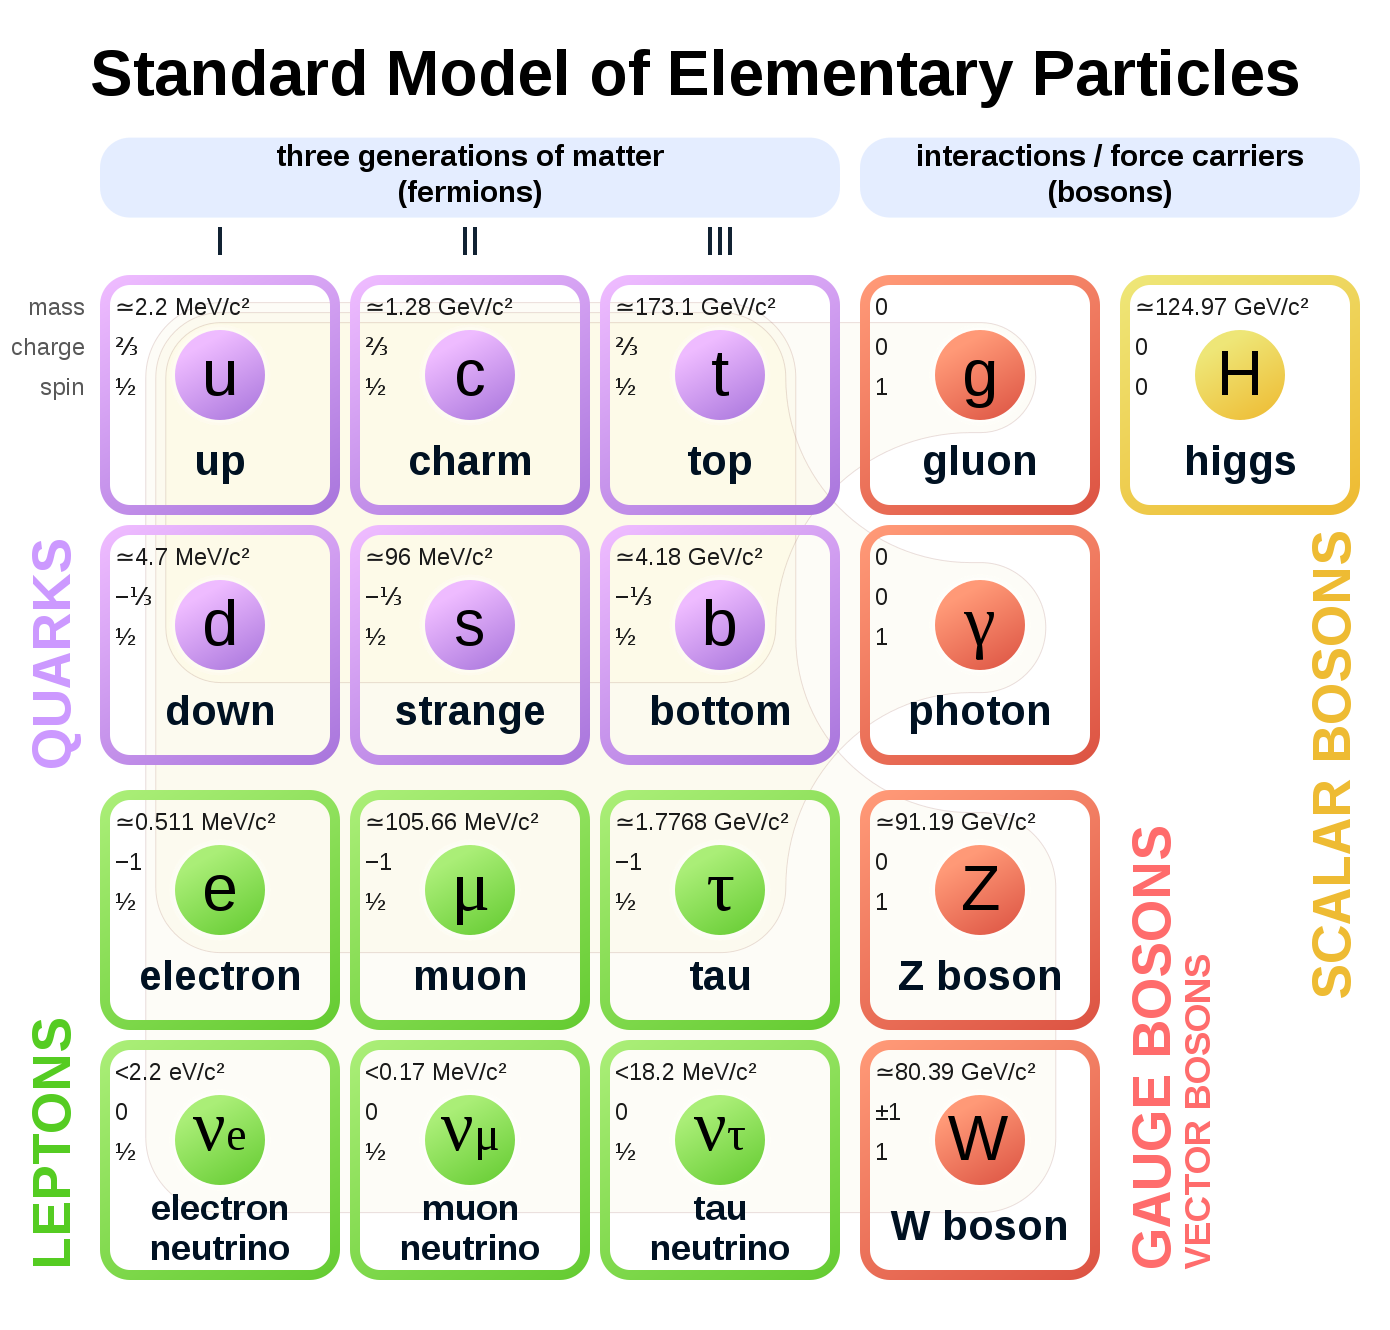
\includegraphics[width=0.75\textwidth]{fig/SM_particles.png}
 \caption{标准模型基本粒子总结。}
 \label{fig:SM_particles}
\end{figure}

标准模型是基于$SU(3)_C\bigotimes SU(2)_L\bigotimes U(1)_Y$群的规范场论,总共包含12个生成元。
每个生成元对应传递相互作用的一个规范玻色子,其中八个是胶子,为对称群为$SU(3)_C$的强相互作用传播子;
另外四个是$\gamma, W^{\pm}, Z$,为对称群为$SU(2)_L\bigotimes U(1)_Y$的电弱相互作用传播子。
为了保持规范对称性,这些中间传播子应当是无质量的。
夸克间的强相互作用由量子色动力学(QCD)描述,它具有渐近自由和夸克禁闭的性质。
电磁和弱作用由电弱统一理论(EW)描述,其中电磁相互作用通过光子传递,弱作用通过$W^{\pm}, Z$传递。
每种相互作用有不同的力程和强度,总结如表\ref{tab:summary_interactions}所示\footnote{弱相互作用常数具有GeV$^{-2}$量纲,为方便比较,乘上质子质量平方,引力作用常数也使用质子质量。} 。
弱作用的短力程和长作用时间表明中间玻色子($W^{\pm}, Z$)是有质量的,而这与规范对称性矛盾。
\begin{table}[h]
\centering
\begin{tabular}{c|c|c|c|c}
\hline
     		&强相互作用   &电磁相互作用  &弱相互作用 &引力相互作用 \\
\hline
源		&色荷  &电荷   &弱超荷   &质量 \\
相互作用常数 &$1\sim 10$  &$\approx$1/137   &$\approx 1\times 10^{-5}$    &$5\times 10^{-40}$ \\
力的传递者 &胶子  &光子  &$W^{\pm}, Z$  &- \\
典型作用时间(s) &$10^{-23}$  &$10^{-16}$  &$10^{-10}$   &- \\
力程  &1 fm  &$\infty$   &1/400 fm  &$\infty$  \\
\hline
\end{tabular}
\caption{四种相互作用特征表。}
\label{tab:summary_interactions}
\end{table}

希格斯机制\cite{PhysRevLett.13.321,HIGGS1964132,PhysRevLett.13.508,PhysRevLett.13.585,PhysRev.145.1156,PhysRev.155.1554}保持了理论的规范对称性,同时通过自发对称性破缺使得中间玻色子获得了质量,并且预言了一个新的标量粒子,即希格斯粒子。
经过几十年的寻找,希格斯粒子于2012年在LHC发现\cite{Aad:2012tfa,Chatrchyan:2012xdj}。虽然截止目前对希格斯粒子的测量并未发现明显超出标准模型迹象,但是误差较大。
精确测量希格斯粒子性质是非常重要的,因为任何的偏差会给新物理寻提供线索。顶夸克的汤川耦合是希格斯粒子测量的重要目标,顶夸克在标准模型中具有最大的质量,
理论表明它与希格斯粒子的汤川耦合是最强的,所以实验与理论的偏差有可能是新物理的迹象。
希格斯粒子关联顶夸克对产生模式($t\bar{t}h$)是这一测量的黄金过程,虽然$t\bar{t}h$产生截面只占希格斯粒子总产生截面的1\%,但是\RunTwo 是\RunOne 的几乎四倍,
为寻找$t\bar{t}h$提供了可能。

与夸克和轻子不同,希格斯粒子具有一独特的性质,即自耦合,自耦合常数的测量可以帮助验证和更深一步理解希格斯机制。
通过测量希格斯粒子对的产生可以帮助限制自耦合常数范围。
而且在许多新物理模型中,通过修改自耦合常数或者增加一个希格斯二重态可以增大希格斯粒子对的产生截面,
所以对希格斯粒子对的寻找也能帮助寻找新物理。

标准模型希格斯粒子多种衰变渠道,主要到$b\bar{b}$, $ZZ$, $\tau\tau$等。$h\rightarrow b\bar{b}$虽然有最高的分支比(58\%),但是在强子对撞机容易淹没在海量的喷注本底中。
而$h\rightarrow WW/\tau\tau$可为希格斯粒子提供标记,得益于它们的轻子末态或者强子化衰变的$\tau_{\text{had}}$。本文将论述通过多轻子道寻找$t\bar{t}h$和希格斯粒子对,结构如下:
第\ref{chap:higgs_pheno}章简要介绍希格斯唯象学,包括LHC单希格斯粒子产生,双希格斯粒子产生以及类希格斯对产生;
第\ref{chap:lhc_atlas}章首先描述LHC和ATLAS探测器,随后介绍ATLAS实验事例重建,事例仿真等过程,最后介绍ATLAS Phase-II升级以及
硅微条探测器模块组装和测试;
第\ref{chap:tth_multilep}章论述通过多轻子道寻找$t\bar{t}h$产生,主要关注由单轻子和两$\tau_{\text{had}}$的组成的信号道的数据分析过程,并给出统计结果;
第\ref{chap:hh_serach}章展示通过多轻子道寻找希格斯粒子对和类希格斯对产生,重点论述相同电荷双轻子分析道,最后给出统计结果;
第\ref{chap:conclusions}章作出文章总结,并对未来的分析工作作出一定展望。

%\part{粒子物理实验理论}
\chapter{希格斯唯象学}\label{chap:higgs_pheno}
\chapter{一些准备}
%在粒子物理领域,主要实验工具是对撞机,并分为环形和直线,直线对撞机的质心系能量受限于加速电压和直线距离,并且没有储存环,亮度不会太高。
%所以,环形对撞机是能量前沿新物理寻找的理想工具。加速粒子种类主要有电子和质子\footnote{因为本文关注质子对撞物理,暂且不表打靶实验和其他形式对撞实验},因为电子比质子具有更强
%的同步辐射,对于同样大小的储存环,很难加速到同一能量,
质子对撞可以产生丰富的物理过程,这得益于质子是一个复合粒子。对于一定能量(GeV以上)的质子,在每次对撞中,
往往是质子的某一部分(Parton,部分子)参与相互作用(图\ref{fig:pp_collision}),
而这一部分的能量是不确定的,多种多样具有不同能量阈值的物理过程才可以发生。
但是为了准确预测各种物理过程的产生截面,我们需要了解质子中各部分子的能量分布情况。
通过深度非弹实验\cite{Kuhlen:390284},单举喷注产生\cite{Aad2015-pdf}或者强子对撞机的电弱过程测量\cite{Khachatryan2016,Khachatryan2015},我们可以得知具有特定比例动量$x$的部分子的存在概率$f(x)$,即PDF(Parton Distribution Function)。
但是是这些测量均在特定$\mu$(代表散射过程中的典型能量转移大小)进行,得到的PDF须根据微扰QCD演化公式\cite{ellis_stirling_webber_1996}外推到LHC能量尺度。
图\ref{fig:NNPDF3}展示LHC常用的一种PDF,
值得指出的是,$\mu^2=10^4~\text{GeV}^2$表示希格斯粒子产生过程的典型能量转移,在13 TeV质心系能量下,$x$大约为$10^{-2}$,所以LHC希格斯粒子产生的主要贡献来自胶子融合。
\begin{figure}[h]
\centering
 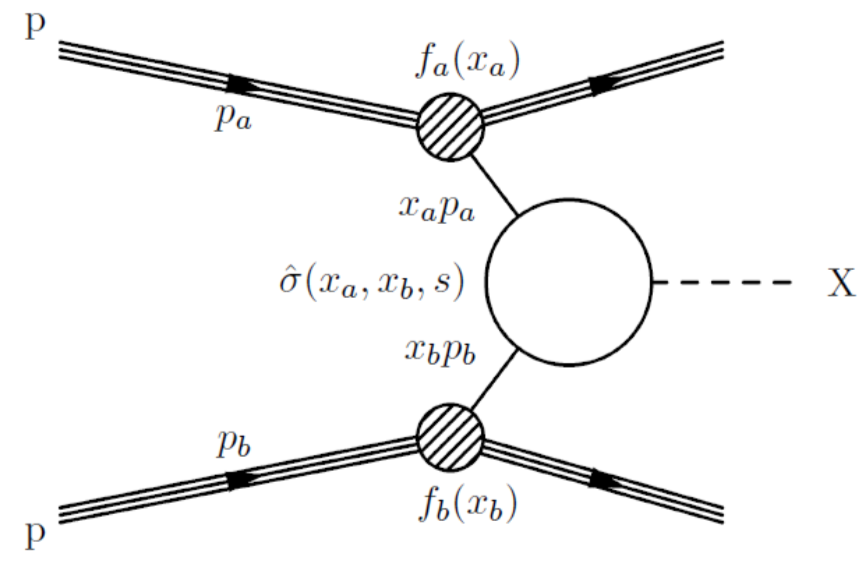
\includegraphics[width=0.75\textwidth]{fig/inclusive_pp.png}
 \caption{质子-质子对撞中的部分子硬散射过程。}
 \label{fig:pp_collision}
\end{figure}
\begin{figure}[h]
\centering
 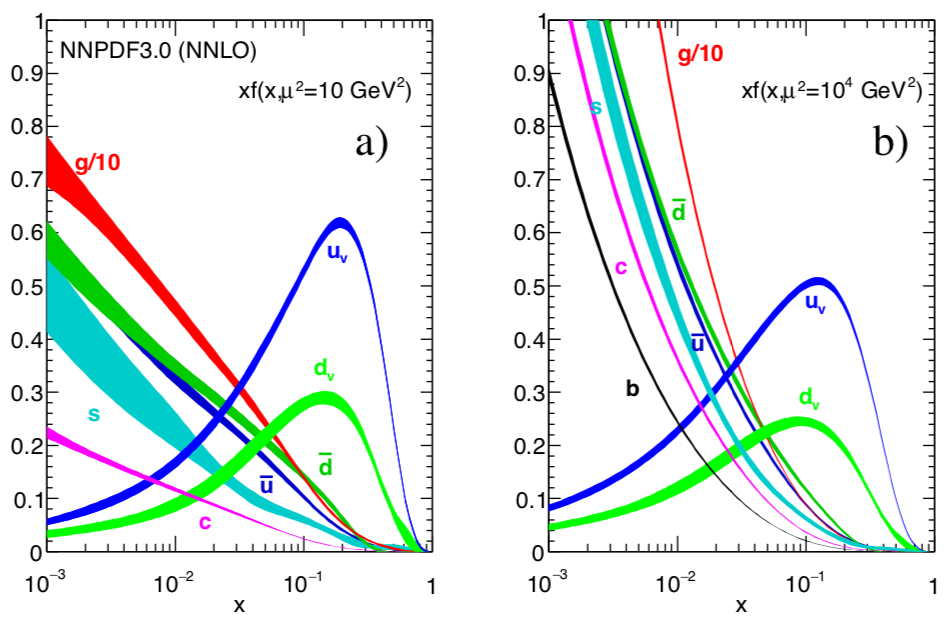
\includegraphics[width=0.75\textwidth]{fig/NNPDF3.png}
 \caption{NNPDF3.0\cite{24}在$\mu^2=10~\text{GeV}^2$和$\mu^2=10^4~\text{GeV}^2$时的质子部分子分布函数$xf(x)$,其中曲线宽度代表PDF误差。}
 \label{fig:NNPDF3}
\end{figure}
之后,根据因子化定理\cite{Collins:1989gx},图\ref{fig:pp_collision}所示的质子-质子对撞的单举产生截面则为:
\begin{equation}
 \sigma_{pp\rightarrow X}=\sum_{a,b}\int dx_adx_bf_a(x_a,\mu_F^2)f_b(x_b,\mu_F^2)\hat{\sigma}_{ab\rightarrow X}(x_ap_a,x_bp_b,\mu_R^2,\mu_F^2)
\end{equation}
其中对所有可以发生某过程的各种味道部分子求和,部分子的PDF$f_i(x_i,\mu_F^2)$依赖$\mu_F^2$,即因子化尺度,代表探查质子时的能量尺度,
而硬散射过程$ab\rightarrow X$截面还依赖于QCD重整化大小$\mu_R^2$。需要指出的是,$\mu_F$和$\mu_R$都是为了计算结果有物理意义而人为选择的参数,
在微扰QCD中,如果能够计算散射过程的所有展开阶数,物理过程的产生截面不依赖于$\mu_F$和$\mu_R$,
但是在有限阶数的计算下,$\mu_F$和$\mu_R$的大小选择会影响截面的计算结果,这也是理论误差的来源之一。
\section{希格斯物理}
标准模型引入了一个具有非零真空期望值的复标量Higgs场,$\varphi$,其场势能项为:
\begin{equation}
 V(\varphi)=-v^2\lambda\varphi^{\dagger}\varphi+\lambda(\varphi^{\dagger}\varphi)^2
\end{equation}
其中,$v=(\sqrt{2}G_{F})^{-1/2}\approx246~$GeV为Higgs场真空期望值,$\lambda$是Higgs自耦合参数。通过自发对称性破缺,$W^{\pm}$和$Z$玻色子得到质量,
而且预言了一个额外的标量粒子,即Higgs玻色子。在标准模型中包含Higgs耦合项的拉氏量密度如公式\ref{eq:Higgs_Lagrangian}所示:
\begin{equation}
\label{eq:Higgs_Lagrangian}
\mathcal{L}=-\lambda\bar{f}fh+\delta_{V}V_{\mu}V^{\mu}(\lambda_{hVV}h+\lambda_{hhVV}h^2)+\lambda_{hh}h^2+\lambda_{hhh}h^3+\lambda_{hhhh}h^4
\end{equation}
其中,$f$代表费米子,$V$为$W^{\pm}$($\delta_{W}$=1)和$Z$($\delta_{Z}$=1/2)玻色子,并且方程中的耦合参数可以表达为:
\begin{equation}
 \begin{aligned}
 \lambda_{h\bar{f}f}=\frac{m_{f}}{v},~\lambda_{hVV}=\frac{2m_{V}^{2}}{v},~\lambda_{hhVV}=\frac{m_{V}^2}{v^2} \\
 \lambda_{hh}=\frac{m_{h}^2}{2},~\lambda_{hhh}=\frac{m_{h}^2}{2v}=\lambda v,~\lambda_{hhhh}=\frac{m_{h}^2}{8v^2}
 \end{aligned}
\end{equation}
Higgs质量模型并未预言,需要实验确定,当Higgs粒子质量确定之后,Higgs自耦合参数$\lambda_{hhh}$也随之确定,$\lambda_{hhh}$的测量是$hh$搜寻的首要目标。
还可以发现,Higgs与其他粒子的耦合强度与粒子质量成正比。

\subsection{单希格斯粒子产生模式}
在LHC单希格斯粒子可以有以下产生模式:
\begin{itemize}
 \item 胶子融合(ggF): $gg\rightarrow h$;
 \item 矢量玻色子融合(VBF): $q\prime{q}\rightarrow q\prime{q}h$;
 \item $W$或$Z$玻色子关联产生(Vh): $q\bar{q}\rightarrow Vh$,其中还包括部分($\sim$8\%): $gg\rightarrow Zh$(ggZh);
 \item 底夸克对关联产生($b\bar{b}h$): $q\bar{q}/gg\rightarrow b\bar{b}h$,和顶夸克对关联产生($t\bar{t}h$): $q\bar{q}/gg\rightarrow t\bar{t}h$;
 \item $t$过程单顶夸克关联产生($thqb$): $qg\rightarrow th\prime{q}b$(四味方案),和关联$W$玻色子产生($thW$): $gb\rightarrow thW$(五味方案), $s$过程可以忽略。
\end{itemize}
图\ref{fig:LHCHIGGSWG}分别总结了上述几种产生模式在$\sqrt{s}=13~$TeV时产生截面随$m_h$变化情况,和在$m_h$=125 GeV时随$\sqrt{s}$变化情况。
\begin{figure}[h]
\centering
 \begin{subfigure}[b]{0.45\textwidth}
  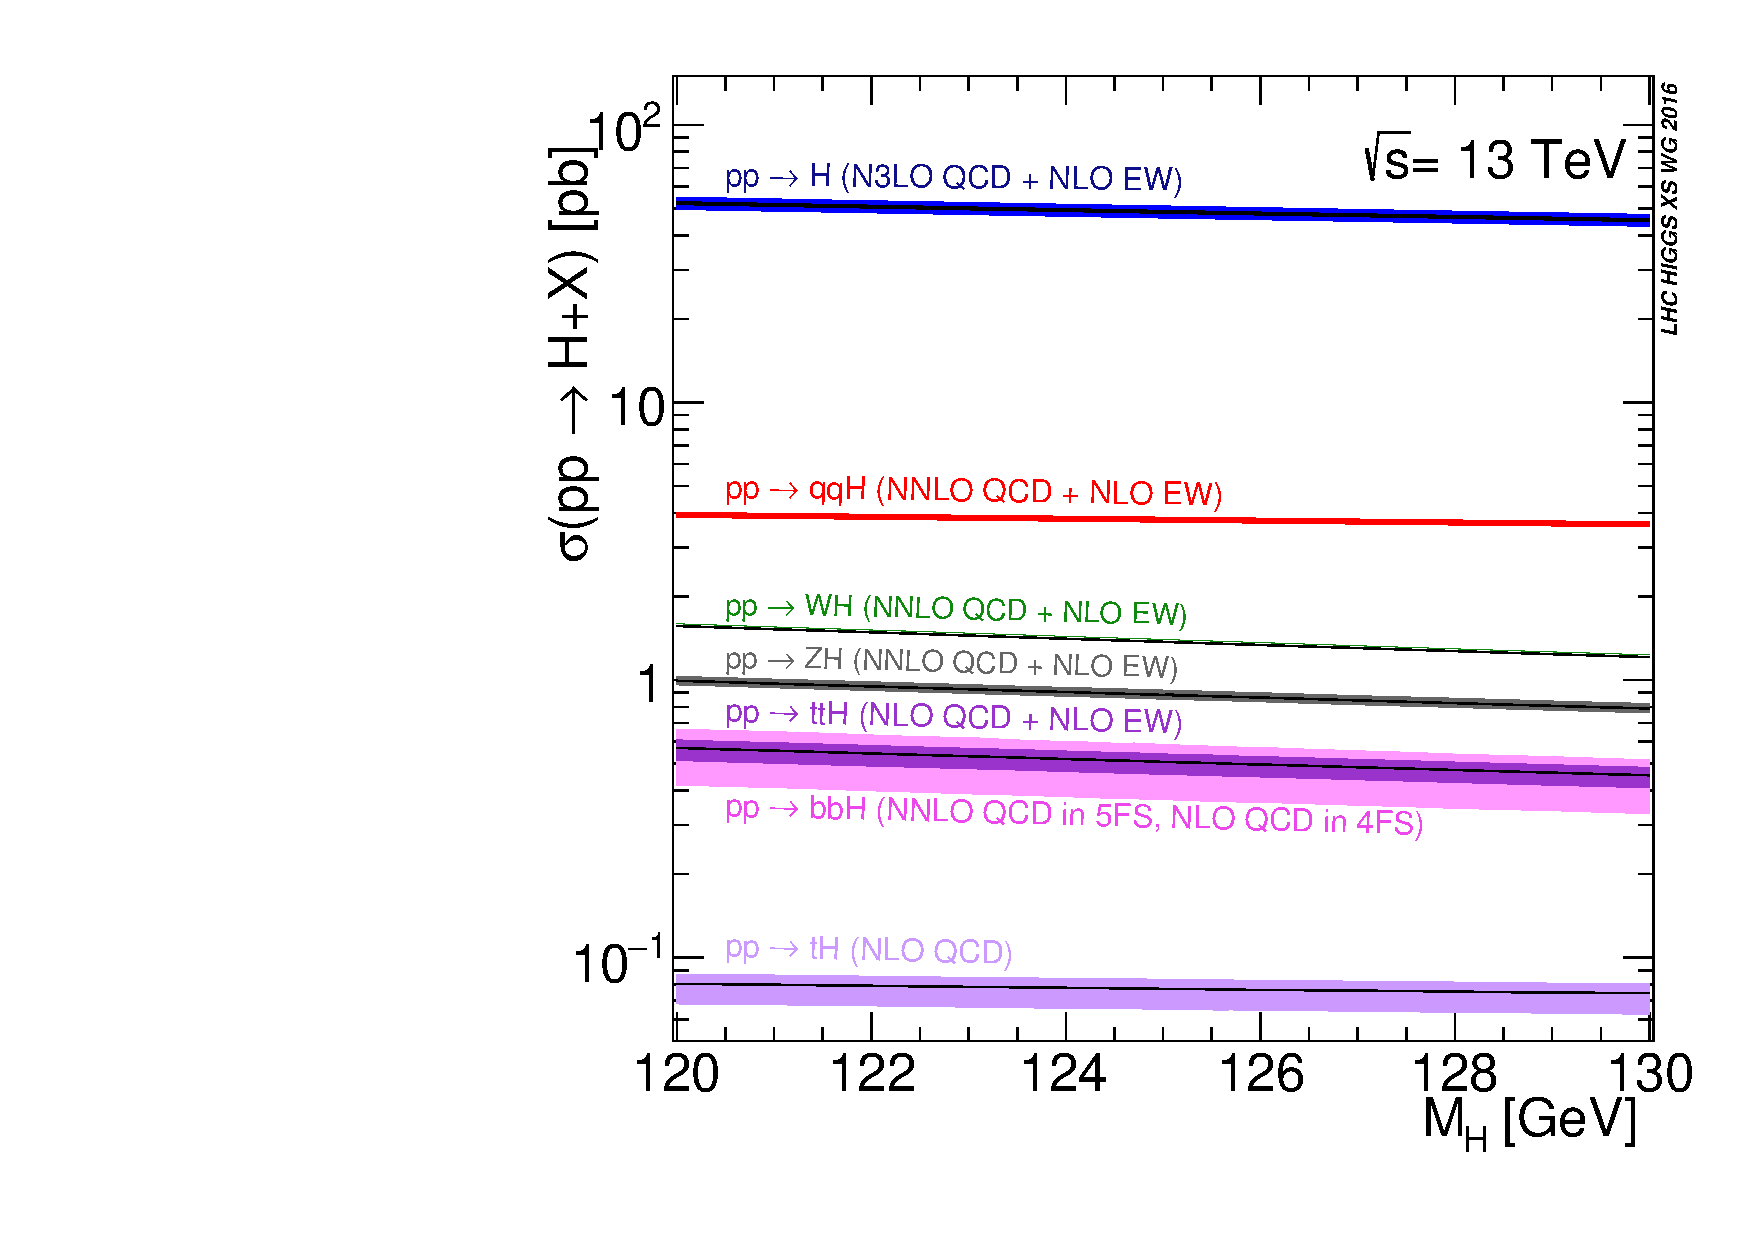
\includegraphics[width=0.75\textwidth,angle=-90]{fig/plot_13tev_H_sqrt.pdf}
  \caption{}
 \end{subfigure}
 \begin{subfigure}[b]{0.45\textwidth}
  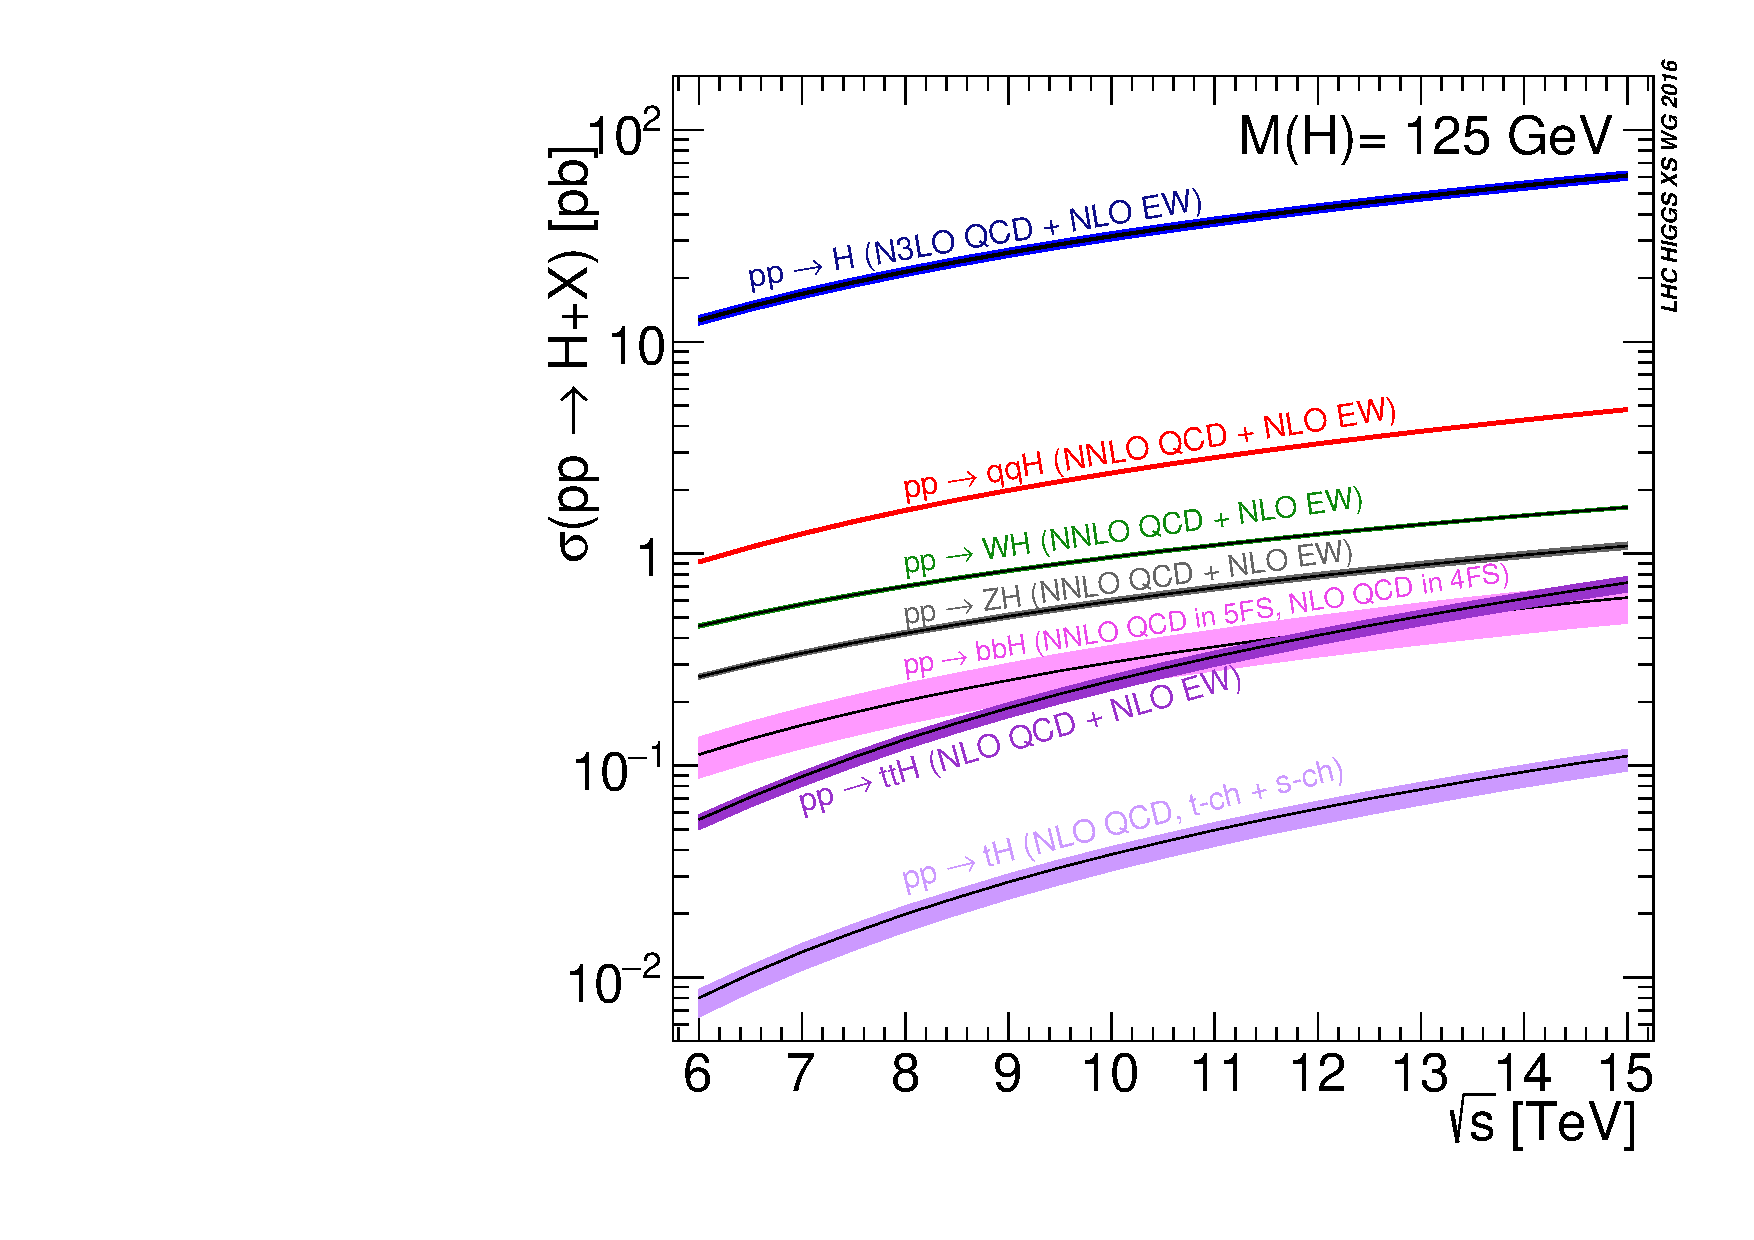
\includegraphics[width=0.75\textwidth,angle=-90]{fig/Plot_Escan_H125_new_sqrt.pdf}
  \caption{}
 \end{subfigure}
\caption{(a)标准模型希格斯粒子各产生模式截面随$m_h$变化($\sqrt{s}=13~$TeV),(b)标准模型希格斯粒子各产生模式截面随$\sqrt{s}$变化($m_h=125~$GeV)。}
\label{fig:LHCHIGGSWG}
\end{figure}
$ggF$是LHC上Higgs产生的主要过程,大约占比90\%($m_h$=125 GeV),是Higgs发现的首要贡献过程。在一般的超出标准模型设置中,$ggF$也假设为主要贡献过程,如本文将要
研究的$hh$产生。不过需要指出的是,$ggF$这过程有很高的QCD本底,不能很好地纯化。图\ref{fig:diagram_ggF}是$ggF$的领头阶(LO)的费曼图,因为胶子是无质量的,所以必须通过重味夸克传递。\\
$VBF$具有第二大的产生截面,其LO的费曼图如图\ref{fig:diagram_VBF}所示,除了产生Higgs外,还有两个较前向的喷注,这是它的显著信号特征,可以与$ggF$进行很好区分;
$VBF$于2018年被正式发现\cite{ATLAS:2018doi}。
\begin{figure}[h]
\centering
 \begin{subfigure}[b]{0.45\textwidth}
  %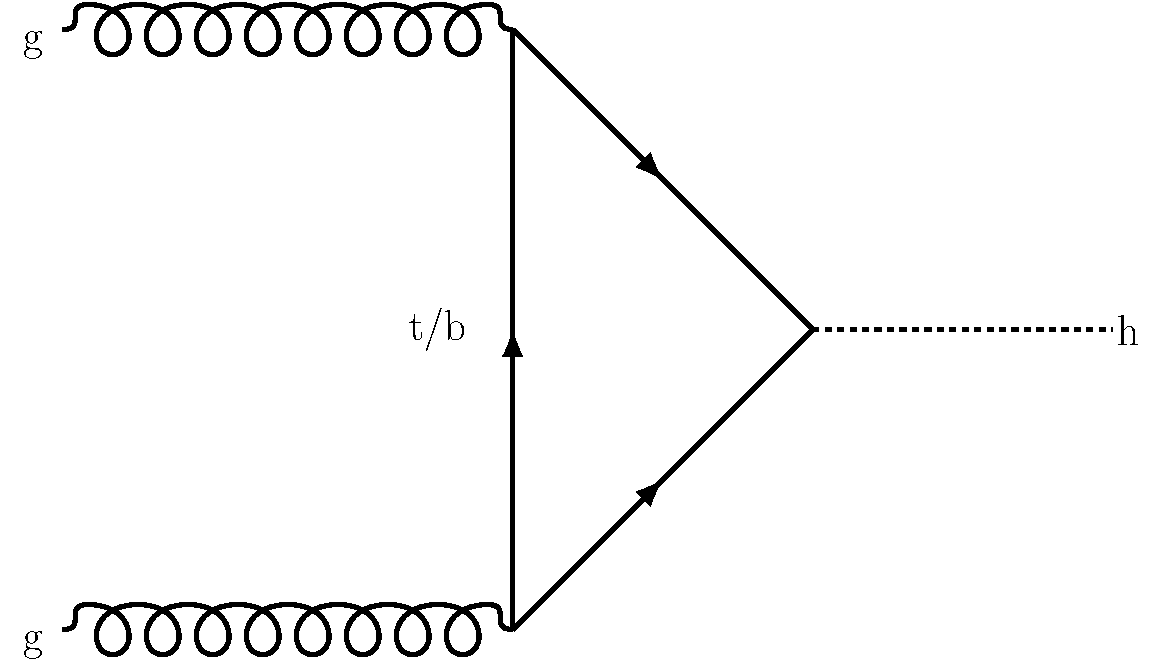
\includegraphics[width=0.75\textwidth]{fig/ggF.pdf}
  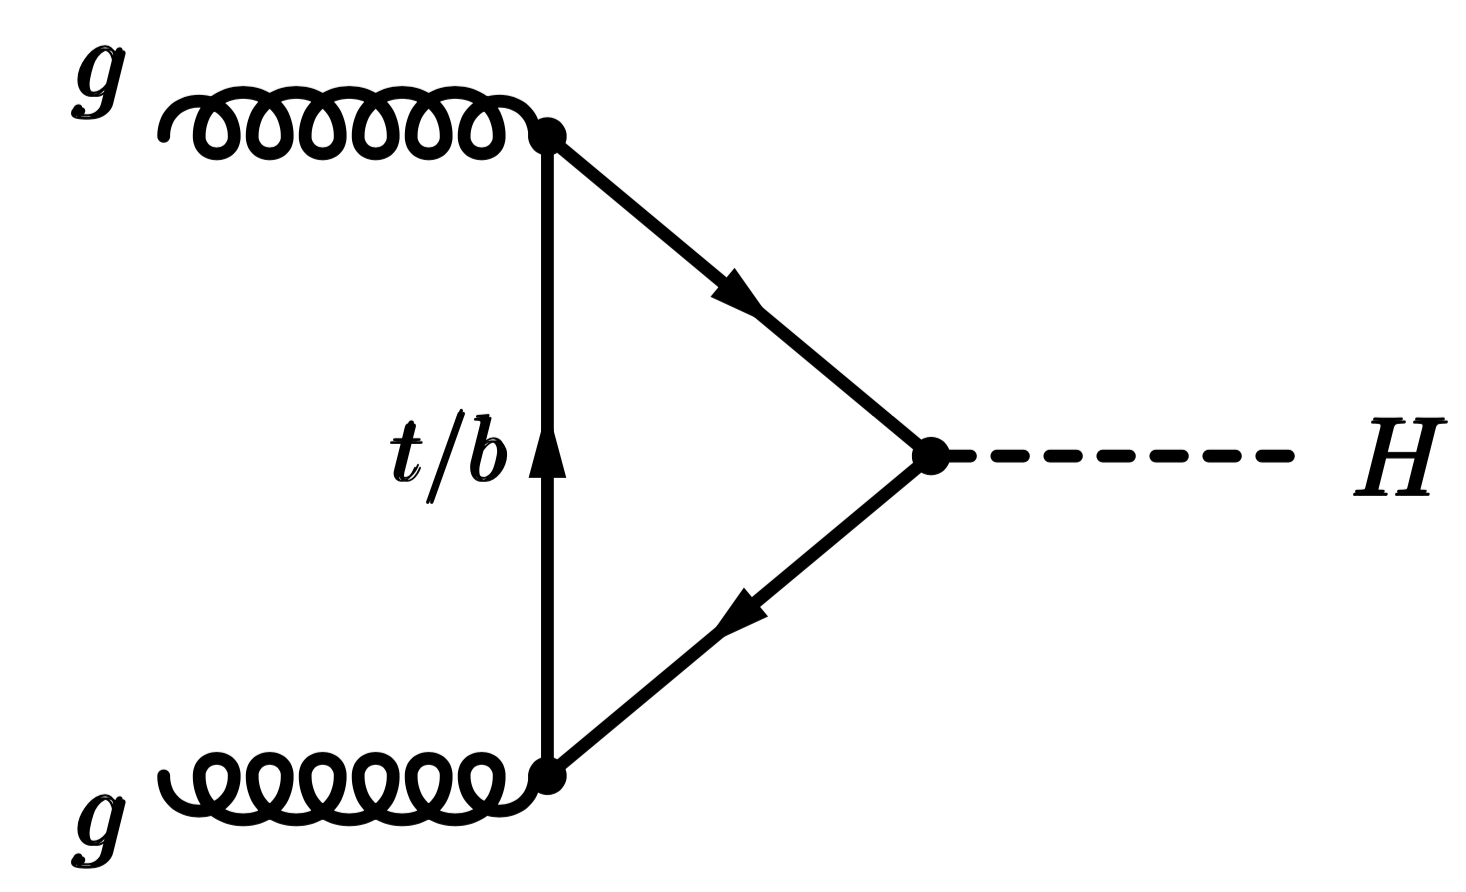
\includegraphics[width=0.75\textwidth]{fig/diagram_ggF.png}
  \caption{}
  \label{fig:diagram_ggF}
 \end{subfigure}
 \begin{subfigure}[b]{0.45\textwidth}
  %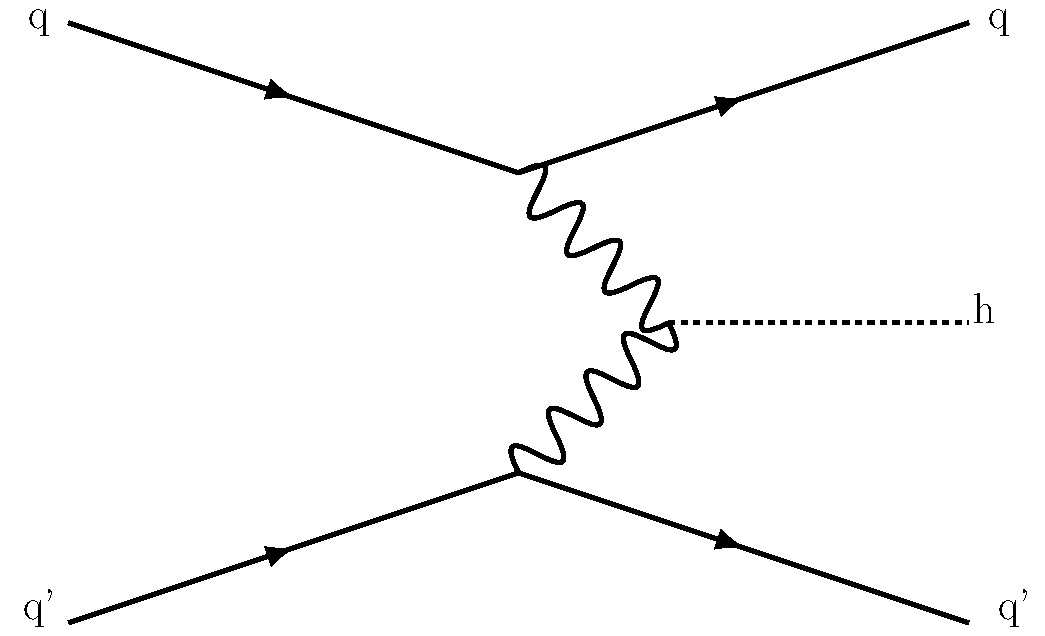
\includegraphics[width=0.75\textwidth]{fig/VBF.pdf}
  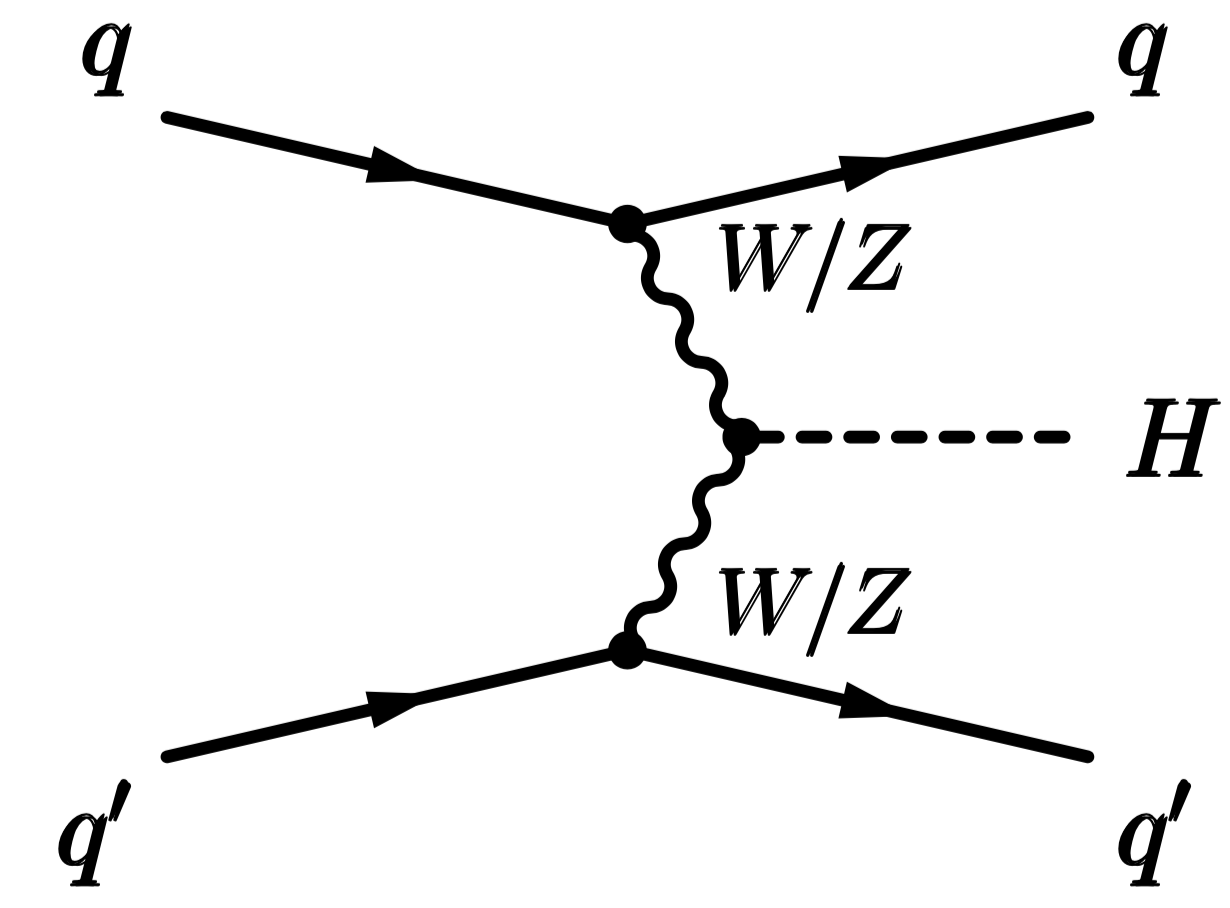
\includegraphics[width=0.75\textwidth]{fig/diagram_VBF.png}
  \caption{}
  \label{fig:diagram_VBF}
 \end{subfigure}
\caption{(a)LO阶$ggF$产生过程;(b)LO阶$VBF$产生过程。}
\label{fig:ggF_VBF}
\end{figure}
$Vh$过程的显著特征是末态中只有一个$W$或$Z$玻色子和Higgs,其LO阶费曼图如图\ref{fig:diagram_VH}所示。它可以通过玻色子的轻子化衰变产物去寻找,从而极大地压低QCD本底。
$Vh$是发现$h\rightarrow b\bar{b}$的黄金过程,并已于2018年正式发现\cite{Aaboud:2018zhk,Sirunyan:2018kst}。
通过$Vh$过程,我们还可以测量$\lambda_{hVV}$参数。另外,$ggZh$的产生截面很小,一般在的Higgs性质测量中,没有考虑。\\
\begin{figure}[h]
\centering
 \begin{subfigure}[b]{0.33\textwidth}
  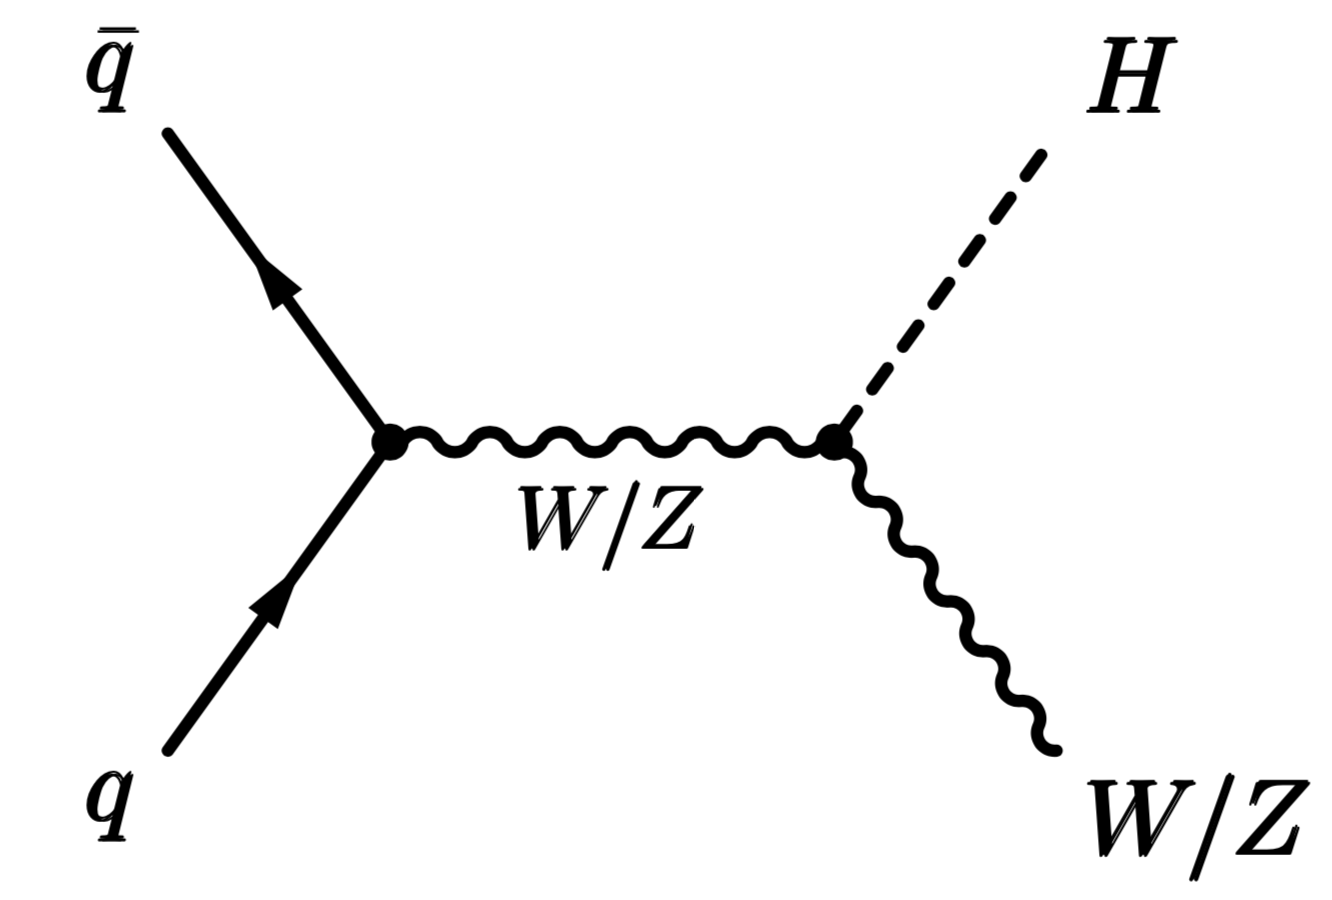
\includegraphics[width=0.85\textwidth]{fig/diagram_VH.png}
  \caption{}
  \label{fig:diagram_VH}
 \end{subfigure}
 \begin{subfigure}[b]{0.33\textwidth}
  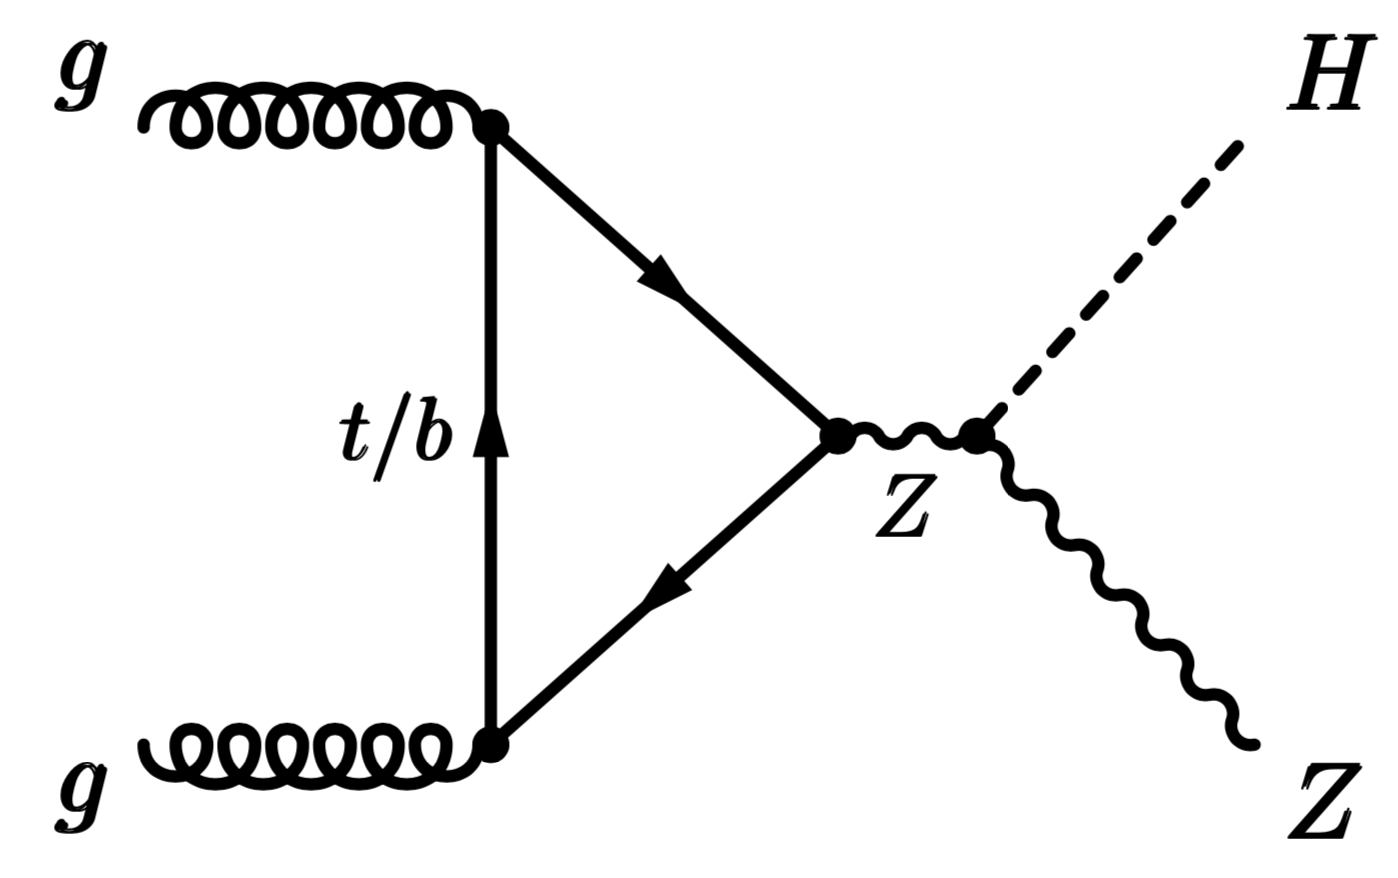
\includegraphics[width=0.85\textwidth]{fig/diagram_ggZh1.png}
  \caption{}
  \label{fig:diagram_ggzh1}
 \end{subfigure}
 \begin{subfigure}[b]{0.33\textwidth}
  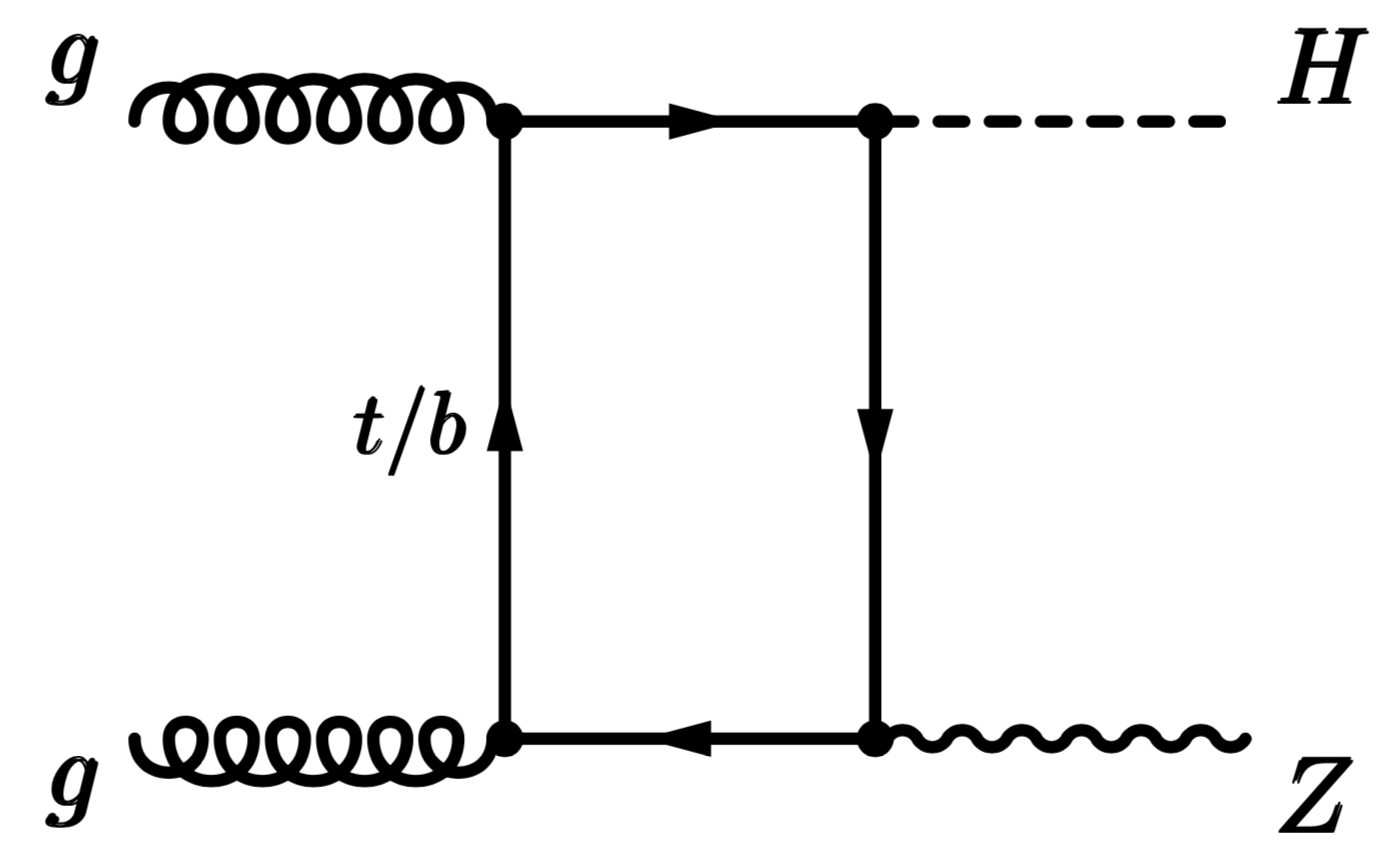
\includegraphics[width=0.85\textwidth]{fig/diagram_ggZh2.png}
  \caption{}
  \label{fig:diagram_ggzh1}
 \end{subfigure}
\caption{(a)LO阶$Vh$产生过程;(b)(c)LO阶$ggZh$产生过程。}
\label{fig:Vh_ggZh}
\end{figure}

相比于$ggF$和$VBF$,$b\bar{b}h$和$t\bar{t}h$产生截面很小。对于$b\bar{b}h$,其挑战在于一般$b$夸克动量很低,不能有效地标记。而对于$t\bar{t}h$,得益于顶夸克的质量,
其衰变产物,如$b$喷注,具有较高的动量,可以有效标记,最终可以标记到此过程的相空间。通过$t\bar{t}h$的研究可以测量Higgs与最重粒子的Yukawa耦合参数。
在ATLAS,$t\bar{t}h$是近几年的研究热点,已开展$t\bar{t}h(\rightarrow\gamma\gamma)$,$t\bar{t}h(\rightarrow b\bar{b})$以及$t\bar{t}h(\rightarrow \ell/\tau)$(一般称为tthML),
其中tthML研究将在本文讲述。$t\bar{t}h$的LO费曼图见图\ref{fig:diagram_tth}。\\
\begin{figure}[h]
\centering
 \begin{subfigure}[b]{0.33\textwidth}
  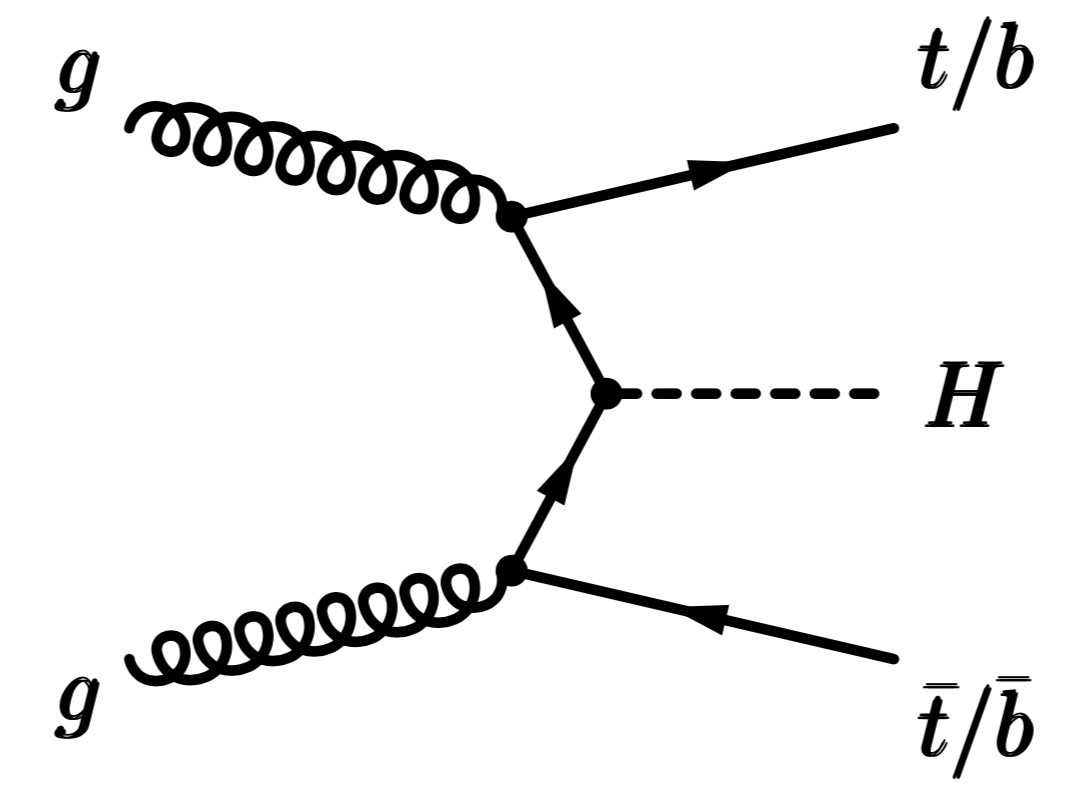
\includegraphics[width=0.85\textwidth]{fig/diagram_tth1_LO.png}
  \caption{}
 \end{subfigure}
 \begin{subfigure}[b]{0.33\textwidth}
  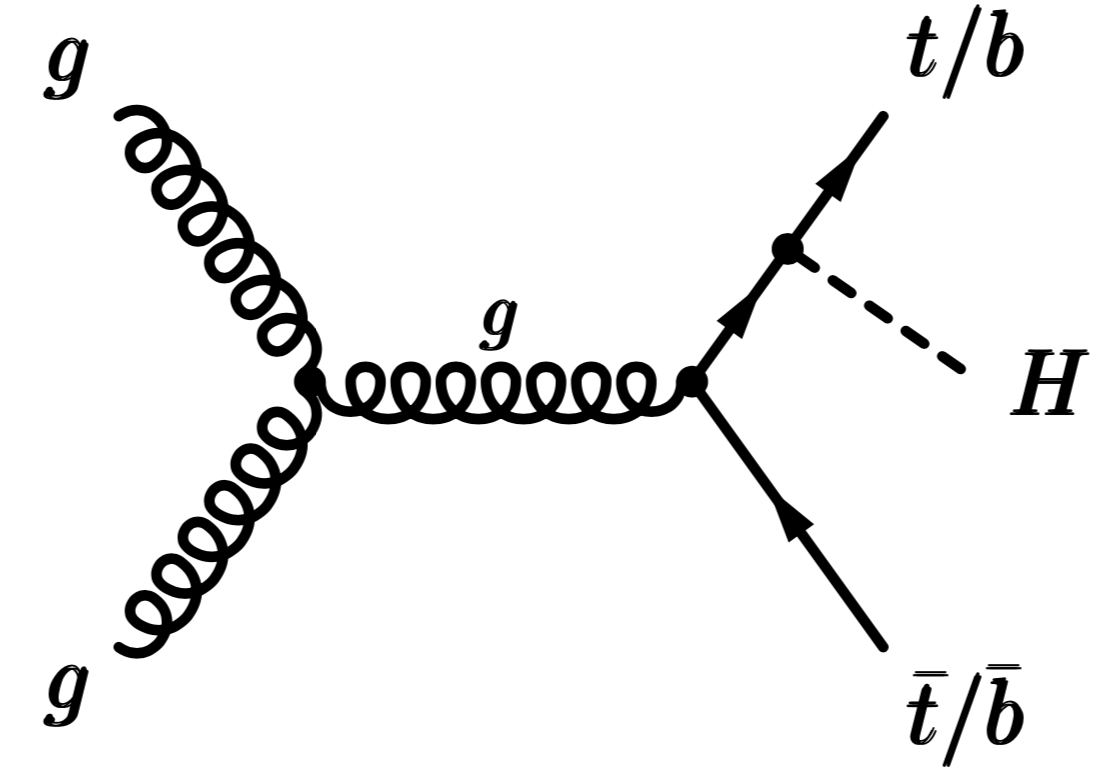
\includegraphics[width=0.85\textwidth]{fig/diagram_tth2_LO.png}
  \caption{}
 \end{subfigure}
 \begin{subfigure}[b]{0.33\textwidth}
  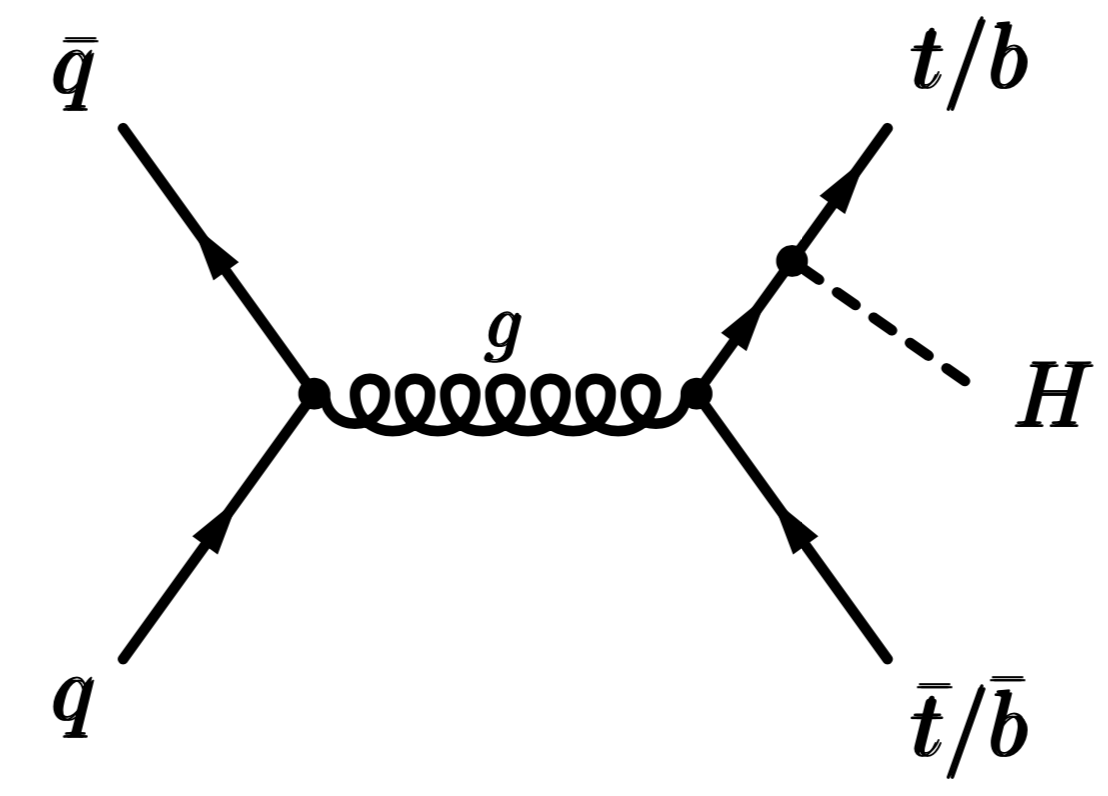
\includegraphics[width=0.85\textwidth]{fig/diagram_tth3_LO.png}
  \caption{}
 \end{subfigure}
\caption{LO阶$t\bar{t}h$和$b\bar{b}h$费曼图。}
\label{fig:diagram_tth}
\end{figure}

$th$过程,具有最小的产生截面,其LO阶费曼图如图\ref{fig:diagram_th}所示。它的末态产物跟$t\bar{t}h$很相似,可以跟$t\bar{t}h$一起研究,联合测量Higgs与顶夸克的Yukawa耦合常数。\\
\begin{figure}[h]
\centering
 \begin{subfigure}[b]{0.33\textwidth}
  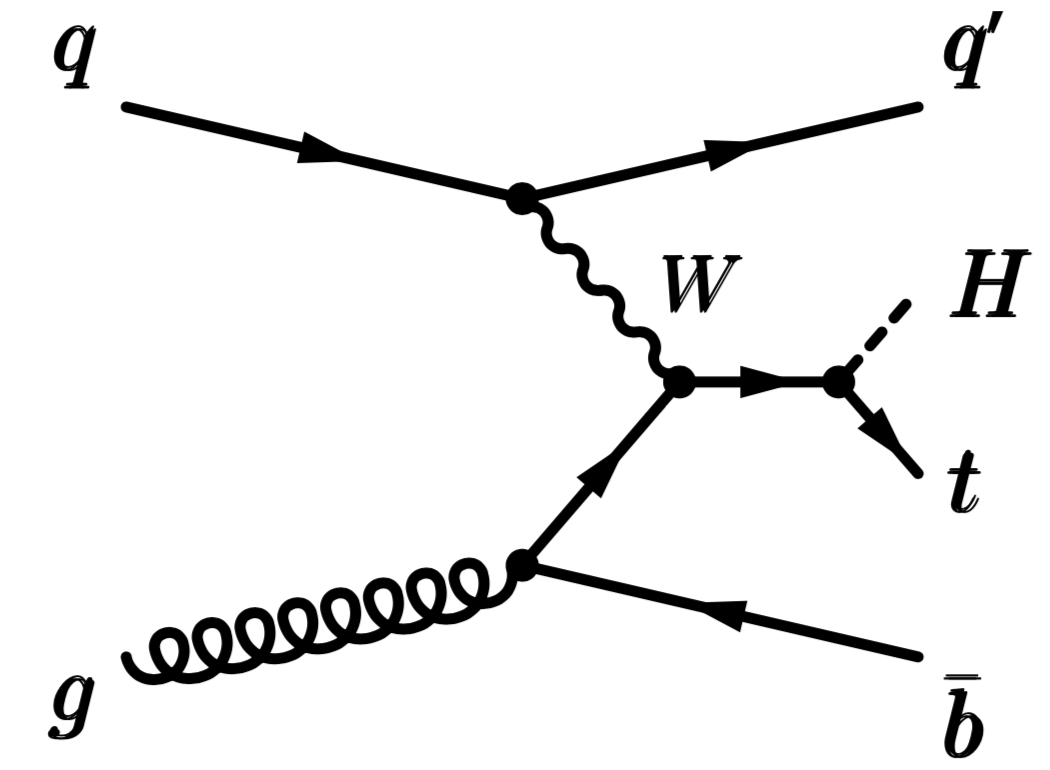
\includegraphics[width=0.85\textwidth]{fig/diagram_thqb1.png}
  \caption{}
  \label{fig:diagram_VH}
 \end{subfigure}
 \begin{subfigure}[b]{0.33\textwidth}
  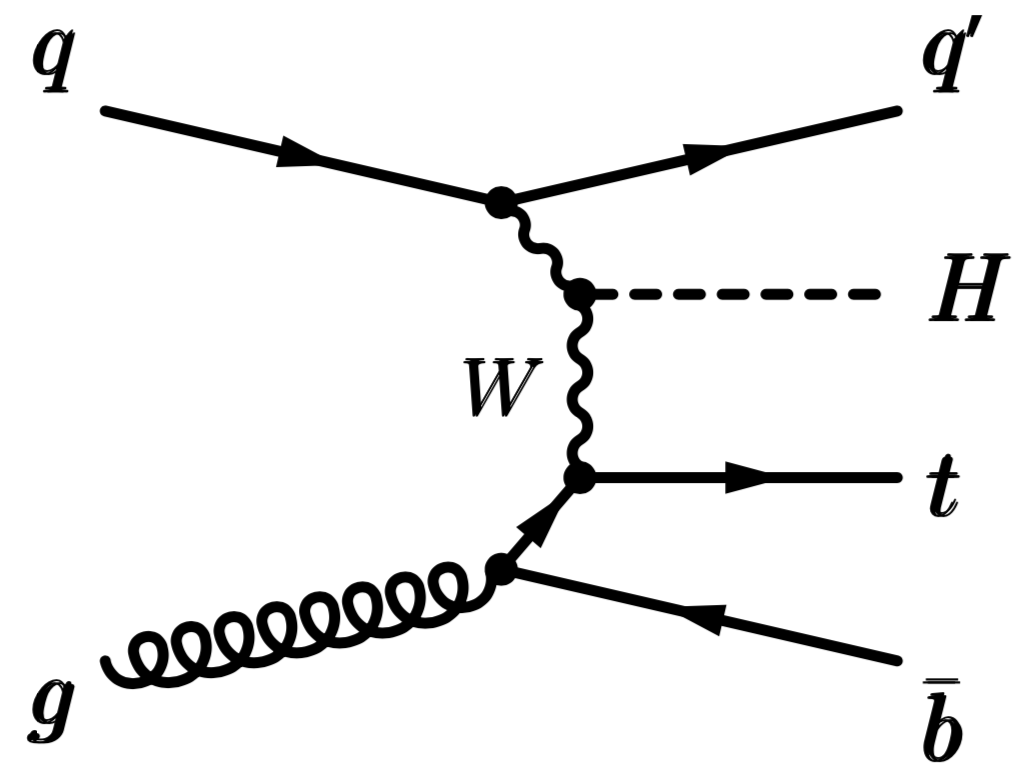
\includegraphics[width=0.85\textwidth]{fig/diagram_thqb2.png}
  \caption{}
  \label{fig:diagram_ggzh1}
 \end{subfigure}
 \begin{subfigure}[b]{0.33\textwidth}
  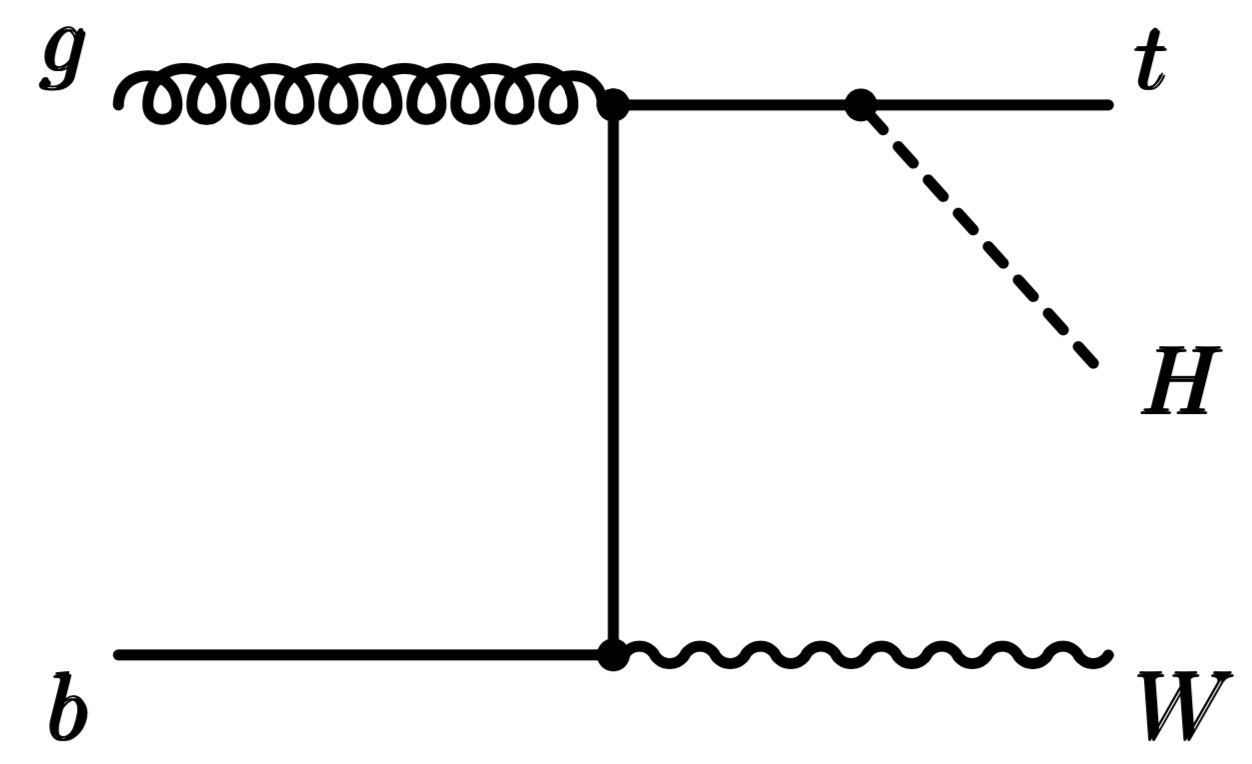
\includegraphics[width=0.85\textwidth]{fig/diagram_thW1.png}
  \caption{}
  \label{fig:diagram_ggzh1}
 \end{subfigure}
 \begin{subfigure}[b]{0.33\textwidth}
  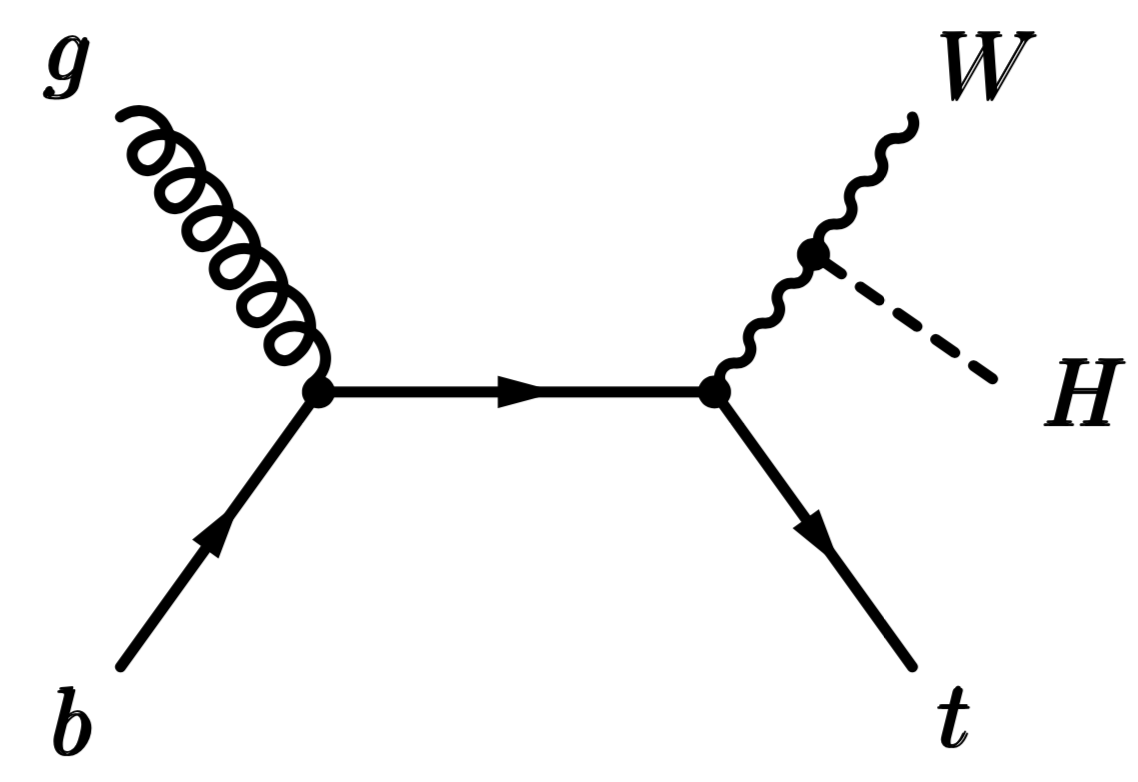
\includegraphics[width=0.85\textwidth]{fig/diagram_thW2.png}
  \caption{}
  \label{fig:diagram_ggzh1}
 \end{subfigure}
\caption{(a)(b)典型LO阶$thqb$过程;(c)(d)典型LO阶$thW$过程。}
\label{fig:diagram_th}
\end{figure}

表\ref{tab:xs_single_higgss_prod}总结这些产生过程在$\sqrt{s}=13~$TeV时的截面,其计算QCD阶数和QED阶数也列出。
\begin{table}[h]
\centering
\scalebox{0.75}{
\begin{tabular}{ccc}
\hline
\hline
Production porcess   &Cross section [pb]    &Order of calculation \\
\hline
$ggF$   &48.61+$(\text{theory})^{+4.27\%}_{-6.49\%}(\text{PDF})^{+1.85\%}_{-1.85\%}(\alpha_s)^{+2.59\%}_{-2.62\%}$   &N$^3$LO QCD + NLO EW  \cite{XSWG13TeV_2019,Cepeda:2019klc}\\
$VBF$   &3.766+$(\text{scale})^{+0.43\%}_{-0.33\%}(\text{PDF}+\alpha_s)^{+2.1\%}_{-2.1\%}$   &NNLO QCD +  NLO EW \cite{XSWG13TeV_2019,Cepeda:2019klc} \\
$Wh$   &1.358+$(\text{scale})^{+0.51\%}_{-0.51\%}(\text{PDF}+\alpha_s)^{+1.35\%}_{-1.35\%}$   &NNLO QCD + NLO EW \cite{XSWG13TeV_2019,Cepeda:2019klc}  \\
$Zh$   &0.880+$(\text{scale})^{+3.50\%}_{-2.68\%}(\text{PDF}+\alpha_s)^{+1.65\%}_{-1.65\%}$    &NNLO QCD + NLO EW \cite{XSWG13TeV_2019,Cepeda:2019klc} \\
%$ggZh $    &    &  \\
$t\bar{t}h$  &0.507+$(\text{scale})^{+5.8\%}_{-9.2\%}(\text{PDF}+\alpha_s)^{+3.6\%}_{-3.6\%}$    &NLO QCD + NLO EW \cite{XSWG13TeV} \\
%$th$  &    &NLO QCD  \\
$b\bar{b}h$  &0.486+$(\text{scale}+\text{PDF}+\alpha_s)^{+20.1\%}_{-23.9\%}$   &5FS NNLO + 4FS NLO \cite{XSWG13TeV} \\
$th$ &0.848+$(\text{scale+FS})^{+6.6\%}_{-13.3\%}(\text{PDF}+\alpha_s)^{+3.3\%}_{-3.3\%}$  &NLO QCD \cite{deFlorian:2016spz}\\      
%\hline
%Total    &    &  \\ 
\hline
\hline
\end{tabular}}
\caption{13 TeV质心系能量下标准模型希格斯玻色子(假设$m_h$= 125.09 GeV)产生截面理论预测值(pb),其中误差包括来自QCD scales, PDF以及$\alpha_s$的不确定度。}
\label{tab:xs_single_higgss_prod}
\end{table}

\subsection{标准模型希格斯对产生}
标准模型还预言了希格斯对产生,与单Higgs产生类似,其主要来源是胶子融合过程。在LHC LO阶的产生过程如图\ref{fig:diagram_SMhh_ggF}所示,分为箱图(\ref{fig:diagram_SMhh_box})和能够测量$\lambda_{hhh}$的三角图(\ref{fig:diagram_SMhh_triangle})。
在三角图中,中间态的Higgs作为一个传播子,质量不在壳,而末态的双Higgs均在壳;而中间态Higgs在壳,末态Higgs不在壳的情况被极大地压低\cite{Patrignani:2016xqp}\textbf{引用存疑}。
而且需要指出的是,箱图和三角图过程具有抵消干涉项,导致标准模型希格斯对总产生截面很小。
\begin{figure}[h]
\centering
 \begin{subfigure}[b]{0.45\textwidth}
  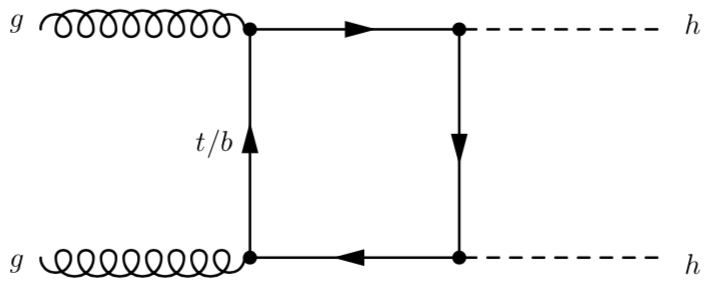
\includegraphics[width=0.85\textwidth]{fig/SMhh_box.png}
  \caption{}
  \label{fig:diagram_SMhh_box}
 \end{subfigure}
 \begin{subfigure}[b]{0.45\textwidth}
  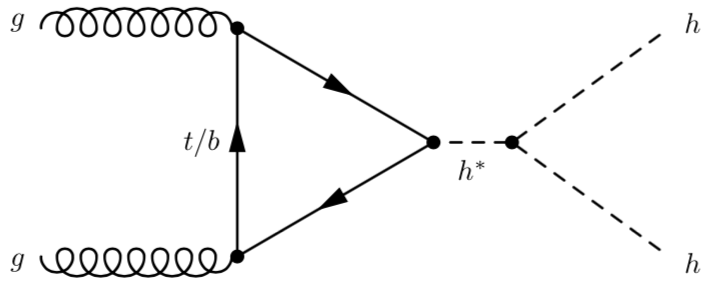
\includegraphics[width=0.85\textwidth]{fig/SMhh_triangle.png}
  \caption{}
  \label{fig:diagram_SMhh_triangle}
 \end{subfigure}
\caption{领头阶标准模型$hh$胶子融合产生过程。}
\label{fig:diagram_SMhh_ggF}
\end{figure}

另外,除了胶子融合过程,还有其他Higgs对产生模式,比如矢量玻色子融合,其领头阶费曼图如图\ref{fig:diagram_SMhh_VBF}所示。
需要指出的是,在ATLAS利用2015年和2016年数据进行的分析中,仅考虑了胶子融合过程,这也是本文$hh$研究的考虑范围。
%但是在新一轮的研究中,一些分析道开始考虑矢量玻色子融合过程。
\begin{figure}[h]
\centering
  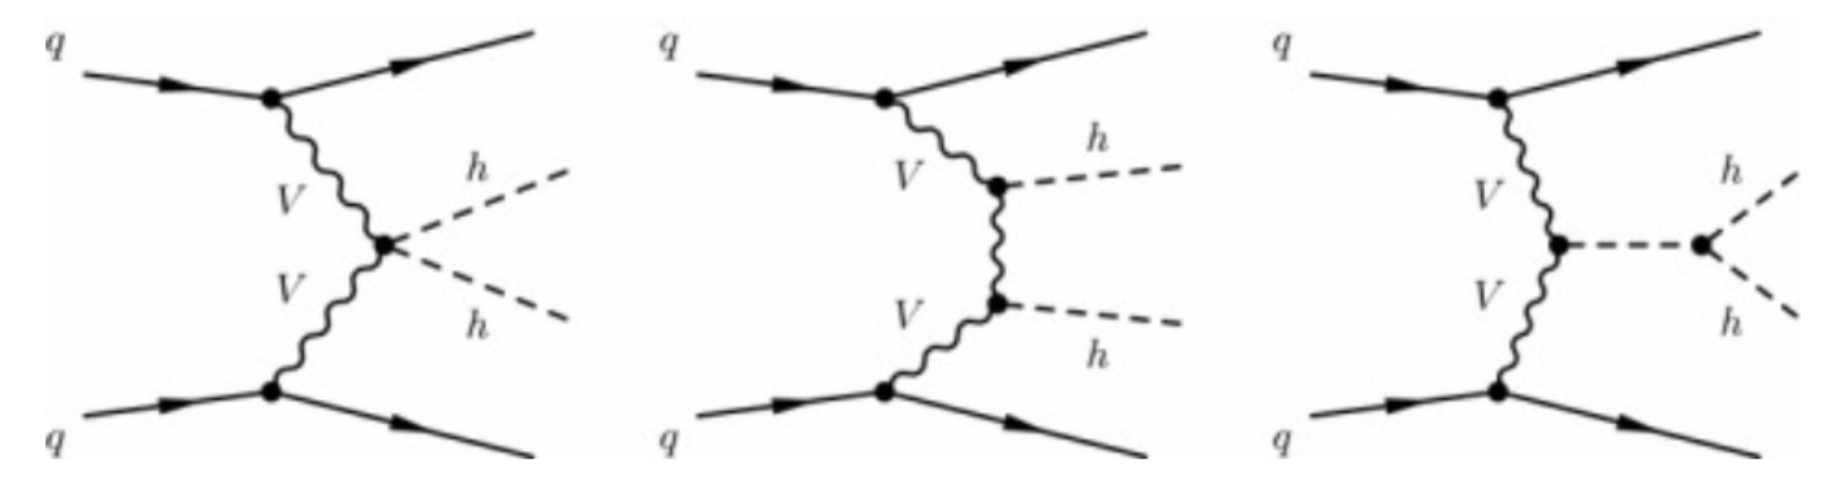
\includegraphics[width=0.85\textwidth]{fig/SMhh_VBF.png}
\caption{领头阶标准模型$hh$矢量玻色子融合产生过程。}
\label{fig:diagram_SMhh_VBF}
\end{figure}

图\ref{fig:diagram_SMhh_VBF}总结了不同$hh$产生过程截面随$\sqrt{s}$的变化情况。
\begin{figure}[h]
\centering
 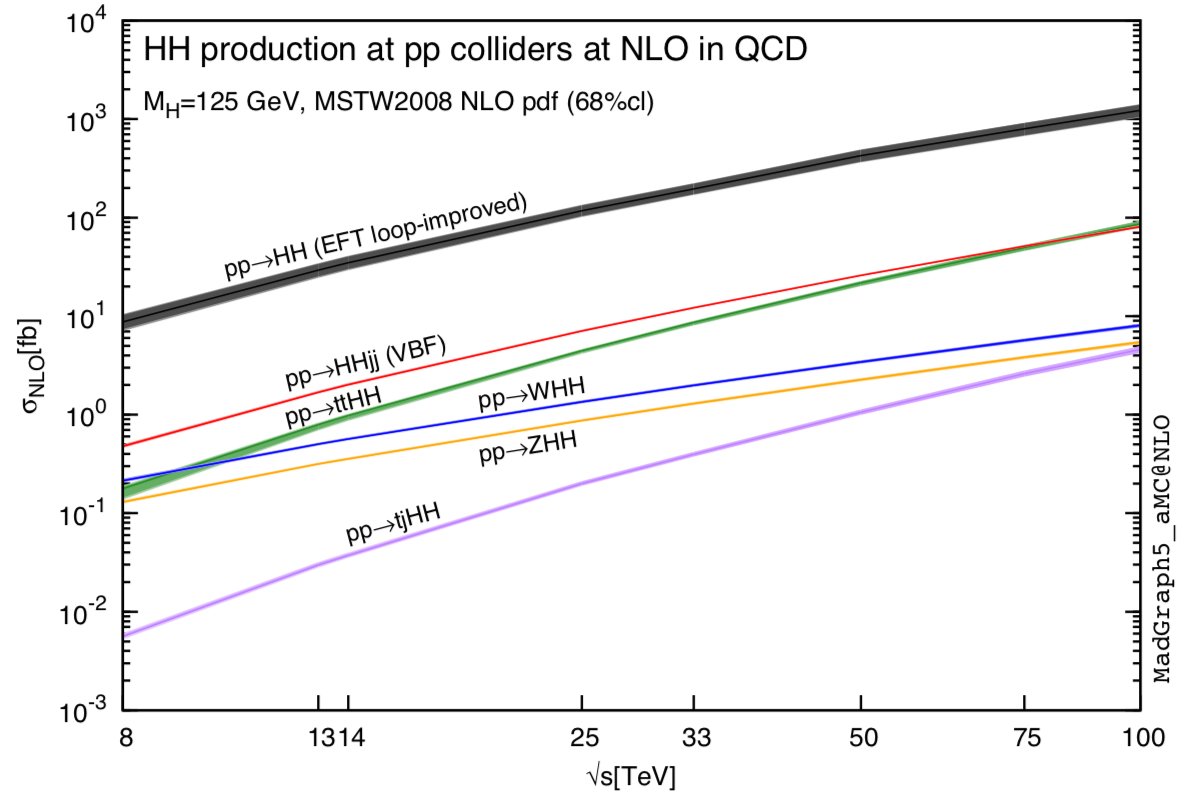
\includegraphics[width=0.85\textwidth]{fig/HH-xsec.png}
\caption{QCD次领头阶$hh$各产生模式的截面随$\sqrt{s}$变化情况\cite{Frederix:2014hta},包括胶子融合,矢量玻色子融合,顶夸克对,$W/Z$玻色子关联以及单顶夸克模式。
这里$H$指代标准模型Higgs,线宽代表不确定度,包括scale和PDF。}
\label{fig:diagram_SMhh_VBF}
\end{figure}
对于13 TeV质子质子对撞,考虑QCD次次领头阶和次次领头阶对数求和以及次领头阶有限顶夸克质量影响,几种$hh$产生过程的截面\cite{deFlorian:2016spz}总结在表\ref{tab:hh_predicted_xs}。\footnote{目前已有新的计算结果\cite{Grazzini:2018bsd,deFlorian:2013jea},但本文$hh$分析使用列出的计算值。}:
\begin{table}[h]
\centering
\scalebox{0.75}{
\begin{tabular}{ccc}
\hline
\hline
Production porcess   &Cross section [fb]    &Order of calculation \\
\hline
${gg\rightarrow hh}$  &$33.49+(\text{scale})^{+4.3\%}_{-6.0\%}\text{theory}^{+5\%}_{-5\%}(\alpha_s)^{+2.3\%}_{-2.3\%}\text{PDF}^{+2.1\%}_{-2.1\%}$  &NNLO+NNLL QCD\\
${\text{VBF}\rightarrow hh}$ &$1.62+(\text{scale})^{+2.3\%}_{-2.7\%}(\text{PDF})^{+2.3\%}_{-2.3\%}$ &NLO QCD\\
$gg\rightarrow hhh$ &$0.0632+(\text{scale})^{+16.1\%}_{-14.1\%}(\text{PDF})^{+3.4\%}_{-3.4\%}$ &NLO QCD \\
\hline
\hline
\end{tabular}}
\caption{13 TeV质心系能量下标准模型$hh$(假设$m_h$= 125.09 GeV, 但对于$gg\rightarrow hhh$,
$m_h$=125 GeV)产生截面理论预测值(fb)。}
\label{tab:hh_predicted_xs}
\end{table}
%其中第一项误差是scale,第二项代表顶夸克质量影响,第三项是QCD耦合常数,第四项是PDF影响。
%\begin{itemize}
% \item 胶子融合:$\sigma_{gg\rightarrow hh}=33.49+(\text{scale})^{4.3\%}_{-6.0\%}\text{theory}^{+5\%}_{-5\%}\text{\alpha_s}^{+2.3\%}_{-2.3\%}\text{PDF}^{+2.1\%}_{-2.1\%}$ fb;
% \item 矢量玻色子融合:$\sigma_{\text{VBF}\rightarrow hh}=1.62^{2.3\%}_{-2.7\%}\pm2.3\%$ fb;
% \item 胶子融合产生三Higgs:$\sigma_{gg\rightarrow hhh}=0.0632^{16.1\%}_{14.1\%}\pm3.4\%$ fb.
%\end{itemize}

\subsection{超出标准模型希格斯对产生}
虽然目前Higgs的测量结果越来越符合标准模型预期,但125 GeV的质量会有精细调节问题,如果有TeV量级的新粒子,不自然的问题就解决了。
在许多超出标准模型中,$hh$产生截面既可以通过非共振态也可以通过共振态模式增强。
对于非共振态模式中,可以通过修改$\lambda_{h\bar{t}t}$顶点\cite{Grober:2010yv,Contino:2012xk}或者一个新的带色荷标量粒子\cite{Kribs:2012kz};
还可以通过增强$\lambda_{hhh}$自耦合顶点,如图~\ref{fig:BSMhh_triangle}
中的绿圈所示。非共振态增强可以表述为超出标准模型产生截面与标准模型产生截面比值,对于希格斯自耦合顶点增强而言,等价于耦合常数增强,
即$\kappa_{\lambda}=\lambda/\lambda_{SM}$,从标准模型电弱测量得知,其被限制在$(-14, 17.4)$\cite{Kribs:2017znd}范围内。而且值得指出的是,
不同的$\kappa$对希格斯对产生有不同的影响\cite{Frederix:2014hta},图\ref{fig:HH_xs_kappa_14TeV}展示希格斯对产生截面随$\kappa$的变化情况。
在高$\lambda$区($|\kappa_{\lambda}|>10$),非共振态干涉贡献主要来自于自耦合顶点。
$\kappa$的确认可以通过测量希格斯对产生截面得到,这是$hh$研究的重要目标。
\begin{figure}[h]
\centering
 \begin{subfigure}[b]{0.33\textwidth}
  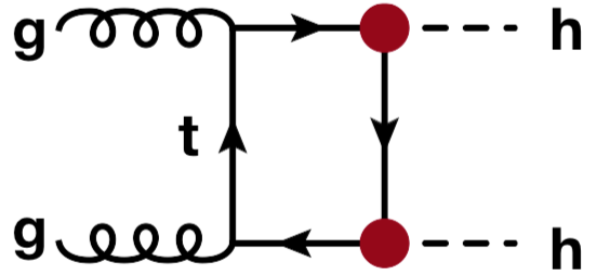
\includegraphics[width=0.85\textwidth]{fig/BSM_hh1.png}
  \caption{}
  \label{fig:BSMhh_box}
  \label{fig:diagram_BSMhh_box}
 \end{subfigure}
 \begin{subfigure}[b]{0.33\textwidth}
  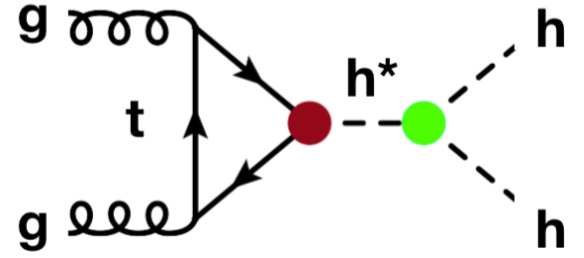
\includegraphics[width=0.85\textwidth]{fig/BSM_hh2.png}
  \caption{}
  \label{fig:BSMhh_triangle}
  \label{fig:diagram_BSMhh_triangle}
 \end{subfigure}
 \begin{subfigure}[b]{0.33\textwidth}
  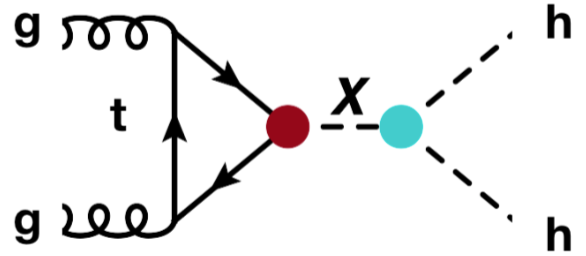
\includegraphics[width=0.85\textwidth]{fig/BSM_hh3.png}
  \caption{}
  \label{fig:BSMhh_resonance}
 \label{fig:diagram_resonant_hh}
 \end{subfigure}
\caption{超出标准模型希格斯粒子产生模式,其中\ref{fig:BSMhh_box}和\ref{fig:BSMhh_triangle}通过修改希格斯粒子耦合顶点常数实现,\ref{fig:BSMhh_resonance}则通过中间态高质量粒子$X$实现。}
\label{fig:diagram_BSM_hh}
\end{figure}

\begin{figure}[h]
\centering
 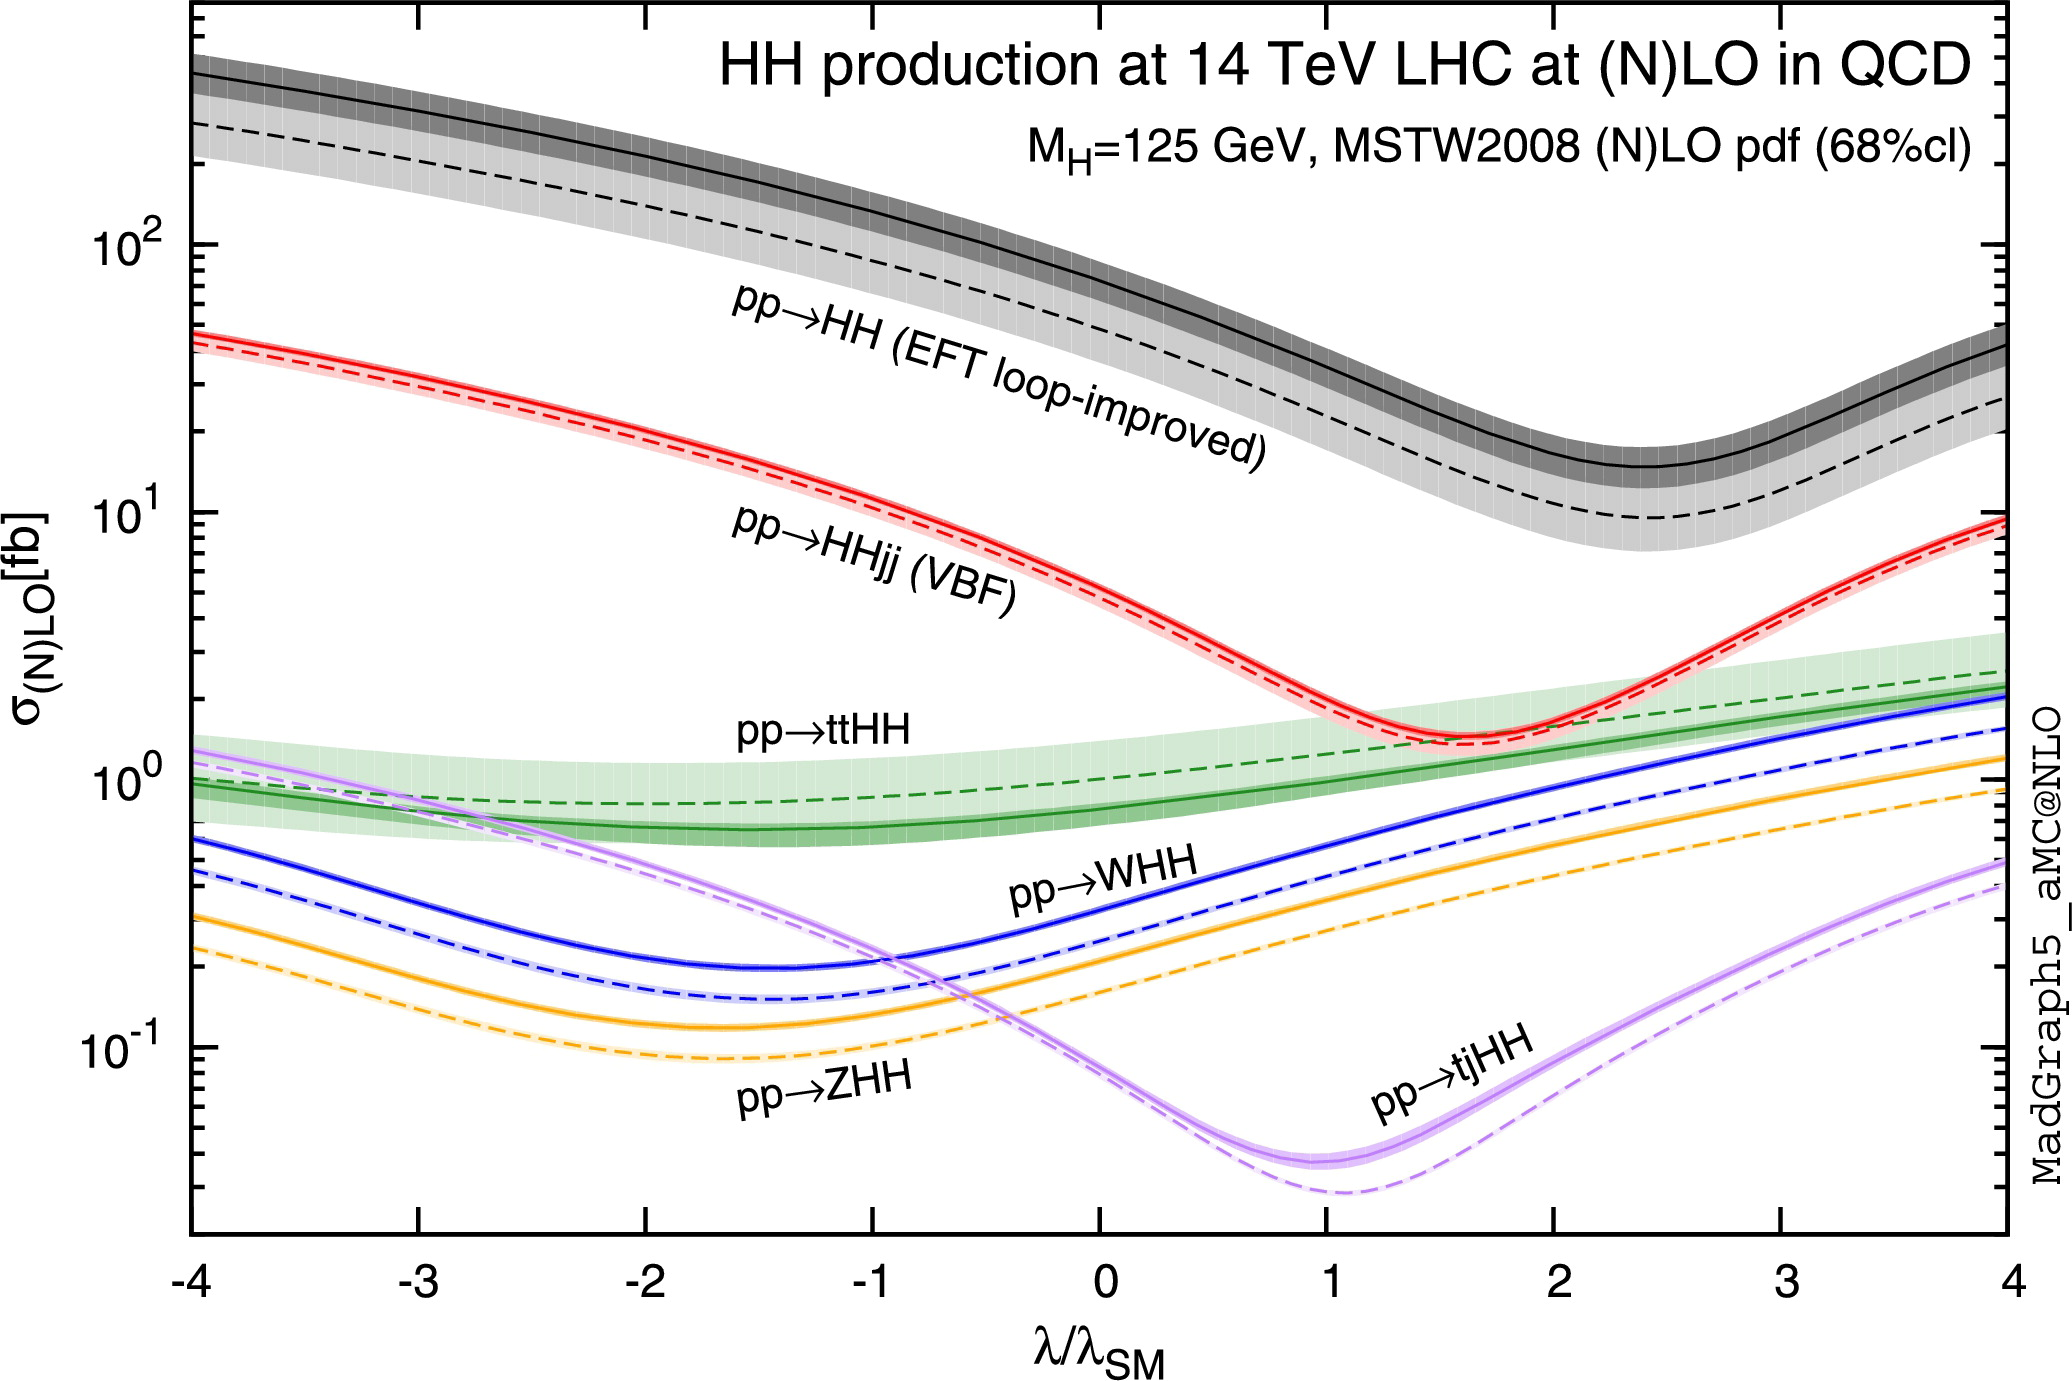
\includegraphics[width=0.85\textwidth]{fig/HH_xs_kappa_14TeV.jpg}
  \caption{14 TeV质心系能量下希格斯粒子对QCD(次)领头阶的产生截面随自耦合系数的变化情况,其中浅色虚线(深色实线)对应 领头阶 (次领头阶) 结果,其线宽代表来自scales和PDF的系统误差。 
  $\kappa$=1表示标准模型希格斯对产生。}
  \label{fig:HH_xs_kappa_14TeV}
\end{figure}

理论上比较容易引入一个新的与希格斯粒子耦合的标量粒子,从而使得希格斯对产生截面增大。一个简单的扩展是2HDM~\cite{2HDMTheory},它有两个希格斯二重态,
从而有5个希格斯玻色子,分别是$h$(轻标量Higgs,一般看作发现的标准模型Higgs),$X$(重标量Higgs),$A$(重赝标量Higgs),$H^{\pm}$(两个带电Higgs)。
为了避免树图阶味道改变中性流,2HDM应用分立对称性使得带电费米子只与一个希格斯二重态耦合。

\subsection{类希格斯对产生}
以上模型局限在$hh$中的$h$为标准模型希格斯粒子,它的质量为125 GeV,$h\rightarrow b\bar{b}$具有最大的衰变分支比。
但是我们也可以研究$h$不是标准模型粒子的情况,如在模型\cite{ExoticHiggsTheory}中,除了常规2HDM中的粒子,还额外引入一个实标量粒子$S$,
它被假设与希格斯粒子具有一样的耦合性质,唯一不同之处是质量,那么在$m_S>135$ GeV时(图\ref{fig:SM-HIGGS-BR}),$h\rightarrow WW$具有最大的分支比,
这是本文4$W$末态分析的动机之一。
\begin{figure}
\centering
 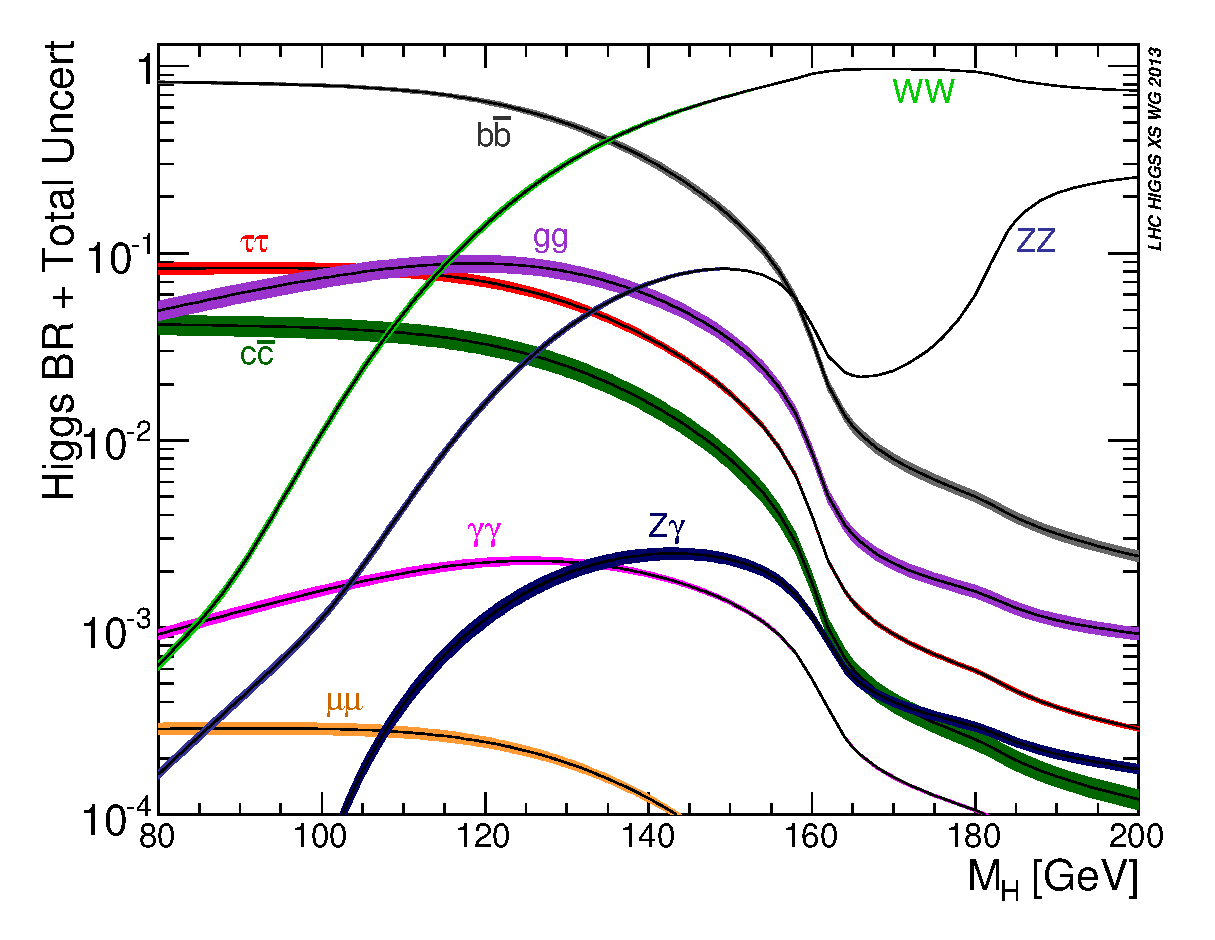
\includegraphics[width=0.75\textwidth]{fig/Higgs_BR_LM_RECT.eps}
 \caption{实标量希格斯粒子衰变分支比随质量分布,线宽表示不确定度。\cite{SM-HIGGS-BR}}
 \label{fig:SM-HIGGS-BR}
\end{figure}
%\subsection{希格斯对衰变}
%希格斯粒子的寿命只有$1.56\times10^{-22}~$s,在对撞顶点即衰变,表\ref{fig:HH_br}总结了$hh$的主要衰变道的分支比。在\RunOne ,ATLAS研究过$b\bar{b}b\bar{b}$\cite{Aad:2015uka},
%$b\bar{b}\gamma\gamma$~\cite{Aad:2014yja},$b\bar{b}\tau^{+}\tau^{-}$和$WW^{*}\gamma\gamma$,均没有观测到数据与预期的明显偏差。
%对于非共振态模式,其截面上限为0.69 pb,对应$\kappa<$70。
%共振态模式的联合拟合截面上限总结在图\ref{fig:HH_run1_combined}。
%\begin{figure}[h]
%\centering
% 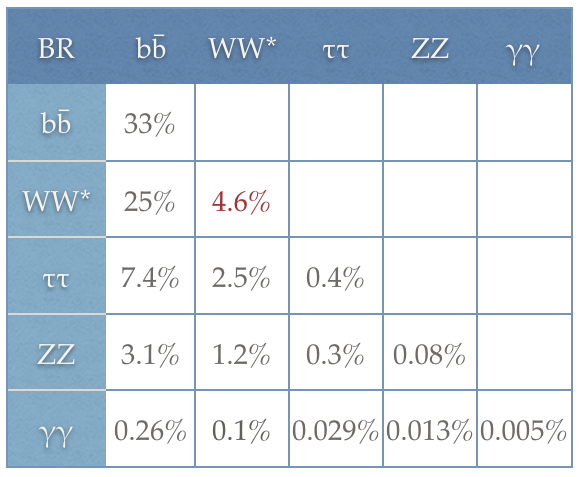
\includegraphics[width=0.75\textwidth]{fig/HH_br.png}
%  \caption{$hh$主要衰变道分支比,计算时假设$m_h$=125 GeV。}
%  \label{fig:HH_br}
%\end{figure}
%
%\begin{figure}[h]
%\centering
% 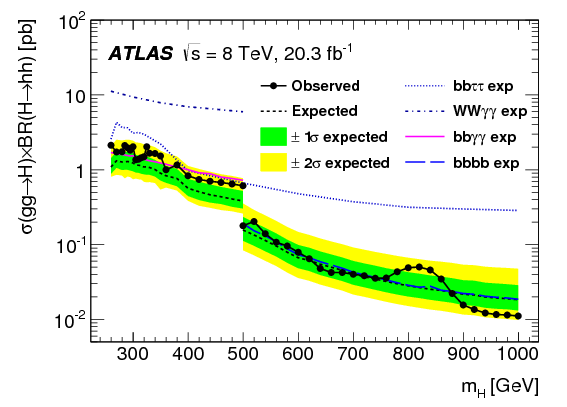
\includegraphics[width=0.85\textwidth]{fig/HH_run1_combined.png}
%\caption{在8 TeV质心系能量时$\sigma(gg\rightarrow H)\times\text{BR}(H\rightarrow hh)$的95\%置信度下的观测上限值与期望上限值,结果联合拟合了$b\bar{b}\tau\tau$, $WW^*\gamma\gamma$, $b\bar{b}\gamma\gamma$以及$b\bar{b}b\bar{b}$分析道。绿色和黄色区分别表示期望上限值的$\pm 1\sigma$和$\pm 2\sigma$,500 GeV以上的提升得益于$b\bar{b}b\bar{b}$的加入。}
%\label{fig:HH_run1_combined}
%\end{figure}
%
%现就一些衰变道作出简要概述:
%\begin{itemize}
% \item $b\bar{b}b\bar{b}$:它具有最大的衰变分支比,是$hh$搜寻的主要分析道,能够重建Higgs以及$X$的质量,但是其分辨率受限于$b$喷注重建及鉴别。在低$m_X$区,
% 因为$b$喷注触发效率太低,其显著性较低;但是在高$m_X$区,两个$b$喷注倾向合并,可以重建两个large-$R$~$b$喷注,而且得益于提高的$b$喷注触发效率,其显著性得到提高。
% \item $b\bar{b}W^{+}W^{-}$:具有第二大分支比,但是$t\bar{t}$本底限制了显著性,目前ATLAS正在积极研究优化策略。
% \item $b\bar{b}\gamma\gamma$:虽然截面不大,但是受益于较干净的双光子本底以及很好的光子分辨,在低$m_X$区有显著优势,
% 但在高质量区,双光子的合并对光子鉴别造成影响,使得显著性下降。
% \item $b\bar{b}\tau^{+}\tau^{-}$:该道与前两个道具有相当的显著性,尤其是在低$m_X$区,其主要挑战是赝$\tau$的本底处理。
% \item $WW^{*}\gamma\gamma$:该道与上述衰变道相比具有较差的显著性,但是得益于双光子以及轻子化衰变的$W$玻色子,本底较少,是$hh$搜寻的重要补充。
% \item $WW^{*}WW^{*}$:该道是本文$hh$分析的研究题目,将在章节\ref{}详细讲述。
% \item $WW^{*}\tau\tau, \tau\tau\gamma\gamma, \tau\tau\tau\tau, b\bar{b}ZZ, WWZZ$:这些衰变道的分支比都很小,均不能或者部分重建Higgs,还未公开发表过结果。
% 但是随着ATLAS累积更多的数据,使用单举策略\footnote{$WW^{*}\gamma\gamma$和$WW^{*}WW^{*}$也纳入其中},即以它们的衰变物进行分类,如轻子数,
% 不明显关注$hh$衰变中间态,而后进行优化,最后联合拟合得出结果,也许可以为$hh$搜寻作出重要贡献。
%\end{itemize}

\chapter{LHC和ATLAS实验}\label{chap:lhc_atlas}
\section{大型强子对撞机} \label{sec:LHC}
座落在瑞士法国边境的大型强子对撞机(LHC)是目前世界上最大,能量最高的对撞机,其对撞环(储存环)在地下100米,周长为27公里。
%它与之前的大型正负电子对撞机(LEP)使用同样的隧道,并沿用部分加速环。
%LHC可以前所未有的速率及能量提供质子-质子和铅-铅对撞,本文将讨论质子-质子对撞。LHC的质子-质子对撞的设计目标是提供质心系能量为14 TeV,平均瞬时亮度可达
%$10^{34} \text{cm}^{-2}s^{-1}$。关于LHC的详细论述可见~\cite{Evans_2008} \\
在LHC储存环上,有四个相互作用点(实验),分别是ATLAS~\cite{ATLAS_Collaboration_2008},CMS~\cite{CMS_Collaboration_2008},LHCb~\cite{LHCb_Collaboration_2008}以及ALICE~\cite{ALICE_Collaboration_2008},其相对位置如简图~\ref{fig:LHC_schematic}所示。
ALTAS和CMS是多用途探测器,主要为了检验标准模型和发现TeV量级新物理,随后会进一步介绍ATLAS探测器。
LHCb实验主要用于CP破坏以及$b$强子稀有衰变的精确测量。ALICE实验主要研究重离子对撞。
本文将讨论质子-质子对撞和ATLAS实验。
\begin{figure}[h]
\begin{center}
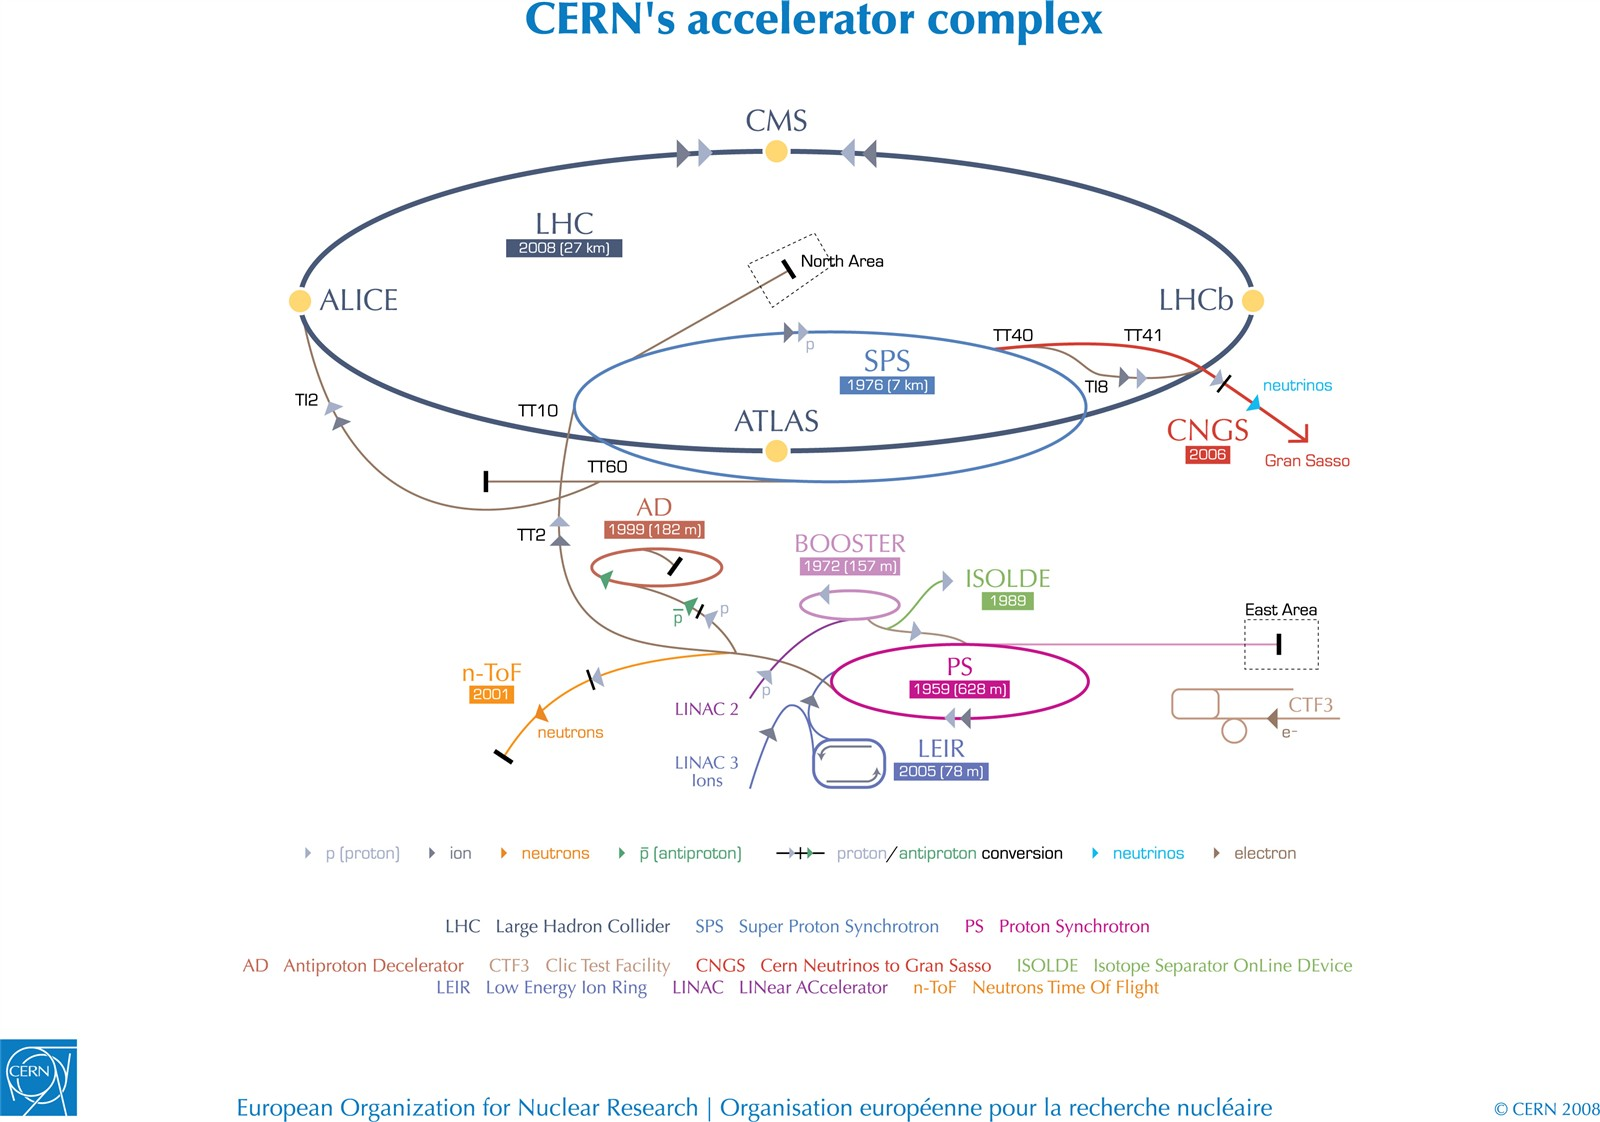
\includegraphics[width = 0.9\textwidth,angle=-90]{fig/LHC-shematic.jpg}
\caption{LHC概览} \label{fig:LHC_schematic}
\end{center}
\end{figure}

\subsection{质子加速过程}
LHC的设计目标是提供质心系能量为14 TeV,平均瞬时亮度可达$10^{34} \text{cm}^{-2}s^{-1}$的质子-质子对撞。
质子来源于电离氢气,而后会经历以下加速过程:
\begin{itemize}
  \item 通过线性加速器(Linac2)加速到50 MeV($\beta\approx5\%$);
  \item 注入到质子同步推进器(Proton Synchrotron Booster),加速至1.4 GeV($\beta\approx70\%$);
  \item 质子同步器(Proton Synchrotron)加速至25 GeV($\beta\approx99.9\%$);
  \item 超级质子同步器(Super Proton Synchrotron)提升至450 GeV($\beta\approx99.9998\%$);
  \item 注入储存环上的两条束流管,一条顺时针,另一条逆时针转圈,每次注入(fill)大约花费4分钟。
  \item 最终通过储存上的超导高频腔加速到6.5 TeV。
\end{itemize}
在每次注入后LHC可持续对撞几小时,直到束流密度下降到一定阈值,而后束流被导出,一个新的循环开始。

\subsection{亮度}
LHC的瞬时亮度公式如下:
\begin{equation}
\mathcal{L}=\frac{N_{b}^{2}f_{r}n_{b}F}{4\pi\varepsilon_{n}\beta^{*}}
\end{equation}
其中$N_b$(束流团所含质子数),$n_b$(储存环中运行束流团数),$f_{r}$(束流团旋转频率)以及$\varepsilon_n$(束团归一横向发射度,描述粒子横向扩散)由质子加速过程决定;
而$\beta^{*}$是在对撞点的所谓振幅函数,它的性质由聚焦磁铁决定;F是为修正束团对撞角度偏差的束流形状因子,一般小于1。$\varepsilon_{n}\beta^{*}$正比于束流横向面积,
那么越小的横向发射度或者越小的振幅函数意味着更窄的束流,对撞频率就越高。关于LHC亮度的重要参数如表~\ref{tab:lhc_run_summary}所示,需要注意的是,自LHC开机以来,一直在进行优化,一些所列
参数已经超过设计指标,比如最大瞬时亮度,其已在2016年运行时超过$10^{34}~\text{cm}^{-2}~\text{s}^{-1}$,主要是因为更小的$\beta^{*}$和优化的形状因子。相应地,pileup数也随之增加,见图\ref{fig:mu_2015_2016}。
2015年到2017年LHC亮度及ATLAS数据收集情况总结在图\ref{fig:data_taking}。
\begin{table}[h]
\centering
\scalebox{0.75}{
\begin{tabular}{ccccccc}
\hline
Beam/collision parameters    &2015       &2016  &Nominal design (if available)\\
Center-of-mass energy ($\sqrt{s}$) [TeV]     &13   &13    &14 \\
Bunch spacing [ns]   &50-25   &25    &25 \\
Bunch revolution frequency ($f_{r}$) [kHz]  &11.245  &11.245  &11.245 \\
Max. number of bunches/beam ($n_{b}$)   &2232    &2208    &2808  \\
Max. charge per bunch colliding ($10^{11}~$p/bunch) &1.21   &1.31   &1.15 \\
Peak instantaneous luminosity [$10^{34}~\text{cm}^{-2}~\text{s}^{-1}$]  &0.5  &1.38  &1  \\
Max. pileup  &28.2   &52.2   & \\
Longest stable beams fill duration [h]  &24.3 &37.03  & \\
\hline
\end{tabular}}
\caption{LHC设计指标,以及在2015年和2016年的运行参数~\cite{LHC-Run-Summary}}
\label{tab:lhc_run_summary}
\end{table}

\begin{figure}[h]
\centering
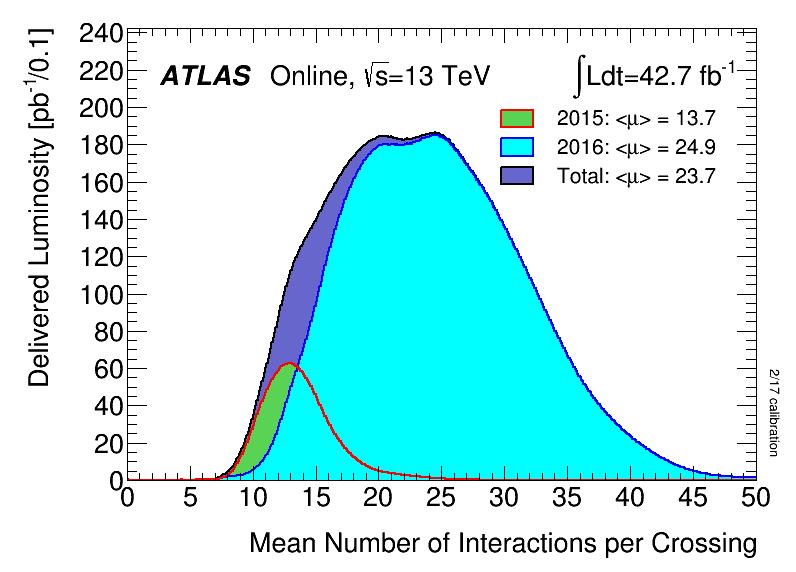
\includegraphics[width = 0.75\textwidth]{fig/mu_2015_2016.png}
\caption{ATLAS 2015年和2016年亮度-pileup分布。}
\label{fig:mu_2015_2016}
\end{figure}
\begin{figure}[!htbp]
    \centering
    \begin{subfigure}[b]{0.45\textwidth}
      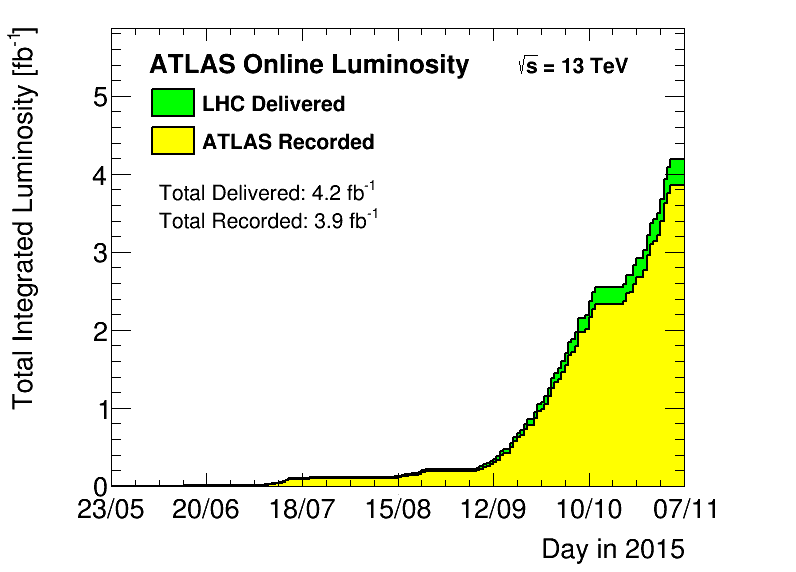
\includegraphics[width=\textwidth]{fig/sumLumiByDay.png}
      \caption{}
      \label{fig:data_taking_2015}
    \end{subfigure}%
    ~%add desired spacing
    \begin{subfigure}[b]{0.45\textwidth}
      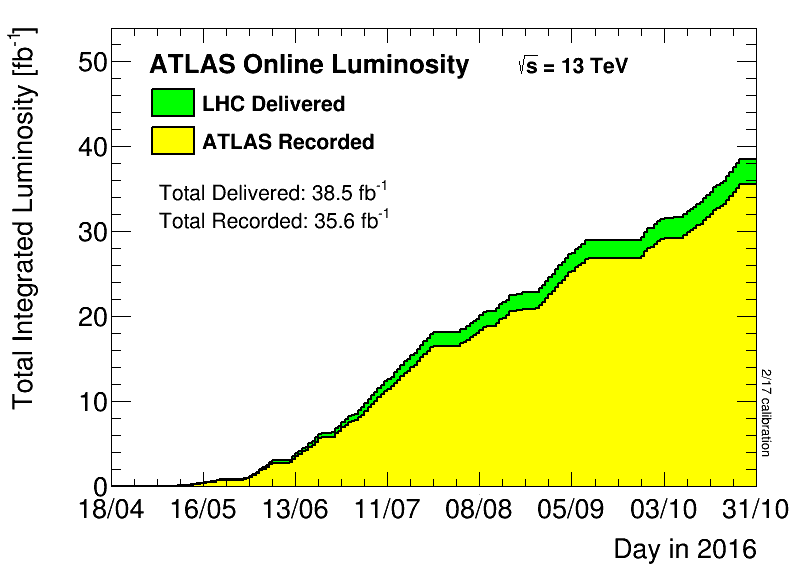
\includegraphics[width=\textwidth]{fig/sumLumiByDay_2016.png}
      \caption{}
      \label{fig:data_taking_2016}
    \end{subfigure} \\
    \begin{subfigure}[b]{0.45\textwidth}
      \centering
      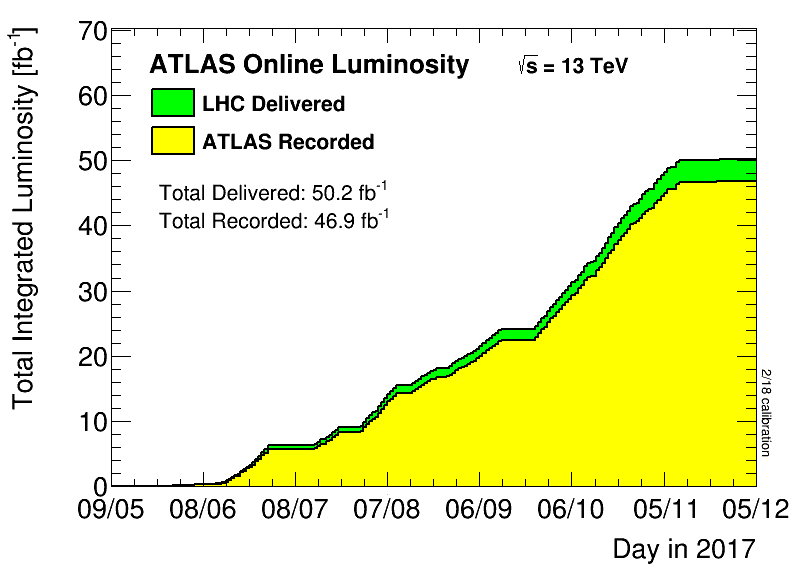
\includegraphics[width=\textwidth]{fig/sumLumiByDay_2017.png}
      \caption{}
      \label{fig:data_taking_2017}
    \end{subfigure}
    \caption{ATLAS数据收集情况: (a)2015年, (b)2016年, (c)2017年。}
    \label{fig:data_taking}
\end{figure}

\section{ATLAS探测器} \label{sec:ATLAS}
ATLAS探测器座落在LHC储存环,它有25米高,44米长,总重大约7000吨。ATLAS探测器内层是内部径迹探测器(ID),其被直径为2.3米的超导螺线管包围,该超导线圈提供平行于
束流方向,大小为2 T的磁场;紧挨着ID是量能器系统,包括电磁量能器(EM)和强子量能器(HCal);最外层是$\mu$子探测器(MS)。本章将论述图~\ref{fig:ATLAS_schematic}所示的各个部分。

\begin{figure}[h]
\begin{center}
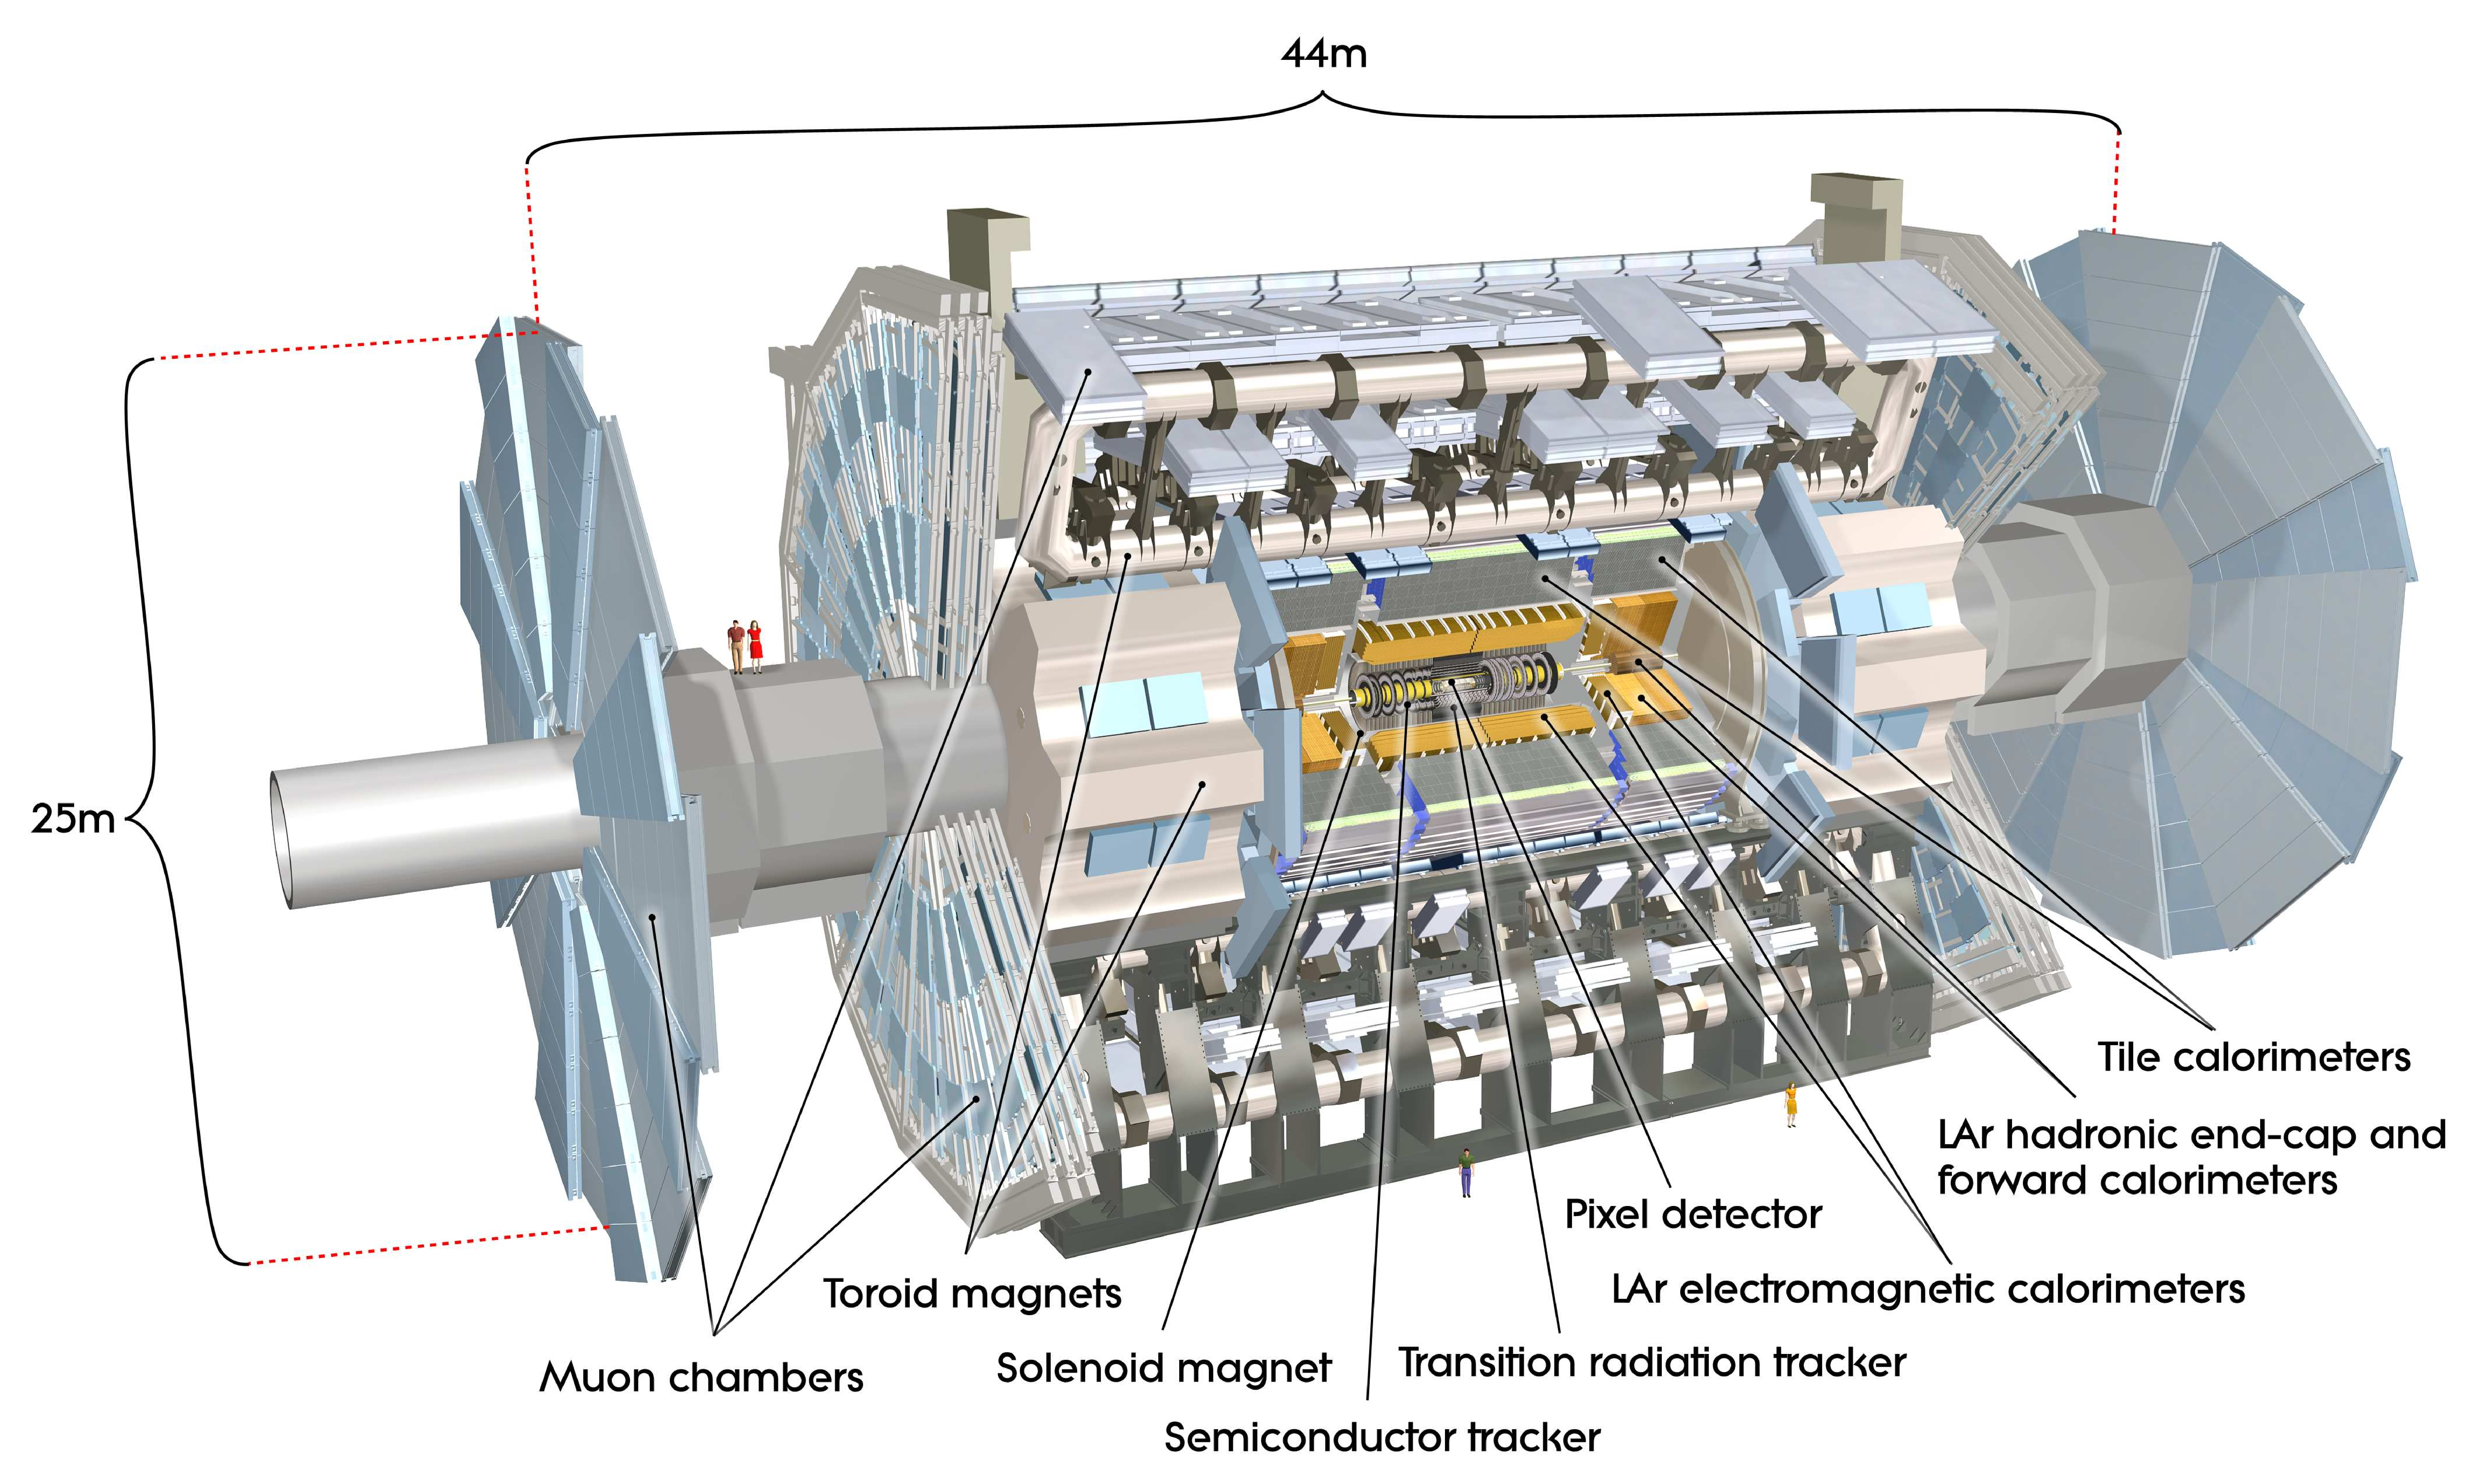
\includegraphics[width=0.9\textwidth]{fig/ATLAS_SE_Corrected7.pdf}
\caption{ATLAS探测器简图} \label{fig:ATLAS_schematic}
\end{center}
\end{figure}

\subsection{坐标系统}
ATLAS使用右手坐标系,其定义对撞点(IP)为原点,z轴为束流方向,正x轴指向环中心,正y轴则向上。在极角坐标系中,定义方位角$\phi$在(x, y)平面,大小从$-\pi$到$\pi$,极角$\theta$
从0到$\pi$,$\theta=0$时与正z轴同向。\\
赝快度定义为$\eta = -ln\tan(\theta/2)$,更大的$|\eta|$意味着粒子更靠近束流方向,在ATLAS一般称为更前向。
定义两个粒子的角距离$\Delta R=\sqrt{(\Delta\eta)^2+(\Delta\phi)^2}$。

\subsection{内部径迹探测器}
ATLAS内部径迹探测器主要用来精确寻迹(\pt > 0.1 GeV),可覆盖$|\eta|<2.5$。它包括三个子探测器,离束流中心距离从3.3 cm到101.6 cm,图~\ref{fig:ATLAS_ID_sideview}展示ID的
各个部分的分布。ID沉浸在通过铌钛超导螺线管产生的2 T轴向磁场中,线圈通过液氦冷却,温度为4.5 K。ID的强磁场可偏转带电粒子,通过测量径迹曲率可推出粒子动量。
\begin{figure}[h]
\begin{center}
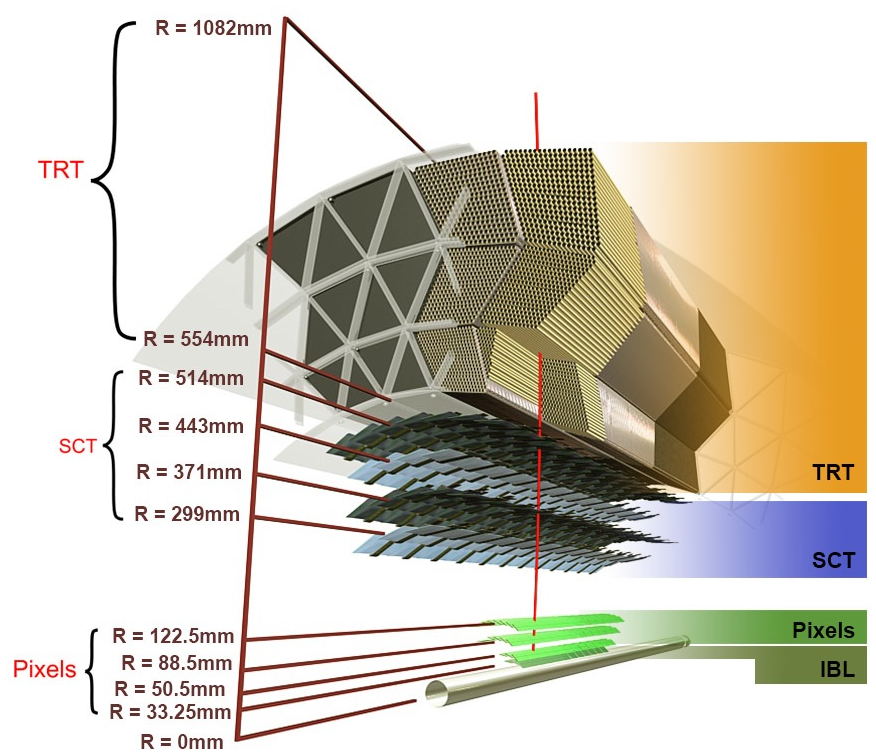
\includegraphics[width=0.9\textwidth]{fig/ATLAS_ID_sideview.png}
\caption{ATLAS内部径迹探测器} \label{fig:ATLAS_ID_sideview}
\end{center}
\end{figure}

%\subsection{像素探测器和IBL}
像素探测器(Pixel detector)围绕着束流中心,是离束流最近的系统,会经受最高密度的粒子束流,因此在ATLAS所有子探测器中具有最高的分辨率。Pixel在桶部区有四层,由1744个模块组成(module),端盖区有三层,含有288个模块。桶部区的最内层(IBL)在Run 1和Run 2之间安装,主要用于提高\bjet 鉴别。每个Pixel模块含有46080个电子学读出道,Pixel探测器总共有8千万读出道。
每个模块大小为$50\times400 \mu ~\text{m}^{2}$(IBL模块为$50\times250 \mu ~\text{m}^{2}$),其位置分辨率可达10 $\mu m$(r-$\phi$)和115 $\mu m$(z方向)。

硅微条探测器(SCT)桶部区有四层,端盖区有9层。每个SCT模块只能提供一维位置信息,所以每层SCT两个模块背靠背以一定角度粘贴在一起,加上模块本身所在位置即可
提供三维位置信息。一般SCT的分辨率为17 $\mu m$(r-$\phi$),580 $\mu m$(z方向)。SCT的总读出电子学道为630万。

穿越辐射探测器(Transition Radiation Tracker,称TRT)由大约30万,直径为4 mm充满70\%氙气,20\% CF$_4$,10\%二氧化碳的漂移管组成,桶部区的漂移管与轴线平行,端部区的漂移管
则成辐射状,其总的电子学读出道达35万。带电粒子穿过漂移管电离气体,电离电子在电压作用下达到管中心丝。桶部区(端部)只提供$r-\phi$(r-z)方向的位置测量,每条管的位置分辨率为130 $\mu\text{m}$。
TRT管层含有聚丙烯纤维和箔层,带电粒子穿过它们的边界时发射X射线,
其强度与入射粒子能量成正比,X射线通过光电效应能够产生比电离电子幅度更大的信号。
%通过这种X射线在吸管气体中的光电效应产生的电子产生的信号具有比源自经过的颗粒的信号更高的振幅。 
入射电子动量接近1 GeV时即产生明显的穿越辐射,而$\pi$介子在$\mathcal{O(100)}$~GeV动量时才产生辐射,
这可有助于粒子鉴别。

ID可为粒子径迹重建提供36个着火点($\abseta < 2.0$)。联合这三个子探测器的信息,ID可测量\pt 低至400 MeV的带电粒子,
其相应的动量分辨率可由如下公式~\cite{ATLAS_Collaboration_2008}描述:
\begin{equation}
 \frac{\sigma_{\pt}}{\pt}=0.05\%\pt\oplus1\%
\end{equation}

\subsection{量能器}
ATLAS量能系统~\cite{ATLAS_Collaboration_2008}包括几个具有不同技术和粒度的组件,涵盖非常大的范围(\abseta <4.9)。 所有组件都是采样式取数,带有吸收材料,入射粒子经过产生电磁或强子簇射,这些簇射能量仅有一部分被灵敏层检测。 量能器会利用测试束流以及探测器模拟~\cite{4436305,Davidek_2009}进行刻度,并在碰撞数据中刻度。 
ATLAS量能器的布局如图~\ref{fig:Calorimeter_d3}所示。
\begin{figure}[h]
\begin{center}
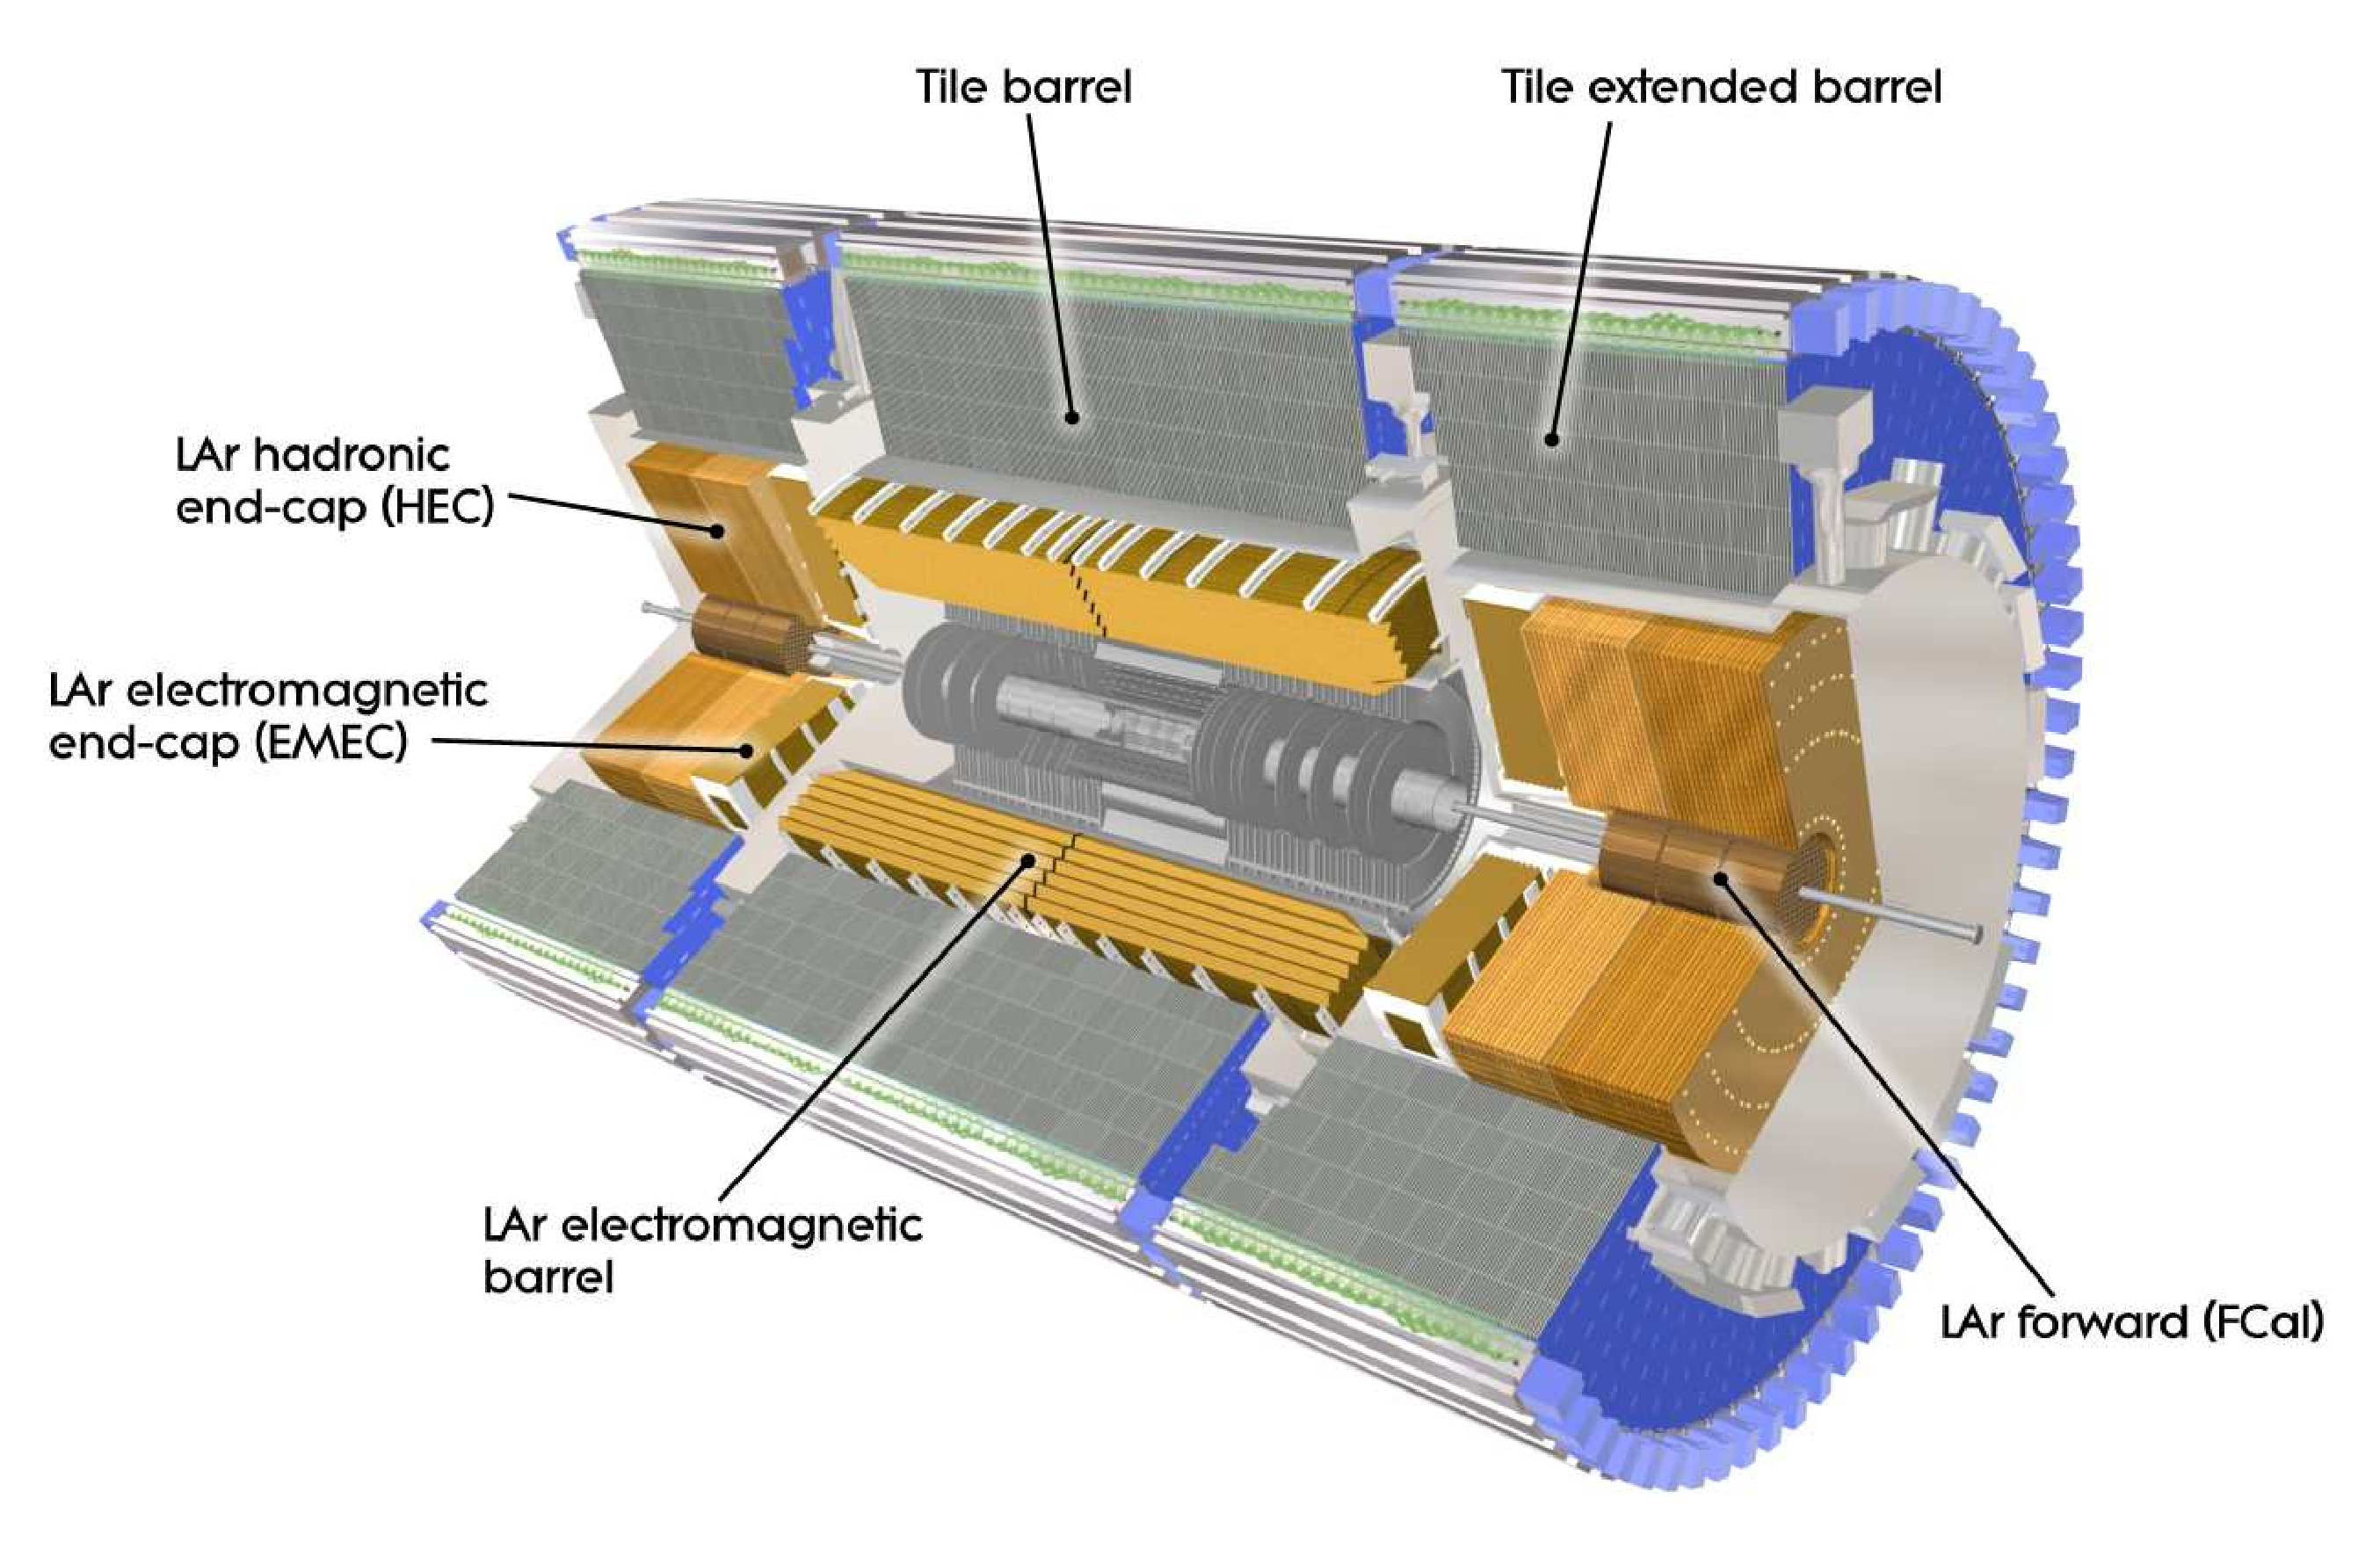
\includegraphics[width=0.9\textwidth]{fig/Calorimeter_d3.pdf}
\caption{ATLAS量能器布局} \label{fig:Calorimeter_d3}
\end{center}
\end{figure}

螺线管外部最里面的部分是电磁量能器,专门用于电子和光子的能量测量。它使用液氩(LAr)作为活性介质,具有优异的抗辐射性和能量分辨率,并容易产生电磁簇射。
读出单元是分成条状的电镀铜板电极。
EM桶部可覆盖到\abseta = 1.4,端盖系统延伸到\abseta = 3.2。
它分为3-4层,具有类似手风琴的几何形状,可提供完整的$\phi$覆盖,没有死区,并且在ID探测范围内(\abseta <2.5)具有精细的$\Delta \eta\times\Delta\phi$分辨,最小值为0.025$\times$0.025,可以分辨$\pi0\rightarrow \gamma\gamma$。
为了确保能够接收绝大数的电磁簇射,EM桶部厚度大于22个辐射长度(X0),端盖则大于24倍X0。
大多数服务设施都位于过渡区域,即$1.37<\abseta<1.52$。
%,能量测量部分缺乏,会有较差的能量测量表现。
EM能量分辨率可描述为~\cite{ATLAS_Collaboration_2008}:
\begin{equation}
\frac{\sigma_{E}}{E}=\frac{10\%}{\sqrt{E}}\oplus0.7\%
\end{equation}

强子量能器包围着电磁量能器,专门用于测量$\pi$介子和中子等强子的能量。 桶区$\abseta<1.7$由三层钢-塑料闪烁体采样量能仪(TileCal)组成,其在$\eta = 0$时总厚度为9.7倍相互作用长度($\lambda$),
以最大限度地减少强子簇射穿透HCal并到达外部$\mu$子光谱仪(punch-through)。
强子端盖量能器(HEC)覆盖$1.5<\abseta<3.2$,虽然使用铜作为被动材料并为平面状,但是与HCal采用相同的液态氩技术。
强子量能器的粒度比EM更粗,为$\Delta \eta\times\Delta\phi$为$0.1\times0.1$,
并且由于强子与材料核相互作用的性质,能量分辨率更差~\cite{ATLAS_Collaboration_2008}:
\begin{equation}
\frac{\sigma_{E}}{E}=\frac{50\%}{\sqrt{E}}\oplus3\%
\end{equation}

最后,3层前向量能计(FCal)覆盖$3.1<\abseta<4.9$以测量丢失横向能量和前向喷注。它也采用LAr技术,利用铜和钨分别作为第一层和最后两层的吸收材料。

\subsection{$\mu$子谱仪}
$\mu$子谱仪(MS)环绕着量能器,是ATLAS最外层的子探测系统,用于测量穿过ID和量能器的$\mu$子动量和位置。 MS系统有大约100万个电子学读出道,从半径5米延伸到10米,在\abseta =0处因为服务电缆有一个小间隙。
MS桶区由3个同心圆柱体组成,设计用于测量动量高于5 GeV的$\mu$子,其分辨率在100 GeV时为3\%。 端盖区有四个轮状部分,覆盖到$\abseta<2.7$。与ID类似,MS也可测量$\mu$子动量,
其磁场由大型空心环形磁体系统提供,大小在0.5~T和1~T之间。

$\mu$子室有两组系统:一组用于$\mu$子轨道的精确测量,第二组用于$\mu$子触发。精密腔室包括监测漂移管(MDT)\cite{Bauer:2016gyg}和阴极条带室(CSC)\cite{Argyropoulos:2009zz}。MDT涵盖$\abseta<2.7$的大部分区域,
 除了端盖最内层安装CSC区域$2.0<\abseta<2.7$。
 MDT由3cm直径的漂移管组成,其含有93\%氩和7\%CO$_{2}$的混合物。每根管具有单根钨-铼线,其在3kV的电压下操作,基于入射粒子产生的电离电荷的漂移时间可测量其相对位置。单管的典型空间分辨率低于100 $\mu\text{m}$,联合多层管可提升至约50~$\mu\text{m}$。

CSC由具有正交平面阴极的多丝比例室组成。它们可以处理更高的粒子流并且具有比MDT更高的辐射耐受性,因此被放置在粒子通量较大的前向区域$2<\abseta<2.7$。径向导线保持在1.9 kV的电势,并与每个条状阴极保持2.5 mm的距离。
在弯曲平面的CSC探测器寻迹分辨率约为60~$\mu\text{m}$并且具有高抗辐照性,因此用在MS的第一层。

不同的设计导致不同的电荷收集时间,MDT约为700 ns,CSC约为40 ns。
%收集时间的巨大差异是因为MDT和CSC的设计不同。
MDT为管状,在中心丝上施加电压,电场以$1/r^{2}$下降($r$是与中心丝的距离)。
而CSC是具有恒定电压差和恒定场的平坦腔室。
两个专用触发室提供快速测量,用于触发决策。$\mu$子事件的触发系统基于电阻板腔(RPC)\cite{Aielli:2006hg}仪器在桶区域$\abseta<1.05$,而薄间隙腔(TGC)\cite{Majewski:1984ag}用于端盖区域。 
RPC由平行电极板组成,它们相距2 mm并填充有$\text{C}_{2}\text{H}_{2}\text{F}_{4}$的气体混合物,工作电压为9.8 kV,
有非常好的时间分辨率,约为2 ns。TGC由多丝正比室组成,含有$\text{CO}_{2}$和$\text{n-C5H}_{12}$的气体混合物。
TGC的阳极线距离带状阴极1.4 mm,之间的电位差为2.9kV,时间分辨率为4 ns。
%环形磁铁在方位角平面上产生0.5T至1T的磁场。桶部中有八个矩形线圈,覆盖$\abseta <1.6$,每个端盖中有8个线圈,覆盖$1.4<\abseta<2.7$。线圈由铝,铜,铌和钛的混合物构成,并用液氦冷却至4.5K。MS的$\mu$子\pt~分辨率受到磁场不均匀性的限制。
\begin{figure}[h]
\begin{center}
 \begin{subfigure}[b]{0.45\textwidth}
      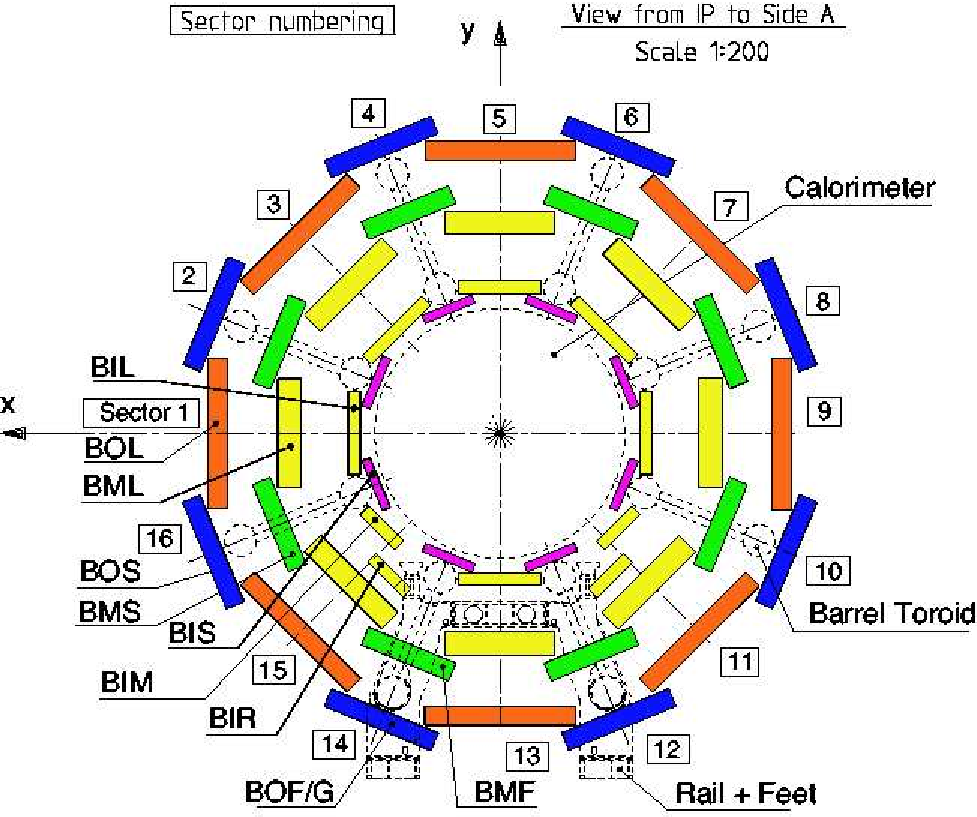
\includegraphics[width=\textwidth]{fig/Muon_sector_numbering.pdf}
      \caption{}
      \label{fig:muon_xy}
  \end{subfigure}
 \begin{subfigure}[b]{0.45\textwidth}
      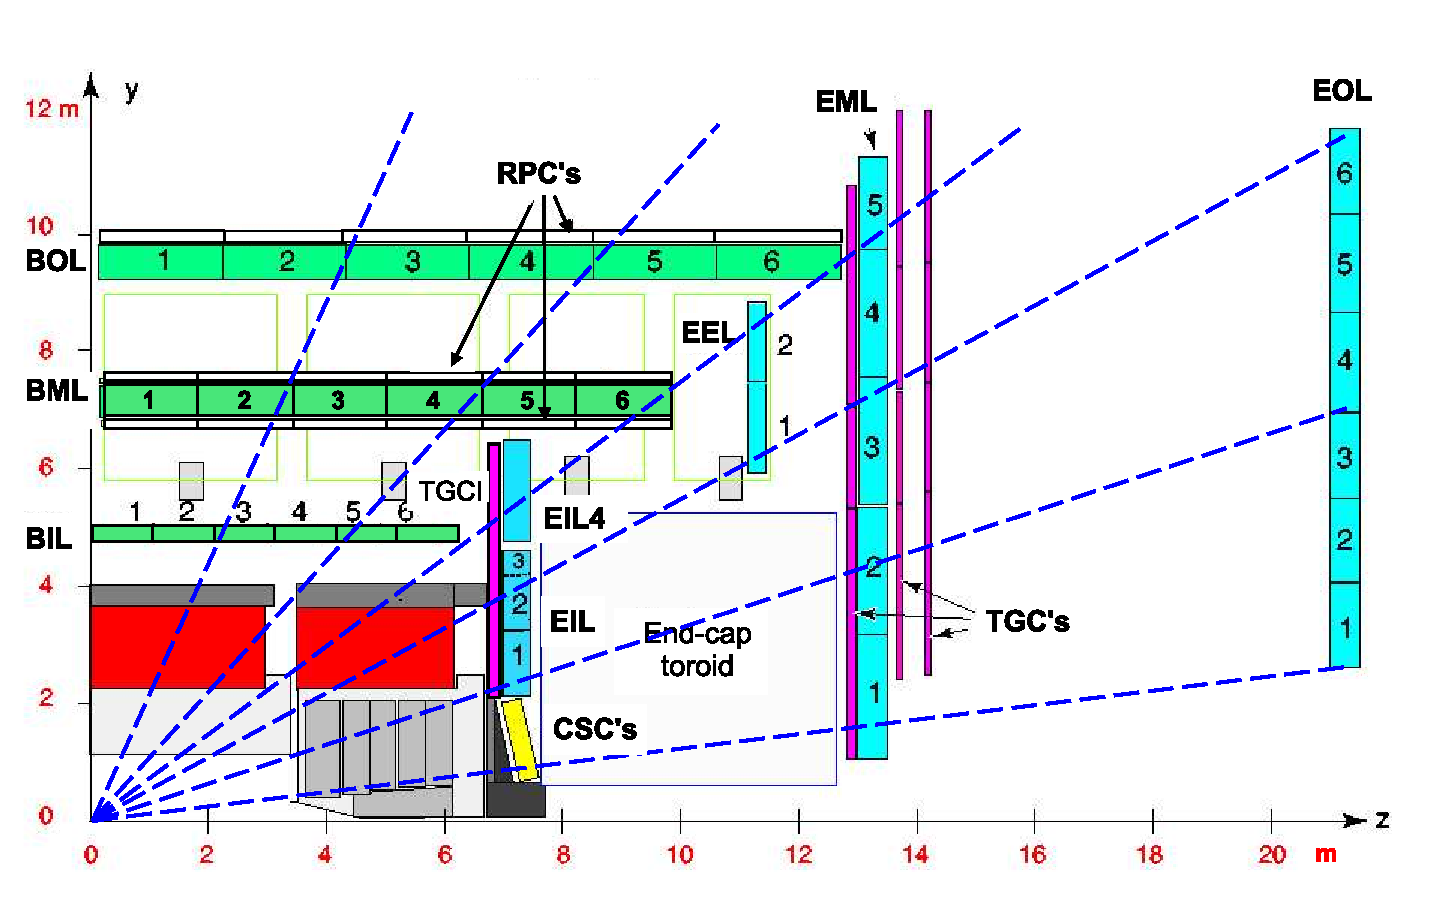
\includegraphics[width=\textwidth]{fig/Muon_rz_large_sect_6.pdf}
      \caption{}
      \label{fig:muon_rz}
  \end{subfigure}
\caption{(a) 与束流垂直方向($x-y$平面)的$\mu$子谱仪布局,它有三层同心圆柱,每层包含8个大室和8个小室,最外层半径大约为20米。(b) $y-z$平面的$\mu$子谱仪布局}
%,Cross-section of the muon system in a plane containing the beam axis (bending plane). Infinite-momentum muons would propagate along straight trajectories which are illustrated by the dashed lines and typically traverse three muon stations.} 
\label{fig:muon_overview}
\end{center}
\end{figure}

\subsection{触发和数据采集系统}
%由于数据存储容量和速率的限制,LHC每秒产生大量的事例必须经过实时筛选和在线触发\cite{Artz_2015},最终只有一小部分被记录。
%当前的ATLAS触发系统包括基于硬件使用来自量能器和$\mu$子系统粗略测量的触发(L1),以及基于软件的高级触发(HLT)。L1将事件发生率(这指bunch-crossing)从40 MHz降低到100 kHz,HLT进一步将其降低到1 kHz的平均记录速率\cite{Artz_2015}。ATLAS数据采集(TDAQ)系统的示意图如图\ref{fig:ATLAS_TDAQ}所示。
%L1触发系统执行初始事件选择并接受100 kHz速率的事件。它经过优化,可以快速做出决策。它联合量能器和MS的信息搜索高能量轻子,光子和喷注。电子和光子触发基于EM量能器中的能量沉积,这
%受限于EM本身分段。
%在强子量能器中,使用滑动窗口算法得到的触发元素形成的簇射最终构建候选喷注。
%一个触发元素是$0.2\times0.2(\eta-\phi)$单元格的总能量沉积,滑动窗口算法会在$4\times4$区域在特定阈值之上检查总$E_{T}$。$\mu$子触发基于触发室若干层着火点重合。
LHC束团间距为25 ns,那么束团碰撞率为40 MHz,质子非弹性散射率接近1 GHz,平均pileup数为23.7,考虑到电子读出系统和数据存储能力的限制,ATLAS仅能处理并存储极少数的事例。
ATLAS触发和数据采集系统(TDAQ)\cite{Aaboud2017}是探测器的基本组成部分,它负责决定是否为以后的离线研究保存事件。

TDAQ有两级:基于硬件的使事例率降低至100 kHz的Level-1触发器(L1),以及基于软件的高级触发器(HLT)系统。HLT使用4万个CPU,并在一次LHC注入期间以1 kHz的平均速率选择事件,这是离线计算模型和存储可以处理的最大值。

L1触发器包括中央触发处理器(CTP),它处理来自L1量能器(L1Calo)和L1~$\mu$子(L1Muon)触发子系统的输入。L1Calo直接从量能器获取信息。L1Muon利用桶部($\abseta<1.0$)RPC和$1.0<\abseta<2.4$区的TGC进行测量。
为了应对更高的事件发生率并有效地选择感兴趣的物理事件,在2016年一个称为L1拓扑处理器(L1Topo)\cite{Simioni:2014nha}的新元素添加到L1中。L1Topo系统从L1Calo和L1Muon获取信息,可以计算不变质量等物理变量以用于L1决策。
由于L1电子设备的延迟为2.5 $\mu\text{s}$,CTP也应用预防性死时间,设置L1连续两次接受决策之间的最短时间以避免重叠读出窗口,并限制在给定束团对撞数目内L1接受决策数以避免前端缓冲区溢出。

在L1触发接受之后,HLT使用更细粒度的量能器信息,来自MS的精确测量以及来自ID的径迹信息来处理事件。为了最大限度地提高效率,HLT软件经过调整,使算法和选择尽可能接近离线重建。
HLT接受的事件最终存储在磁盘上,并导出到CERN计算中心进行离线重建。根据需要,HLT可以处理来自L1处识别的感兴趣区域(RoI)或来自完整探测器的信息。ATLAS触发系统的完整方案如图~\ref{fig:ATLAS_TDAQ}所示。
\begin{figure}[h]
\begin{center}
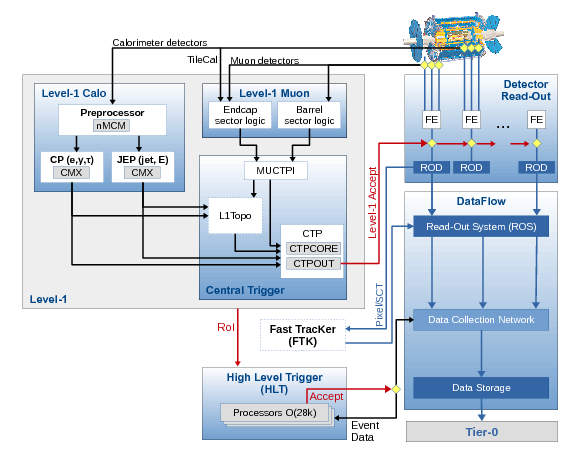
\includegraphics[width=0.75\textwidth]{fig/content_tdaq_figures_tdaq-run2-schematic.png}
\caption{ATLAS TDAQ系统\cite{Aaboud2017},图中着重标注触发相关部分。L1Topo与FTK正在研究,并未包括本文的结果中。} \label{fig:ATLAS_TDAQ}
\end{center}
\end{figure}

L1和HLT的触发决策根本上是由物理分析决定的,不同物理分析处理不同的物理对象,
而所有这些物理对象归纳起来则给出所谓的触发菜单。菜单中的主要触发器涵盖了各种ATLAS物理搜索所需的所有信号,包括电子、$\mu$子、光子、$\tau$轻子、喷注和丢失能量(MET)。
触发菜单组成和触发阈值针对若干亮度范围进行了优化,以便最大化实验的物理输出并且满足ATLAS探测器读出速率和带宽限制。
许多ATLAS分析的主要特征信号,包括$hh\rightarrow 4W$搜索,是电子或者$\mu$子。 因此,在事件中需要存在至少一个$\pt>$25 GeV轻子的触发占据可用带宽的很大一部分,如图\ref{fig:Trigger_singlelepton}所示。
\begin{figure}[h]
\begin{center}
\begin{subfigure}[b]{\textwidth}
\centering
   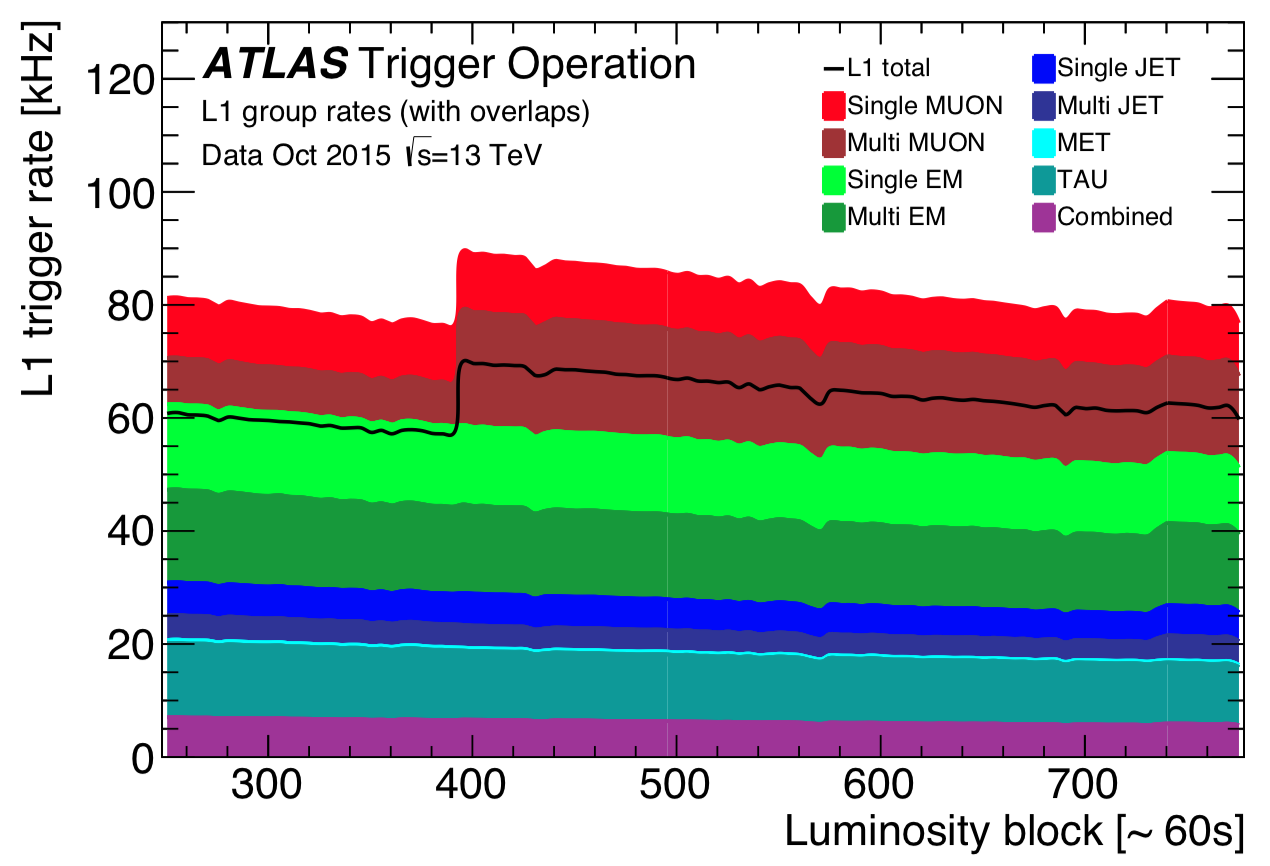
\includegraphics[width=0.75\textwidth]{fig/content_menu_figures_Time_L1GroupRate_Stack.png}
   \caption{}
  \label{fig:L1_menu_rates}
  \end{subfigure}
 \begin{subfigure}[b]{\textwidth}
 \centering
  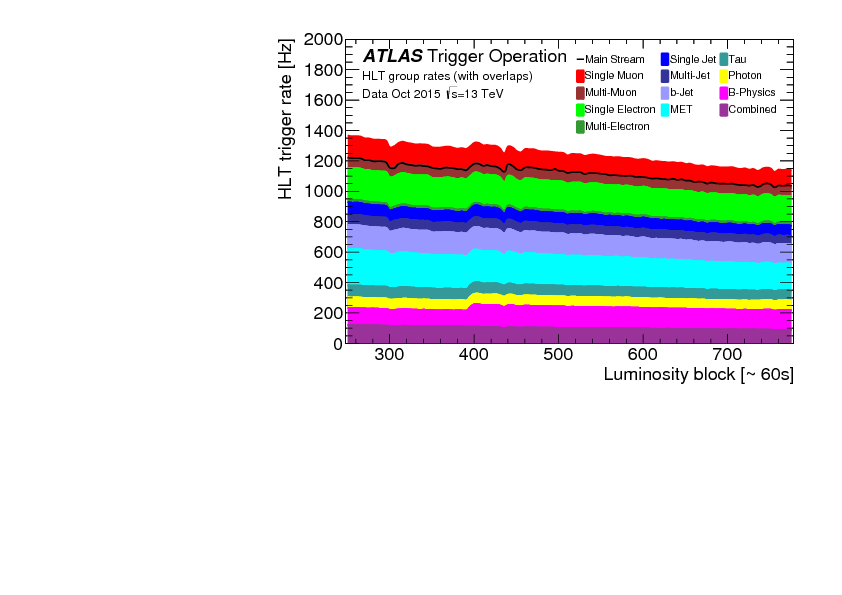
\includegraphics[width=0.75\textwidth]{fig/content_menu_figures_Time_HLTGroupRate_Stack.png}
   \caption{}
   \label{fig:HLT_menu_rates}
  \end{subfigure}
\caption{2015年LHC一次注入(fill)时的L1(a)和HLT(b)的各种信号组的触发率,此次注入最高亮度为$4.5\times10^{33}\text{cm}^{-2}\text{s}^{-1}$。因为各种信号类别之间有重叠,所以他们的触发率之和高于总的触发率(黑色实线),Multi-object触发项包含在b-jets与tau信号组中。亮度区间400之后的触发率增长是因为移除了B-physics prescaling。Combined触发组包含不同的触发信号,比如电子与$\mu$子, $\tau$, jets或者MET。\cite{Aaboud2017}} \label{fig:Trigger_singlelepton}
\end{center}
\end{figure}

\section{ATLAS Phase-II升级}
LHC在2020之后会进行一个主要升级,称为High Luminosity LHC(HL-LHC)其将在14 TeV能量下运行,瞬时亮度将达到原始设计目标的5倍$7.5\times10^{34}~\text{cm}^{-2}s^{-1}$,
LHC的计划运行和升级时间表可见图\ref{fig:LHC_timeline}。
HL-LHC的成功运行依赖于超导磁铁等新技术的运用,具体可见HL-LHC技术设计报告\cite{Apollinari:2284929}。
\begin{figure}[h]
\centering
 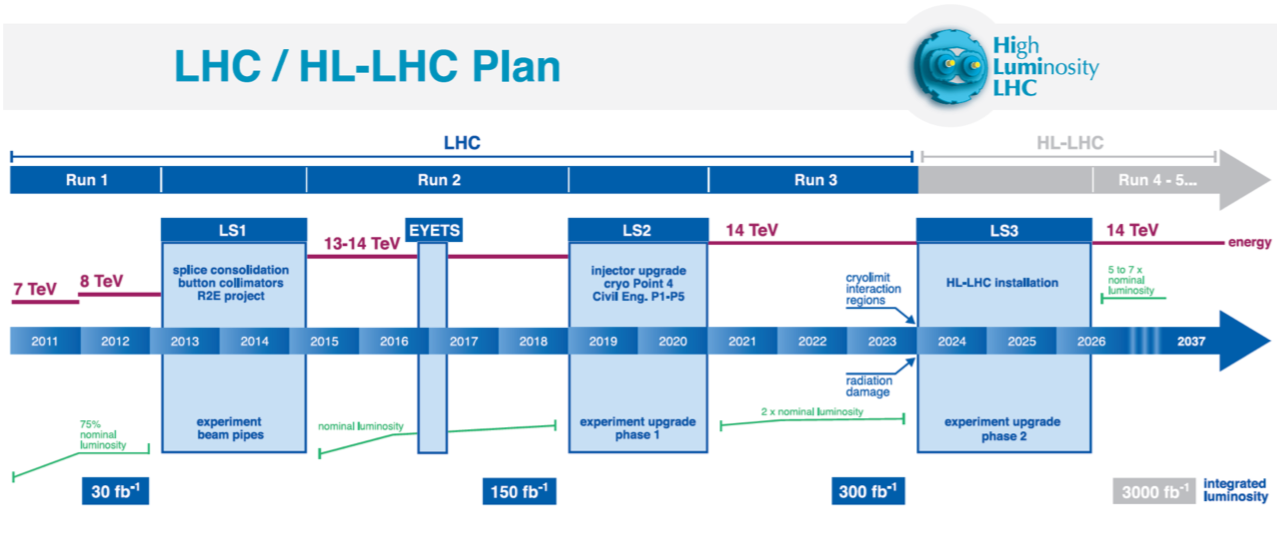
\includegraphics[width=0.85\textwidth]{fig/HL-LHC-PLAN.png}
 \caption{LHC运行和升级时间表\cite{Apollinari:2284929}。}
 \label{fig:LHC_timeline}
\end{figure}
为了承受HL-LHC的高\pileup 和高辐照压力,ATLAS探测器将进行一个全面升级。内部径迹探测器将全部替换成由硅组成的Inner Tracker(ITk),
ITk分为靠近束流的像素探测器(Pixel)\cite{Collaboration:2285585}和扩展到高半径的硅微条探测器(Strips)\cite{Collaboration:2017mtb},Pixel桶部区有五层,Strips则有四层,
一系列环形探测器也会添加到前向区使得寻迹区域扩展到$\abseta<4.0$。
Liquid Argon(LAr)量能器\cite{Collaboration:2285582}将会有全新的前端和读出电子学器件,其电子学架构设计在40 MHz输出全粒度数字信号(full-granularity digitized signals)。
Tile量能器\cite{Collaboration:2285583}会使用新的前端和读出电子学器件,电源和光链路接口板(optical link interface boards)。
$\mu$子探测器\cite{Collaboration:2285580}的一大部分前端,在和不在探测器(on- and off-detector)的读出和触发电子学设备将会被替换,额外的$\mu$子室也会安装以保持$\mu$子的鉴别和重建性能,
另外目前正在研究扩展到$\abseta<4.0$的可能性。
全新的触发和数据接收系统\cite{Collaboration:2285584}也会应用在升级ATLAS上。
考虑到HL-LHC的高pileup,一个新的探测器High-Granularity Timing Detector(HGTD)\cite{Collaboration:2623663}会安装在LAr量能器之前,覆盖$2.4<\abseta<4.0$区域,它可以精确测量带电粒子的时间分辨。
本章将关注硅微条探测器模块和ITk的预期寻迹性能研究。

\subsection{Strips模块组装及测试}
ATLAS Phase-II升级之后的硅微条探测器传感器覆盖165 m$^2$,桶部区有四层,而端部磁盘区有6层,总共需要建造18,000个基本探测模块(module)。一个完整模块由一个
硅传感器,两块或一块包含读出芯片(ABC130Star chip)以及控制芯片(HCCStar)的支撑电路板(hybrid)和电源控制模块(Power Board)组成,具体可见图\ref{fig:strips_module}.
虽然Strips硅传感器的大小和形状根据模块在探测器的位置决定(见图\ref{fig:strip_sensor_overview}),但是其整体设计和架构是一致的。读出芯片是二元设计(binary design),与每条strip通过
金属线相连,信号通过芯片初步处理之后传输到控制芯片,然后统一输出到读出系统,控制芯片同时负责传输控制命令,而电源控制模块则是用来控制整个模块的电源开关以及监控环境参数,各部分的具体
信息可见设计报告\cite{Collaboration:2017mtb}。本文将呈现整个模块的组装过程以及测试结果,所使用的芯片和控制芯片分别称为ABC130和HCC,具体区别同样可见\cite{Collaboration:2017mtb}。

\begin{figure}[h]
\centering
 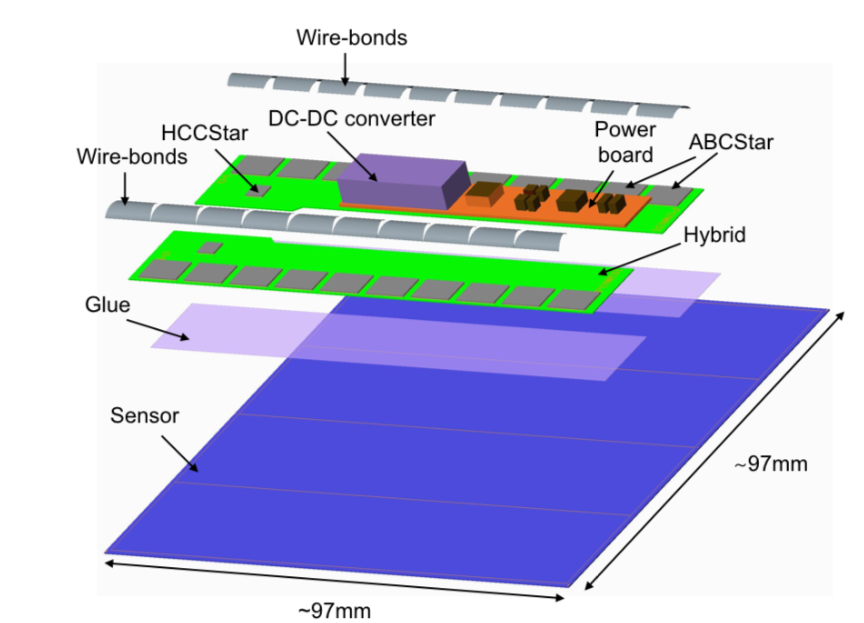
\includegraphics[width=0.85\textwidth]{fig/strips_module_3d.png}
 \caption{(short-strip)Strips模块。}
 \label{fig:strips_module}
\end{figure}

\begin{figure}[h]
\centering
 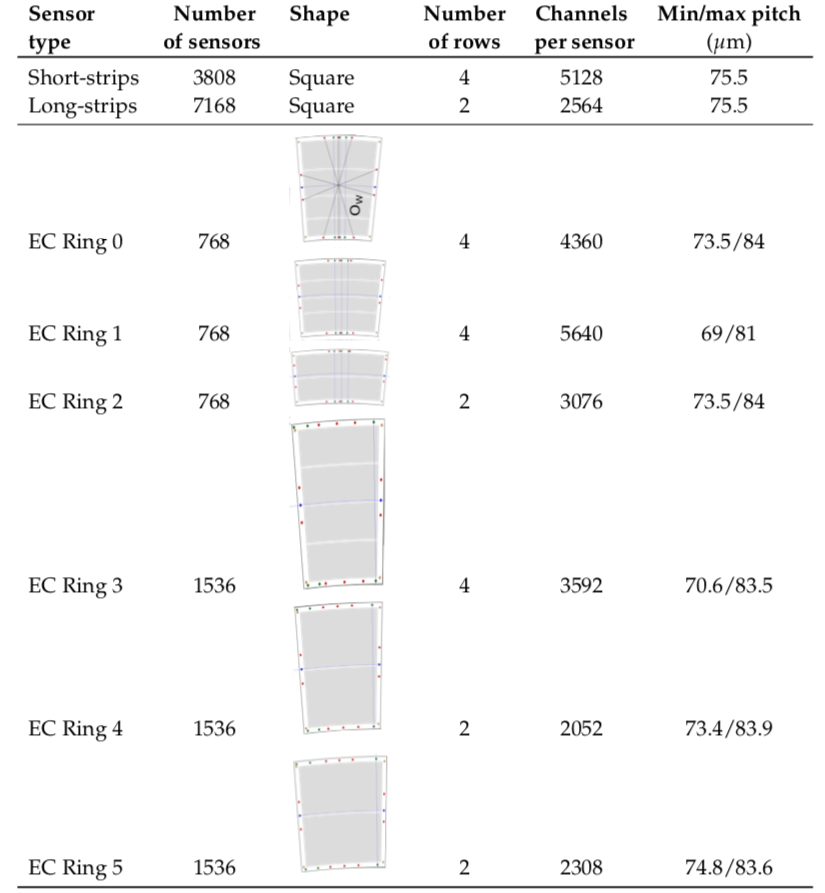
\includegraphics[width=0.85\textwidth]{fig/strips_sensor_overview.png}
 \caption{ITk Strips传感器种类\cite{Collaboration:2017mtb},Strips探测器桶部区内两层由短条(short-strip)传感器组成,外两层由长条(long-strip)组成,由于端部的扇形几何结构,其strip间距(pitch)随半径不同而不同。}
 \label{fig:strip_sensor_overview}
\end{figure}
模块的组装是探测器建造的重要一环,模块的质量决定了最终探测器的性能。
组装过程大致可以分为以下几步:
\begin{enumerate}
 \item 将读出芯片通过胶水粘合在hybrid的相应位置,而后连接读出芯片与hybrid(wire-bonding);
 \item 将芯片通过胶水粘合在传感器上,而后将每条strip与读出芯片相连;
 \item 最后粘合电源控制模块到传感器上,最后进行wire-bonding。
\end{enumerate}
其实际对应过程可见图片\ref{fig:strip_moduel_assembly}\footnote{过程中的具体粘合方法,所使用的器械以及工艺等,一直在进行优化,不同组装地点也可能使用不同的方法。}。
组装的挑战在于各个部分的接触面大小,胶水厚度以及位置的精确控制,一般要求控制到$\mathcal{O}(10)~\mu\text{m}$水平,比如芯片与hybrid的胶水粘合面应当保证至少50\%的接触面,
以便传导芯片工作时产生的大量热量,而固化的胶水应当保持在120$\pm40~\mu\text{m}$厚度。
\begin{figure}[h]
\centering
 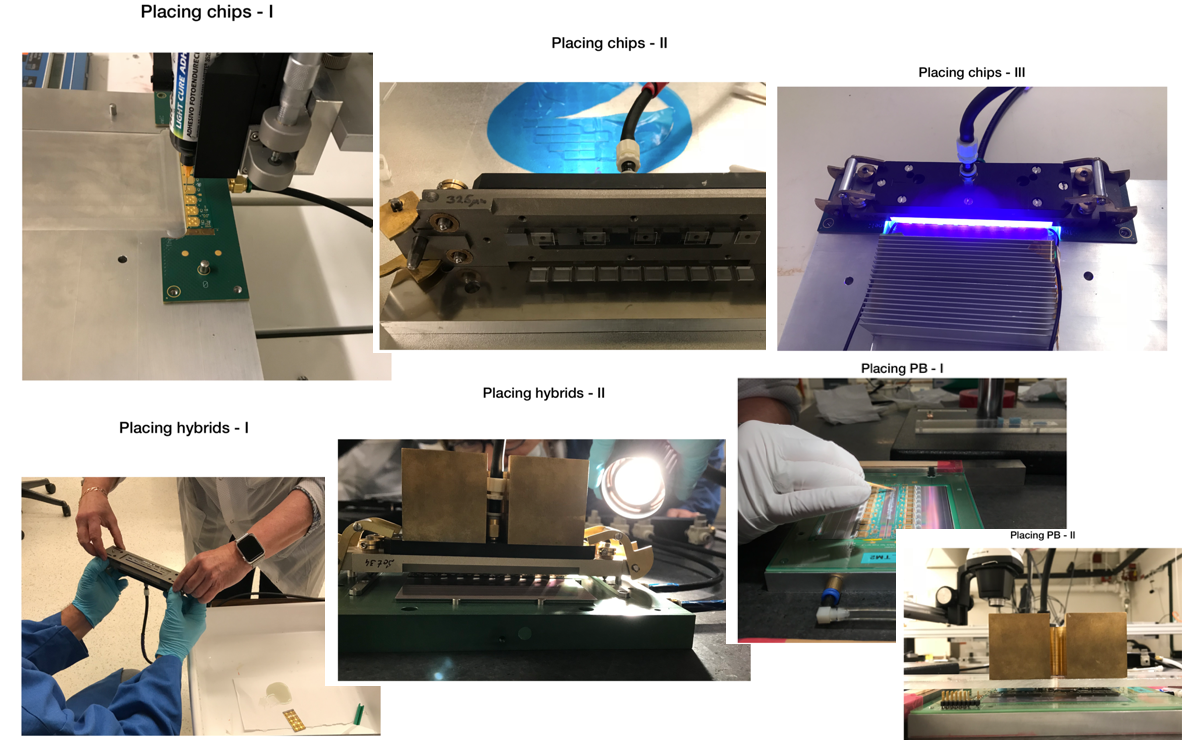
\includegraphics[width=0.85\textwidth]{fig/strips_module_assembly.png}
 \caption{ITk (short-strip)模块实际组装过程(省略wire-bonding过程),粘合芯片的胶水需要紫外线照射固化。}
 \label{fig:strip_moduel_assembly}
\end{figure}
组装完成的模块需要进行电子学测试,以保证模块工作性能达到预期。测试时,模块应当处于干燥且低温的环境中,其测试系统如图\ref{fig:strips_testing_setup}所示。
一个重要指标是衡量ABC130芯片的输入噪声(input noise),它由芯片本身和与之相连的strip噪声决定。
其测试基本原理是给定注入电荷,进行阈值扫描,确定输入噪声水平。图\ref{fig:strips_testing_noise}展示
几个模块粘合PB之前和之后的输入噪声水平,基本在600电子与900电子之间(模块经受辐照之后,整体噪声会上升)。图\ref{fig:strips_bad_dist}则为测试模块的
工作不良strip的空间分布。总体而言,所示的组装模块均工作良好,达到预期。
\begin{figure}[h]
\centering
 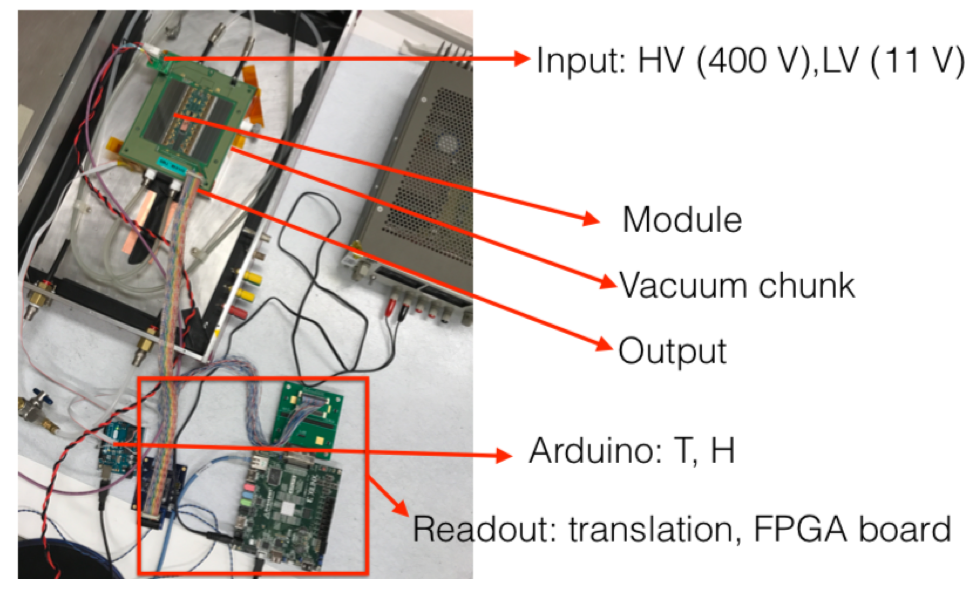
\includegraphics[width=0.85\textwidth]{fig/strips_module_setup.png}
 \caption{Strips模块测试系统设置。}
 \label{fig:strips_testing_setup}
\end{figure}
\begin{figure}[h]
\centering
 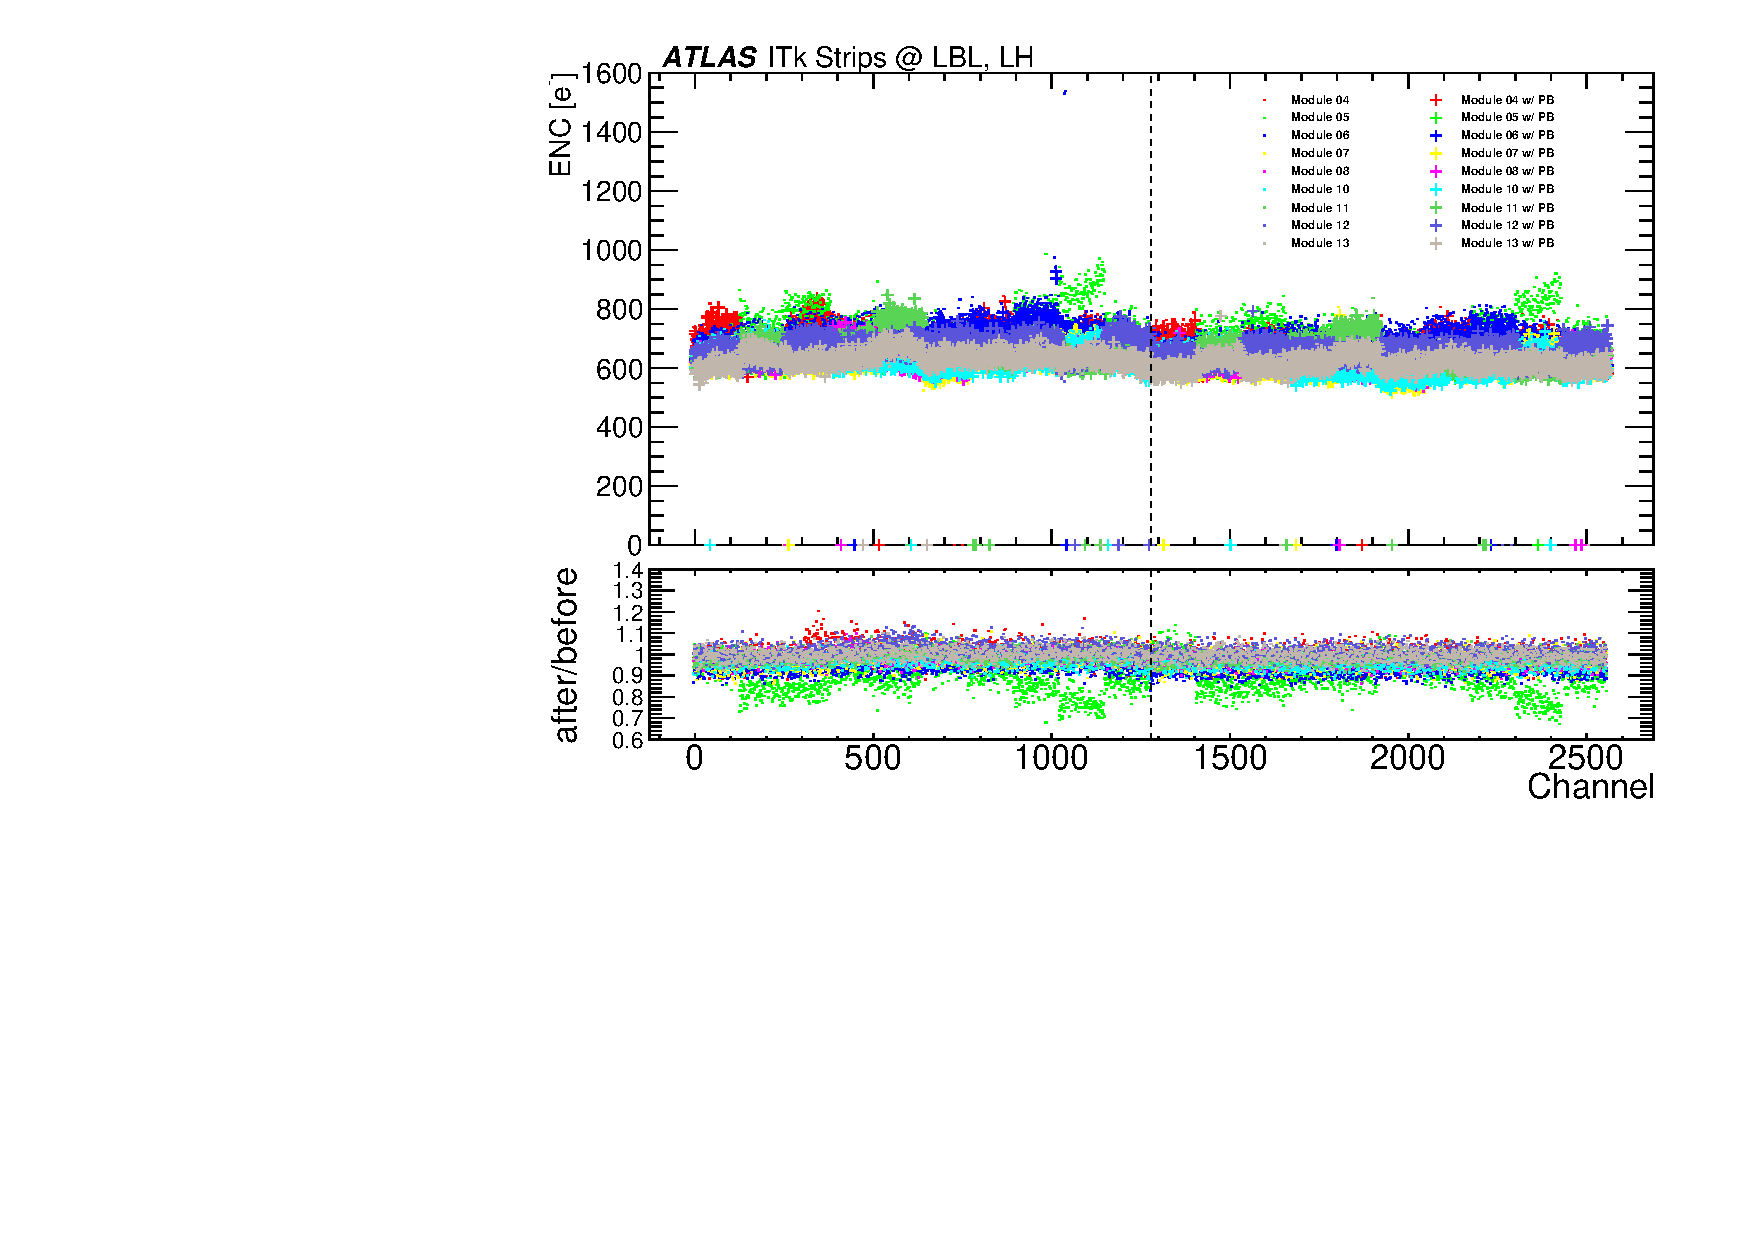
\includegraphics[width=0.65\textwidth, angle=-90]{fig/LH_noise.pdf} \\
  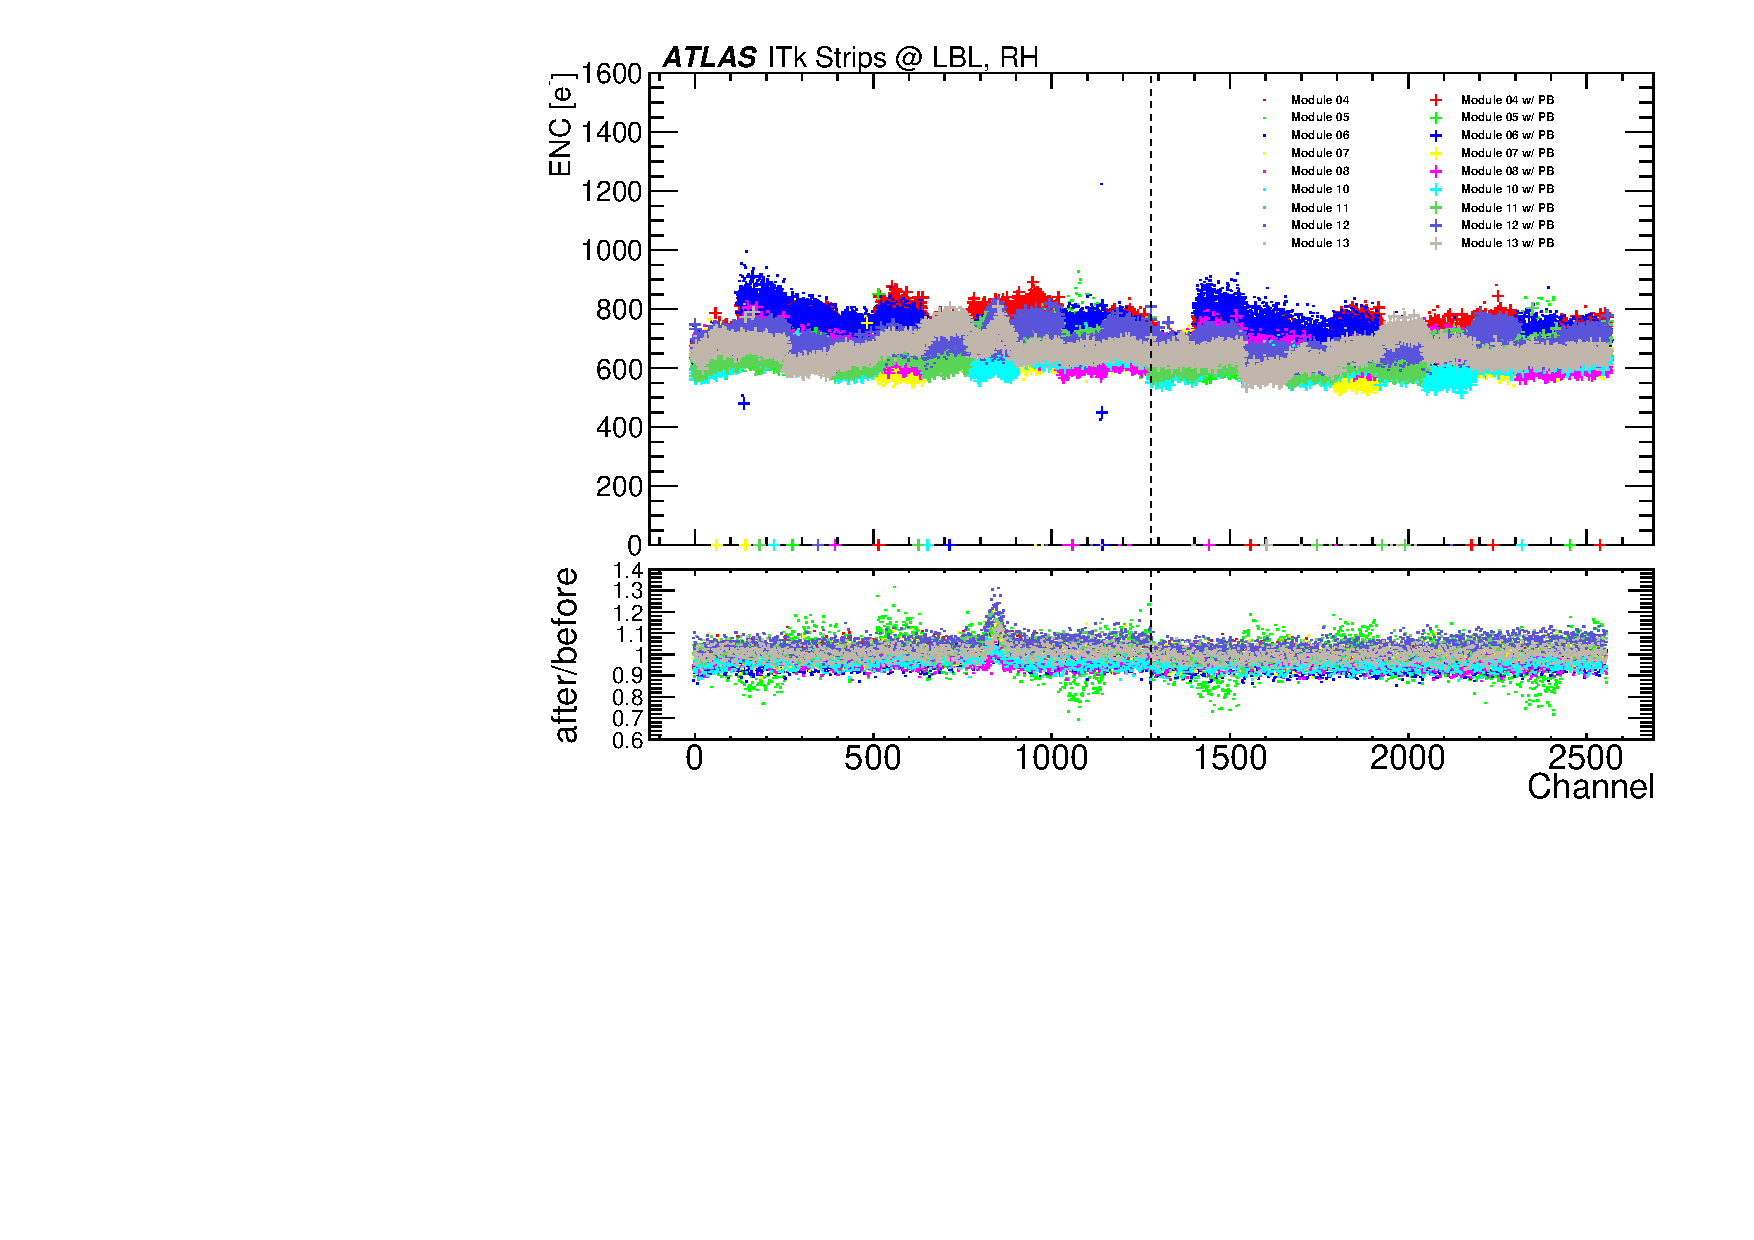
\includegraphics[width=0.65\textwidth, angle=-90]{fig/RH_noise.pdf} 
 \caption{Strips模块输入噪声,上图对应左手Hybrid (LH),下图对应右手Hybrid (RH), 点线为粘合PB之前,'+'为粘合PB之后,每图底部为粘合PB之后与之前的噪声之比。
 总体上比例在1附近,但因为每次实际测试时,环境参数并不一致,所以不能够表明粘合PB之后噪声一定增加或者减少了。}
 \label{fig:strips_testing_noise}
\end{figure}
\begin{figure}[h]
\centering
\begin{subfigure}[b]{0.45\textwidth}
\centering
 \includegraphics[width=0.9\textwidth,angle=-90]{fig/Hists_Bad_wPB.pdf}
 \caption{}
\end{subfigure}
\begin{subfigure}[b]{0.45\textwidth}
\centering
 \includegraphics[width=0.9\textwidth,angle=-90]{fig/BadDistr_LBL-EL-08_wPB.pdf}
 \caption{}
\end{subfigure}
\caption{(a)为测试模块strip整体不良率;(b)为LBL-EL-08模块不良strip在传感器上的分布情况。}
\label{fig:strips_bad_dist}
\end{figure}

\subsection{ITk预期寻迹性能}
相比目前的内部径迹探测器,ITk具有更低的物质量\footnote{目前研究显示材料预算在TDR被低估,这些预期结果也许过于乐观,全新的估计正在进行。},其具有更高的寻迹效率和分辨。
径迹重建从种子(seed)开始,所谓的seed是三个空间点。
在ITk的前期研究中,只考虑了两种seed,全部由Pixel着火点组成的PPP,全部由Strips着火点组成的SSS。
图\ref{fig:ITk_seeds}展示seeds随\abseta 分布,整体而言,PPP比SSS数目高一个量级。
联合拟合PPP与SSS,并消除掉重复着火点,同时满足一系列条件,即得到最终的径迹。
图\ref{fig:ITk_tracking_eff}展示径迹重建效率随$\eta$分布,可达90\%。
值得一提的是,由于径迹重建性能的提高,相比于\RunTwo ,电子电荷误判率下降,见图\ref{fig:ITk_ele_qmisid}。
\begin{figure}[h]
\centering
 \includegraphics[width=0.85\textwidth]{fig/ITk_seeds.png}
 \caption{ITk seeds随\abseta 分布%\footnote{在ITk研究前期,有两种布局,最后选用Inclined作为baseline}
\cite{seeds_ITk}。}
 \label{fig:ITk_seeds}
\end{figure}
\begin{figure}[h]
\centering
\begin{subfigure}[b]{0.45\textwidth}
\centering
 \includegraphics[width=0.9\textwidth]{fig/ITk_tracking_eff_tt.png}
 \caption{}
\end{subfigure}
\begin{subfigure}[b]{0.45\textwidth}
\centering
 \includegraphics[width=0.9\textwidth]{fig/ITk_tracking_eff_ratio.png}
 \caption{}
\end{subfigure}
\caption{(a) 径迹重建效率随$\eta$分布(matching criteria);(b) 重建径迹与真实粒子之比随$\eta$分布(no matching criteria)。\cite{ATL-PHYS-PUB-2016-025}}
\label{fig:ITk_tracking_eff}
\end{figure}
\begin{figure}[h]
\centering
\begin{subfigure}[b]{0.45\textwidth}
\centering
 \includegraphics[width=0.9\textwidth]{fig/ITk_ele_qmisid1.png}
 \caption{}
\end{subfigure}
\begin{subfigure}[b]{0.45\textwidth}
\centering
 \includegraphics[width=0.9\textwidth]{fig/ITk_ele_qmisid2.png}
 \caption{}
\end{subfigure}
\caption{(a) 不同工作点的电子鉴别效率随\et 分布;(b)电子电荷误判率随\abseta 分布。\cite{ATL-PHYS-PUB-2019-005}}
\label{fig:ITk_ele_qmisid}
\end{figure}


\section{事例重建}\label{sec:evt_reco}
重建是指将探测器各个子系统的着火点或者能量沉积的低级信息转换成与对撞中产生的粒子相关的高级信息的过程。
ATLAS中的重建是一个由集中式软件框架中的众多算法执行的复杂的多步骤过程\cite{Calafiura:2005zz},其最终输出是用于各种物理分析的物理对象(也简称为“对象”),包括电子,光子,$\mu$子,喷注和强子$\tau$候选者,以及MET。 下面将概述重建这些物理对象的基本步骤,更多地关注与本文中$hh$和$t\bar{t}h$搜索相关的对象。

\subsection{径迹和能量簇射}
重建的基本输入是径迹和能量簇射。

径迹是由带电粒子经过ID或者MS造成的一系列着火点构成的。
径迹重建\cite{Cornelissen:1020106}的初始种子是探测器(Pixel和SCT)中的三个空间着火点。
它们通过组合迭代算法形成径迹候选者,随后拟合到螺旋轨迹\cite{Cornelissen_2008},同时需要考虑材料效应,能量损失和多次散射以及磁场非均匀性。
然后通过根据每个候选者的属性(例如重合测量数量和拟合质量)对轨迹进行排序来解决模糊性。 最后轨迹被外推到TRT,并且在完整轨迹上执行新的拟合。
然后基于重建径迹使用专业算法\cite{Piacquadio_2008}决定每个束团对撞的顶点候选者,以及可用于识别重味喷注的次级顶点。

$\mu$子候选者的径迹通过连接ID中的轨迹与MS重建的轨迹得到。MS轨道搜索算法\cite{Benekos_2008}首先搜索精密室中的命中模式,以在每层中形成直线轨道段;
然后通过片段种子组合算法找到$\mu$子MS径迹候选者,并且根据全局$\chi^{2}$拟合得分接受或拒绝与每个候选者相关联的着火点。

来自量能器的能量簇射是ATLAS中粒子重建的另一个基本输入。 
穿过量能器的电子,光子和强子与活性材料相互作用而失去能量,并在纵向和横向上留下几个量能器单元的信号。 来自电子和光子的簇射主要包含在EM量能器中,而强子通常在HCal中产生簇射。
簇射算法\cite{Lampl:1099735}将着火单元组合在一起,根据粒子种类使用不同的逻辑,并将每个簇射内的总沉积能量相加,同时确定位置。根据进入的粒子类型(电子和光子,或强子射流),校准能量以补偿簇射外或者死区的能量沉积。

结合径迹和量能器簇射信息最终可以鉴别物理对象,图~\ref{fig:particle_id_patterns}显示ATLAS不同粒子的径迹和能量沉积模式。
\begin{figure}
\centering
\includegraphics[width=0.75\textwidth]{fig/particle_ID_patterns.png}
\caption{不同粒子在ATLAS探测器($r-\phi$平面)的径迹和能量沉积情况。}
\label{fig:particle_id_patterns}
\end{figure}

\subsection{电子}
电子和光子在EM量能器中有非常相似的特征。两个对象之间的主要区别在于电子也会在ID中留下径迹。ATLAS有许多基于光子末态的物理分析,因为它们具有非常好的能量分辨率。然而,本文分析并没有涉及光子,所以不述光子鉴别,光子重建的细节可以在参考文献\cite{ATLAS-CONF-2012-123}中找到。

对于电子,其簇射通过滑动窗口算法进行\cite{Lampl:1099735},即在一定范围内搜索使3$\times$5单元窗口(单元大小为0.025$\times$0.025,$\eta\times\phi$)内具有最大沉积能量并将其作为初始簇射种子,
即塔(tower\footnote{
%A tower in the EM calorimeter represents the set of cells contained in a 0.025$\times$0.025 ($\eta,\phi$)unit spanning longitudinally over the 3(4) calorimeter layers.
代表一系列着火单元,形状如塔。
}),
电子径迹重建如前面讲述,但考虑到电子通过ID时因韧致辐射造成的稍大的能量损失,会使用特定的模式识别和拟合假设。
使用高斯和滤波器(Gaussian Sum Filter)\cite{ATLAS-CONF-2012-047}重新拟合在$(\eta,\phi)$平面与EM簇射松散匹配的电子轨迹,以更好地考虑致辐射过程中的非线性。 然后在更严格的条件下匹配重新拟合后的轨迹与簇射,例如要求一定的最小硅着火点数以及在最内层Pixel中存在着火点以排除在ID中转换的光子。 电子能量由EM簇射给出,其最终校准基于蒙特卡罗模拟\cite{Aad2014-cali},而$\eta$和$\phi$坐标由相应的轨道参数给出。

电子重建仅针对$\abseta<2.47$和$\et >$7 GeV,对于$\pt>$15 GeV电子,重建效率大概在97\%到99\%。重建效率的测量基于$Z\rightarrow ee$和$J/\Psi\rightarrow ee$事例\cite{ATLAS-CONF-2016-024},其结果如图\ref{fig:ele_reco_eff}所示,数据和模拟样本中的效率差别在$\mathcal{O}(1)\%$水平,而且在实际分析中此相对差别会作为修正因子考虑到MC中。
\begin{figure}[h]
\begin{center}
\begin{subfigure}[b]{0.45\textwidth}
\centering
      \includegraphics[width=\textwidth]{fig/ele_reco_eff.png}
     \caption{}
      \label{fig:ele_reco_pt_eff}
  \end{subfigure}
 \begin{subfigure}[b]{0.45\textwidth}
 \centering
      \includegraphics[width=\textwidth]{fig/ele_reco_eta_eff.png}
      \caption{}
      \label{fig:ele_reco_eta_eff}
  \end{subfigure}
\caption{2105年数据与$Z\rightarrow ee$~MC中的电子重建效率随簇射\et (a)和簇射$\eta$ (b)分布情况\cite{ATLAS-CONF-2016-024}。} 
 \label{fig:ele_reco_eff}
\end{center}
\end{figure}

电子鉴别(\texttt{ID})通过基于似然函数多变量判别式\cite{ATLAS-CONF-2016-024}进行。算法的输入变量包括量能器簇射形状,基于TRT穿越辐射的似然概率和轨道-簇射匹配相关量,以及轨迹的测量总数和IBL中的测量数量和韧致辐射变量。
基于不同鉴别效率,定义三个电子鉴别工作点,分别命名为\texttt{Loose}, \texttt{Medium}和\texttt{Tight}。对于\et =25 GeV真实电子而言,它们的鉴别效率在78-90\%,而相应的本底误判率为0.3-0.8\%。
图\ref{fig:ele_id_eff_pileup}展示各个工作点随pileup数的变化情况,基本上其效率比较稳定。
\begin{figure}
\centering
\includegraphics[width=0.65\textwidth]{fig/ele_id_eff_pileup.png}
\caption{2015年数据和$Z\rightarrow ee$~MC在不同工作点的鉴别效率随顶点数分布情况\cite{ATLAS-CONF-2016-024},背景中的灰色直方图为顶点数的分布情况。}
\label{fig:ele_id_eff_pileup}
\end{figure}

$Z\rightarrow ee$和$J/\Psi\rightarrow ee$事例也用来测量触发效率\cite{ATLAS-CONF-2016-024}。图\ref{fig:ele_trigger_eff}展示2015年使用的单电子触发器\footnote{\texttt{HLT\_e24\_lhmedium\_L1EM20VH}}效率随\et 和$\eta$ 的变化,在$\et>$27 GeV时,触发效率
可达95\%,数据与MC之间的差别在5\%以内。最大的偏差发生在24 GeV附近,这是因为在L1阶段,数据与MC使用了不同的阈值,MC会根据这些差别进行修正。
\begin{figure}[h]
\begin{center}
\begin{subfigure}[b]{0.45\textwidth}
\centering
      \includegraphics[width=\textwidth]{fig/ele_trigger_eff_et.png}
     \caption{}
      \label{fig:ele_trigger_et_eff}
  \end{subfigure}
 \begin{subfigure}[b]{0.45\textwidth}
 \centering
      \includegraphics[width=\textwidth]{fig/ele_trigger_eff_eta.png}
      \caption{}
      \label{fig:ele_trigger_eta_eff}
  \end{subfigure}
\caption{2015年电子和$Z\rightarrow ee$~MC的单电子触发效率随\et~(a)和$\eta$~(b)的分布情况\cite{ATLAS-CONF-2016-024}。} 
 \label{fig:ele_trigger_eff}
\end{center}
\end{figure}

\subsection{$\mu$子}
$\mu$子重建联合利用ID和MS的径迹,以及量能器信息,它有四类:
\begin{itemize}
 \item Combined muons (CB). 这些$\mu$子通过同时拟合ID和MS的着火点得到,在拟合过程中,MS着火点可以被添加或者移除已改善拟合质量。
 \item Segment tagged muons (ST). 这类$\mu$子代表当完整ID轨迹仅与MDT或CSC中的一个轨道段(segment)匹配时的情况,这要么是因为\pt 低或者因为它们穿过MS接收度低的区域。
 \item Calorimeter tagged muons (CT). 来自电弱衰变的高动量$\mu$子在穿过量能器时仅沉积很少的能量,与最小的电离损失相当。当ID轨迹与一个这样的簇射匹配时,则定义为CT~$\mu$子候选者。 
 这些$\mu$子是假的概率较高,但可以在MS探测器件较少的$\abseta<0.1$区找回一些。
 \item Extrapolated muons (ME). 为了处理ID未覆盖的前向区$2.5<\abseta<2.7$,可以仅重建MS的轨迹,然后考虑在量能器内的能量损失后外推回初级顶点。
\end{itemize}
不同类别的$\mu$子重叠消除之后,才定义物理分析可用的对象粒子。值得指出的是,$\mu$子重建可到4 GeV。与电子类似,有三个$\mu$子质量工作点:\texttt{Loose}, \texttt{Medium}和\texttt{Tight}。
\texttt{Tight}~$\mu$子仅包括CB类,并且有额外的径迹质量要求以压低不是来自初级顶点的$\mu$子;\texttt{Medium}~$\mu$子也包括$\abseta>2.5$的ME类,但是要求至少存在要个MS径迹segment;
\texttt{Loose}~$\mu$子也包括ST和CT类。

$\mu$子重建效率的评估与电子类似,利用$Z\rightarrow \mu\mu$和$J/\Psi\rightarrow \mu\mu$事例\cite{Aad2016-mu2016}。对于\texttt{Loose}类和\texttt{Medium}类,重建效率为98\%,而对于\texttt{Tight}类,平均为95\%。图\ref{fig:muon_reco_eff}总结2016年$\mu$子重建效率情况,可以看到,数据与MC的差别在几个百分点,主要集中在MDT对齐稍差的桶部区。
\begin{figure}[h]
\begin{center}
\begin{subfigure}[b]{0.45\textwidth}
\centering
      \includegraphics[width=\textwidth]{fig/muon_reco_eff_pt.png}
     \caption{}
      \label{fig:muon_reco_eff_pt}
  \end{subfigure}
 \begin{subfigure}[b]{0.45\textwidth}
 \centering
      \includegraphics[width=\textwidth]{fig/muon_reco_eff_eta.png}
      \caption{}
      \label{fig:muon_reco_eff_eta}
  \end{subfigure}
\caption{2015+2016年数据与$Z\rightarrow \mu\mu$,  $J/\Psi\rightarrow \mu\mu$~MC中的$\mu$子重建效率随\pT~(a)和$\eta$~(b)分布情况,(b)中$\abseta<0.1$区间\texttt{Loose}~$\mu$子效率
的回升是因为使用calorimeter-tagged的$\mu$子定义。} 
 \label{fig:muon_reco_eff}
\end{center}
\end{figure}

$\mu$子触发效率\cite{Muon-trigger-results}表现估计与电子类似。图~\ref{fig:muon_trigger_eff}展示L1 MU20触发器的效率,这类触发要求MS中至少存在一个$\pt>$20 GeV的$\mu$子候选者。
L1桶部触发效率大约为70\%,而在前向区为90\%,这是因为RPC比TGC更少的几何接收度。然而对于通过L1的$\mu$子,HLT触发效率可达100\%。数据与MC之间的触发效率相差在几个百分比水平。
\begin{figure}[h]
\begin{center}
\begin{subfigure}[b]{0.45\textwidth}
\centering
      \includegraphics[width=0.7\textwidth,angle=-90]{fig/HLT_mu26_ivarmedium_OR_HLT_mu50_Medium_IsoFixedCutTightTrackOnly_barrel_probe_pt_eff.pdf}
     \caption{}
      \label{fig:muon_trigger_eff_pt_barrel}
  \end{subfigure}
 \begin{subfigure}[b]{0.45\textwidth}
 \centering
      \includegraphics[width=0.7\textwidth,angle=-90]{fig/HLT_mu26_ivarmedium_OR_HLT_mu50_Medium_IsoFixedCutTightTrackOnly_endcap_probe_pt_eff.pdf}
      \caption{}
      \label{fig:muon_trigger_eff_pt_endcap}
  \end{subfigure}
\caption{2015+2016年数据中L1 MU20 seed的触发效率随\pT~分布\cite{Muon-trigger-results},HLT的在线筛选对$\mu$子有一定的isolation要求。}
%The online selection at HLT includes a requirement of low activity around the muon candidate (isolation).} 
 \label{fig:muon_trigger_eff}
\end{center}
\end{figure}
MC中$\mu$子动量大小和分辨率会根据对撞数据校准\cite{Aad2016-mu2016},其相对分辨率在1.7\%与2.9\%之间,在校准之后,对于大部分\abseta 区域数据与MC的分辨率相差在5\%以内。

\subsection{喷注}\label{subsec:jet_reco}
硬散射过程中的末态夸克和胶子(也包括初态辐射)会通过虚胶子的微扰辐射产生部分子簇射,当簇射能量传递下降到典型的强子尺度$\Lambda_{\text{QCD}}\approx$200 MeV时,%?
QCD微扰论不再适用,强子化过程开始,即形成无色荷的束缚态。

从探测器角度看,强子化的结果是一束相互比较靠近的强子,被称为喷注(jet),显然,喷注的能量和方向是与初始部分子直接相关的。
ATLAS喷注重建算法的输入是相邻的着火单元簇射(topoclusters)\cite{Aad:2016upy}。
%在本文物理分析中使用的喷注是由在电磁能量标度(EM)下校准的topoclusters构建的,
%它正确地测量了量能器中电磁簇射的沉积能量\cite{ATLAS-CONF-2013-004}。
本文使用的喷注是由在电磁能量标度(EM)下刻度的topoclusters构建的。

本文使用的喷注是利用\antikt 算法\cite{Cacciari:2008gp}在$\Delta R$=0.4范围基于topoclusters构建的,其($\pt>$25 GeV)能量大小和分辨最终通过仿真的技术校准到真实部分子能量,而且在data-driven中得到证实\cite{TheATLAScollaboration:2015soq,TheATLAScollaboration:2013pia}。

$\pt<$60 GeV, $\abseta<$2.4的喷注有一定概率的来自\pileup ,一个称为喷注顶点标记(JVT)\cite{ATLAS:2014cva}的算法通过关联喷注径迹与顶点可以压低\pileup 影响。在$t\bar{t}h$分析对
该算法的应用中,每个喷注的平均关联效率为92\%。JVT的效率利用$Z\rightarrow \mu\mu$+jets事例校准,最终的MC的修正因子在1-5\%之间。

顶夸克是标准模型中最重的粒子,不会强子化,几乎百分百衰变到$W+b$。来源于$b$夸克的喷注一般会包含$B^{\pm}$介子,而$B^{\pm}$介子衰变之前会经过一段宏观可探测到的距离($c\tau_{B^{\pm}}\approx0.5~\text{mm}$)。这个性质可以用来标记来源于$b$夸克的喷注,从而间接标记顶夸克。在ATLAS实际应用中,一个联合利用喷注径迹影响参数,次级顶点,
以及$b$或$c$强子衰变拓扑结构的多变量学习算法MV2\cite{ATL-PHYS-PUB-2015-022,ATL-PHYS-PUB-2016-012}开发出来用于标记$b$喷注。在本文的$hh$和$t\bar{t}h$分析中使用的是MV210,它的训练样本是$t\bar{t}$,并且假设本底是93\%轻
夸克喷注与7\%~$c$夸克喷注,所使用的工作点对应70\%~\btag 效率,以及对$c$喷注(轻味喷注)的排除因子(rejection factor)为12 (381)。
而后使用与\RunOne 类似的方法\cite{Aad:2015ydr}校准MC~\btag 效率到数据,基本上修正因子在5\%以内,最大的系统误差不超过10\%。

\subsection{$\tau_{\text{had}}$}
$\tau$轻子有较大的质量($\approx$1.77 GeV),而且不稳定,大约36\%衰变到电子或者$\mu$子,而剩下的64\%衰变到强子。对于强子化衰变的$\tau$子,标记为$\tau_{\text{had}}$,
主要有两类,一类是末态有一个带电$\pi$介子(1-prong),另一类是有三个带电$\pi$介子(3-prong)。
因为$\tau$轻子的衰变长度很短($c\tau\approx87\mu$m),非常靠近顶点,区分来源于$\tau$轻子与直接来源于顶点的电子或$\mu$子比较困难,而$\tau_{\text{had}}$
在ID中有1条或者3条径迹,并且相对准直的径迹与能量簇射使得重建比较可行。关于$\tau_{\text{had}}$的重建及鉴别可参见~\cite{ATL-PHYS-PUB-2015-045}。
$tt\bar{h}$分析中几个分析道都包含$\tau_{\text{had}}$末态,它可以用来压低QCD喷注本底。

\subsection{丢失横动量}\label{subsec:met_reco}
在横截面平面,总动量为零,那么可以定义丢失横动量如下:
\begin{equation}
\overrightarrow{E}_{T}^{miss}=\overrightarrow{E}_{x}^{miss}+\overrightarrow{E}_{y}^{miss}=-\sum \overrightarrow{E}_{T}^{vis}
\end{equation}
$\overrightarrow{E}_{T}^{miss}$包含不与探测器反应的中微子或者刚好穿过探测器死区的粒子。丢失横动量的大小定义为:
\begin{equation}
 \met=\sqrt{(E_x^{miss})^2+(E_y^{miss})^2}
\end{equation}
\begin{equation}\label{eq:E_miss_xy}
  E_{x(y)}^{miss}=-\sum E_{x(y)}^{vis}.
\end{equation}

ATLAS \met 重建算法\cite{Aaboud:2018tkc}会考虑所有校准之后的重建粒子作为方程\ref{eq:E_miss_xy}右端的输入,即:
\begin{equation}
\begin{aligned}
 E_{x(y)}^{miss}=E_{x(y)}^{miss,e}+E_{x(y)}^{miss,\gamma}+E_{x(y)}^{miss,\tau}+E_{x(y)}^{miss,jet}+\\
 E_{x(y)}^{miss,TST}+E_{x(y)}^{miss,\mu}
 \end{aligned}
\end{equation}
其中,TST (Track Soft Term)指ID中未与其他粒子重建联系起来的低动量径迹,需要指出的是,这一项也可以使用量能器中未被其他粒子重建使用的能量,但会导致\met 有很强的pileup 依赖。
\met 的重建表现可见\cite{Aaboud:2018tkc}

\section{事例仿真}\label{sec:evt_simulation}
%物理分析的一项重要目标是比较高能对撞的观测数据和某些假设或者预测模型,包括某些感兴趣的物理过程以及相应本底过程。
%通常情况下,可用的观测数据数量有限,不足以提供足够精度去描述需要的物理过程,尤其是当该物理过程截面本身很小时。
%所以,对标准模型物理过程以及新物理模型进行仿真是非常有必要的,可以提供大量的仿真事例用来理解与研究。
物理分析的一项重要目标是验证或排除理论预测,在对撞实验中,理论预测需要与观测数据进行比较,
为实现这一目的,需要对理论模型进行仿真。同时仿真事例也可用来理解本底组成和新信号运动学分布。

ATLAS的仿真是包括事例产生和探测器模拟的多步骤过程。
一个典型的质子质子-对撞过程如图~\ref{fig:evt_egen_chain}所示,一般关心的是携带大动量的部分子的碰撞,即硬散射过程,而后衰变,部分子簇射以及强子化得到稳定粒子,这些都通过蒙特卡罗事件产生子(Monte-Carlo generator)模拟\cite{BUCKLEY2011145}。最后,模拟稳定粒子与探测器的相互作用。
\begin{figure}
\centering
\includegraphics[width=0.75\textwidth]{fig/evt_egen_chain.png}
\caption{产生子中$t\bar{t}h$事例演化过程\cite{Gleisberg:2008ta}。首先携带大动量的硬散射过程发生(大红色圆),随后$t$和$h$衰变(小红色圆),衰变产物发生QCD硬辐射(红色);除硬散射之外,次要散射(由参与硬散射之外的部分子参与)也可能发生(紫色);最后辐射到一定低能量时,强子化过程发生(浅绿),强子化产物衰变到稳定粒子(深绿)。光子辐射可在任一阶段发生(黄色)。}
\label{fig:evt_egen_chain}
\end{figure}
\begin{itemize}
  \item 整合所仿真的物理过程的相空间(运动学,自旋),在一定的QCD或者QED微扰展开级数下计算并模拟硬散射过程(Matrix element)。
  \item 利用专用程序模拟硬散射过程的部分子的初态和末态辐射胶子以及紧接的部分子簇射过程(PS),在这一般是使用微扰QCD来模拟粒子级联,通常能到次级对数精度(NLL),这个过程直到微扰QCD不再
  适用的尺度$\Lambda_{\text{QCD}}\approx200$MeV才停止。类似PS,QED过程的辐射光子利用等价的数学框架模拟。
  \item 强子化过程不依赖于初始的物理过程,即Matrix element,它不能使用微扰QCD论,目前从第一性原理出发也未能理解,所以一般通过基于实验数据的唯象模型描述,所使用的方法
      在不同的软件环境中有不同的实现。
   \item 仿真\texttt{underlying event} (UE)。UE代表了碰撞质子中未参与硬散射过程的部分子的强子化,或者它们之间的相互作用,它们可以是微扰QCD尺度,也可以在非微扰尺度。同样地。
   导致\pileup 的\texttt{minimum bias}事件也会叠加在硬散射事例中。
   \item 利用GEANT4软件\cite{AGOSTINELLI2003250}模拟前面步骤产生的稳定粒子与探测器的相互作用,探测器的几何形状与材料分布都会考虑\cite{Aad2010-atlas-simu}。这个步骤是是整个ATLAS实验耗费计算资源最多的一环,
     所以对某些过程使用所谓的快速模拟技术(fast simulation)\cite{Lukas:2012kua}以节省计算资源和加快模拟过程。
    \item 探测器着火点被复现并数字化,而后进行与对撞数据完全一样的事例重建过程,并且以相同的文件格式存储。在这过程中,也对触发决策进行模拟。
 \end{itemize}

 如前所述,仿真样本的重建效率,鉴别效率,触发效率和能量刻度以及能量校准都会乘上一定的修正因子使之与真实数据匹配,需要注意的是,pileup仿真强烈依赖假设的对撞条件。

%\part{通过多轻子道寻找$t\bar{t}H$产生模式}
\chapter{通过多轻子道寻找$t\bar{t}h$产生模式}\label{chap:tth_multilep}
\section{$t\bar{t}h$发现}
目前ATLAS实验搜寻$t\bar{t}h$通过以下衰变道进行:
\begin{itemize}
 \item $t\bar{t}(h\rightarrow b\bar{b})$
 \item $t\bar{t}(h\rightarrow \gamma\gamma)$
 \item $t\bar{t}h\rightarrow$ 多轻子\footnote{本文称tthML}
\end{itemize}
$t\bar{t}(h\rightarrow b\bar{b})$具有最大的衰变分支比,其主要信号特征是很高的$b$喷注数。$t\bar{t}(h\rightarrow \gamma\gamma)$虽然衰变分支比很小,
但得益于双光子的良好的分辨,这个分析道有很好的希格斯质量极点和信号纯度。
tthML并不显性关注某个中间过程,它根据轻子数或者$\tau_{had}$数分类,主要针对$h\rightarrow WW^*$, $h\rightarrow \tau\tau$和$h\rightarrow ZZ^*$\footnote{不包括$t\bar{t}h\rightarrow ZZ^*\rightarrow 4\ell$},相应的数图阶费曼图见\ref{fig:diagram_tthML_LO}。
这种搜寻策略是因为我们的目标是确定$t\bar{t}h$的产生率,而不是耦合常数测量。在\RunOne ATLAS和CMS已通过以上衰变道进行$t\bar{t}h$寻找\cite{Aad:2015iha,Aad:2015gra,Aad:2014lma,Khachatryan:2014qaa,Khachatryan:2015ila,Khachatryan:2016vau},
联合ATLAS和CMS结果(图\ref{fig:HiggsPromu_ATALS_CMS})给出信号强度$\mu_{t\bar{t}h}=\sigma/\sigma_{SM}=2.3^{+0.7}_{-0.6}$,超出主要来自tthML测量,其结果为$\mu_{t\bar{t}h}=2.1^{+1.4}_{-1.2}$,95\%置信度下上限为$\mu_{t\bar{t}h}<4.7$,对应观测(期望)显著性为1.8$\sigma$(0.9$\sigma$)。

13 TeV~$t\bar{t}h$总截面相比8 TeV结果增加了3.9倍\cite{Heinemeyer:2013tqa,XSWG13TeV},
并且随着更多数据的累积,$\mu_{t\bar{t}h}$测量精度会得到显著提升。2017年ATLAS利用\RunTwo 36.1 fb$^{-1}$数据报告了$t\bar{t}h$存在证据\cite{Aaboud:2017jvq},联合以上衰变道给出观测(期望)显著性为4.2$\sigma$(3.8$\sigma$),$\mu_{t\bar{t}h}$的最佳拟合值为$1.2\pm0.2(\text{stat})^{+0.3}_{-0.2}(\text{syst})$,与标准模型预期基本一致,值得指出的是,tthML最敏感,其观测(期望)显著性为4.1$\sigma$(2.8$\sigma$)。
2018年ATLAS与CMS联合\RunOne 和\RunTwo 部分数据分别宣告发现$t\bar{t}h$\cite{Aaboud:2018urx,PhysRevLett.120.231801},
相应的信号强度测量结果ATLAS为$\mu_{t\bar{t}h}=1.32\pm0.18(\text{stat})^{0.21}_{-0.19}(\text{syst})$,CMS为$\mu_{t\bar{t}h}=1.26^{+0.31}_{-0.26}$
,其中ATLAS tthML给出$\mu_{t\bar{t}h}=1.56^{+0.30}_{-0.29}(\text{stat})^{0.30}_{-0.27}(\text{syst})$。
本章将叙述利用\RunTwo 2015-2017年数据进行的tthML分析,
主要关注\ltwotau 衰变道,并分别给出\ltwotau 拟合结果和tthML联合拟合结果。
\begin{figure}[h]
\centering
 \includegraphics[width=0.7\textwidth]{fig/diagram_tth_LO.png}
 \caption{tthML树图阶费曼图,左图:$h\rightarrow WW^*/ZZ^*$,右图:$h\rightarrow \tau\tau$。}
 \label{fig:diagram_tthML_LO}
\end{figure}

\begin{figure}[h]
\centering
 \includegraphics[width=0.7\textwidth]{fig/ATLAS_CMS_HiggsMes.png}
 \caption{Run 1联合ATLAS与CMS数据给出的希格斯产生模式最佳拟合值\cite{Khachatryan:2016vau},粗线表示1$\sigma$,细线表示2$\sigma$。}
 \label{fig:HiggsPromu_ATALS_CMS}
\end{figure}

\begin{figure}[h]
\centering
\begin{subfigure}[b]{0.95\textwidth}
\centering
 \includegraphics[width=0.75\textwidth]{fig/ATLAS_ttH_mu_80fb.jpg}
 \caption{ATLAS结果\cite{Aaboud:2018urx}}\label{subfig:ATLAS_tth_mu_80fb}
\end{subfigure}\\
\begin{subfigure}[b]{0.95\textwidth}
\centering
 \includegraphics[width=0.75\textwidth]{fig/CMS_ttH_mu_80fb.png}
 \caption{CMS结果\cite{PhysRevLett.120.231801}}\label{subfig:CMS_tth_mu_80fb}
\end{subfigure}
 \caption{Run 2 $t\bar{t}h$信号强度测量结果。}
 \label{fig:HiggsPromu_ATALS_CMS}
\end{figure}

\section{tthML分类}
为了最大限度利用tthML数据,tthML会根据轻子数或者$\tau_{had}$数分类,最后联合拟合所有分析道得到信号强度。对于2015-2017年数据分析,tthML有以下六个分析道(图\ref{fig:tthML_cates}):
\begin{itemize}
 \item $2\ell\text{SS}$:两个相同电荷轻子,并且没有$\tau_{\text{had}}$。
 \item $3\ell$:三个轻子,总电荷为$\pm1$,并且没有$\tau_{\text{had}}$。
 \item $4\ell$:四个轻子,总电荷为0。
 \item $2\ell\text{SS}+1\tau_{\text{had}}$:两个相同电荷轻子,一个$\tau_{\text{had}}$。
% \item $2\ell\text{SS}+2\tau_{\text{had}}$:两个相同电荷轻子,两个$\tau_{\text{had}}$。
 \item $3\ell+1\tau_{\text{had}}$:三个轻子,总电荷为$\pm1$,一个$\tau_{\text{had}}$。
 \item \ltwotau :一个轻子,两个相反电荷的$\tau_{\text{had}}$。
\end{itemize}
%相应的分类也可见图\ref{fig:tthML_cates}
\begin{figure}[h]
\centering
 \includegraphics[width=0.75\textwidth]{fig/tthML_cates.png}
 \caption{tthML分类图示。}
 \label{fig:tthML_cates}
\end{figure}
如图\ref{fig:tthML_signal_comp}所示,不同类别对不同希格斯衰变敏感,$2\ell\text{SS}$,$3\ell$以及$4\ell$~的80\%信号来自$h\rightarrow WW^*$,并且$3\ell$和$4\ell$的一部分信号为$h\rightarrow ZZ^*$,大约为5\%$\sim$10\%,还观察到随着$\tau_{had}$数增加,$h\rightarrow \tau\tau$贡献越大,其中\ltwotau ~98\%信号贡献是$h\rightarrow \tau\tau$,这是
\ltwotau 的独特之处。另外,$4\ell$信号纯度($S/B$)最高,但是受限于统计量,显著性($S/\sqrt{B}$)一般,最高显著性为$2\ell\text{SS}$和$3\ell$。
\begin{figure}[h]
\centering
 \includegraphics[width=0.85\textwidth]{fig/tthML_signal_comp.png}
 \caption{左图:tthML信号类别中希格斯衰变来源分布;右图:$S/B$(黑色),$S/\sqrt{B}$(红色)。其中'other'主要贡献来自$h\rightarrow \mu\mu$和$h\rightarrow b\bar{b}$。\cite{Aaboud:2017jvq}}
 \label{fig:tthML_signal_comp}
\end{figure}

\section{数据与MC}
本文tthML分析使用2015-2017年的对撞数据,总共80 fb$^{-1}$,具体收集情况可参见亮度章节\ref{fig:data_taking}。

表\ref{tab:mcconfig}总结信号与背景MC产生情况,所有希格斯粒子质量均设为125 GeV。\tth 通过\POWHEGBOX 产生,\ttz 通过\MGMCatNLO 在QCD次领头阶产生,两种样本而后
均使用\PYTHIA 8 模拟部分子簇射和强子化过程。单举\ttbar$\ell\ell$ 过程(包括\ttbar$\ell\ell$, \ttbar$\ell\ell+q/g$及\ttbar$\ell\ell+2q/g$)的硬散射模拟考虑了不在壳的$Z$玻色子和虚光子($\gamma^*$)贡献,要求$m(\ell\ell)>5$ GeV。$t\bar{t}W$ MC使用\textsc{Sherpa 2.2.5}产生,对于具有最多一个出射额外部分子事例在次领头阶计算,而对于其他事例在领头阶计算。
\tth 总截面为507.1 fb,在QCD次领头阶和使用电弱参数\cite{Beenakker:2001rj,Beenakker:2002nc,Dawson:2002tg,Dawson:2003zu,Yu:2014cka,Frixione:2014qaa,Frixione:2015zaa}计算得到\cite{Heinemeyer:2013tqa,XSWG13TeV},来自QCD重整化和因子化的误差为$^{+5.8\%}_{-9.2\%}$,来自PDF和$\alpha_s$的误差为$\pm3.6$\%。
$t\bar{t}V$(包括$pp\rightarrow t\bar{t}\ell^+\ell^-+X$)产生截面计算到QCD次领头阶\cite{Alwall:2014hca,Frixione:2015zaa},$\sigma_{t\bar{t}\ell\ell}$=123.7 fb,$\sigma_{t\bar{t}W}$=600.8 fb,它们的QCD scale误差大约12\%,PDF+$\alpha_s$误差为3-4\%。

\ttbar 事例使用\POWHEG v2.0和\PYTHIA 8仿真,其中\PYTHIA 8使用A14 tune。\ttbar 的产生截面832 pb。\POWHEG 也用于仿真其他单顶夸克过程,比如$Wt$。

$VV$(包括$VV+q/g$, $VV+2q/g$及$VV+3q/g$)事例使用\SHERPA v2.2.2仿真,其中对于$4\ell$, $3\ell+\nu$及$2\ell+2\nu$事例,如果最多有一个额外出射部分子,在次领头阶计算,
其他事例在领头阶计算。$W^{\pm}W^{\pm}jj$ MC分为QCD类($\mathcal{O}(\alpha_{em}^4\alpha_s^2)$)与VBS(Vector Boson Scattering)类($\mathcal{O}(\alpha_{em}^6)$),各自在领头阶产生\footnote{忽略相互干涉项}。额外的VBS过程,$qq\rightarrow3\ell\nu jj$, $qq\rightarrow 4\ell$和圈图过程$gg\rightarrow WZ^*/ZZ^*$也使用同样的方法产生。

最后如章节\ref{sec:evt_simulation}所述,所有的MC经过ATLAS探测器仿真,通过\PYTHIA 8产生的pileup事例\footnote{包括同时发生的$pp$对撞(in-time pileup)和附近不同时的pileup(out-of-time pileup)}也会叠加到一起。%而后所有MC如章节\ref{sec:evt_reco}所述一样进行事例重建。在tthML分析中,还会对粒子和事例进行进一步筛选,这会在随后章节叙述。

\begin{table}[h]
\begin{center}
{\small
\setlength\tabcolsep{1.5pt}
\scalebox{0.85}{
\begin{tabular}{llllll}
\hline\hline
Process & Generator & Parton Shower & PDF & Tune  \\
& (alternative) & (alternative) & & \\
\hline
$t\bar{t}h$ & \textsc{Powheg-BOX} \cite{powhegtt}  & \textsc{Pythia} 8\ & NNPDF 3.0 NLO \cite{Ball:2014uwa}/ & A14 \\
     &                                         &                                       & NNPDF 2.3 LO \cite{Ball:2012cx} \\
     & (-) & (\textsc{Herwig++}) &  \\
$thqb$ & \textsc{MG5\_aMC} & \textsc{Pythia} 8 & CT10 \cite{ct10} & A14  & \\
$thW$ & \textsc{MG5\_aMC} & \textsc{Herwig++}  & CT10 & UE-EE-5   \cite{Seymour:2013qka}   \\
& & & /CTEQ6L1 \cite{cteq6l1,cteq6}  \\
%$\ttbar W$ & \textsc{MG5\_aMC} & \textsc{Pythia} 8 & NNPDF 3.0 NLO & A14   \\
%& & & /2.3 LO \\
$t\bar{t}W$ & \textsc{Sherpa 2.2.5}~\cite{sherpa} & \textsc{Sherpa 2.2.5}  & NNPDF 3.0 NNLO  & \textsc{Sherpa} default   \\
& (\textsc{MG5\_aMC}) & (\textsc{Pythia} 8) &  \\
$t\bar{t} (Z/\gamma^*)$ & \textsc{MG5\_aMC} & \textsc{Pythia} 8 & NNPDF 3.0 NLO & A14  \\
&&& /2.3 LO \\
& (\textsc{Sherpa}) & (\textsc{Sherpa}) &  \\
$t (Z/\gamma^*)$ & \textsc{MG5\_aMC} & \textsc{Pythia} 8  & CTEQ6L1 & Perugia2012 \cite{perugia}  \\
$t W (Z/\gamma^*)$ & \textsc{MG5\_aMC} & \textsc{Pythia} 8 & NNPDF 2.3 LO  & A14  \\
$t\bar t t$, $t\bar t t\bar t$ & \textsc{MG5\_aMC} & \textsc{Pythia} 8 & NNPDF 2.3 LO & A14 \\
$t\bar t W^+ W^-$ & \textsc{MG5\_aMC} & \textsc{Pythia} 8 & NNPDF 2.3 LO & A14  \\
$t\bar{t}$ & \textsc{Powheg-BOX} \cite{powhegtt} & \textsc{Pythia} 8 & CT10/CTEQ6L1 & Perugia2012  \\
$t\bar{t}\gamma$ & \textsc{MG5\_aMC} & \textsc{Pythia} 8 & NNPDF 2.3 LO & A14  \\
$s$-, $t$-channel, & \textsc{Powheg-BOX} \cite{powhegstp,powhegstp2} & \textsc{Pythia} 6 & CT10 & Perugia2012   \\
 $Wt$ single top & & & /CTEQ6L1 \\
$VV$, $qqVV$, & \textsc{Sherpa} 2.2.2 \cite{sherpa} & \textsc{Sherpa} & NNPDF 3.0 NNLO & \textsc{Sherpa} default  \\
$VVV$ & & & \\
$Z \to \ell^+\ell^-$ & \textsc{Sherpa} 2.2 & \textsc{Sherpa} & NNPDF 3.0 NLO & \textsc{Sherpa} default \\
%$W \to \ell\nu$ & \textsc{Sherpa} & \textsc{Sherpa} & CT10 & \textsc{Sherpa} default \\
\hline\hline
\end{tabular}}
}
\caption{\label{tab:mcconfig} 
信号与背景MC产生子总结。对每一项过程,如果表中只有一个PDF,则表示硬散射和部分子簇射过程使用相同的PDF;如果有两个PDF,则前者用于硬散射,后者用于部分子簇射。
$V$指代$W$或者$Z/\gamma^*$。Tune指代部分子簇射产生子使用的次级碰撞微调器(underlying-event tune)。\textsc{MG5\_aMC}是\textsc{MadGraph5\_aMC@NLO} 2.2.1~\cite{Alwall:2014hca},
\textsc{Pythia} 6指代版本6.427~\cite{pythia6},\textsc{Pythia} 8指代版本8.2~\cite{pythia8},\textsc{Herwig++}指代版本2.7~\cite{Bahr:2008pv}。通过\PYTHIA 6或者\PYTHIA 8产生的MC使用\textsc{EvtGen} 1.2.0~\cite{Lange:2001uf}模拟,所有MC均考虑领头阶对数光子辐射(leading-logarithm photon emission),这通过部分子簇射产生子或者\textsc{PHOTOS}~\cite{Golonka:2005pn}仿真。
}
%The configurations used for event generation of signal and background processes.
%If only one parton distribution function (PDF) is shown, the same one is used for both the matrix element (ME) and parton shower generators;
%if two are shown, the first is used for the matrix element calculation and the second for the parton shower.  ``V'' refers to production of
%an electroweak boson ($W$ or $Z/\gamma^*$).  ``Tune'' refers to the underlying-event tune of the parton shower generator. ``\textsc{MG5\_aMC}''
%refers to \textsc{MadGraph5\_aMC@NLO} 2.2.1~\cite{Alwall:2014hca}; ``\textsc{Pythia} 6'' refers to version 6.427~\cite{pythia6}; ``\textsc{Pythia} 8''
%refers to version 8.2~\cite{pythia8}; ``\textsc{Herwig++}'' refers to version 2.7~\cite{Bahr:2008pv}.  Samples using \textsc{Pythia} 6 or \textsc{Pythia} 8
%have heavy flavour hadron decays modelled by \textsc{EvtGen} 1.2.0~\cite{Lange:2001uf}.  All samples include leading-logarithm photon emission, either modelled
%by the parton shower generator or by \textsc{PHOTOS}~\cite{Golonka:2005pn}.}
\end{center}
\end{table}

\section{粒子定义}\label{sec:obj_tth}
粒子重建及鉴别遵循章节\ref{sec:evt_reco}所述的一般方法。不同研究组对一般方法得到的重建粒子会进行适用于实际分析的筛选,称为粒子定义。出于本底研究,信号优化,假粒子压低等等目的,一般粒子会有两套甚至多套定义,不同定义之间可以互斥,可以相交。比如可定义筛选条件较松的Loose粒子,用于事例初步筛选或者本底研究,在Loose基础上定义Tight粒子,用于最终的信号区。本文将在随后的分析中涉及到此类定义。
tthML对不同粒子有(多套)不同定义,下面小节记录主要用于\ltwotau 分析的基本粒子筛选条件。

电子要求$\pt >$ 10 GeV,$\abseta <$2.47~(排除电磁量能器过渡区),\texttt{LooseLH} ID,横向径迹参数显著性(trasverse impact parameter significance)$|d_0|/\sigma_{d0}<$5,轴向径迹参数(longitudinal impact parameter)$|z_0sin\theta|<$0.5 mm。$\mu$子要求$\pt >$ 10 GeV,$\abseta <$2.5,\texttt{Loose} ID,$|d_0|/\sigma_{d0}<$3,$|z_0sin\theta|<$0.5 mm。值得一提的是,tthML分析大量使用了利用多变量方法开发的压低来自重味强子衰变轻子的变量(\texttt{PromptLeptonVeto})和压低电子电荷误判的变量(\texttt{ElectronChargeIDSelectionTool})\footnote{因为\ltwotau 轻子纯度较高,并未使用这两个变量。}。

$\tau_{\text{had}}$要求$\pt >$25 GeV, $\abseta <$2.5~(排除电磁量能器过渡区)。基于量能器和径迹信息训练的BDT变量用于鉴别真实$\tau_{\text{had}}$和压低喷注本底。所选的工作点对one-(three-)prong $\tau_{\text{had}}$有75\% (59\%)的选择效率\footnote{对应\texttt{medium} $\tau_{\text{had}}$ ID working point.}。BDT方法也用于排除被误判成one-prong $\tau_{\text{had}}$的电子
,该方法基于$Z\rightarrow ee$事例(重建后含有一个电子和一个$\tau_{\text{had}}$)训练,分析中使用的工作点对于真实$\tau_{\text{had}}$选择效率为95\%,对应的排除因子(rejection factor)依赖$\eta$与\pt ,大约在30到100。源自$\mu$子误判的$\tau_{\text{had}}$如果与$\mu$子($\pt >$2 GeV)距离很近,并且$\mu$子没有在量能器沉积能量(Calo-tagged),则丢掉$\tau_{\text{had}}$。
$\tau_{\text{had}}$也可能源自$b$喷注,与$\mu$子误判类似,如果$\tau_{\text{had}}$与$b$喷注(70\% WP)距离很近,则丢掉$\tau_{\text{had}}$。最后,为了压低pileup喷注的影响,$\tau_{\text{had}}$要求匹配初始顶点。

喷注筛选基本与章节\ref{subsec:jet_reco}所述一致。分析使用的喷注要求$\abseta <$2.5,而压低pileup喷注的JVT条件仅针对$\abseta <$2.4,所以在$2.4<\abseta <2.5$区间内软喷注仍可以来自
pileup。图\ref{fig:jet:jvteta}检查了数据,信号MC,$t\bar{t}$ MC中的喷注随\abseta 分布,可以看到在$2.4<\abseta <2.5$区间内并未看到明显喷注数增长,所以可以排除以上担忧。
\begin{figure}[h]
\centering
\includegraphics[width=0.3\textwidth]{fig/JVTData.pdf}
\includegraphics[width=0.3\textwidth]{fig/JVTttH.pdf}
\includegraphics[width=0.3\textwidth]{fig/JVTttbar.pdf}
\caption{喷注随\abseta 分布,所选事例通过$2\ell\text{SS}$初步筛选,喷注按照\pt 排序,所以领头喷注的总事例数最少。总体上,分布没有明显的\abseta 依赖,可以排除由于JVT造成的影响。}
%\caption{Stability of jet yields as a function of $|\eta|$ threshold used for JVT for data (left), signal (middle) and $t\bar{t}$(right). No significant dependence is observed.  
\label{fig:jet:jvteta}
\end{figure}

$b$喷注定义与章节\ref{subsec:jet_reco}所述一致,使用70\% WP。

\met 定义遵循章节\ref{subsec:met_reco}所述,TST项使用径迹探测器信息。

\section{重叠移除}
不同的粒子流算法利用不同的输入有可能把实际上一个对象最终重建成相距很近的两个不同对象,
比如强子衰变出射一个轻子,重建之后得到一个喷注和一个轻子。为了避免此类重复计数问题,需要进行相应的重叠移除(overlap removal)\cite{Adams:1743654},
其方法就是移除相距较近粒子的其中一个。tthML的具体移除顺序可见表\ref{tab:overlap-removal-tth},不再赘述,需要注意的是所有粒子应当已通过章节\ref{sec:obj_tth}所述的基本定义条件。
\begin{table}[h]
 \begin{center}
   \begin{tabular}{c|c|c}
     \hline
                            \bf{Keep}  &  \bf{Remove} & \bf{Cone size ($\Delta$ R)}  \\
         \hline
                        electron        & electron (low \pt)    & 0.1 \\
     \hline
                        muon    & electron      & 0.1 \\
     \hline
                            electron    & jet   & 0.3 \\
         \hline
                        jet             & muon  & min(0.4, $0.04+10$[GeV]/\pt(muon)) \\
         \hline
                        electron        & tau   & 0.2 \\
     \hline
                        muon    & tau   & 0.2 \\
     \hline
                        tau             & jet   & 0.3 \\
     \hline
   \end{tabular}
   \caption{\label{tab:overlap-removal-tth}tthML 重叠移除总结,移除顺序从上到下。}
   %Summary of the overlap removal procedure between electrons, muons, hadronically decaying taus, and jets.}
 \end{center}
\end{table}

\section{\ltwotau 分析}\label{sec:1l2tau}
\ltwotau 聚焦于通过$ttH\rightarrow \tau^+\tau^-$衰变道寻找$t\bar{t}H$,其分析基本遵循文献~\cite{Aaboud:2017jvq}的方法,但是对于2015-2017年的数据分析,考虑到ATLAS对$\tau$ 的鉴别效率的提升,$\tau$ 的选择条件有一定的加强。
\ltwotau 的基本策略是经过初步的事例筛选之后(pre-MVA),利用BDTG\cite{Hocker:2007ht}方法进一步区分信号与主要本底,即$t\bar{t}$(其中至少一个$\tauhad$是来源于$b$ 喷注,强子化衰变的$W$玻色子或者部分子簇射)。
最后$0<\text{BDT}\le 0.6$和$0.6<\text{BDT}\le 1.0$为信号比例较高的区域,$\text{BDT}<0.$为信号比例较低的区域,同时拟合三个区域得到信号强度。

\subsection{事例筛选}
%轻子,喷注以及$\tauhad$的筛选跟其他衰变道一致,轻子须通过\texttt{isolationFixedCutLoose},电荷误判压低变量和non-prompt轻子压低变量。所用的单轻子触发判选条件如下:
\ltwotau 使用单轻子触发器,列出如下:
\begin{itemize}
\item 2015年数据: HLT\_mu20\_iloose\_L1MU15 || HLT\_mu50 || HLT\_e60\_lhmedium || 
 HLT\_e24\_lhmedium\_L1EM20VH || HLT\_e120\_lhloose;
\item 2016年和2017年数据: HLT\_mu26\_ivarmedium || HLT\_mu50 || HLT\_e140\_lhloose\_nod0 || 
HLT\_e26\_lhtight\_nod0\_ivarloose || HLT\_e60\_lhmedium\_nod0.\\
%\item The trigger lepton is required to have: pT$>27$ GeV/c in 2016 and 2017 data; pT$>21$ GeV/c for muon and 25 GeV/c for electron in 2015 data.
\end{itemize}
在2016年和2017年数据中要求触发轻子\pT$>27$ GeV,2015年数据中要求触发电子\pt$>25$ GeV,,$\mu$子\pt$>21$ GeV。
%喷注\pt 要求至少25 GeV,$|\eta|<2.5$,以及\texttt{JVT}条件。\btag 是基于多变量学习方法的,所选的\btag 效率WP为70\%,\ltwotau 要求所有喷注都不是\btagged 的。
%$\tauhad$须通过\texttt{tight} ID,\pt$>$25 GeV以及$|\eta|<2.5$筛选,其中$1.37<|\eta|<1.52$,即电磁量能器的空区,被排除掉。\\

根据章节\ref{sec:obj_tth}所述筛选粒子,轻子还须通过\texttt{isolationFixedCutLoose}。
%注意到\ltwotau 中的主要本底是$t\bar{t}$,可以通过加强粒子筛选条件压低此项本底:
%\begin{enumerate}
% \item 因为至少一个$\tauhad$是来自$b$ 喷注,所以要求所选的$\tauhad$不是\btagged 的,可以去除25\%的假本底,而保持96\%的信号选择效率;
%  \item 喷注数和$\tauhad$ \pt 可以帮助压低假本底,这是因为$t\bar{t}$倾向具有较少的喷注数和较低动量的$\tauhad$;
%   但是它们作为BDTG的训练变量也许能够发挥更大作用,所以选择具有至少三个喷注和$\tauhad$ \pt 大于25 GeV的事例。%,与其他衰变道一致。
%\end{enumerate}
而后根据如下条件进行初步事例筛选:
\begin{itemize}
  \item 两个通过\texttt{tight} ID具有相反电荷的$\tauhad$,\pt$>$25 GeV,并且都没有\btagged;
  \item 两个$\tauhad$必须来自初始顶点;
  \item 一个匹配任一触发判选条件的孤立电子或$\mu$子;
  \item 至少三个喷注,其中至少一个是\btagged 的。
\end{itemize}

\subsection{Fakes本底估计}
虽然利用多变量学习方法构建的$\tauhad$ ID能够过滤掉大部分假$\tauhad$,但是在\ltwotau 的主要本底仍然是假$\tauhad$。
另外,通过检查所选轻子的来源,发现接近99\%是真实的。所以,只需估计假$\tauhad$即可。通过检查MC可以对假$\tauhad$来源有一定的了解,
定义来自希格斯玻色子或者矢量玻色子的为真(real)$\tauhad$,来自QCD喷注的为假(fake)$\tauhad$。
图\ref{Fig:1l2tau.truth}中两$\tauhad$分为fake-fake,fake-real,来自于$H\rightarrow \tau\tau$
的real-real,以及其他;可以发现$t \bar{t}h$ 的纯度非常高,达到90\%,而主要来源于$t\bar{t}$的本底至少有一个fake。
图\ref{Fig:1l2tau.truth}也给出假$\tauhad$的来源分布,大部分来源胶子喷注。由图中还可以发现相反电荷与相同电荷具有非常相似的分布,
这给随后的假$\tauhad$估计方法给予一定的支持。
%其稍微的不同会考虑成假本底的形状误差,通过比较相同电荷与相反电荷的$t\bar{t}$样本得到,这会在章节\ref{sec:1l2tau_sys}中讨论。
\begin{figure}[htbp]
\centering
\begin{center}
  \includegraphics[width=0.45\textwidth, keepaspectratio]{fig/OneLepTwoTaus/Plots_h1l2tauos_truth_signal.pdf}
  \includegraphics[width=0.45\textwidth, keepaspectratio]{fig/OneLepTwoTaus/Plots_h1l2tauos_fakeorig_signal.pdf}
  \includegraphics[width=0.45\textwidth, keepaspectratio]{fig/OneLepTwoTaus/Plots_h1l2tauss_truth_signal.pdf}
  \includegraphics[width=0.45\textwidth, keepaspectratio]{fig/OneLepTwoTaus/Plots_h1l2tauss_fakeorig_signal.pdf}
\end{center}
\caption{左列展示根据MC真实信息双$\tau_{\text{had}}$事例分为fake-fake, fake-real, real-real和其他的分布,右列展示假$\tau_{\text{had}}$的来源分布,第一行对应SS双$\tau_{\text{had}}$,第二行对应OS双$\tau_{\text{had}}$。}
%\caption{The original di-tau events are classified based on the Monte Carlo truth as fake-fake, fake-real, real-real from Higgs decay or 
%anything else, respectively, in left and the origin of the fake taus are shown in right. The top row for OS and the bottom row for SS. The signal is normalized to the total background in each plot.}
\label{Fig:1l2tau.truth}
\end{figure}

虽然MC在一定程度上可以帮助对假$\tau_{\text{had}}$的理解,但是它并不能很好描述假$\tau_{\text{had}}$,利用data-driven方法\footnote{data-driven表示利用数据去估计本底的一类方法。}去估计$\tau_{\text{had}}$是非常有必要的。\\
喷注被误判成$\tau_{\text{had}}$时,其有相同概率被标定成带正电或者负电,所以,假本底中相同电荷(SS)两$\tau_{\text{had}}$和相反电荷(OS)两$\tau_{\text{had}}$事例比例应该相当。
这样,可以利用SS数据去估计OS信号区的假本底,即:
\begin{equation}
 \begin{aligned}
  \text{Expected fakes}: \text{OS}_{\text{fake}}=\text{SS}_{\text{data}}-\text{SS}_{\text{truth}}\\
  \text{Expected total yield}: \text{OS}_{\text{exp}}=\text{OS}_{\text{fake}}+\text{OS}_{\text{truth}}
 \end{aligned}
\end{equation}
其中,$\text{OS}/\text{SS}_{\text{data}}$是观测到的数据中的OS/SS事例数,$\text{OS}/\text{SS}_{\text{truth}}$则是MC中(包括信号MC)真实$\tau_{\text{had}}$事例数。
表\ref{Tab:1l2tau.fake}在两个控制区验证此假设,分别是低信号区($\text{BDT}<0.5$, $\text{njet}>3$)和低喷注区($\text{njet}<3$),总体而言,总期望值与OS数据是一致的,最大的偏差在低信号区,
$\text{OS}_{\text{exp}}/\text{OS}_{\text{data}}$为$1.00\pm 0.22$,22\%将作为此假本底估计方法的内禀误差(closure test)。

\begin{table}[htbp]
\small
\begin{center}\scalebox{0.8}{
\begin{tabular}{c|c|c|c|c|c|c}\hline
Samples & $\text{SS}_{\text{data}}$  & $\text{SS}_{\text{truth}}$ & $\text{OS}_{\text{truth}}$ & $\text{OS}_{\text{exp}}$ & $\text{OS}_{\text{data}}$ & $\text{OS}_{\text{exp}}/\text{OS}_{\text{data}}$ \\ \hline
$\text{njet}<3$ & 112$\pm$11 & 1.2$\pm$0.1 & 10.8$\pm$1.0 & 121.6$\pm$11.0 & 108 &  1.13$\pm$0.10 \\
$\text{njet}\ge3, \text{BDT}<0.5$ & 62$\pm$7.8 & 0.55$\pm$0.07 & 4.69$\pm$0.18 & 66.1$\pm$7.9 & 54 & 1.22$\pm$0.15 \\ \hline 
%$njet\ge3,(BDT<0.5)$ & 97$\pm$9.8 & 1.33$\pm$0.08 & 9.36$\pm$0.37 &105.0$\pm$10.0 & 111$\pm$10.5 & 0.95$\pm$0.13 \\ \hline
\end{tabular}}
\caption{假$\tau_{\text{had}}$估计方法在低喷注数区和低信号区的closure test。}
%\caption{ A closure of the  data driven fake estimation is tested in the $njet<3$ and the signal depleted control regions.}
\label{Tab:1l2tau.fake}
\end{center}
\end{table}

\subsection{MVA研究}
多变量方法(MVA)可以进一步压低$t\bar{t}$本底,作为训练变量的7个运动学变量如下:
\begin{itemize}
 \item Njets: 喷注数(若大于5则设为5);
 \item Nbjets: 标定为$b$的喷注数(若大于3则设为3);
 \item Htjets: 喷注\pt 的标量和(MeV);
 \item LeadPt: 高动量$\tauhad$ \pt (GeV);
 \item SubPt: 低动量$\tauhad$ \pt (GeV);
 \item Mtautau: 两$\tauhad$不变质量(GeV);
 \item Jjdr: 所选喷注的两两组合中的最小$\Delta R$;
 \item Etamax: 两$\tauhad$中的较大$|\eta|$。
\end{itemize}
这些变量的分布如图~\ref{Fig:1l2tau.bdtinputs}所示,可以看到每个变量的区分度一般,并不足以支持应用一个简单的筛选条件,所以把这些变量输入BDTG,希望能够充分
开发其筛选潜能,提高信号显著性。
在训练中,所选信号的两$\tauhad$均是真实的,而为了增加本底事例数,$t\bar{t}$ MC包括OS和SS,总共有8258个信号事例与1268个本底事例。值得指出的是,根据事例标签,
信号MC分为奇事例与偶事例,通过奇(偶)事例得到的训练配置在实际使用中会应用到偶(奇)事例中,这样可以避免训练偏差。从图~\ref{Fig:1l2tau.bdt}看到,训练分布与测试
分布是非常接近的,说明没有过度训练。表\ref{Tab:1l2tau.bdtrank}给出输入变量的重要性排序,Etamax具有最高的重要性。在图~\ref{Fig:1l2tau.bdt}还可以看到本底压低随信号效率变化的曲线。
那么在该分析,可以直接应用一个简单的BDT筛选或者拟合BDT分布去提高信号显著性,但一般来讲,联合拟合多个信号区会给出更高的信号显著性。所以,根据BDT分为三个信号区域:$0.6<\text{BDT}\le 1.0$,
$0<\text{BDT}\le 0.6$和$\text{BDT}<0.$,最后的统计分析会联合拟合这三个区域得到最终的信号强度。\\
值得注意的是,以上多变量训练使用的本底是$t\bar{t}$ MC,而在实际的分析中,主要本底是SS data,图~\ref{Fig:1l2tau.ssbdtvalidation}比较SS data与$t\bar{t}$MC的差异,基本上,输入
变量以及BDT的分布是非常相似的。最后,表~\ref{Tab:1l2tau.summary}总结了三个信号区的事例数以及预期信号强度。
\begin{figure}[htbp]
\centering
\begin{center}
  \includegraphics[width=0.8\textwidth, keepaspectratio]{fig/OneLepTwoTaus/variables_id_c1.pdf}
  \includegraphics[width=0.8\textwidth, keepaspectratio]{fig/OneLepTwoTaus/variables_id_c2.pdf}
\end{center}
\caption{第一行: njet, nbjet, Htjets; 第二行: LeadPt, SubPt, Mtautau; 第三行: Jjdr, Etamax.}
%\caption{BDT input variables. Top row: njet, nbjet, Htjets; Middle row: LeadPt, SubPt, Mtautau;
%Bottom row: Jjdr and Etamax.}
\label{Fig:1l2tau.bdtinputs}
\end{figure}

\begin{figure}[htbp]
\centering
\begin{center}
  \includegraphics[width=0.45\textwidth, keepaspectratio]{fig/OneLepTwoTaus/overtrain_BDTG.pdf}
  \includegraphics[width=0.45\textwidth, keepaspectratio]{fig/OneLepTwoTaus/rejBvsS.pdf}
\end{center}
\caption{左图:BDTG过度训练检查;右图:BDTG本底排除效率随信号效率分布。}
%\caption{The BDT distributions for the signal and background obtained during the training and testing (left);
%The rejection for the background vs the efficiency for the signal as a function of BDT cut (right).}
\label{Fig:1l2tau.bdt}
\end{figure}

\begin{figure}[htbp]
\centering
\begin{center}
  \includegraphics[width=0.3\textwidth, keepaspectratio]{fig/OneLepTwoTaus/Plots_Plots_njets_ssdata_signal.pdf}
  \includegraphics[width=0.3\textwidth, keepaspectratio]{fig/OneLepTwoTaus/Plots_Plots_nbjets_ssdata_signal.pdf}
  \includegraphics[width=0.3\textwidth, keepaspectratio]{fig/OneLepTwoTaus/Plots_Plots_htjets_ssdata_signal.pdf}
  \includegraphics[width=0.3\textwidth, keepaspectratio]{fig/OneLepTwoTaus/Plots_Plots_leadtaupt_ssdata_signal.pdf}
  \includegraphics[width=0.3\textwidth, keepaspectratio]{fig/OneLepTwoTaus/Plots_Plots_subtaupt_ssdata_signal.pdf}
  \includegraphics[width=0.3\textwidth, keepaspectratio]{fig/OneLepTwoTaus/Plots_Plots_mtautau_ssdata_signal.pdf}
  \includegraphics[width=0.3\textwidth, keepaspectratio]{fig/OneLepTwoTaus/Plots_Plots_jjdr_ssdata_signal.pdf}
  \includegraphics[width=0.3\textwidth, keepaspectratio]{fig/OneLepTwoTaus/Plots_Plots_etamax_ssdata_signal.pdf}
  \includegraphics[width=0.3\textwidth, keepaspectratio]{fig/OneLepTwoTaus/Plots_Plots_bdtT3bins_ssdata_signal.pdf}
\end{center}
\caption{SS信号区数据与预期本底比较,第一行: njet, nbjet, Htjets; 第二行: LeadPt, SubPt, Mtautau; 第三行: Jjdr, Etamax, BDT.}
%\caption{The BDT inputs and output are compared using the SS events in the signal region.
%Top row: njet, nbjet; Second row: Htjets, leadPt; Third row: subPt, mtautau; Bottom row: Jjdr, Etamax, and BDT.
%({\bf update from tth fitter including systematics})
%}
\label{Fig:1l2tau.ssbdtvalidation}
\end{figure}

\begin{table}[htbp]
\begin{center}
\begin{tabular}{c|c|c}\hline
Rank & Input variable  & Importance \\ \hline
1 & Etamax & 0.18\\
2 & Mtautau & 0.15 \\
3 & Jjdr & 0.14 \\
4 & Htjets & 0.13 \\
5 & LeadPt & 0.125 \\
6 & SubPt & 0.12 \\
7 & Njets & 0.089 \\
8 & Nbjets & 0.068 \\ \hline
\end{tabular}
\caption{训练变量重要性排名。}
%\caption{ The rank of input variables are shown based on their improtance to BDT.}
\label{Tab:1l2tau.bdtrank}
\end{center}
\end{table}

\begin{table}[htbp]
\begin{center}
\begin{tabular}{c|c|c|c|c}\hline
OS Sample & $\text{BDT}\le0.$  & $0<\text{BDT}\le 0.6$ & $0.6<\text{BDT}\le 1.0$ & Total \\ \hline
ttH(truth) & 1.25$\pm$0.19 & 1.71$\pm$0.25 & 4.17$\pm$0.98 & 7.13$\pm$1.34 \\
ttV(truth) & 1.65$\pm$0.29 & 1.62$\pm$0.31 & 3.03$\pm$0.52  & 6.31$\pm$1.02\\
Diboson(truth) & 0.70$\pm$0.39 & 0.48$\pm$0.26 & 0.72$\pm$0.39 & 1.90$\pm$1.01\\
Rare(truth) & 0.09$\pm$0.05 & 0.09$\pm$0.05 & 0.19$\pm$0.10 & 0.36$\pm$0.19\\
Fake(SS) & 50.0$\pm$13.1 & 15.0$\pm$5.1 & 5.0$\pm$2.5 & 70.0$\pm$17.5\\
Total B & 52.4$\pm$13.1 & 17.2$\pm$5.1 & 8.9$\pm$2.6 & 78.6$\pm$17.6\\ \hline
$z_0$ & 0.09 & 0.23 & 0.73 & 0.98\\ \hline
%ttH(truth) & $1.29\pm 0.05$ & $2.04\pm 0.07$ & $4.82\pm 0.10$ & $8.14\pm 0.13$\\ \hline
%ttV(truth) & $1.82\pm 0.14$  & $1.89\pm 0.14$ & $3.48\pm 0.19$& $7.18\pm 0.28$ \\
%Dibison(truth) & $0.85\pm 0.09$ & $0.59\pm 0.06$ & $0.84\pm 0.07$ & $2.28\pm 0.13$ \\
%top(truth) & $0.25\pm 0.23$  & $0.03\pm 0.03$ & $0\pm 0$ & $0.28\pm 0.23$\\
%Rare(truth) & $0.07\pm 0.02$  & $0.07\pm 0.02$ & $0.18\pm 0.03$ &  $0.32\pm 0.04$\\
%Vjets(truth) & $0.20\pm 0.20$  & $0.03\pm 0.03$ & $0\pm 0$ &$0.23\pm 0.20$\\
%Fake(SS) & $82\pm 9.0$ & $16\pm 4$ & $12\pm 3$ & $110\pm 10.5$\\ \hline
%Total B & $85.20\pm 9.10$ & $18.60\pm 4.00$ & $16.50\pm 3.50$ &$120.30\pm 10.50$\\ \hline
%$z_0$ & 0.14 & 0.46 & 1.13 &0.73 \\ \hline
\end{tabular}
\caption{预期信号与本底数。}
%\caption{ The summary of signal and backgrounds in the three categories entering the fit in 
%the \ltwotau SR as defined by the cut BDT$\le 0.$, 0.0$<$BDT$\le$0.6, BDT$>$0.6, and 
%total.  The errors are including both statistical and systematic uncertainties.
%({\bf update with three bins(-1,0,0.6,1.0) }) 
%}
\label{Tab:1l2tau.summary}
\end{center}
\end{table}

\subsection{系统误差}\label{sec:1l2tau_sys}
\ltwotau 系统误差来源包括截面计算值,QCD scales,产生子,PDF以及探测器响应等等,并分为两类,一类是只影响归一化,比如截面计算值,另一类是同时影响归一化和BDT形状,比如PDF。
%两类系统误差在最大似然函数拟合中都当成冗余参数。
信号和本底都考虑的系统误差有触发,亮度,粒子鉴别,MC模拟;所有的系统误差如图~\ref{Fig:1l2tau.pruning}所示。
对于主要本底假$\tauhad$,因为其是利用SS数据模拟,也许跟OS假$\tauhad$的形状有偏差,所以可以把OS $t\bar{t}$与SS $t\bar{t}$的相对差异作为假\tauhad 形状误差,
在图\ref{Fig:1l2tau.shapesys}中,可以看到在高BDT区,其大小可达15\%;图\ref{Fig:1l2tau.shapesys}还列出了产生子带来的形状误差。
\begin{figure}[htbp]
\centering
\begin{center}
  \includegraphics[width=0.32\textwidth, angle=-90, keepaspectratio]{fig/OneLepTwoTaus/Plots_tth-signal_MCsys.pdf}
  \includegraphics[width=0.32\textwidth, angle=-90, keepaspectratio]{fig/OneLepTwoTaus/Plots_ttV-signal_MCsys.pdf}
  \includegraphics[width=0.32\textwidth, angle=-90, keepaspectratio]{fig/OneLepTwoTaus/h1l2tau_Fakes.pdf}
\end{center}
\caption{系统误差举例:$t\bar{t}h$产生子,部分子簇射参数和fakes形状误差。前两者同时影响接收度和形状,fakes形状误差利用$t\bar{t}$ MC估计。}
%\caption{The BDT shape systematic is estimated using different Monte Carlo generators including the SS/OS shape systematic from fakes. 
%which are compared for tth, ttV, and SS/OS with fakes from Monte Carlo events.
%({\bf update })
%}
\label{Fig:1l2tau.shapesys}
\end{figure}

\section{统计模型}\label{sec:stat_theory}
观测数据,预期信号和本底以及系统误差必须通过合理的统计模型处理之后得到信号强度$\mu_{tth}=\sigma/\sigma_{SM}$。对于tthML分析,使用\texttt{TRExFitter}\cite{TRExFitter}软件包进行统计处理,
该软件包基于利用\texttt{RooFit/RooStat}开发的\texttt{HistFactory}\cite{Cranmer:1456844}。下面几小节简要建设本文涉及的统计模型,详情可参见\cite{asym}。

\subsection{似然函数}
考虑事例中的测量变量$x$(比如BDT),则N个事例会构建一个直方图$\boldsymbol{n}=(n_1,...,n_N)$,对于每个bin有:
\begin{equation}
\begin{aligned}
 E[n_i]=\lambda=\mu s_i+B_i=\mu s_i+\sum_{b\in {\{bkgs\}}}b_i \\
 s_i=n_s\int f_s(x, \boldsymbol{\theta}_s)dx  \\
 b_i=n_b\int f_b(x, \boldsymbol{\theta}_b)dx \\
\end{aligned}
\end{equation}
\begin{itemize}
  \item $E[n_i]$为期望值,$s_i$与$B_i$分别为信号与本底均值,且$B_i$有多个本底成分。
  \item $\mu$为信号强度,$\mu$=0表示background-only假设,$\mu$=1表示S+B假设。
  \item $n_s$与$n_b$分别为信号与本底事例数,即归一化因子,$n_s$为常数,由信号模型决定。
  \item $f_s$与$f_b$分别为信号与本底概率分布函数($pdf$),它们由参数$\boldsymbol{\theta}$决定。
 % 以下使用$\boldsymbol{\theta}=(\boldsymbol{\theta}_s,\boldsymbol{\theta}_b,n_b)$代表所有冗余参数(nuisance parameters)\footnote{本文将使用NP代表冗余参数。},所有误差影响将通过它表达。
\end{itemize}
$\mu$在构建的模型中是一个自由参数,是我们感兴趣的参数(Parameter of Interest, 简称PoI)。而$\boldsymbol{\theta}=(\boldsymbol{\theta}_s,\boldsymbol{\theta}_b,n_b)$为所谓的冗余参数(nuisance parameters\footnote{本文使用PoI代表感兴趣的参数,NP代表冗余参数。}),它代表所有影响$pdf$形状或者归一化的不确定性。NP也会被附属测量或理论预期限制,
比如章节\ref{sec:1l2tau_sys}所述的各种误差($\boldsymbol{\theta_0}$)。每个NP可以影响$s_i$和$B_i$中一项或者多项,也就是所谓的系统误差关联性处理(correlation)。

每个bin的观测事例数一般假设为泊松分布,则有:
\begin{equation}
 \begin{aligned}
 %\lambda=\mu s_i+(1+\delta_{\text{shape}}\sigma_\text{shape})b_i^{\text{fake}}+\sum_{b\in {\{bkgs\}}}b_i
 \text{Pois}(n,\lambda)=\frac{\lambda^{n}}{{n}!}e^{-\lambda}\\
 \lambda=\mu s(\boldsymbol{\theta_0})+b(\boldsymbol{\theta_0})
 \end{aligned}
\end{equation}

相应地,每项NP有各自的概率分布函数,一般形状相关的NP可以有正的影响,也可以有负的影响,这种NP一般假设为高斯分布:
\begin{equation}
 \text{Gaus}(\theta;\theta_0,\sigma_{\theta_0})=\frac{1}{\sqrt{2\pi}\sigma_{\theta_0}}\text{exp}(-\frac{(\theta-\theta_0)^2}{2{\sigma^2_{\theta_0}}})
\end{equation}
$\theta_0$为中心值(一般假设为0),$\sigma_{\theta_0}$为误差大小。
%除去直方图$\boldsymbol{n}$,附属测量(subsidiary measurements)可以帮助限制NP。比如,在主要本底构成的控制区域构建测量变量$m$,则有直方图$\boldsymbol{m}=(m_1,...,m_M)$,相应的每个bin
%期望值为$E[m_i]$=$\mu_i(\boldsymbol{\theta})$,通过这个测量也许可以限制$n_b$或者其他NP。

亮度,效率,截面等这类影响归一化的NP一般假设为对数正态分布,以避免不合理的对事例数的负影响:
\begin{equation}
\begin{aligned}
 \text{LogN}(\theta;\theta_0,\kappa_0)=\frac{1}{\sqrt{2\pi}\text{ln}(\kappa_0)}\frac{1}{\theta}\text{exp}(-\frac{{\text{ln}^2(\theta/\theta_0)}}{{2\text{ln}^2(\kappa_0)}})\\
 \kappa_0=\text{exp}(2\theta_0+{\sigma^2_{\theta_0}})[\text{exp}({\sigma^2_{\theta_0}})-1]
\end{aligned}
\end{equation}

与MC大小和data-driven本底大小相关的NP假设服从伽玛分布:
\begin{equation}
 \text{Gamma}(\gamma;\gamma_0)=\frac{1}{\Gamma(\gamma_0+1)}\gamma^{\gamma_0}e^{-\gamma}
\end{equation}

那么似然函数则构造为这些函数的乘积:
\begin{equation}
\begin{aligned}
 L(n_{obs},\boldsymbol{\theta_0}|\mu,\boldsymbol{\theta})=L_{evt}(n_{obs}|\mu)\times L_{sub}(\boldsymbol{\theta_0}|\boldsymbol{\theta})=\\
 \prod_i^N\text{Pois}(n_i|\lambda_i(\boldsymbol{\theta}))\times \\
 \prod_{j\in\{\text{shape NPs}\}}\text{Gaus}(\theta_0j,\sigma_{\theta_{0j}}|\theta_j)\times \\
 \prod_{k\in\{\text{norm. NPs}\}}\text{LogN}(\theta_{0k},\kappa_{0k}|\theta_k)\times \\
 \prod_l^N\text{Gamma}(\gamma_{0l}|\gamma_l)
\end{aligned}
\end{equation}
给定观测值$n_{obs}$和误差大小$\boldsymbol{\theta_0}$,对似然函数取极大值则可得到$\mu$和$\boldsymbol{\theta}$的最大似然估计值(MLE) $\hat{\mu}$和$\hat{\boldsymbol{\theta}}$。
在实际操作中,首先会对以上似然函数取对数,以简化计算。

\subsection{假设检验量}
假设检验量为似然函数比(profile likelihood ratio):
\begin{equation}
\label{eq:test_statistic}
 q_\mu = -2\text{ln}\Lambda(\mu)=
  \begin{cases}
    -2 \ln \frac{L(\mu,\hat{\hat{\boldsymbol{\theta}}}(\mu))}{L(0,\hat{\hat{\boldsymbol{\theta}}}(0))} & \quad \text{if $\hat\mu < 0$}\\
    -2 \ln \frac{L(\mu,\hat{\hat{\boldsymbol{\theta}}}(\mu))}{L(\hat{\mu},\hat{\boldsymbol{\theta}})} & \quad \text{if $\hat\mu \geq 0$}\\
   % 0 & \quad \text{if $\hat\mu > \mu$}
  \end{cases}
 \end{equation}
 \noindent 其中$\hat{\boldsymbol{\theta}}$表示无条件拟合(unconditional fit),$\hat{\hat{\boldsymbol{\theta}}}$表示有条件拟合(conditional fit, 即固定$\mu$)。$q_ \mu$越大,观测数据与具有信号强度$\mu$的假设越不吻合。
 
 不吻合度的定量表述为:
 \begin{equation}
  p_ \mu=\int_{q_{\mu, obs}}^{\infty}f(q_ \mu|\mu)dq_ \mu
 \end{equation}
 $q_{\mu, obs}$为假设检验量的观测值,$f(q_ \mu|\mu)$为具有信号强度$\mu$的假设的概率分布函数。
 
 当定量表述发现时,比如$t\bar{t}h$信号,需要检验的假设是background-only,即$\mu$=0, 那么式\ref{eq:test_statistic}变为:
\begin{equation}
 q_0=
 \begin{cases}
  -2\text{ln}\Lambda(0) & \text{if $\hat{\mu} \geq 0$} \\
  0  & \text{if $\hat{\mu} <$0}
 \end{cases}
\end{equation}
相应的$p$值为$p_0=\int_{q_{0,obs}}^\infty f(q_0|0)dq_0$,$p$值可以转换成显著性(significance)$Z$:
\begin{equation}
 Z=\Phi^{-1}(1-p)
\end{equation}
$\Phi^{-1}$为标准高斯函数的反函数。在粒子物理实验中,如果$Z \geq 5$时,则代表发现(discovery),对应的$p$值为$p \leq 2.87\times 10^{-7}$,这就是著名的宣称发现新现象的5$\sigma$;
如果$Z \geq 3$,则宣称证据(evidence)。

为了计算$Z$,我们需要知道$f(q_0|0)$的实际分布。一般情况下,可以产生大量伪实验(pseudo-experiments),这需要大量的计算资源。
然而,对于基于似然比和它的$pdf$的假设检验量,它可以在渐近大样本极限下得到独立于NP的解析函数,渐近有限性已被证明适用于$\mathcal{O}(10)$的数据中。
那么式\ref{eq:test_statistic}仅依赖于$\hat{\mu}$和它的方差,方差可以使用所谓的Asimov数据估计。Asimov数据是一种人造数据,所有的观测值等于期望值,统计涨落也被压低。$q_0$则变为:
\begin{equation}
 q_0=
 \begin{cases}
   {\hat{\mu}}^2/\sigma^2 & \text{if $\hat{\mu} \geq 0$} \\
   0  & \text{if $\hat{\mu}< 0$}
 \end{cases}
\end{equation}
 $\hat{\mu}$服从均值为$\mu{\prime}$,方差为$\sigma ^2$的高斯分布。对于发现实验,$\mu{\prime}$=0,可以推出:
 \begin{equation}
  Z_0=\Phi^{-1}(1-p_0)=\sqrt{q_0}
 \end{equation}
 Asimov数据可用来描述期望显著性,即在特定$\mu\prime$信号假设下排除本底的中间$p$值(median $p-$value),在tthML分析中,为了检验信号存在,则$\mu{\prime}=$1.
 
 除了发现实验,往往还需要为新信号设置上限,这种情况下,式\ref{eq:test_statistic}则变为:
 \begin{equation}
 q_ \mu=
 \begin{cases}
  -2\text{ln}\Lambda(\mu) & \text{if $\hat{\mu} \leq \mu$} \\
  0  & \text{if $\hat{\mu} > \mu$}
 \end{cases}
\end{equation}
在随后的$hh$搜寻中通过此式为产生截面设置上限。


\chapter{$tt\bar{H}$ 分析结果}\label{chap:ttH_results}

\section{\ltwotau 结果}
首先忽略归一化或者形状影响低于0.5\%的系统误差,最终考虑的系统误差如图~\ref{Fig:1l2tau.pruning}所列。图~\ref{Fig:1l2tau.nuispar}展示冗余参数拟合前和拟合后对信号强度的影响($\theta_{fit}-\theta_{0}/\Delta\theta$);图~\ref{Fig:1l2tau.asimov}给出拟合前和拟合后BDT的分布。最终给出的期望信号强度为:$$\mu_{ttH}=1.00^{+0.88}_{-0.75}(Stat)^{+0.85}_{-0.69}(syst)=1.00^{+1.22}_{-1.02}(total)$$,对应0.98个标准偏差。系统误差间的相关性和系统误差影响排序如图~\ref{Fig:1l2tau.impacts}所示,最大的误差是假$\tau_{had}$的统计误差。

\begin{figure}[htbp]
\centering
\begin{center}
\includegraphics[width=0.35\textwidth, height=0.8\textheight]{fig/OneLepTwoTaus/Pruning.pdf}
\end{center}
\caption{The systematics used in the \texttt{fitter}.}
\label{Fig:1l2tau.pruning}
\end{figure}

\begin{figure}[htbp]
\centering
\includegraphics[width=0.7\textwidth, keepaspectratio]{fig/OneLepTwoTaus/NuisPar.pdf}
\caption{The pull plot for systematics.}
\label{Fig:1l2tau.nuispar}
\end{figure}

\begin{figure}[htbp]
\centering
\begin{center}
  \includegraphics[width=0.45\textwidth, keepaspectratio]{fig/OneLepTwoTaus/h1l2tau.pdf}
  \includegraphics[width=0.45\textwidth, keepaspectratio]{fig/OneLepTwoTaus/h1l2tau_postFit.pdf}
\end{center}
\caption{The BDT Asimov data are shown in pre-fit (left) and post-fit (right). 
%({\bf update})
}
\label{Fig:1l2tau.asimov}
\end{figure}

\begin{figure}[htbp]
\centering
\begin{center}
  \includegraphics[width=0.45\textwidth, keepaspectratio]{fig/OneLepTwoTaus/CorrMatrix.pdf}
  \includegraphics[width=0.5\textwidth, keepaspectratio]{fig/OneLepTwoTaus/Ranking.pdf}
\end{center}
\caption{Left: the fitted correlation; Right: ranking of systematic based on their impacts on the signal strength measurements. 
%({\bf update})
}
\label{Fig:1l2tau.impacts}
\end{figure}
%\part{$hh/SS$信号寻找}
\chapter{希格斯粒子对寻找}\label{chap:hh_serach}
\section{希格斯对衰变}
希格斯粒子的寿命只有$1.56\times10^{-22}~$s,在对撞顶点即衰变,表\ref{fig:HH_br}总结了$hh$的主要衰变道的分支比。在\RunOne ,ATLAS研究过$b\bar{b}b\bar{b}$\cite{Aad:2015uka},
$b\bar{b}\gamma\gamma$~\cite{Aad:2014yja},$b\bar{b}\tau^{+}\tau^{-}$和$WW^{*}\gamma\gamma$,均没有观测到数据与预期
的明显偏差。
对于非共振态模式,其截面上限为0.69 pb,对应$\kappa<$70。
共振态模式的联合拟合截面上限总结在图\ref{fig:HH_run1_combined}。
\begin{figure}[h]
\centering
 \includegraphics[width=0.75\textwidth]{fig/HH_br.png}
  \caption{$hh$主要衰变道分支比,计算时假设$m_h$=125 GeV。}
  \label{fig:HH_br}
\end{figure}

\begin{figure}[h]
\centering
 \includegraphics[width=0.85\textwidth]{fig/HH_run1_combined.png}
\caption{在8 TeV质心系能量时$\sigma(gg\rightarrow H)\times\text{BR}(H\rightarrow hh)$的95\%置信度下的观测上限值与期
望上限值,结果联合拟合了$b\bar{b}\tau\tau$, $WW^*\gamma\gamma$, $b\bar{b}\gamma\gamma$以及$b\bar{b}b\bar{b}$分析道>。绿色和黄色区分别表示期望上限值的$\pm 1\sigma$和$\pm 2\sigma$,500 GeV以上的提升得益于$b\bar{b}b\bar{b}$的加入。}
\label{fig:HH_run1_combined}
\end{figure}

现就一些衰变道作出简要概述:
\begin{itemize}
 \item $b\bar{b}b\bar{b}$:它具有最大的衰变分支比,是$hh$搜寻的主要分析道,能够重建Higgs以及$X$的质量,但是其分辨率
受限于$b$喷注重建及鉴别。在低$m_X$区,
 因为$b$喷注触发效率太低,其显著性较低;但是在高$m_X$区,两个$b$喷注倾向合并,可以重建两个large-$R$~$b$喷注,而且得
益于提高的$b$喷注触发效率,其显著性得到提高。
 \item $b\bar{b}W^{+}W^{-}$:具有第二大分支比,但是$t\bar{t}$本底限制了显著性,目前ATLAS正在积极研究优化策略。
 \item $b\bar{b}\gamma\gamma$:虽然截面不大,但是受益于较干净的双光子本底以及很好的光子分辨,
在低$m_X$区有显著优势,
 但在高质量区,双光子的合并对光子鉴别造成影响,使得显著性下降。
 \item $b\bar{b}\tau^{+}\tau^{-}$:该道与前两个道具有相当的显著性,尤其是在低$m_X$区,其主要挑战是赝$\tau$的
本底处理。
 \item $WW^{*}\gamma\gamma$:该道与上述衰变道相比具有较差的显著性,但是得益于双光子以及轻子化衰变的$W$玻色子,
本底较少,是$hh$搜寻的重要补充。
 \item $WW^{*}WW^{*}$:本章$hh$分析的研究题目,关于此道已有唯象研究\cite{4WTheory},但在ATLAS是首次寻找。
它具有较大衰变分支比,以轻子末态为信号特征可极大压低QCD本底。
 \item $WW^{*}\tau\tau, \tau\tau\gamma\gamma, \tau\tau\tau\tau, b\bar{b}ZZ, WWZZ$:这些衰变道的分支比都很小,均不能
或者部分重建Higgs,还未公开发表过结果。
 但是随着ATLAS累积更多的数据,使用单举策略\footnote{$WW^{*}\gamma\gamma$和$WW^{*}WW^{*}$也纳入其中},即以它们的衰变
物进行分类,如轻子数,
 不明显关注$hh$衰变中间态,而后进行优化,最后联合拟合得出结果,也许可以为$hh$搜寻作出重要贡献。
\end{itemize}

本章论述通过$WW^{*}WW^{*}$衰变道寻找$hh$(以及$SS$)产生模式,在此分析道,目前已开展三个末态分析,
包括相同电荷双轻子(2LSS),三轻子(3L)和四轻子(4L),本章将给出2LSS衰变道分析的研究过程及结果,并联合三个末态给出
统计结果。

\chapter{数据和蒙特卡罗样本}\label{chap:dataMC}

\section{数据样本}
本分析利用2015年和2016年ATLAS探测器收集的质心系能量为13 TeV的数据,排除掉受损或者探测器未完全运作时的数据,其积分亮度为36.1 fb$^{-1}$。其中,2015年和2016年的数据收集情况如图~\ref{fig:data_taking}所示。
\begin{figure}[!htbp]
    \centering
    \begin{subfigure}[b]{0.45\textwidth}
      \includegraphics[width=\textwidth]{fig/sumLumiByDay.png}
      \caption{}
      \label{fig:data_taking_2015}
    \end{subfigure}%
    ~%add desired spacing
    \begin{subfigure}[b]{0.45\textwidth}
      \includegraphics[width=\textwidth]{fig/sumLumiByDay_2016.png}
      \caption{}
      \label{fig:data_taking_2016}
    \end{subfigure}
    \caption{ATLAS数据收集情况:(a) 2015年,(b) 2016年。}
    \label{fig:data_taking}
\end{figure}

\section{蒙特卡罗样本}

\subsection{信号样本}
信号样本包含两种模型,分别为希格斯粒子对($gg\rightarrow (X) \rightarrow hh$)和类希格斯粒子对($gg \rightarrow X \rightarrow SS$)。
\subsubsection{$gg\rightarrow (X) \rightarrow hh$}
\begin{enumerate}
    \item SM 信号(非共振态模式), 即$gg\rightarrow hh$, 利用包含NLO修正的双希格斯粒子模型~\cite{Frederix:2014hta}
,在\MGMCatNLO~\cite{madgraph5amcnlo,syscalc}中产生。其产生截面为33.4 fb~\cite{eftreweight,HiggsXSec},考虑了NNLO QCD修正和including
resummation of soft-gluon emission at next-to-next-to-leading-logarithmic (NNLL) accuracy for $m_{H} = 125.09$~GeV。 
    \item 共振态模式($gg\rightarrow X\rightarrow  hh$)也利用包含NLO修正的\texttt{2HDMCP\_EFT}的信号模型~\cite{MG5-HH-LO},在\MGMCatNLO 中产生。其中重标量粒子X,即共振态粒子,被假设具有远小于实验精度的衰变宽度;
在实际模拟中,其宽度设为10 MeV,并考虑四个质量点,分别为260 GeV, 300 GeV, 400 GeV和500 GeV。此过程产生截面假设为1 pb。 
\end{enumerate}
两个希格斯粒子均被要求衰变到$W$玻色子对,随后,其中两个$W^{+}(W^{-})$被要求衰变到轻子(包括$\tau$),而另两个$W^{-}(W^{+})$则到强子对。这一系列衰变通过\Herwigpp~\cite{herwigpp}实现,也包括随后的showering和强子化过程,其衰变分支比为$BR(hh\rightarrow 4W \rightarrow \ell^{\pm}\nu\ell^{\pm}qqqq)=4.4\times10^{-3}$。两种模式的信号样本的产生情况总结如表~\ref{tab:dsid_hh}所示。
\begin{table}
\centering
\small
\begin{tabular}{cccccc}
                        \hline
                        \hline
                        DSID & lepton charge & $m_X$ [GeV] & Num. Events & Simulation & e/a/s/r/p-tags\\
                        \hline
                        344133  &$++$  & Non-res &  500000 &  AFII &  e5060, a766, a821, r7676, p2949  \\
                        344134  &$--$ & Non-res &  500000 &  AFII &  e5060, a766, a821, r7676, p2949  \\
                        343704  &$++$ & 260     &  100000 &  AFII &  e5234, a766, a821, r7676, p2949 \\
                        343712  &$--$ & 260     &  100000 &  AFII &  e5234, a766, a821, r7676, p2949 \\
                        343706  &$++$ & 300     &  100000 &  AFII &  e5234, a766, a821, r7676, p2949 \\
                        343714  &$--$ & 300     &  100000 &  AFII &  e5234, a766, a821, r7676, p2949 \\
                        343709  &$++$ & 400     &  100000 &  AFII &  e5153, a766, a821, r7676, p2949 \\
                        343717  &$--$ & 400     &  100000 &  AFII &  e5153, a766, a821, r7676, p2949 \\
                        343711  &$++$ & 500     &  100000 &  AFII &  e5153, a766, a821, r7676, p2949 \\
                        343719  &$--$ & 500     &  100000 &  AFII &  e5234, a766, a821, r7676, p2949 \\
                        \hline
                        \hline
\end{tabular}
\caption{Summary of the MC $hh$ samples which have been produced for study.}
\label{tab:dsid_hh}
\end{table}


\subsubsection{$gg \rightarrow X \rightarrow SS$}
$gg \rightarrow X \rightarrow SS$利用\PYTHIAV{8}在LO阶产生,PDF为\texttt{A14NNPDF2.3LO},模型为\texttt{HiggsBSM:gg2A3},X和S均假设具有远小于实验分辨率的宽度,为各自质量的1\%。与$gg\rightarrow (X) \rightarrow hh$类似,S被要求衰变到两个$W$玻色子,其中两个$W^{+}(W^{-})$被要求衰变到轻子(包括$\tau$),而另两个$W^{-}(W^{+})$则到强子对。随后的showeringhe强子化过程也由\PYTHIAV{8}实现。$m_X$和$m_S$选择使得4W 末态能够最显著。同样的,$gg \rightarrow X \rightarrow SS$截面假设为1 pb,而$BR(S\rightarrow WW)$则依赖于$m_S$,即希格斯粒子在不同质量点的衰变分支比~\cite{Denner:2011mq}。
表~\ref{tab:dsid_SS}总结了此信号样本产生情况。
\begin{table}[!htbp]
  \centering
  \begin{tabular}{c c c c r r}
    \hline
    \hline
    %\toprule
    Charge & $m_X$ & $m_S$ & BR$(\text{two SS leptons})$ & DSID & $N_{\text{events}}$ \\
    %\midrule
    \hline
    \multirow{7}{*}{$++$} & 280 GeV & 135 GeV & $1.47\times10^{-2}$ &344927  & 25000 \\
     & 300 GeV & 135 GeV & $1.535\times10^{-2}$ &344928  & 25000 \\
     & 320 GeV & 135 GeV & $1.535\times10^{-2}$ &344930  & 25000 \\
     & 340 GeV & 135 GeV & $1.535\times10^{-2}$ &344933  & 25000 \\
     & 340 GeV & 145 GeV & $3.454\times10^{-2}$ &344934  & 25000 \\
     & 340 GeV & 155 GeV & $6.049\times10^{-2}$ &344935  & 24000 \\
     & 340 GeV & 165 GeV & $8.842\times10^{-2}$ &344936  & 25000 \\
    \hline
    %\midrule
    \multirow{7}{*}{$--$} & 280 GeV & 135 GeV & $1.47\times10^{-2}$ &344937  & 25000 \\
     & 300 GeV & 135 GeV & $1.535\times10^{-2}$ &344938  & 25000 \\
     & 320 GeV & 135 GeV & $1.535\times10^{-2}$ &344940  & 25000 \\
     & 340 GeV & 135 GeV & $1.535\times10^{-2}$ &344943  & 25000 \\
     & 340 GeV & 145 GeV & $3.454\times10^{-2}$ &344944  & 24000 \\
     & 340 GeV & 155 GeV & $6.049\times10^{-2}$ &344945  & 25000 \\
     & 340 GeV & 165 GeV & $8.842\times10^{-2}$ &344946  & 25000 \\
    \hline
    \hline
    %\bottomrule
  \end{tabular}
  %\caption{Summary of the MC $X\rightarrow SS$ signal samples used.}
  \caption{$X\rightarrow SS$ MC产生总结,每个质量包含$++(\ell^+\ell^+)$与$--(\ell^-\ell^-)$,分支比$BR$对应
$pp\rightarrow X\rightarrow SS\rightarrow \ell^{\pm}\ell^{\pm}qqqq$。}
  \label{tab:dsid_SS}
\end{table}


\subsection{背景样本}
多玻色子(VV/VVV)和$V\gamma$样本通过\SHERPAV{2.1}~\cite{sherpa}在NLO阶产生;$V+jets$则通过\SHERPAV{2.2}在NLO阶产生,此两种过程均采用CT10 PDF。$VH$利用\PYTHIAV{8}在LO阶产生,采用NNPDF2.3LO PDF。$t\bar{t}$通过\POWHEGBOXV{2.0}~\cite{powhegbox}在NLO阶产生,而后传递到\PYTHIAV{8}进行parton showering和强子化模拟,采用PDF为NNPDF2.3LO。单顶夸克过程($t+X$)同样通过\POWHEGBOXV{2.0}在NLO阶产生,但传递到\PYTHIAV{6.4}~\cite{pythia6}进行后续模拟,采用PDF则为CT10。$t\bar{t}V$样本则在NLO阶通过\MGMCatNLO+\PYTHIAV{8}产生,采用PDF为NNPDF2.3LO。$t\bar{t}H$样本通过\MGMCatNLO+\Herwigpp 产生,PDF为NNPDF3.0~\cite{PDF:NNPDF30}。更多关于这些背景过程的产生及模拟过程可参考文献~\cite{ATL-PHYS-PUB-2016-004,ATL-PHYS-PUB-2016-005,ATL-PHYS-PUB-2016-002}。


\section{事例筛选}\label{sec:evtsel}

%\section{粒子鉴别及筛选}

\subsection{粒子定义与重叠移除}\label{subsec:4w_obj_def}
%物理分析首先要明确事例内的各种粒子的定义(鉴别及筛选条件),而后才能进行事例级别的选择。
%粒子重建及鉴别遵循ATLAS一般流程,如章节\ref{sec:evt_reco}所述。
与前文\ref{sec:obj_tth}类似,首先须进行粒子定义和重叠移除。4W分析的粒子定义总结在表\ref{tab:4w_obj_def}。通过Baseline筛选的粒子会用于控制区域或者本底估计的研究,而通过Tight筛选的粒子才会作为信号区的输入。随后的重叠移除总结在表\ref{tab:4w_olr}。
\begin{table}[h]
\centering
\scalebox{0.9}{
\begin{tabular}{c|c| c c r r}
\hline
\hline
粒子     &\multicolumn{2}{c}{选择条件}    \\
\hline
         &Baseline     &Tight     \\
\cline{2-3}
\multirow{4}{*}{电子}  &\ET$>$ 10 GeV         &\texttt{TightLH} ID      \\
        &\abseta $<$ 2.47,排除1.37$<$\abseta$<$1.52 区间    &\texttt{FixedCutTight} \\
        &\texttt{LooseLH} ID, \texttt{Loose} isolation   &($\et^{\text{cone}20}/\pt<$0.06, $\pt^{\text{varcone}20}/\pt<$0.06)          \\
        &$|z_{0}\sin\theta| <$ 0.5~mm,$d_{0}/\sigma(d_{0}) <$ 5  &   \\
\hline
\multirow{4}{*}{$\mu$}  &\pt > 10 GeV         &\texttt{Tight} ID      \\
        &\abseta $<$ 2.5                      &\texttt{FixedCutTightTrackOnly} \\
        &\texttt{Loose} ID, \texttt{Loose} isolation   &($\pt^{\text{varcone}20}/\pt<$0.06)\\
        &$|z_{0}\sin\theta| <$ 0.5~mm,$d_{0}/\sigma(d_{0}) <$ 3  &   \\
\hline
\multirow{2}{*}{Jet}    &\multicolumn{2}{c}{\pt > 25 GeV, \abseta $<$ 2.5} \\
                        &\multicolumn{2}{c}{ |JVT|<0.59 if \pt < 60 GeV and \abseta $<$ 2.4}  \\
\hline
\met    &\multicolumn{2}{c}{$E_{\text{T}}^{\text{miss,TRK}}$}     \\
\hline
\hline
\end{tabular}}
\caption{4W物理分析粒子筛选条件总结}
\label{tab:4w_obj_def}
\end{table}


%\subsection{重叠移除}
%经过粒子基准(baseline)筛选之后,两个粒子之间的空间距离也许很小,这种情况有可能是因为同一个粒子信息被重建成两个(不同)粒子,
%为了消除这种重叠,专门的重叠移除(overlap removal)需要完成\cite{Adams:1743654}。
%该分析中的重叠移除总结如表\ref{tab:4w_olr}所示。
  \begin{table}
  \centering
  \small
  \begin{tabular}{|c|c|c|}
  \hline
               Keep        &Remove            &Cone size ($\Delta R$) \\
  %\hline
  %             electron    &tau               &0.2  \\
  %\hline
  %             muon        &tau               &0.2  \\
  \hline
               muon    &electron   &0.1 \\
  \hline
               electron     &electron(lower $p_T$)          &0.1 \\
  \hline
               electron    &jet               &0.3      \\
  \hline
               jet        &muon               &min(0.4, 0.04+10[GeV]/$p_T(\mu)$) \\
  \hline
  \end{tabular}
  \caption{Overlap removal in 4W analysis.}
  \label{tab:4w_olr}
  \end{table}

\clearpage
%\section{事例筛选}
\subsection{初步筛选}
完成粒子筛选和重叠移除之后,所选事例应当通过如下初步筛选条件:
\begin{itemize}
  \item \textbf{GRL (Good Run List)},ATLAS定义的物理分析可以使用的数据:\\
	\begin{tabular}{ll}
    2015年数据: & {\tt data15\_13TeV.periodAllYear\_DetStatus-v79-repro20-02} \\
                      & {\tt \_DQDefects-00-02-02\_PHYS\_StandardGRL\_All\_Good\_25ns.xml} \\
    %2016 data: & {\tt data16\_13TeV.periodAllYear\_DetStatus-v83-pro20-15} \\
    %                  & {\tt \_DQDefects-00-02-04\_PHYS\_StandardGRL\_All\_Good\_25ns.xml}
   2016年数据: & {\tt data16\_13TeV.periodAllYear\_DetStatus-v88-pro20-21} \\
                    & {\tt \_DQDefects-00-02-04\_PHYS\_StandardGRL\_All\_Good\_25ns.xml} \\
  \end{tabular}
  \item \textbf{事例清洁(Event cleaning criteria)}: 去除量能器信息不全的事例。%cleaning for Tile corrupted events, LAr noise bursts and corrupted data
  \item \textbf{初始顶点}: 事例至少有一个包含两条径迹的初始顶点。%详细可见\cite{vertex_ref}。%events are required to contain at least one primary vertex with $\ge2$ associated tracks. The detailed selection on the vertex can be found in~\cite{vertex_ref}
  \item \textbf{触发判选} \\
   2015年数据:
    \begin{itemize}
     \item 单轻子触发: HLT\_mu20\_iloose\_L1MU15 || HLT\_mu50 || HLT\_e24\_lhmedium\_L1EM20VH ||
     HLT\_e60\_lhmedium || HLT\_e120\_lhloose 
     \item 双轻子触发: HLT\_2e12\_lhloose\_L12EM10VH || HLT\_e17\_lhloose\_mu14 || HLT\_mu18\_mu8noL1
    \end{itemize}
  2016年数据:
  \begin{itemize}
    \item 单轻子触发: HLT\_mu24\_ivarmedium || HLT\_mu50 || HLT\_e24\_lhtight\_nod0\_ivarloose ||
      HLT\_e60\_lhmedium\_nod0 || HLT\_e140\_lhloose\_nod0  
    \item 双轻子触发: HLT\_2e17\_lhvloose\_nod0 || HLT\_e17\_lhloose\_nod0\_mu14 ||\\
     HLT\_mu22\_mu8noL1 
  \end{itemize}
 需要指出的是,与数据一样,MC样本也应当满足以上触发条件,其相应的触发效率修正已添加到每个样本事例中。
  \item 选择通过章节~\ref{subsec:4w_obj_def}所述的粒子。
  \item \textbf{轻子数}
	\begin{itemize}
	      \item 两个相同电荷的轻子,可有效压低$Z/\gamma^*$和QCD本底。
	      \item 每个\texttt{tight}电子应当满足\texttt{ChargeIDBDTTight}> 0.067,此变量用于压低电荷误判电子。
	      \item 至少有一个轻子应当能匹配以上任一或多个trigger,除此之外,领头轻子\pt 应大于30 GeV,次领头轻子大于20 GeV。
	\end{itemize}
  \item 排除掉任何含有\bjet 的事例。
  \item $E_{\text{T}}^{\text{miss,TRK}}$> 10 GeV。
  \item 因为Drell-Yan过程目前并不能被MC很好模拟,所以为了避免此问题,双轻子不变质量应大于15 GeV。
  \item 为了压低来自于$Z$+jets过程的本底(电荷误判),须满足$|M(\ell\ell)-M(Z)|>$10~GeV条件。
  \item 喷注数的要求依赖于质量点的选择,低(高)质量点要求至少2 (3)个喷注。此项会在~\ref{subsubsec:hh_optimization}深入讨论。
\end{itemize}

以上的事例筛选过程总结在表~\ref{tab:4w_evt_presel}。最后,通过以上筛选条件的事例根据轻子味道分为三个分析道,为$ee$,
$\mu\mu$和$e\mu$。表~\ref{tab:presel_cutflow_smhh}展示了标准模型希格斯粒子对信号经过以上一系列条件时的事例数和效率变化,
此处对应亮度为36.1 fb$^{-1}$,截面($gg\rightarrow hh$)为33.4 fb。图~\ref{fig:eff_pre_sel_hh}(图~\ref{fig:eff_pre_sel_SS})展示所有$hh$ ($SS$)信号样本经过初步筛选之后的效率,随着$m_X$或者$m_S$的增加,效率相应增加(对于$SS$,在$m_X=340~\text{GeV}, m_S=135~\text{GeV}$质量点的效率下降是因为从此点开始要求至少三个喷注);$e\mu$道具有最大的效率值,$\mu\mu$次之,$ee$最低,这是因为理论上$e\mu$的分支比是其他两个道的两倍,以及$\mu$比$e$具有更好的鉴别效率。
\begin{table}
\centering
\small
\begin{tabular}{c|ccccccccccc}
\hline
\hline
\multirow{12}{2cm}{Pre-selections} &GRL \\
                                  &Event clean criteria\\
                                  &Pass any trigger applied \\
                                  &Select objects following object definitions\\
                                  &Overlap removal \\
                                  &Two tight same-signed leptons, with at least one trigger matched \\
                                  &$p_T(\ell_1) >30$~GeV, $p_T(\ell_2)>20$~GeV \\
                                  &$b$ veto \\
                                  &$E_T^{miss}>$10~GeV \\
                                  &$M(\ell\ell)>$15~GeV \\
                                  &$|M(\ell\ell)-M(Z)|>$10~GeV in $ee$ channel\\
                                  &$N_\text{jet}\geq$2(3) \\
\hline
\hline
\end{tabular}
\caption{4W事例初步筛选条件。}
\label{tab:4w_evt_presel}
\end{table}

\begin{table}
\centering\small
\scalebox{0.9}{
\begin{tabular}{c|ccc|ccc}
\hline
\hline
Cut flow &\multicolumn{3}{c|}{Event yield}&\multicolumn{3}{c}{Efficiency}      \\
\hline
Evgen&\multicolumn{3}{c|}{-}&\multicolumn{3}{c}{100\%}\\
HIGG8D1&\multicolumn{3}{c|}{2.76}&\multicolumn{3}{c}{56.34\%}\\
Event cleaning&\multicolumn{3}{c|}{2.76}&\multicolumn{3}{c}{56.34\%}\\
Trigger&\multicolumn{3}{c|}{2.10    }&\multicolumn{3}{c}{44.84\%}\\
Channel&$ee$&$\mu\mu$&$e\mu$&$ee$&$\mu\mu$&$e\mu$\\
\hline
OB, OLR    &0.29    &0.28    &0.56& 5.86\%    &6.23\%    &11.96\%\\
Tight leptons, trigger match    &0.14    &0.20    &0.33    &2.33\%    &3.46\%    &5.68\%\\
$p_T(\ell)$    &0.11    &0.15    &0.24    &1.93\%    &2.70\%    &4.53\%\\
b veto    &0.10    &0.14    &0.23    &1.79\%    &2.49\%    &4.18\%\\
MET    &0.10    &0.14    &0.22    &1.76\%    &2.45\%    &4.10\%\\
Drell-Yan cut    &0.10    &0.14    &0.22    &1.76\%    &2.44\%    &4.10\%\\
Z veto    &0.08    &0.14    &0.22    &1.58\%    &2.44\%    &4.10\%\\
$N_{\text{jet}}\geq3$    &0.05$\pm$0.002    &0.09$\pm$0.002    &0.14$\pm$0.003    &1.03\%    &1.92\%    &2.99\%\\
\hline
\hline
\end{tabular}}
\caption{SM $hh$信号MC的初步筛选效率。结果归一到$\sigma_{\ell^{\pm}\ell^{\pm}}\times \mathcal{L}$,最后一行误差项为统计误差。}
%The cutflow of pre-selection for non-resonant $hh$ signal. The cross-section of $pp \rightarrow hh$ is 33.41 fb. The event yields are normalized to the luminosity of 36.1 fb$^{-1}$, corresponding to the final state of two-signed leptons. The statistical uncertainty is aded in the last row.}
\label{tab:presel_cutflow_smhh}
\end{table}


\begin{figure}
\centering
\includegraphics[width=0.55\textwidth, angle =-90]{fig/SigTopo/eff_presel_hh.pdf}
%\caption{The final efficiency of pre-selections for $hh$ signal samples.}
\caption{$hh$ MC的初步筛选效率。}
\label{fig:eff_pre_sel_hh}
\end{figure}

\begin{figure}
\centering
\includegraphics[width=0.55\textwidth, angle =-90]{fig/SigTopo/eff_presel_SS.pdf}
%\caption{The final efficiency of pre-selections for $SS$ signal samples.}
\caption{$SS$ MC的初步筛选效率。}
\label{fig:eff_pre_sel_SS}
\end{figure}

\subsection{喷注数分类}
\subsubsection{$hh$喷注数分类}\label{subsubsec:hh_optimization}
本分析中的显著信号是两个相同电荷的轻子。两个希格斯粒子倾向于出射到两个相反的半球,随后,两个希格斯粒子均衰变
到$W$玻色子,总共四个$W$玻色子中有两个是不在壳的,而不在壳的$W$玻色子会贡献相当部分的低动量的喷注(\pt < 25 GeV)。
在图~\ref{fig:SigTopo:pt_jet_mH260}到\ref{fig:SigTopo:pt_jet_nonres}中可以看到(此图未通过初步筛选条件),很大一部分的第四条喷注 \pt 是低于25 GeV的,甚至发生在高质量信号点。
加上基本的筛选条件之后,大部分信号事例只有三条喷注,如图\ref{fig:SigTopo:numOfjet_sig}所示。对于低质量点,即$m_X$=260 GeV 和$m_X$=300 GeV,其大部分事例最多只有2条喷注。
所以,对于不同的质量点,应当应用不同的喷注数条件,对于低质量点,要求$N_\text{jet}\ge$2,而对于高质量点,要求$N_\text{jet}\ge$3。
%为了证实该分类能够给出最高的信号显著性,考虑本底后,详细检查可见附录~\ref{app:}。
最后,一系列运动学变量被重建以用于信号优化(以及本底估计验证),具体优化方法会在章节~\ref{sec:signal_optimization}讨论。
以下列出一些能够较好区分信号与本底的变量:
\begin{itemize}
 \item $M(\ell\ell)$, 双轻子的不变质量;
 %\item $MET$, missing transverse energy;
 \item $M(jj)^W$, 两个距离最近喷注的不变质量;%the invariant mass of two closest jets among all selected good jets;
 \item $M(l_1jj)$, 领头轻子与两个距离最近喷注的不变质量;%the invariant mass of leading lepton and two closest jets;
 \item $M(all)$, 所有粒子的不变质量;%the invariant mass of all selected objects;
 \item $M_T$, 所有粒子的横向质量;%the transverse mass of all selected objects;
 \item $\Delta R_{min}(\ell_1, j)$, 领头轻子与最近喷注的角距离;%distance between leading lepton and the closest jet;
 \item $\Delta R_{min}(\ell_2, j)$, 次领头轻子与最近喷注的角距离。%distance between sub leading lepton and the closest jet;
\end{itemize}

\begin{figure}
\centering
\begin{subfigure}[b]{0.45\textwidth}
 \includegraphics[width=0.75\textwidth, angle =-90]{fig/SigTopo/pt_jet_mH260.pdf}\caption{}
 \label{fig:SigTopo:pt_jet_mH260}
\end{subfigure}
\begin{subfigure}[b]{0.45\textwidth}
 \includegraphics[width=0.75\textwidth, angle =-90]{fig/SigTopo/pt_jet_mH300.pdf}\caption{}
 \label{fig:SigTopo:pt_jet_mH300}
\end{subfigure}
\begin{subfigure}[b]{0.45\textwidth}
 \includegraphics[width=0.75\textwidth, angle =-90]{fig/SigTopo/pt_jet_mH400.pdf}\caption{}
 \label{fig:SigTopo:pt_jet_mH400}
\end{subfigure}
\begin{subfigure}[b]{0.45\textwidth}
 \includegraphics[width=0.75\textwidth, angle =-90]{fig/SigTopo/pt_jet_mH500.pdf}\caption{}
 \label{fig:SigTopo:pt_jet_mH500}
\end{subfigure}
\begin{subfigure}[b]{0.45\textwidth}
 \includegraphics[width=0.75\textwidth, angle =-90]{fig/SigTopo/pt_jet_nonres.pdf}\caption{}
 \label{fig:SigTopo:pt_jet_nonres}
\end{subfigure}
\begin{subfigure}[b]{0.45\textwidth}
 \includegraphics[width=0.75\textwidth, angle =-90]{fig/SigTopo/numOfjet_sig.pdf}\caption{}
 \label{fig:SigTopo:numOfjet_sig}
\end{subfigure}
\caption{$hh$信号的喷注\pt 分布和喷注数分布。图\ref{fig:SigTopo:pt_jet_mH260}到\ref{fig:SigTopo:pt_jet_nonres}是不同质量点的喷注未加$\pt>25$ GeV条件之前的\pt 分布,红色虚线分别对应\pt =10 GeV和\pt =25 GeV。图\ref{fig:SigTopo:numOfjet_sig}是喷注加上$\pt>25$ GeV条件之后的喷注数分布。}
%Distributions of $p_T$ and number of jet for signal. Figure~\ref{fig:SigTopo:pt_jet_mH260} to Figure~\ref{fig:SigTopo:pt_jet_nonres} are distributions of $p_T$ of jet before 25 GeV cuts, corresponding for mX=260, 300, 400, 500 GeV and non-resonant signal. Two dashed vertical lines are $p_T$=10 GeV and $p_T$=25 GeV, respectively. Figure~\ref{fig:SigTopo:numOfjet_sig} is number of jet distribution after 25 GeV cuts.}
\label{fig:SigTopo:pt_jet}
\end{figure}

\subsubsection{$SS$喷注数分类}
$S$标量粒子所取质量从135 GeV到165 GeV,$X$粒子从280 GeV到340 GeV。$SS$与$hh$具有类似的动力学性质,为了尽可能增加信号信号显著性,$N_\text{jet}$分类适用于此,具体如下:
\begin{itemize}
 \item 固定$m_S=135$~GeV: $m_X=280$~GeV, $m_X=300$~GeV and $m_X=320$~GeV; $N_{\text{jet}}\geq$2。
 \item 固定$m_X=340$~GeV: $m_S=135$~GeV, $m_S=145$~GeV, $m_S=155$~GeV and $m_S=165$~GeV; $N_{\text{jet}}\geq$3。
\end{itemize}
前述章节~\ref{subsubsec:hh_optimization}的动力学变量也可用于信号优化。

\chapter{背景估计}\label{chap:bkg_estimation}
4W物理分析背景分为可以贡献两个相同电荷的过程(promptSS),电荷误鉴别(QmisID)和“假”轻子过程(fakes)。
promptSS主要来自$t\bar{t}V$, $VV$, $tV$以及$t\bar{t}H$过程,该背景可用MC估计。
QmisID一般来自于$Z+jets$和$t\bar{t}$(轻子衰变过程)。
fakes来自于$W+jets$,$t\bar{t}$(半轻子衰变)过程,其中一个jet被误判成轻子或者一个轻子来源于\bjet (non-prompt)。
目前ATLAS MC不能很好地描述QmisID和fakes,如图~\ref{fig:nominal:datavspureMC}所示,如果所有背景均用MC模拟,可以看到,数据跟预期有非常大的偏差。
所以,这表明data-driven的方法去估计QmisID和fakes是有必要的。在以下章节中,将分别讲述QmisID和fakes的估计方法。
\begin{figure}[h]
\begin{minipage}[t]{0.3\linewidth}
 \centering
 \includegraphics[width=1.0\textwidth,angle=-90]{fig/nominal/numOfjet_ee.pdf}
 \label{fig:nominal:numOfjet_ee.pdf}
 \end{minipage}
\begin{minipage}[t]{0.3\linewidth}
 \centering
 \includegraphics[width=1.0\textwidth,angle=-90]{fig/nominal/numOfjet_mumu.pdf}
 \label{fig:nominal:numOfjet_mumu.pdf}
 \end{minipage}
\begin{minipage}[t]{0.3\linewidth}
 \centering
 \includegraphics[width=1.0\textwidth,angle=-90]{fig/nominal/numOfjet_emu.pdf}
 \label{fig:nominal:numOfjet_emu.pdf}
 \end{minipage}
\begin{minipage}[t]{0.3\linewidth}
 \centering
 \includegraphics[width=1.0\textwidth,angle=-90]{fig/nominal/MET_ee.pdf}
 \label{fig:nominal:MET_ee.pdf}
 \end{minipage}
\begin{minipage}[t]{0.3\linewidth}
 \centering
 \includegraphics[width=1.0\textwidth,angle=-90]{fig/nominal/MET_mumu.pdf}
 \label{fig:nominal:MET_mumu.pdf}
 \end{minipage}
\begin{minipage}[t]{0.3\linewidth}
 \centering
 \includegraphics[width=1.0\textwidth,angle=-90]{fig/nominal/MET_emu.pdf}
 \label{fig:nominal:MET_emu.pdf}
 \end{minipage}
\begin{minipage}[t]{0.3\linewidth}
 \centering
 \includegraphics[width=1.0\textwidth,angle=-90]{fig/nominal/pt_leadinglepton_ee.pdf}
 \label{fig:nominal:pt_leadinglepton_ee.pdf}
 \end{minipage}
\begin{minipage}[t]{0.3\linewidth}
 \centering
 \includegraphics[width=1.0\textwidth,angle=-90]{fig/nominal/pt_leadinglepton_mumu.pdf}
 \label{fig:nominal:pt_leadinglepton_mumu.pdf}
 \end{minipage}
\begin{minipage}[t]{0.3\linewidth}
 \centering
 \includegraphics[width=1.0\textwidth,angle=-90]{fig/nominal/pt_leadinglepton_emu.pdf}
 \label{fig:nominal:pt_leadinglepton_emu.pdf}
 \end{minipage}
\begin{minipage}[t]{0.3\linewidth}
 \centering
 \includegraphics[width=1.0\textwidth,angle=-90]{fig/nominal/pt_j1_ee.pdf}
 \label{fig:nominal:pt_j1_ee.pdf}
 \end{minipage}
\begin{minipage}[t]{0.3\linewidth}
 \centering
 \includegraphics[width=1.0\textwidth,angle=-90]{fig/nominal/pt_j1_mumu.pdf}
 \label{fig:nominal:pt_j1_mumu.pdf}
 \end{minipage}
\begin{minipage}[t]{0.3\linewidth}
 \centering
 \includegraphics[width=1.0\textwidth,angle=-90]{fig/nominal/pt_j1_emu.pdf}
 \label{fig:nominal:pt_j1_emu.pdf}
 \end{minipage}
\caption{The comparison between data and all MC backgrounds at pre-selection level. Left: $ee$, middle: $\mu\mu$, right:$e\mu$. The slashed pink bands are corresponding to statistical uncertainties. Each process is normalized to the luminosity of 36.1 fb$^{-1}$.}
\label{fig:nominal:datavspureMC}
\end{figure}
\clearpage

\section{QmisID估计}\label{sec:QmisID_estimation}
双轻子为同电荷和同味道双轻子的$Z$ veto的选择条件,会极大地压低$t\bar{t}$和$Z+jets$背景,但如果一个电荷误判,即使很低的误判率,但考虑到这两种过程的极大截面,仍有相当一部分的QmisID会贡献到最终背景中。根据8 TeV的研究~\cite{MuonQmisIDnote},
$\mu$电荷误判率非常低(一般低于10$^{-5}$)
\footnote{The rate of charge mis-identification for muons is only affected by the track curvature. Because of the long lever arm to the muon system and the fact that the charge is measured in both the inner detector and muon spectrometer the mis-identification rates of the muon charge are very low, making this background negligible compared to the other sources of background},
所以只考虑电子电荷误判背景。\\
电子电荷误判有两种原因:
\begin{itemize}
  \item 当电子穿过探测器材料时,出射一个光子(韧致辐射);而后这个光子转换成一对正负电子,然而在随后的径迹重建中,带相反电荷的电子被利用,从而导致电荷误判。
韧致辐射依赖于探测器材料密度,而探测器材料密度随着\abseta 变化,所以电子的电荷误判率也依赖于\abseta。 
  \item 第二种贡献相对来讲比较小,主要是因为测量精度不够,当电子径迹的曲率很小或者内部探测器径迹与量能器的簇射匹配错误时,得到完全相反曲率的
径迹,从而导致电荷误判。所以,当电子具有高横动量时这个效应比较明显,那么误判率也依赖于\pt。
\end{itemize}
%\\
\subsection{似然函数方法}
一般假设电子电荷误判率不依赖于产生模式,因为$Z$玻色子产生截面大,而且其不变质量峰重建比较好,所以$Z$过程可以用来测量电子电荷误判率,采用似然函数技术~\cite{Likelihoodnote},构建的似然函数如下:
\begin{equation}
\ln L(\varepsilon|N_{SS},N)=\sum_{i,j}\ln [N^{ij}(\varepsilon_i+\varepsilon_j-2\varepsilon_i \varepsilon_j)]N^{ij}_{SS}-N^{ij}(\varepsilon_i+\varepsilon_j-2\varepsilon_i \varepsilon_j)
\end{equation}
其中,$\varepsilon_i$和$\varepsilon_j$分别为$\eta-\pt$二维区间中第i个和第j个电子的误判率,$N_{SS}$和$N$是观察到的
相同电荷事例数和总事例数。
$\eta-\pt$区域总共分为28个小区域,其$\abseta$和$\pt$的分界线分别为[0., 0.60, 1.1, 1.37, 1.52, 1.70, 2.00, 2.47]和
[10, 60, 90, 130, 1000] GeV。随后,为了得到电子电荷误判率,需按照以下过程进行:
\begin{enumerate}
 \item 按照$Z$玻色子过程筛选双轻子数据,其中轻子质量要求应与章节\ref{chap:evtsel}所述一致。
 \item 在所选数据中通过高斯函数拟合$Z$不变质量谱,得到$Z$不变质量拟合值$\kappa$和标准偏差$\sigma$。而后分为如下三个区间,
\begin{table}[h]
\centering
\begin{tabular}{cccc}
\hline
  A  &B  &C  \\
($\kappa-8\sigma$, $\kappa - 4\sigma$)  & ($\kappa \pm 4\sigma$)  & ($\kappa+4\sigma$, $\kappa + 8\sigma$) \\
\hline
\end{tabular}
\end{table}

 \item 为了进一步提高$Z$玻色子纯度,剩余本底会被减去,即$N_Z=n_B-\frac{n_A+n_C}{2}$。
 \item 所选数据根据电荷分为SS和OS,利用最大似然函数法得到各个$\abseta-\pt$区间的误判率。
\end{enumerate}
图\ref{fig:qmisid_rates}展示电子电荷误判率随着\abseta 增加而增大,因为在高\abseta 粒子会穿过更多探测器材料;误判率也随着\pt 增大而增大,这与前面的讨论一致。最后,利用公式~\ref{eq:qmisid_evts}计算出$ee$和$e\mu$道经过初步筛选后,在$N_{\text{jet}}\ge2$时($N_{\text{jet}}\ge3$)的误判事例数分别为101.47$\pm$0.60 (35.60$\pm$0.38)和18.21$\pm$0.23 (8.38$\pm$0.16)。
\begin{figure}[h]
 \centering
 \includegraphics[width=0.70\textwidth]{fig/QmisID/Rates_tight.eps}
\caption{The electron charge mis-identification rates as a function of ($|\eta|$, $p_T$) computed in data with the likelihood method.}
\label{fig:qmisid_rates}
\end{figure}

\begin{equation}
N_{ee}^{\text{QmisID}}=\frac{\varepsilon_i+\varepsilon_j-2\varepsilon_i \varepsilon_j}{1-\varepsilon_i-\varepsilon_j +2\varepsilon_i \varepsilon_j}N^{\text{OS}},
N_{e\mu}^{\text{QmisID}}=\frac{\varepsilon}{1-\varepsilon}N^{\text{OS}}
\label{eq:qmisid_evts}
\end{equation}

\subsection{系统误差}
在QmisID估计中,考虑了三种系统误差:
\begin{enumerate}
 \item 每个$\abseta-\pt$ 小区域中的统计误差;
 \item 为了证实似然函数方法的可靠性,可以利用$Z$ MC进行以上的误判率估计,因为在MC中,电子误判率是已知的,从而比较似然函数
估计值与真实值就可判断该方法的可信程度(closure test)。图~\ref{fig:QmisID_TMLik}比较了真实值与似然函数估计值,总体上
是一致的。该项差距将作为QmisID的系统误差之一。
\begin{figure}[h]
\centering
 \includegraphics[width=0.70\textwidth]{fig/QmisID/TMLik_tight.eps}
 \caption{The comparison between the charge mis-identification rates of electrons measured in simulated $Z\rightarrow e^{+}e^{-}$ events with the truth-matching method and the 2D likelihood method.}
\label{fig:QmisID_TMLik}
\end{figure}

 \item $Z$峰区间的变动会影响QmisID的估计,所以,如果偏移$Z$峰1 $\sigma$,其QmisID 率的相对变化考虑成系统误差。
\end{enumerate}
图~\ref{fig:QmisID_syst}总结了几种系统误差在不同$\abseta-\pt$的相对大小,随着$\pt$的增加统计误差越来越大,因为
大部分电子是低动量的,其次是似然函数误差在低动量区更显著。
\begin{figure}[h]
\centering
  \includegraphics[width=0.45\textwidth]{fig/QmisID/Syst1_tight.eps}
  \includegraphics[width=0.45\textwidth]{fig/QmisID/Syst2_tight.eps}
  \includegraphics[width=0.45\textwidth]{fig/QmisID/Syst3_tight.eps}
  \includegraphics[width=0.45\textwidth]{fig/QmisID/Syst4_tight.eps}
\caption{The systematic uncertainty on the charge mis-identification rate, for different bins in $p_T$ and $|\eta|$.}
\label{fig:QmisID_syst}
\end{figure}

\section{Fakes估计}
误鉴别粒子是一项非常重要的本底,因为对其形成机制理解不够准确,MC并不能很好地描述,所以有必要使用data-driven的方法
去估计该项本底。在该分析中,我们使用fake factor的方法。

\subsection{Fake factor方法}
在4W分析中,Fake factor方法的假设是fake factor不依赖于jet数,其定义是具有两个\texttt{tight} SS轻子的事例数与具有
一个\texttt{tight}和一个\texttt{anti-tight}的轻子的事例数比例,如等式~\ref{eq:fake_factor_def}所示。
\begin{equation}
\theta_{\ell}=\frac{N_{\ell \ell}}{N_{\ell \cancel{\ell}}}
\label{eq:fake_factor_def}
\end{equation}
其中,$\ell$为\texttt{tight}电子或者$\mu$子,$\cancel{\ell}$是\texttt{anti-tight}的轻子。通常,分母的选择是fake 
factor中最困难的部分:分母的选择应当使得真实轻子极大地压低,而尽量增大误鉴别轻子的比例。如果分母选择条件越严格,
与外延相关的系统误差越小,但是另一方面,事例越少,相应的统计误差越大。所以,为了优化整体的系统误差,必须考虑到这
些相反的影响。一般来讲,利用ID和isolation条件可以很好地压低误鉴别的电子,而isolation和碰撞参数可以用来压低误鉴别
$\mu$子~\cite{Alison2015}。
在本分析中,$\ell$和$\cancel{\ell}$的定义如表~\ref{tab:tight_ele_def}和表~\ref{tab:tight_mu_def}所示。
\begin{table}[!ht]
\begin{center}
\begin{tabular}{c|cccccc}
\hline
  &tight electron    &anti-tight electron  \\
\hline
ID  &TightLH  &fail TightLH \\
isolation &isolationFixedCutTight  &- \\
QmisID          &ChargeIDBDTTight$>$0.067  &ChargeIDBDTTight$>$0.067 \\
\hline
\end{tabular}
\caption{definitions of tight electrons and anti-tight electrons. In addition to the inverted ID requirement, anti-tight
electrons are required to pass the loose selection criteria.}
\label{tab:tight_ele_def}
\end{center}
\end{table}

\begin{table}[!ht]
\begin{center}
\begin{tabular}{c|cccccc}
\hline
  &tight muon    &anti-tight muon  \\
\hline
ID  &Tight  &- \\
isolation &isolationFixedCutTightTrackOnly  &fail isolationFixedCutTightTrackOnly \\
\hline
\end{tabular}
\caption{definitions of tight muons and anti-tight muons. In addition to the inverted isolation requirement,
anti-tight muons are required to pass the loose selection criteria.}
\label{tab:tight_mu_def}
\end{center}
\end{table}
值得指出的是,因为在本分析中,有两个$N_{\text{jet}}$类别,所以对于低质量点,计算fake factor时要求一个jet;对于高质
量点,要求1到2个jet。总结如表~\ref{tab:summary_CRs_ff}所示。
\begin{table}[!ht]
\begin{center}
\scriptsize
\begin{tabular}{cc|c|c}
\hline
\multicolumn{2}{c|}{Region}  &Fake factor CR (low jet multilicity region) &SR (high jet multiplicity region)  \\
\hline
\multirow{2}{*}{Low mass} &$hh$: $m_X$=260, 300 GeV  &$N_{\text{jet}}$=1    &$N_{\text{jet}} \geq$2 \\
                          &$SS$: Fixing $m_S$=135 GeV, $m_X$=280, 300, 320 GeV  &  & \\
\hline
\multirow{2}{*}{High mass} &$hh$: $m_X$=400, 500 GeV, no-resonant  &$1\leq N_{\text{jet}} \leq 2$    &$N_{\text{jet}} \geq$3 \\
                          &$SS$: Fixing $m_X$=340 GeV, $m_S$=135, 145, 155 and 165 GeV  &  & \\

\hline
\end{tabular}
\caption{Summary of different regions used to estimate fakes for low mass and high mass searches.}
\label{tab:summary_CRs_ff}
\end{center}
\end{table}
接下来,作为例子,我们将只展示高质量点的fakes的计算方式。之前提过,本底包括fakes, QmisID, $V\gamma$和promptSS,
为了不重复考虑这些本底,实际计算fake factor时应当减去这些本底,如公式~\ref{eq:fake_factor_cal}所示。
\begin{equation}
\theta_{e}(1\leq N_{\text{jet}}\leq 2)=\frac{N_{ee}^{\text{data}}-N_{ee}^{\text{promptSS}}-N_{ee}^{V\gamma}-N_{ee}^{\text{QmisID}}}{N_{e\cancel{e}}^{\text{data}}-N_{e\cancel{e}}^{\text{promptSS}}-N_{e\cancel{e}}^{V\gamma}-N_{e\cancel{e}}^{\text{QmisID MC}}}(1\leq N_{\text{jet}}\leq 2)
\end{equation}
\begin{equation}
\theta_{\mu}(1\leq N_{\text{jet}}\leq 2)=\frac{N_{\mu\mu}^{\text{data}}-N_{\mu\mu}^{\text{promptSS}}-N_{\mu\mu}^{V\gamma}}{N_{\mu\cancel{\mu}}^{\text{data}}-N_{\mu\cancel{\mu}}^{\text{promptSS}}-N_{\mu\cancel{\mu}}^{V\gamma}}(1\leq N_{\text{jet}}\leq 2)
\label{eq:fake_factor_cal}
\end{equation}
可以看到,promptSS,QmisID和$V\gamma$在分子分母中均被减去。
promptSS用MC估计,并且要求其中一个轻子能够匹配到真实轻子(truth-matching)。$V\gamma$也利用MC估计,但是并不要求
truth-matching,因为其中一个轻子很可能来自于$\gamma$。对于QmisID,分子中的$N_{ee}^{\text{QmisID}}$计算如章节~\ref{sec:QmisID_estimation}所述,而$N_{e\cancel{e}}^{\text{QmisID MC}}$直接利用MC估计,其中要求电子truth-matching。表
~\ref{tab:ff_ele_CR_1jets}到表~\ref{tab:ff_mu_CR_2jets}总结在不同$N_{\text{jet}}$类别下,用来计算fake factor各个成分的值。
\begin{table}[!ht]
\begin{center}
\small
\begin{tabular}{c|c|cccc|c|c|c}
\hline
\hline
\multicolumn{2}{c|}{ Selections} &$VV$  &$t\bar{t}V$    &$tV$    &$t\bar{t}H$     &$V\gamma$  &QmisID  &Data \\
\hline
\multirow{2}{*}{$N_\text{jet}$ ==1}  &$ee$  &204.64$\pm$19.13 &1.09$\pm$0.08&5.08$\pm$0.93&0.03$\pm$0.01&135.94$\pm$12.84&164.46$\pm$0.65 &976\\
\cline{2-9}
                &$e\cancel{e}$ &44.26$\pm$3.51    &0.13$\pm$0.03  &8.25$\pm$1.32 &0.00$\pm$0.00  &67.33$\pm$10.49  &135.54$\pm$71.62    &1116\\
\hline
\hline
\end{tabular}
\caption{Observed number of data and expected events yields in low jet multiplicity region, which is used for fake factor calculation of electron in low mass search. Uncertainties are statistical.}
\end{center}
\end{table}

\begin{table}[!ht]
\begin{center}
\small
\begin{tabular}{c|c|cccc|c|c}
\hline
\hline
\multicolumn{2}{c|}{ Selections} &$VV$  &$t\bar{t}V$    &$tV$    &$t\bar{t}H$     &$V\gamma$    &Data \\
\hline
\multirow{2}{*}{$N_\text{jet}$ ==1}  &$\mu\mu$ &296.37$\pm$9.72    &1.92$\pm$0.11    &5.91$\pm$1.01    &0.02$\pm$0.02    &0.00$\pm$0.00 &455\\
\cline{2-8}
                  &$\mu\cancel{\mu}$ &56.84$\pm$5.00    &0.13$\pm$0.03    &20.80$\pm$2.34    &0.00$\pm$0.00    &0.63$\pm$0.45    &378\\
\hline
\hline
\end{tabular}
\caption{Observed number of data and expected events yields in low jet multiplicity region, which is used for fake factor calculation of muon in low mass search. Uncertainties are statistical.}
\end{center}
\end{table}


\begin{table}[!ht]
\begin{center}
\scriptsize
\begin{tabular}{c|c|cccc|c|c|c}
\hline
\hline
\multicolumn{2}{c|}{ Selections}                      &$VV$  &$t\bar{t}V$    &$tV$    &$t\bar{t}H$     &$V\gamma$  &QmisID  &Data \\
\hline
\multirow{2}{*}{$1\leq N_{\text{jet}} \leq 2$}  &$ee$ &309.38$\pm$19.75    &3.67$\pm$0.16    &11.27$\pm$1.47    &0.10$\pm$0.02    &213.30$\pm$17.29    &230.40$\pm$0.81    &1434 \\
\cline{2-9}                                       &$e\cancel{e}$ &66.58$\pm$5.19    &0.39$\pm$0.06    &15.85$\pm$1.89    &0.02$\pm$0.01    &104.00$\pm$12.71    &187.16$\pm$78.65    &1591 \\
\hline
\hline
\end{tabular}
\caption{电子Fake factor CR ($1\leq N_{\text{jet}} \leq 2$)中的数据与预期本底数,不确定度仅是统计误差。}
%\caption{Observed number of data and expected events yields in low jet multiplicity region, which is used for fake factor calculation of electron in high mass search. Uncertainties are statistical.}
\end{center}
\end{table}

\begin{table}[!ht]
\centering
\scriptsize
\begin{tabular}{c|c|cccc|c|c}
\hline
\hline
\multicolumn{2}{c|}{ Selections}                           &$VV$  &$t\bar{t}V$    &$tV$    &$t\bar{t}H$     &$V\gamma$    &Data \\
\hline
\multirow{2}{*}{$1\leq N_{\text{jet}} \leq 2$}   &$\mu\mu$ &463.01$\pm$11.61    &6.14$\pm$0.21    &15.20$\pm$2.26    &0.17$\pm$0.03    &0.01$\pm$0.01    &729 \\
\cline{2-8}
                                        &$\mu\cancel{\mu}$ &74.30$\pm$5.40    &0.45$\pm$0.06    &43.59$\pm$3.37    &0.02$\pm$0.01    &1.62$\pm$0.74    &658 \\
\hline
\hline
\end{tabular}
\caption{$\mu$子Fake factor CR ($1\leq N_{\text{jet}} \leq 2$)中的数据与预期本底数,不确定度仅是统计误差。}
%\caption{Observed number of data and expected events yields in low jet multiplicity region, which is used for fake factor calculation of muon in high mass search. Uncertainties are statistical.}
\label{tab:ff_mu_CR_2jets}
\end{table}

最终,根据公式~\ref{eq:fake_factor_cal},得到各种类别的fake factor,总结在表~\ref{tab:summary_fake_factor}。
\begin{table}[!ht]
\begin{center}
\begin{tabular}{c|c|c}
\hline
\hline
Selections  &Fake factor   &Value  \\
\hline
\multirow{2}{*}{$N_\text{jet}$ ==1} &$\theta_{e}$   &0.5401$\pm$0.0311    \\
\cline{2-3}
                                    &$\theta_{\mu}$ &0.5033$\pm$0.0503    \\
\hline
\multirow{2}{*}{$1\leq N_{\text{jet}} \leq 2$}  &$\theta_{e}$   &0.5472$\pm$0.0264    \\
\cline{2-3}
                                                &$\theta_{\mu}$ &0.4544$\pm$0.0350    \\
\hline
\hline
\end{tabular}
\caption{Summary of fake factors of electron and muon with different $N_{\text{jet}}$ requirements. Uncertainties are statistical.}
\label{tab:summary_fake_factor}
\end{center}
\end{table}

接下来,就可以计算在信号区,即高$N_{text{jet}}$区,的fakes估计值。计算方法如下:
\begin{equation}
N_{ee}^{\text{fakes}}(N_{\text{jet}}\geq 3)=(N_{e\cancel{e}}^{\text{data}}-N_{e\cancel{e}}^{\text{promptSS}}-N_{e\cancel{e}}^{V\gamma}-N_{e\cancel{e}}^{\text{QmisID MC}})(N_{\text{jet}}\geq 3)\times \theta_{e}
\end{equation}
\begin{equation}
N_{\mu\mu}^{\text{fakes}}(N_{\text{jet}}\geq 3)=(N_{\mu\cancel{\mu}}^{\text{data}}-N_{\mu\cancel{\mu}}^{\text{promptSS}}-N_{\mu\cancel{\mu}}^{V\gamma})(N_{\text{jet}}\geq 3)\times \theta_{\mu}
\end{equation}
\begin{equation}
\begin{split}
N_{e\mu}^{\text{fakes}}(N_{\text{jet}}\geq 3)=(N_{e\cancel{\mu}}-N_{e\cancel{\mu}}^{\text{promptSS}}-N_{e\cancel{\mu}}^{V\gamma}-N_{e\cancel{\mu}}^{\text{QmisID}})(N_{\text{jet}}\geq 3)\times \theta_{\mu} \\ +
       (N_{\cancel{e}\mu}-N_{\cancel{e}\mu}^{\text{promptSS}}-N_{\cancel{e}\mu}^{V\gamma}-N_{\cancel{e}\mu}^{\text{QmisID MC}})(N_{\text{jet}}\geq 3)\times \theta_{e}
\end{split}
\end{equation}
各个成分的选择同样遵循计算fake factor时要求,表~\ref{tab:low_Njet_CR_eventyield}(表~\ref{tab:high_Njet_CR_eventyield})总结各种成分在$N_{text{jet}}\ge2$($N_{text{jet}}\ge3$)时的数值。
\begin{table}[!ht]
\begin{center}
\small
\begin{tabular}{c|c|cccc|c|c|c}
\hline
\hline
\multicolumn{2}{c|}{ Selections}                      &$VV$  &$t\bar{t}V$    &$tV$    &$t\bar{t}H$     &$V\gamma$  &QmisID  &Data \\
\hline
\multirow{2}{*}{$N_{\text{jet}} \geq 2$}  &$e\cancel{e}$ &37.39$\pm$4.24  &1.67 $\pm$ 0.12  &11.55 $\pm$ 1.62  &0.19 $\pm$ 0.04  &51.74 $\pm$ 8.67  &137.17$\pm$33.00  &829 \\ 
\cline{2-9}
                                       &$\mu\cancel{\mu}$ &32.41$\pm$2.83    &1.44$\pm$0.15    &38.97$\pm$3.15    &0.12$\pm$0.03    &1.01$\pm$0.59    &-    &583 \\ 
\cline{2-9}
                                       &$\cancel{e}\mu$ &39.71$\pm$3.06  &2.02 $\pm$ 0.17  &15.46 $\pm$ 2.13  &0.19 $\pm$ 0.04  &53.50 $\pm$ 9.21  &195.94$\pm$19.80  &708 \\ 
\cline{2-9}
                                       &$e\cancel{\mu}$ &17.89$\pm$2.50  &0.42 $\pm$ 0.10  &17.00 $\pm$ 1.99  &0.03 $\pm$ 0.02  &0.75 $\pm$ 0.39  &0.43$\pm$0.03  &267 \\ 
\hline
\hline
\end{tabular}
\caption{Observed number of data and expected events yields in high jet multiplicity region, which is used to predict fakes in low mass search. Uncertainties are statistical.}
\label{tab:low_Njet_CR_eventyield}
\end{center}
\end{table}

\begin{table}[!ht]
\begin{center}
\scriptsize
\begin{tabular}{c|c|cccc|c|c|c}
\hline
\hline
\multicolumn{2}{c|}{ Selections}                      &$VV$  &$t\bar{t}V$    &$tV$    &$t\bar{t}H$     &$V\gamma$  &QmisID  &Data \\
\hline\multirow{4}{*}{$ N_{\text{jet}} \geq 3$}  &$e\cancel{e}$ &15.07$\pm$1.83    &1.41$\pm$0.11    &3.96$\pm$0.90    &0.17$\pm$0.03    &15.07$\pm$4.85    &85.54$\pm$6.45    &354 \\
\cline{2-9}                                                &$\mu\cancel{\mu}$ &14.95$\pm$1.94    &1.12$\pm$0.13    &16.18$\pm$2.01    &0.10$\pm$0.03    &0.03$\pm$0.03    &-    &303 \\
\cline{2-9}                                                &$\cancel{e}\mu$ &17.84$\pm$2.04    &1.60$\pm$0.16    &6.71$\pm$1.62    &0.18$\pm$0.04    &17.98$\pm$5.18    &102.56$\pm$5.64    &287\\
\cline{2-9}                                                &$e\cancel{\mu}$ &4.78$\pm$1.06    &0.36$\pm$0.09    &7.68$\pm$1.24    &0.02$\pm$0.02    &0.44$\pm$0.27    &0.21$\pm$0.03    &149\\
\hline
\hline
\end{tabular}
\caption{Fake factor SR ($N_{\text{jet}} \geq 3$)中的数据与预期本底数,不确定度仅是统计误差。}
%\caption{Observed number of data and expected events yields in high jet multiplicity region, which is used to predict fakes in high mass search. Uncertainties are statistical.}
\label{tab:high_Njet_CR_eventyield}
\end{center}
\end{table}

最后,计算得到信号区的fakes结果如表~\ref{tab:summary_jet_fakes}所示。其中,只考虑了统计误差,其计算方式为$\theta_{\ell}\times \sqrt{N_{\ell\cancel{\ell}}^{\geq \text{2jet(3jet)}}}$~\cite{Alison2015}。
\begin{table}[!ht]
\scriptsize
\begin{center}
\begin{tabular}{c|c|c|c|c|c|cc}
\hline
\hline
\multirow{2}{*}{Selections} &\multicolumn{3}{c|}{$ N_{\text{jet}} \geq 2$}  &\multicolumn{3}{c}{$ N_{\text{jet}} \geq 3$}  \\
\cline{2-7}
                         &$ee$     &$\mu\mu$     &$e\mu$     &$ee$     &$\mu\mu$     &$e\mu$  \\
\hline
Event yield            &318.27$\pm$9.64  &256.20$\pm$8.06 &332.69$\pm$9.62  &127.38$\pm$6.10 &122.97$\pm$5.58 &138.25$\pm$6.16 \\
\hline
\hline
\end{tabular}
\caption{Fake factor方法给出的fakes计算值,不确定度仅是统计误差。}
%\caption{Estimated jet fakes in three channels with different selections. Uncertainties are statistical.}
\label{tab:summary_jet_fakes}
\end{center}
\end{table}


\subsection{系统误差}
计算fake factor时有如下系统误差:
\begin{enumerate}
  \item \textbf{统计误差},低$N_{\text{jet}}$区的统计误差会传递到fake factor;
  \item \textbf{QmisID},QmisID的贡献在$ee$道是比较大的,其系统误差也会传递到$\theta_{\ell}$的计算。
  \item \textbf{Closure test},此分析中fake factor的假设是其值不依赖于jet数,但此假设本身是有误差的,所以为了
考虑此项误差,可以利用MC(semi-leptonic $t\bar{t}$)重复一遍fake factor方法,将真实的fakes与预测值作为系统误差。具体流程如下:
  \begin{itemize}
   \item 要求$1\leq N_{\text{jet}}\leq2$,其中为了增大统计量,去除$b-$veto,$Z$ veto和轻子\pt 选择条件。
   \item 选择$ee$($e\cancel{e}$)和$\mu\mu$($\mu\cancel{\mu}$)事例,计算fake factor ($\frac{N_{\ell\ell}}{N_{\ell\cancel{\ell}}}$):\\
   $\theta_{e}=0.32\pm0.12$, $\theta_{\mu}=0.12\pm0.04$;
   \item 预测高$N_{text{jet}}$区的fakes数($\theta \times N_{\ell\cancel{\ell}}$)。
  \end{itemize}
表~\ref{tab:nonclosure_ttbar}的总结了在$t\bar{t}$ MC中真实fakes,预测值以及它们之间的相对差别,其中$e\mu$道最大
的相对差别会作为fake factor closure系统误差。
\begin{table}[h]
\centering
\begin{tabular}{c|ccc}
   &Predicted  &Real   &Relative difference  \\
\hline
$ee$   &24.69$\pm$9.47  &26.92$\pm$2.06 &9.03\% \\
$\mu\mu$ &30.44$\pm$10.00 &34.88$\pm$2.35 &14.59\% \\
$e\mu$   &40.80$\pm$11.31  &56.63$\pm$3.01  &38.80\% \\
\hline
\end{tabular}
\caption{Non-closure uncertainty on $\theta_{e}$ and $\theta_{\mu}$. To reduce the statistical error, SS, $p_T(\ell)$ and $M(\ell\ell)>$15 GeV requirements are dropped in pre-selections.}
\label{tab:nonclosure_ttbar}
\end{table}

  \item \textbf{样本成分},低$N_{\text{jet}}$与高$N_{\text{jet}}$区的一个显著区别是背景成分,以表~\ref{tab:fractions_ttbarOverWjets}作为例证,
可以看到,随着jet数的增加,$t\bar{t}$的比例相应增大。
不同味道的jet具有不同的误鉴别率,从而不同本底会有不同的fake factor。在此估计中,fake factor是在低$N_{\text{jet}}$区
估计的,而后应用在高$N_{\text{jet}}$,那么从表~\ref{tab:fractions_ttbarOverWjets}推论出,$t\bar{t}$本底被低估了。为了补偿此项偏差,可以重复
以上fake factor方法,加上至少一个\bjet 的条件。最后,把他们之间的差别作为系统误差,结果如表~\ref{tab:ff_syst_sample_composition}所示。
\begin{table}[h]
\begin{center}
\begin{tabular}{c|ccc|ccc|cccc}
\hline
\hline
%Pre-selection    &$N_{\text{jet}}$=1 &$N_{\text{jet}}$=2 &$N_{\text{jet}}\geq$3 \\
%\hline
%$\texttt{Sherpa}$ W+jets &221.599  &68.327  &29.036 \\
%$\texttt{Sherpa}$ $t\bar{t}$ (semi-leptonic) &17.163  &109.917  &103.494 \\
Pre-selections     &\multicolumn{3}{c|}{$N_{\text{jet}}$=1}   &\multicolumn{3}{c|}{$N_{\text{jet}}$=2}   &\multicolumn{3}{c}{$N_{\text{jet}}\geq$3}  \\
                            &$ee$    &$\mu\mu$   &$e\mu$   &$ee$    &$\mu\mu$   &$e\mu$  &$ee$    &$\mu\mu$   &$e\mu$\\
$\texttt{Sherpa}$ W+jets     &38.84  &30.74    &152.01   &4.49    &13.98    &49.85   &5.20    &3.96     &19.88 \\   
$\texttt{Sherpa}$ $t\bar{t}$ &7.20   &-0.34     & 10.32   &9.62    &37.35    &62.95   &15.66   &28.04    &59.79 \\
\hline
%$N_{t\bar{t}}/N_{\text{W+jets}}$ &0.077 &1.61 &3.56 \\
$N_{t\bar{t}}/N_{\text{W+jets}}$  &0.19 &-0.011 &0.068   &2.14  &2.67   &1.26    &3.01  &7.08    &3.00 \\
\hline
\hline
\end{tabular}
\caption{The contribution from $t\bar{t}$ becomes bigger as more jets are required. W+jets and $t\bar{t}$ (semi-leptonic) MC samples are produced with the same generator ($\texttt{Sherpa}$).}
\label{tab:fractions_ttbarOverWjets}
\end{center}
\end{table}

\begin{table}[h]
\begin{center}
\begin{tabular}{c|cccc}
\hline
\hline
$N_{\text{jet}}$=1 &with b veto &with $b-$jet  &uncer.  \\
\hline
$\theta_{e}$ &0.5401$\pm$0.0311    &0.7228$\pm$0.1919 &33.83\% \\
$\theta_{\mu}$ &0.5033$\pm$0.0503   &0.3438$\pm$0.0856 &31.69\% \\
\hline
\hline
$1\leq N_{\text{jet}} \leq$2 &with b veto &with $b-$jet  &uncer.  \\
\hline
$\theta_{e}$  &0.5472$\pm$0.0264   &0.8000$\pm$0.1171  &46.20\%  \\
$\theta_{\mu}$  &0.4544$\pm$0.0350  &0.3060$\pm$0.0413 &48.50\%  \\
\hline
\hline
\end{tabular}
\caption{Fake factor在要求与不要求$b$喷注时计算值,其相对差别作为一项系统误差。}
%\caption{The fake factors with and without $b-$jet.}
\label{tab:ff_syst_sample_composition}
\end{center}
\end{table}


  \item \textbf{prompt SS产生截面},在fake factor计算中,prompt SS作为减去项,那么它们的截面理论值也会影响fake
factor的结果,它们的理论误差会传递到fake factor的误差中,其中低于1\%影响的过程被忽略。
\end{enumerate}
  Fake factor的所有系统误差总结在表~\ref{tab:syst_ff_ele}和表Table~\ref{tab:syst_ff_mu}中。可以发现,最显著的
误差是Non-closure和样本成分;对于$\mu$而言,$WZ$的产生截面也有30\%到40\%的影响,而对于electron fake factor,QmisID
误差大小约为30\%;其次是统计误差最小,只有不到10\%的影响,说明轻子选择条件是比较合理的,没有引入较大统计误差;
虽然在各个$N_{\text{jet}}$类别,电子fake factor误差略高于$\mu$子的,但它们总误差都在60\%到72\%之间。
\begin{table}[!ht]
\begin{center}
\begin{tabular}{c|c|c}
\hline
\hline
               &$N_\text{jet}$ ==1  &$1\leq N_{\text{jet}} \leq 2$ \\
\hline
Statistics         &5.76   &4.82   \\
QmisID             &33.0   &30.0   \\
$\theta_{e}$ syst.  &38.80   &38.80  \\
Sample dependence      &33.83   &46.20  \\
$W^{\pm}W^{\pm}$       &1.22    &2.08  \\
$WZ$                   &8.93    &7.94  \\
$V\gamma$              &11.15   &12.28      \\
QmisID MC              &1.50    &2.00      \\ 
\hline
Total                  &63.09   &69.18  \\
\hline
\hline
\end{tabular}
\caption{电子fake factor的系统误差(\%)总结。}
%\caption{Summary of systematic uncertainty on $\theta_{e}$ with different $N_{\text{jet}}$ selections(in $\%$).}
\label{tab:syst_ff_ele}
\end{center}
\end{table}

\begin{table}[!ht]
\begin{center}
\begin{tabular}{c|c|c}
\hline
\hline
             &$N_\text{jet}$ ==1  &$1\leq N_{\text{jet}} \leq 2$ \\
\hline
Statistics         &9.99   &7.70   \\
$\theta_{\mu}$ syst.  &38.80   &38.80  \\
Sample dependence      &31.69   &48.50  \\
$W^{\pm}W^{\pm}$       &6.06    &10.39  \\
$WZ$                   &39.0    &33.6  \\
\hline
Total                  &64.55   &71.79  \\
\hline
\hline
\end{tabular}
\caption{$\mu$子fake factor的系统误差(\%)总结。}
%\caption{Summary of systematic uncertainty on $\theta_{\mu}$ with different $N_{\text{jet}}$ selections(in $\%$).}
\label{tab:syst_ff_mu}
\end{center}
\end{table}


\subsection{总预期本底估计}
表~\ref{tab:event_yield_low_Njet_CR}和表~\ref{tab:event_yield_high_Njet_CR}分别总结在
$N_{\text{jet}}\geq2$和$N_{\text{jet}}\geq3$时,经过初步筛选之后,的各项本底的估计值与观测数据数;表内的误差考虑了fakes的统计误差和fake factor的系统误差,
假设它们相互独立,总的误差为$\sqrt{({\theta_{\ell}^{\text{sys.}}\times N^{\text{median}}_{\text{jet fakes}}})^2+\theta_{\ell}\times N^{\text{median}}_{\text{jet fakes}}}$,其中$\theta_{\ell}^{\text{sys.}}$是fake factor系统误差值,
$N^{\text{median}}_{\text{jet fakes}}$是fakes预期值。在三个轻子道中,fakes都占有比较大的比例,都高于
30\%,尤其在$ee$中,fakes作为最大的本底成分,高达44\%。
图~\ref{fig:dataMC_low_Njet_CR:numOfjet}和图~\ref{fig:dataMC_high_Njet_CR:numOfjet}是$N_{\text{jet}}$的分布,分别对应$N_{\text{jet}}\geq2$和$N_{\text{jet}}\geq3$。
,相比图~\ref{fig:nominal:datavspureMC},
数据与预期本底吻合度得到极大地提升,其偏差基本控制在2个标准偏差之内。
\begin{table}[h]
\begin{center}
\begin{tabular}{l|cccc}
\hline
\hline
                 &$ee$                   &$\mu\mu$            &$e\mu$           \\
\hline
Jet fakes        &318.27$\pm$201.23       &256.20$\pm$165.77       &332.69$\pm$156.43 \\
 PromptSS        &208.92$\pm$6.64       &334.71$\pm$8.74       &560.18$\pm$10.63 \\
$V+\gamma$        &105.39$\pm$12.43       &0.01$\pm$0.01       &107.99$\pm$15.17\\
   QmisID        &101.47$\pm$0.60       &0.00$\pm$0.00       &18.21$\pm$0.23\\
\hline
Total backgrounds       &734.07$\pm$201.72       &590.93$\pm$166.00       &1019.06$\pm$157.52 \\
Observed        &790       &487       &1257 \\
\hline
\hline
\end{tabular}
\caption{Event yields at pre-selection level, corresponding to $N_{\text{jet}}\geq2$. The total uncertainties include all systematics on fakes and statistical uncertainties on the others. PromptSS and $V+\gamma$ are normalized to the luminosity of 36.1 fb$^{-1}$.}
\label{tab:event_yield_low_Njet_CR}
\end{center}
\end{table}

\begin{table}[h]
\begin{center}
\begin{tabular}{l|cccc}
\hline
\hline
                 &$ee$              &$\mu\mu$            &$e\mu$       \\
\hline
Jet fakes        &127.38$\pm$88.52       &122.97$\pm$88.60       &138.25$\pm$69.55 \\
 PromptSS        &95.34$\pm$4.30       &154.40$\pm$5.64       &262.03$\pm$7.04\\
$V+\gamma$        &28.03$\pm$4.52       &0.01$\pm$0.01       &51.62$\pm$13.75\\
   QmisID        &35.60$\pm$0.38       &0.00$\pm$0.00       &8.38$\pm$0.16\\
\hline
Total backgrounds       &286.35$\pm$88.74       &277.38$\pm$88.78       &460.27$\pm$71.25 \\
Observed        &332       &213       &511 \\
\hline
\hline
\end{tabular}
\caption{Event yields at pre-selection level, corresponding to $N_{\text{jet}}\geq3$. The total uncertainties include all systematics on fakes and statistical uncertainties on the others. PromptSS and $V+\gamma$ are normalized to the luminosity of 36.1 fb$^{-1}$.}
\label{tab:event_yield_high_Njet_CR}
\end{center}
\end{table}

\begin{figure}[h]
\begin{minipage}[t]{0.33\linewidth}
\centering
\includegraphics[width=1.0\textwidth,angle=-90]{fig/dataMC_low_Njet_CR/numOfjet_ee.pdf}
\end{minipage}
\begin{minipage}[t]{0.33\linewidth}
\centering
\includegraphics[width=1.0\textwidth,angle=-90]{fig/dataMC_low_Njet_CR/numOfjet_mumu.pdf}
\end{minipage}
\begin{minipage}[t]{0.33\linewidth}
\centering
\includegraphics[width=1.0\textwidth,angle=-90]{fig/dataMC_low_Njet_CR/numOfjet_emu.pdf}
\end{minipage}
 \caption{The comparisons between data and backgrounds at pre-selection level, corresponding to $N_{\text{jet}}\geq2$. Left: $ee$, middle: $\mu\mu$, right: $e\mu$. The uncertainties, represented by slashed bands, include all systematics on fakes and statistical uncertainties on the other background components. PromptSS and $V+\gamma$ are normalized to the luminosity of 36.1 fb$^{-1}$.}
\label{fig:dataMC_low_Njet_CR:numOfjet}
\end{figure}

\begin{figure}[h]
\begin{minipage}[t]{0.33\linewidth}
\centering
\includegraphics[width=1.0\textwidth,angle=-90]{fig/dataMC_high_Njet_CR/numOfjet_ee.pdf}
\end{minipage}
\begin{minipage}[t]{0.33\linewidth}
\centering
\includegraphics[width=1.0\textwidth,angle=-90]{fig/dataMC_high_Njet_CR/numOfjet_mumu.pdf}
\end{minipage}
\begin{minipage}[t]{0.33\linewidth}
\centering
\includegraphics[width=1.0\textwidth,angle=-90]{fig/dataMC_high_Njet_CR/numOfjet_emu.pdf}
\end{minipage} \caption{The comparisons between data and backgrounds at pre-selection level, corresponding to $N_{\text{jet}}\geq3$. Left: $ee$, middle: $\mu\mu$, right: $e\mu$. The uncertainties, represented by slashed bands, include all systematics on fakes and statistical uncertainties on the other background components. PromptSS and $V+\gamma$ are normalized to the luminosity of 36.1 fb$^{-1}$.}
\label{fig:dataMC_high_Njet_CR:numOfjet}
\end{figure}

\chapter{信号优化}\label{chap:signal_optimization}
在初步筛选之后,为了进一步加强信号显著性,利用动力学性质进行信号优化是有必要的。因为每个信号质量点的动力学性质差别
较大,所以,每个质量点都会进行信号优化过程,而后通过各自
动力学选择条件之后的区域才作为每个质量点的最终信号区。

\section{优化策略}
MVA方法用于确定不同运动学变量的分离能力,并考虑所有变量之间的相关性。最终,前五个运动学变量用于形成优化选择,分别是$M(\ell\ell)$,$\Delta R_{min}(\ell_{2}, j)$,$\Delta R_{min}(\ell_{1}, j)$ ,$ M_{\ell_{1} jj}$和$M(all)$,它们具有很强的分离能力,而且相互之间的相关性很低(图~\ref{fig:correlation_check})。通常,$M(\ell\ell)$和$ M_{\ell_{1} jj} $对低质量点敏感,而其余对高质量和非共振信号敏感。
基于这些知识,$\Delta R_{min}(\ell_{1}, j)$,$M(\ell\ell)$,$ M_{\ell_{1}jj}$和$M(all)$用于在低质量搜索中形成优化削减,而$\Delta R_{min}(\ell_{2}, j)$,$\Delta R_{min}(\ell_{1}, j)$,$M(\ell\ell)$和$M_{\ell_{1}jj}$用于高质量搜索中。它们的相应分布分别见图~\ref{fig:SigOpt_low_kine}和图~\ref{fig:SigOpt_high_kine}。\\
TMVA包(CutsSA选项)~\cite{Hocker:2007ht}用于实现最佳筛选。所有背景:promptSS,$V\gamma$,QmisID和fakes都包含在训练中。
为了减少对变量筛选顺序的依赖,每次仅训练2个变量。
在每个信号效率工作点(WP),在测试样本中对每个事例应用对应的选择条件,
并计算显著性($S/\sqrt{B}$)。随后,选择具有最高信号显著性的WP,对应该WP的2个变量筛选值即为最佳选择,
最后再对剩下两个变量重复以上步骤。图~\ref{fig:nonres:SigOpt_mumu}展示SM希格斯粒子对搜寻中$\mu\mu$分析道的效率,各个运动学
变量的选择上下限以及显著性随信号效率WP的分布。
对剩余的分析道或者其他质量点重复此操作,即可得到所有质量点的分析道的最佳优化选择条件。 \\
最终考虑从低到高(和非共振)质量点筛选值的单调性,一定的选择调整被执行。最终的选择总结在表~\ref{optimization_cuts_lowmass}和表~\ref {optimization_cuts_highmass}中,分别对应于低质量搜索和高质量搜索。

\begin{figure}[h]
\begin{center}
\includegraphics[width = 0.4\textwidth,angle=-90]{fig/SigOpt/correlation_signal.pdf}
\includegraphics[width = 0.4\textwidth,angle=-90]{fig/SigOpt/correlation_bkg.pdf}
\caption{Correlation check of input training variables.} \label{fig:correlation_check}
\end{center}
\end{figure}

\begin{figure}[h]
\begin{minipage}[t]{0.33\linewidth}
 \centering
 \includegraphics[width=1.0\textwidth]{fig/dataMC_low_Njet_CR/mindR_l1j_ee.pdf}\label{fig:dataMC_low_Njet_CR:mindRl1j_ee.pdf}
 \end{minipage}
 \begin{minipage}[t]{0.33\linewidth}
 \centering
 \includegraphics[width=1.0\textwidth]{fig/dataMC_low_Njet_CR/mindR_l1j_mumu.pdf}\label{fig:dataMC_low_Njet_CR:mindRl1j_mumu.pdf}
 \end{minipage}
 \begin{minipage}[t]{0.33\linewidth}
 \centering
 \includegraphics[width=1.0\textwidth]{fig/dataMC_low_Njet_CR/mindR_l1j_emu.pdf}\label{fig:dataMC_low_Njet_CR:mindRl1j_emu.pdf}
 \end{minipage}
 \begin{minipage}[t]{0.33\linewidth}
 \centering
 \includegraphics[width=1.0\textwidth]{fig/dataMC_low_Njet_CR/m_ll_ee.pdf}
 \label{fig:dataMC_low_Njet_CR:m_ll_ee.pdf}
 \end{minipage}
 \begin{minipage}[t]{0.33\linewidth}
 \centering
 \includegraphics[width=1.0\textwidth]{fig/dataMC_low_Njet_CR/m_ll_mumu.pdf}
 \label{fig:dataMC_low_Njet_CR:m_ll_mumu.pdf}
 \end{minipage}
  \begin{minipage}[t]{0.33\linewidth}
 \centering
 \includegraphics[width=1.0\textwidth]{fig/dataMC_low_Njet_CR/m_ll_emu.pdf}
 \label{fig:dataMC_low_Njet_CR:m_ll_emu.pdf}
 \end{minipage}
\begin{minipage}[t]{0.33\linewidth}
 \centering
 \includegraphics[width=1.0\textwidth]{fig/dataMC_low_Njet_CR/m_l1jj_ee.pdf}\label{fig:dataMC_low_Njet_CR:m_l1jj_ee.pdf}
 \end{minipage}
 \begin{minipage}[t]{0.33\linewidth}
 \centering
 \includegraphics[width=1.0\textwidth]{fig/dataMC_low_Njet_CR/m_l1jj_mumu.pdf}\label{fig:dataMC_low_Njet_CR:m_l1jj_mumu.pdf}
 \end{minipage}
 \begin{minipage}[t]{0.33\linewidth}
 \centering
 \includegraphics[width=1.0\textwidth]{fig/dataMC_low_Njet_CR/m_l1jj_emu.pdf}\label{fig:dataMC_low_Njet_CR:m_l1jj_emu.pdf}
 \end{minipage}
 \begin{minipage}[t]{0.33\linewidth}
 \centering
 \includegraphics[width=1.0\textwidth]{fig/dataMC_low_Njet_CR/m_all_ee.pdf}\label{fig:dataMC_low_Njet_CR:m_all_ee.pdf}
 \end{minipage}
  \begin{minipage}[t]{0.33\linewidth}
 \centering
 \includegraphics[width=1.0\textwidth]{fig/dataMC_low_Njet_CR/m_all_mumu.pdf}\label{fig:dataMC_low_Njet_CR:m_all_mumu.pdf}
 \end{minipage}
 \begin{minipage}[t]{0.33\linewidth}
 \centering
 \includegraphics[width=1.0\textwidth]{fig/dataMC_low_Njet_CR/m_all_emu.pdf}\label{fig:dataMC_low_Njet_CR:m_all_emu.pdf}
 \end{minipage}
 \caption{The distributions of kinematic variables that are used to form optimization selections at pre-selection level, corresponding to $N_{\text{jet}}\geq2$. Left: $ee$, middle: $\mu\mu$, right: $e\mu$. PromptSS and $V+\gamma$ are normalized to the luminosity of 36.1 fb$^{-1}$.}
\label{fig:SigOpt_low_kine}
\end{figure}

\begin{figure}[h]
 \begin{minipage}[t]{0.33\linewidth}
 \centering
 \includegraphics[width=1.0\textwidth]{fig/dataMC_high_Njet_CR/mindR_l2j_ee.pdf}\label{fig:dataMC_high_Njet_CR:mindRl2j_ee.pdf}
 \end{minipage}
 \begin{minipage}[t]{0.33\linewidth}
 \centering
 \includegraphics[width=1.0\textwidth]{fig/dataMC_high_Njet_CR/mindR_l2j_mumu.pdf}\label{fig:dataMC_high_Njet_CR:mindRl2j_mumu.pdf}
 \end{minipage}
 \begin{minipage}[t]{0.33\linewidth}
 \centering
 \includegraphics[width=1.0\textwidth]{fig/dataMC_high_Njet_CR/mindR_l2j_emu.pdf}\label{fig:dataMC_high_Njet_CR:mindRl2j_emu.pdf}
 \end{minipage}
 \begin{minipage}[t]{0.33\linewidth}
 \centering
 \includegraphics[width=1.0\textwidth]{fig/dataMC_high_Njet_CR/mindR_l1j_ee.pdf}\label{fig:dataMC_high_Njet_CR:mindRl1j_ee.pdf}
 \end{minipage}
 \begin{minipage}[t]{0.33\linewidth}
 \centering
 \includegraphics[width=1.0\textwidth]{fig/dataMC_high_Njet_CR/mindR_l1j_mumu.pdf}\label{fig:dataMC_high_Njet_CR:mindRl1j_mumu.pdf}
 \end{minipage}
  \begin{minipage}[t]{0.33\linewidth}
 \centering
 \includegraphics[width=1.0\textwidth]{fig/dataMC_high_Njet_CR/mindR_l1j_emu.pdf}\label{fig:dataMC_high_Njet_CR:mindRl1j_emu.pdf}
 \end{minipage}
\begin{minipage}[t]{0.33\linewidth}
 \centering
 \includegraphics[width=1.0\textwidth]{fig/dataMC_high_Njet_CR/m_ll_ee.pdf}
 \label{fig:dataMC_high_Njet_CR:m_ll_ee.pdf}
 \end{minipage}
 \begin{minipage}[t]{0.33\linewidth}
 \centering
 \includegraphics[width=1.0\textwidth]{fig/dataMC_high_Njet_CR/m_ll_mumu.pdf}
 \label{fig:dataMC_high_Njet_CR:m_ll_mumu.pdf}
 \end{minipage}
 \begin{minipage}[t]{0.33\linewidth}
 \centering
 \includegraphics[width=1.0\textwidth]{fig/dataMC_high_Njet_CR/m_ll_emu.pdf}
 \label{fig:dataMC_high_Njet_CR:m_ll_emu.pdf}
 \end{minipage}
\begin{minipage}[t]{0.33\linewidth}
 \centering
 \includegraphics[width=1.0\textwidth]{fig/dataMC_high_Njet_CR/m_l1jj_ee.pdf}\label{fig:dataMC_high_Njet_CR:m_l1jj_ee.pdf}
 \end{minipage}
  \begin{minipage}[t]{0.33\linewidth}
 \centering
 \includegraphics[width=1.0\textwidth]{fig/dataMC_high_Njet_CR/m_l1jj_mumu.pdf}\label{fig:dataMC_high_Njet_CR:m_l1jj_mumu.pdf}
 \end{minipage}
 \begin{minipage}[t]{0.33\linewidth}
 \centering
 \includegraphics[width=1.0\textwidth]{fig/dataMC_high_Njet_CR/m_l1jj_emu.pdf}\label{fig:dataMC_high_Njet_CR:m_l1jj_emu.pdf}
 \end{minipage}
 \caption{The distributions of kinematic variables that are used to form optimization selections at pre-selection level, corresponding to $N_{\text{jet}}\geq3$. Left: $ee$, middle: $\mu\mu$, right: $e\mu$. PromptSS and $V+\gamma$ are normalized to the luminosity of 36.1 fb$^{-1}$.}
\label{fig:SigOpt_high_kine}
\end{figure}
\begin{figure}[h]
\begin{center}
\includegraphics[width = 0.4\textwidth]{fig/SigOpt/nonres/Efficiency_mumu.pdf}
\includegraphics[width = 0.4\textwidth]{fig/SigOpt/nonres/mindR_l2j_mumu.pdf}
\includegraphics[width = 0.4\textwidth]{fig/SigOpt/nonres/mindR_l1j_mumu.pdf}
\includegraphics[width = 0.4\textwidth]{fig/SigOpt/nonres/m_ll_mumu.pdf}
\includegraphics[width = 0.4\textwidth]{fig/SigOpt/nonres/m_l1jj_mumu.pdf}
\includegraphics[width = 0.4\textwidth]{fig/SigOpt/nonres/SOverRootB_mumu.pdf}
\caption{The significance scan as a function of efficiency for $\mu\mu$ in non-resonant signal search. Statistical uncertainties on the background and the signal are considered. The 0.72 working point is chosen for $\mu\mu$ channel in the non-resonant signal optimizations.}
\label{fig:nonres:SigOpt_mumu}
\end{center}
\end{figure}

\begin{table}[h]
\begin{center}
\begin{tabular}{c|c|c|c|c|c}
\hline
\hline
  &Channel &$\Delta R_{min}(\ell_{1}, j)$ &$M(ll)$  &$M_{\ell_{1}jj}$ &$M(all)$\\
\hline
\multirow{3}{2.0cm}{$m_X$=260 GeV} &$ee$  &0.35, 1.85
&$<$100
&$<$145
&$<$1100  \\
&$\mu\mu$
&0.25, 2.10
&$<$80
&$<$115
&$<$700 \\
&$e\mu$
&0.25, 1.80
&$<$85
&$<$135
&$<$650\\
\hline
\multirow{3}{2.0cm}{$m_X$=300 GeV} &$ee$
&0.35, 1.75
&$<$120
&$<$160
&$<$1400 \\
&$\mu\mu$
&0.20, 1.75
&$<$115
&$<$185
&$<$1000 \\
&$e\mu$
&0.20, 1.80
&$<$135
&$<$160
&$<$800 \\
\hline
\hline
\end{tabular}
\end{center}
\caption{Summary of optimization selections for the search of $X \rightarrow hh$ ($m_{X}$=260, 300 GeV). All mass cuts are in GeV.}
\label{optimization_cuts_lowmass}
\end{table}

\begin{table}[h]
\begin{center}
\begin{tabular}{c|c|c|c|c|c}
\hline
\hline
  &Channel &$\Delta R_{min}(\ell_{2}, j)$ &$\Delta R_{min}(\ell_{1}, j)$ &$M(ll)$  &$M_{\ell_{1}jj}$ \\
\hline
\multirow{3}{2.0cm}{$m_X$=400 GeV} &$ee$
&0.35, 1.50
&0.30, 1.25
&45, 235
&40, 285 \\
&$\mu\mu$
&0.20, 1.20
&0.20, 1.20
&40, 215
&30, 260 \\
&$e\mu$
&0.20, 1.50
&0.20, 1.05
&35, 195
&30, 235 \\
\hline
\multirow{3}{2.0cm}{$m_X$=500 GeV} &$ee$
&0.20, 1.15
&0.20, 1.15
&100, 270
&40, 285 \\
&$\mu\mu$
&0.20, 1.05
&0.20, 0.75
&60, 250
&30, 310 \\
&$e\mu$
&0.20, 1.00
&0.20, 0.80
&75, 250
&35, 350 \\
\hline
\multirow{3}{2.0cm}{Non-resonant} & $ee$
&0.20, 1.40
&0.20, 1.15
&55, 270
&40, 285 \\
&$\mu\mu$
&0.20, 1.05
&0.20, 0.75
&60, 250
&30, 310 \\
&$e\mu$
&0.20, 1.15
&0.20, 0.80
&75, 250
&35, 350 \\
\hline
\hline
\end{tabular}
\end{center}
\caption{Summary of optimization selections for the search of $X \rightarrow hh$($m_{X}$=400, 500 GeV and non-resonant). All mass cuts are in GeV.}
\label{optimization_cuts_highmass}
\end{table}
 
\section{信号效率}


\section{优化结果}

\section{系统误差}\label{sec:4w_systematics}

\subsection{对撞亮度}
2015年和2016年的联合亮度的不确定性为2.1\%,将应用到信号样本和promptSS本底上。亮度误差估计利用与文献~\cite{DAPR-2013-01}类似的方法得出,
来自于2015年8月和2016年5月进行的xy束流分离扫描对亮度的初步校准结果。

\subsection{信号模型}
\begin{itemize}
 \item 标准模型希格斯对的信号样本的理论误差依据推荐~\cite{LHCdiHiggsXsec}是\\ 
 $^{+4.3}_{-6.0}\text{(scale)} ^{+5.0}_{-5.0}\text{(Th.)}  ^{+2.1}_{-2.1}\text{(PDF)} ^{+2.3}_{-2.3} (\alpha_S)$\%。
  \item 共振态希格斯对信号样本利用CT10 PDF(具有26个相互独立参数)产生,其来源于PDF的误差通过\texttt{LHAPDF6}~\cite{Buckley:2014ana}估计,
  每个产生的事例会根据PDF参数变动被重新赋予权重:\\
  \begin{equation}
w_{i}=\frac{x_1f_{1i}(x_1;Q) x_2f_{2i}(x_2;Q)}{x_1f_{10}(x_1;Q) x_2f_{20}(x_2;Q} (i=1,2...,52),
  \end{equation}
  其中``1''和``2''表示硬散射过程中的两个入射部分子,``0''是PDF的最佳拟合值,即基准值,而$i$对应PDF参数的一次向上或向下变动。
  每项PDF参数变动之后的事例数与使用基准值的事例数差别作为单项误差,
  而总的PDF误差取它们的平方和。对于$SS$样本,PDF误差则是NNPDF23中的100项参数变动带来的误差的平方和,结果大约为6\%。
   \item QCD重整化和因子化参数同时或者单独加倍(或者减半),然后计算相应变动之后的事例数,最终把与基准值差别最大的一次作为系统误差,对于$hh$($SS$)可达到10\%(4\%)。
   \item 部分子簇射产生子的选择可影响信号的接收效率。对于$hh$信号,使用\PYTHIAV{8} 作为部分子簇射产生子的信号样本被产生,而后比较其与使用\Herwigpp 的基准信号
   接收效率的差别,此差别将作为部分子簇射产生模型的系统误差,随着$m_X$的增大,其值从40\%到10\%;而对于$SS$,\PYTHIAV{8} 内部的所有部分子簇射模型参数变动带来的差别
   的平方和将作为此项误差,其值大概为10\%。
\end{itemize}
所有的信号样本的理论误差总结在表~\ref{tab:sig_theory_hh}和表~\ref{tab:sig_theory_SS}中。
\begin{table}[!htp]
\scriptsize\scalebox{0.90}{
\centering
 \begin{tabular}{c|cccccccccccccccccccccc}
\hline
 $hh$ &\multicolumn{3}{c}{SM Higgs pair} &\multicolumn{3}{c}{$m_X$=260 GeV} &\multicolumn{3}{c}{$m_X$=300 GeV} &\multicolumn{3}{c}{$m_X$=400 GeV}  &\multicolumn{3}{c}{$m_X$=500 GeV} \\
\hline
     &$ee$  &$\mu\mu$  &$e\mu$  &$ee$  &$\mu\mu$  &$e\mu$  &$ee$  &$\mu\mu$  &$e\mu$ &$ee$  &$\mu\mu$  &$e\mu$ &$ee$  &$\mu\mu$  &$e\mu$ \\
PDF &4.01 &4.07 &4.09
    &3.88 &3.80 &3.92 
    &3.87 &3.78 &3.86 
    &3.85 &3.75 &3.83 
    &3.98 &3.94 &3.95 \\ 
PS  &13.24&18.18&10.00
    &26.58&42.65&19.28
    &30.72&31.65&18.96
    &22.02&24.48&33.14
    &1.64&16.59&12.76
\\
Scale &1.39 &1.15 &6.96
      &5.78 &3.97 &0.06
      &0.13 &4.85 &0.02
      &9.86 &0.09 &3.07
      &3.91 &0.98 &1.05 \\
\hline
\end{tabular}}
\caption{$X\rightarrow hh$理论误差。}
%\caption{The theoretical uncertainties on $X\rightarrow hh$ production.}
\label{tab:sig_theory_hh}
\end{table}

\begin{table}[!htp]
\centering
\scalebox{0.35}{
 \begin{tabular}{c|cccccccccccccccccccccccccccccc}
\hline
 $hh$ &\multicolumn{3}{c}{$m_X$=280 GeV, $m_S$=135 GeV} &\multicolumn{3}{c}{$m_X$=300 GeV, $m_S$=135 GeV} &\multicolumn{3}{c}{$m_X$=320 GeV, $m_S$=135 GeV}  &\multicolumn{3}{c}{$m_X$=340 GeV, $m_S$=135 GeV} &\multicolumn{3}{c}{$m_X$=340 GeV, $m_S$=145 GeV}
&\multicolumn{3}{c}{$m_X$=340 GeV, $m_S$=155 GeV} &\multicolumn{3}{c}{$m_X$=340 GeV, $m_S$=165 GeV}\\
\hline
    &$ee$  &$\mu\mu$  &$e\mu$  &$ee$  &$\mu\mu$  &$e\mu$ &$ee$  &$\mu\mu$  &$e\mu$ &$ee$  &$\mu\mu$  &$e\mu$ 
  &$ee$  &$\mu\mu$  &$e\mu$  &$ee$  &$\mu\mu$  &$e\mu$ &$ee$  &$\mu\mu$  &$e\mu$ \\
PDF &5.75 &5.79 &5.80
    &5.86 &5.87 &5.86 
    &5.98 &6.06 &6.06 
    &6.07 &6.37 &6.22 
    &6.06 &6.14 &6.10 
    &6.05 &6.22 &6.25 
    &6.10 &6.18 &6.14 \\ 
PS  &4.97&6.50&6.95
    &5.97&8.12&2.86
    &3.90&10.69&7.44
    &8.65&6.16&5.83
    &10.15&6.24&6.51
    &7.41&7.32&9.18
    &9.29&8.74&7.85
\\
Scale &0.55 &2.22 &3.90
      &0.55 &2.22 &3.90
      &0.55 &2.22 &3.90
      &0.36 &3.32 &1.16
      &0.36 &3.32 &1.16
      &0.36 &3.32 &1.16
      &0.36 &3.32 &1.16 \\
\hline
\end{tabular}}
\caption{$X\rightarrow SS$理论误差。}
%\caption{The theoretical uncertainties on $X\rightarrow SS$ production.}
\label{tab:sig_theory_SS}
\end{table}


\subsection{data-driven本底}
QmisID和fakes本底的误差如章节~\ref{sec:bkg_estimation}所示,值得指出的是,QmisID的系统误差对其本身和fakes上具有相反的影响。

\subsection{MC本底预期截面}
promptSS和$V\gamma$本底利用MC估计,其中主要部分是$WZ$(70\%),根据三轻子分析道的估计,$WZ$的截面误差为25\%。$W^{\pm}W^{\pm}$本底在promptSS占据大约10\%,其误差
假设为50\%。剩下的$V\gamma$,$tV$,$t\bar{t}V$和$t\bar{t}H$的预期截面误差均假设为50\%,为了支持50\%是一个足够保守的估计,可参见标准模型截面测量实验,$tZ$和$ttW$($ttZ$)的
截面测量误差分别为15\%~\cite{xsection_WZ}和53.3\%(33\%)~\cite{xsection_ttV}。

\subsection{实验相关}
实验相关误差主要有以下几项:
\begin{itemize}
  \item 影响信号运动学分布的系统误差
   \begin{itemize}
     \item 电子沉积能量测量和分辨率
     \item 受低动量径迹影响的\met 重建误差
     \item Jet能量测量及分辨误差
   \end{itemize}
   \item 末态粒子重建及选择带来的效率修正误差
    \begin{itemize}
      \item 轻子重建,鉴别以及孤立效率
      \item Pile-up reweighting
      \item JVT event weight
      \item \btag 效率
    \end{itemize}
\end{itemize}
信号MC,promptSS和$V\gamma$同时考虑了这些误差,但在实际操作中,每个分析道每个信号区各自舍弃掉整体影响低于0.5\%的系统误差。表~\ref{tab:summary_syst_ee_nonres}总结了在$hh$搜寻中$e\mu$分析道的系统误差大小。
\begin{table}[h]
\begin{center}
%\scriptsize
\begin{tabular}{c|ccc|cccc}
\hline
Uncertainty source  &Non-resonant $hh$  &PromptSS &$V\gamma$ &Fakes &QmisID\\
\hline
Luminosity &$\pm$2.1 &$\pm$2.1 &$\pm$2.1 &$\mp$2.1  &\multirow{ 16}{*}{}\\
\hline
PDF  &$\pm$2.1  &   & &\multirow{ 3}{*}{}\\
Scale &+4.3/-6.0 & & &\\
Top mass &$\pm$5.0 & & &\\
$\alpha_S$ &$\pm$2.3 & & &\\
\hline
$WZ$ cross-section  & &$\pm$12.5 & &$\mp$19.8\\
$ssWW$ cross-section & &$\pm$8.3 & &$\mp$6.1\\
$ttV$ cross-section & &$\pm$8.1 & &\\
$tV$ cross-section & &$\pm$1.2 &  &\\
$ttH$ cross-section & &$\pm$1.9 & & \\
$V\gamma$ cross-section & & &$\pm$50 &\\
\hline
Pile-up reweighting &$\pm$3.63 &$\pm$2.24 &$\pm$20.48 &\multirow{ 5}{*}{}\\
b-tagging &$\pm$2.63 &$\pm$2.8 & &\\
JVT &$\pm$0.78 &$\pm$0.61  &$\pm$0.6 &\\
lepton ID &$\pm$1.1 &$\pm$1.2 &$\pm$1.0 &\\
\cline{1-4}
JES/JER &$\pm$4.0 & $\pm$14.7 &$\pm$98 &\\
\cline{1-4}
MET &$\pm$0.8 &$\pm$1.24 & &\\
\hline
QmisID &  &  &  &$\mp$16.1 &$\pm$30\\
\hline
\end{tabular}
\caption{对应non-resonant $hh$ $e\mu$搜寻的系统误差(\%)总结。}
%\caption{The summary of systematic uncertainty for the search of non-resonant $hh$ in $e\mu$ channel. All numbers are in \%. It should be noted that the non-closure, sample composition and stat. uncertainties are not shown for fakes.}
\label{tab:summary_syst_ee_nonres}
\end{center}
\end{table}

\section{统计结果}\label{sec:statistics}
在此搜寻中,没有发现明显超出,所以依据章节\ref{sec:bkg_estimation}所述模型,利用CL$_s$方法~\cite{Read:2002hq}设置产生截面上限。
%\[ \tilde q_\mu = \left\{
%  \begin{array}{l l}
%    -2 \ln \frac{\mathcal{L}(\mu,\hat{\hat{\theta}}(\mu))}{\mathcal{L}(0,\hat{\hat{\theta}}(0))} & \quad \text{if $\hat\mu < 0$}\\
%    -2 \ln \frac{\mathcal{L}(\mu,\hat{\hat{\theta}}(\mu))}{\mathcal{L}(\hat{\mu},\hat{\theta})} & \quad \text{if $0 \leq \hat\mu \leq \mu$}\\
%    0 & \quad \text{if $\hat\mu > \mu$}
%  \end{array} \right.\]
%\noindent 其中$\hat{\theta}$ 表示无条件拟合,$\hat{\hat{\theta}}$ 表示有条件拟合 (即$\mu$ 为固定值). 利用此假设检验量,
%在渐近近似分布~\cite{Cowan:2010js}下基于CL$_s$方法~\cite{Read:2002hq}即可得到产生截面上限。
  在95\%置信度下,标准模型希格斯对($pp\rightarrow hh$)观测(期望)产生截面上限为5.6 pb(4.8 pb),即168倍(145倍)标准模型预测值。

  在95\%置信度下,共振态希格斯对($pp\rightarrow X \rightarrow hh$)的产生截面上限如表\ref{tab:upper_limits_2lss}所示,对应图\ref{fig:limit_plots_2lss}。$X\rightarrow hh$的产生截面上限
  随着$m_X$增加而减小,观测(期望)值从32 pb (37 pb)到3.0 pb (3.4 pb)。

  在95\%置信度下,$SS$($pp\rightarrow X\rightarrow SS$)随$m_S$或$m_X$变化的产生截面上限如表\ref{tab:limits_HSS_combined}和图\ref{fig:limit_HSS}所示。其上限值基本随着质量增加而减小,
  对于$m_S=$135 GeV (280 GeV$\leq m_X \leq 320$ GeV), 观测(期望)值在4.6 pb (5.7 pb)与4.9 pb (6.1 pb)之间;
 对于$m_X=$340 GeV (135 GeV$\leq m_S \leq 165$ GeV), 观测(期望)值在5.0 pb (4.9 pb)与0.38 pb (0.37 pb)之间。  

\begin{table}[!ht]
\scriptsize
\begin{center}
\begin{tabular}{l|c|cccccccc}
\hline
\hline
             & SM Higgs pair & 260 GeV  & 300 GeV & 400 GeV &500 GeV   \\
\hline
Median &144.96 &36.96 &30.06 &12.09 &3.37 \\
Observed    &168.01 &31.53 &26.85 &11.72 &3.04 \\
\hline
$+2\sigma$ &292.48 &87.71 &66.75 &29.44 &7.18 \\
$+1\sigma$ &206.69 &56.13 &44.18 &18.33 &4.89 \\
$-1\sigma$ &104.45 &26.63 &21.66 &8.71 &2.43 \\
$-2\sigma$ &77.80 &19.84 &16.14 &6.49 &1.81 \\
\hline
\hline
\end{tabular}
\caption{95\%置信度下$X\rightarrow hh$产生截面上限,SM $hh$列对应$\sigma/\sigma_{SM}$,其余列对应$\sigma$(pb)。}
%\caption{The combined exclusion limits at the 95$\%$ $CL$ for the production cross section of a gluon fusion produced X boson times its branching ratio to hh.}
\label{tab:upper_limits_2lss}
\end{center}
\end{table}

\begin{figure}[!h!tpb]
  \centering
  \includegraphics[width=0.55\textwidth, angle=-90]{fig/Statistical/limitAllSys.pdf}
  \caption{$pp\rightarrow X \rightarrow hh$产生截面上限随$m_X$分布。}
  %\caption{  The expected limits for $pp\rightarrow X \rightarrow hh$, as a function of mX.}
\label{fig:limit_plots_2lss}
\end{figure}

\begin{table}[h]
\scriptsize
\begin{center}
\begin{tabular}{cccccccccc}
\hline
\hline
& X280, S135 &X300, S135 &X320, S135 &X340, S135 &X340, S145  &X340, S155 &X340, S165 \\
\hline
Median &6.07 &5.68 &5.91 &4.85 &1.50 &0.69 &0.37 \\
Observed &4.85 &4.55 &4.75 &5.02 &1.47 &0.68 &0.38 \\
\hline
$+2\sigma$ &11.28 &10.15 &10.86 &8.98 &2.80 &1.31 &0.68 \\
$+1\sigma$ &8.24 &7.60 &8.01 &6.58 &2.03 &0.95 &0.50 \\
$-1\sigma$ &4.38 &4.09 &4.26 &3.50 &1.08 &0.50 &0.27 \\
$-2\sigma$ &3.26 &3.05 &3.17 &2.60 &0.80 &0.37 &0.20 \\
\hline
\hline
\end{tabular}
\caption{95\%置信度下$X\rightarrow SS$产生截面上限,所有列单位为 pb。}
%\caption{The combined exclusion limits at the 95$\%$ $CL$ for the production cross section of a gluon fusion produced X boson times its branching ratio to SS.}
\label{tab:limits_HSS_combined}
\end{center}
\end{table}
\begin{figure}[!h!tpb]
  \centering
  \includegraphics[width=0.35\textwidth, angle=-90]{fig/Statistical/limit_HSS_S135_AllSys.pdf}
  \includegraphics[width=0.35\textwidth, angle=-90]{fig/Statistical/limit_HSS_H340_AllSys.pdf}
  \caption{$pp\rightarrow X \rightarrow hh$产生截面上限,左图对应fixing $m_S$=135~GeV,右图对应fixing $m_X$=340~GeV。}
  %\caption{The expected limits for $pp\rightarrow X \rightarrow SS$ production. Left: fixing $m_S$=135~GeV; right: fixing $m_X$=340~GeV.}
\label{fig:limit_HSS}
\end{figure}

\section{4W联合统计结果}\label{sec:4w_combination}

为了最大化4W分析道的灵敏度,
对3个现有衰变分析道进行统计组合,包括2LSS,3Lep和4Lep。
统计处理与参考文献~\cite{Aad:2012an,ATLAS:2011tau}中描述的相同。
每个bin的事例数采用泊松假设,联合乘积即可构建似然函数;
其中系统误差,即冗余参数,利用高斯函数模拟。
值得注意的是,影响多个分析道的系统误差应当使用相同的冗余参数,这样子系统误差对整个实验
的影响才能有效一致的传递。
检验统计量使用参考文献~\cite{Cowan:2010js}中定义的profile似然比$\Lambda(\mu)$。
最终应用渐近逼近式修改的频率方法在95\% CL$_s$~\cite{CLs_2002}置信度下提取上限。

\subsection{系统误差关联性}
影响多个衰变分析道的系统误差关联考虑,具体关联情况见表~\ref{comb:SysCorr}。
\begin{table}
\centering
\scriptsize\scalebox{0.8}{
\begin{tabular}{c|c|c}
\hline
   Sys source   &number of NP   &correlation strategy\\
\hline
   Lumi         & 1NP           & {\color{blue}{correlated}}\\
\hline
   Jet systematic & JES 21NP \footnote{JES is not correlated according to \href{https://twiki.cern.ch/twiki/bin/view/AtlasProtected/JetUncertainties20152016Data20p7\#Globally_reduced\_21\_parameter\_20}{\color{blue}{this link}}}, JER 1NP &{\color{red}{21NP JES is not correlated}}, {\color{blue}{JER is correlated}}\\
\hline
   EGam systematic & EG Scale 1NP, EG resolution 1NP &{\color{blue}{correlated}}\\
\hline
   Electron systematic & 4(ID,RECO,TRIG,ISO) for SS2L/3L, 33(15 uncorr+15corr+3 ISO, reco, TRIG) for 4L &{\color{blue}{only correlate SS2L and 3L}}\\
\hline
   Muon systematic & Trigger(2NP),ID(4),TTVA(2NP),ISO(2NP),Momentum(3NP) & {\color{blue}{correlated}}\\
\hline
   Flavor tagging & 6(B)+4(C)+15(Light)+2(Extrap) & {\color{blue}{correlated}}\\
\hline
   MET  & 3NP     & {\color{blue}{correlated}} \\
\hline
   Pileup &1NP & {\color{blue}{correlated}}\\
\hline
   MC Stat &    & {\color{red}{not correlated}}\\
\hline
   Fake factor uncertainty&6(2L)+2(3L)+1(4L)     & {\color{red}{not correlated}}\\
\hline
\end{tabular}}
\caption{4W分析中各种系统误差关联策略。}
\label{comb:SysCorr}
\end{table}
亮度,$\mu$ 子,轻子,光子,味道鉴别,pile-up和MET相关的系统误差是相互关联的,而fakes相关的误差没有关联,因为fakes是在不同的区域估计的。
%JES uncertainty is not correlated because the knowledge of the source is removed when the simplification of nuisance parameter scheme is done?
%The uncertainty on the electron efficiency is only correlated between 2L and 3L channels, since 4L uses a different correlation scheme.?

\subsection{统计模型检查}
本节检查建立的统计模型中的NP在数据影响下的偏移(pull),NP相关性以及影响排序。为了使得图像更清晰,所有的pull图分为两张,其中红点是4Lep中的$ZZ$归一因子,因为它并不是高斯函数所模拟,所以其中心值为1,在联合拟合中的误差大约为5\%。

图~\ref{fig:pull-exp-comb-260}到图~\ref{fig:pull-exp-comb-500_mu1}展示在$m_X$=260 GeV和$m_X$=500 GeV两个质量点搜寻中系统误差在不同假设下的拟合结果。在无信号假设和S+B的假设下,pull的表现是非常合理的。
而在实际观测数据的拟合中,因为数据的涨落,2L的fakes误差偏移较大。在图~\ref{fig:corr-comb-260}和图~\ref{fig:corr-comb-500}还可以看到,系统误差之间没有较大相关性。
图~\ref{fig:rank-comb-260}和图~\ref{fig:rank-comb-500}是系统误差影响的排序,虚线阴影区表示截面上限随NP向上或向下变化一个标准偏差时的变化,并分别展示拟合前和拟合后的变化情况。
fake factor的系统误差对最终结果影响最大。在$m_X$=500 GeV的S+B asimov拟合和观测值拟合中,\texttt{JET Pileup OffsetMu}对3L只有单边的影响,这是源于其对信号和本底
的影响是单边的,见表\ref{tab:Variation_Pileup_OffsetMu}。
\begin{table}
\scriptsize\scalebox{0.7}{
\centering
\begin{tabular}{c|c|c|c|c|c}
\hline
alpha\_ATLAS\_JET\_21NP\_JET\_Pileup\_OffsetMu  &\multicolumn{2}{c}{background}    &\multicolumn{2}{c}{signal}&observed \\
\hline
ThreeLep\_SFOS0\_m500   &0.000(+1$\sigma$)/-0.004(-1$\sigma$)(in percentage)     &0.00/-0.00(yield)      &-0.490(+1$\sigma$)/-0.001(-1$\sigma$)   &-0.18/-0.00(yield)&2\\
\hline
ThreeLep\_SFOS12\_m500  &0.000(+1$\sigma$)/0.000(-1$\sigma$)(in percentage)      &0.00/0.00(yield)       &-0.485(+1$\sigma$)/0.006(-1$\sigma$)    &-0.43/0.01(yield)&1\\
\hline
\end{tabular}}
\caption{系统误差\texttt{JET\_Pileup\_OffsetMu}对信号本底的相对影响,其正反变化不对称。}
%\caption{Systematic variation on signal and total background yield. The variation is asymmetric on signal yield.}
\label{tab:Variation_Pileup_OffsetMu}
\end{table}

\begin{figure}
\centering
\includegraphics[width=.35\textwidth, angle=-90]{fig/Statistical/combination/pull-exp-combined-mH260_1.pdf}
\includegraphics[width=.35\textwidth, angle=-90]{fig/Statistical/combination/pull-exp-combined-mH260_2.pdf}
%\caption{pull check on B-only asimovData of $m_{H}=260 GeV$}
\caption{无信号Asimov数据给出的$m_X$=260 GeV pull图。}
\label{fig:pull-exp-comb-260}
\end{figure}


\begin{figure}
\centering
\includegraphics[width=.35\textwidth, angle=-90]{fig/Statistical/combination/pull-obs-combined-mH260_1.pdf}
\includegraphics[width=.35\textwidth, angle=-90]{fig/Statistical/combination/pull-obs-combined-mH260_2.pdf}
%\caption{pull check on obsData of $m_{H}=260 GeV$}
\caption{观测数据给出的$m_X$=260 GeV pull图。}
\label{fig:pull-obs-comb-260}
\end{figure}

\begin{figure}
\centering
\includegraphics[width=.35\textwidth, angle=-90]{fig/Statistical/combination/pull-exp-combined-mH260_1_mu1.pdf}
\includegraphics[width=.35\textwidth, angle=-90]{fig/Statistical/combination/pull-exp-combined-mH260_2_mu1.pdf}
\caption{S+B Asimov数据给出的$m_X$=260 GeV pull图。}
\label{fig:pull-exp-comb-260_mu1}
\end{figure}

\begin{figure}
\centering
\includegraphics[width=.35\textwidth, angle=-90]{fig/Statistical/combination/pull-exp-combined-mH500_1.pdf}
\includegraphics[width=.35\textwidth, angle=-90]{fig/Statistical/combination/pull-exp-combined-mH500_2.pdf}
%\caption{pull check on B-only asimovData of $m_{H}=500 GeV$}
\caption{无信号Asimov数据给出的$m_X$=500 GeV pull图。}
\label{fig:pull-exp-comb-500}
\end{figure}

\begin{figure}
\centering
\includegraphics[width=.35\textwidth, angle=-90]{fig/Statistical/combination/pull-obs-combined-mH500_1.pdf}
\includegraphics[width=.35\textwidth, angle=-90]{fig/Statistical/combination/pull-obs-combined-mH500_2.pdf}
%\caption{pull check on obsData of $m_{H}=500 GeV$}
\caption{观测数据给出的$m_X$=500 GeV pull图。}
\label{fig:pull-obs-comb-500}
\end{figure}

\begin{figure}
\centering
\includegraphics[width=.35\textwidth, angle=-90]{fig/Statistical/combination/pull-exp-combined-mH500_1_mu1.pdf}
\includegraphics[width=.35\textwidth, angle=-90]{fig/Statistical/combination/pull-exp-combined-mH500_2_mu1.pdf}
%\caption{pull check on S+B asimovData of $m_{H}=500 GeV$}
\caption{S+B Asimov数据给出的$m_X$=500 GeV pull图。}
\label{fig:pull-exp-comb-500_mu1}
\end{figure}

\begin{figure}
\centering
\includegraphics[width=.35\textwidth, angle=-90]{fig/Statistical/combination/corr-exp-combined-mH260.pdf}
\includegraphics[width=.35\textwidth, angle=-90]{fig/Statistical/combination/corr-obs-combined-mH260.pdf}\\
\includegraphics[width=.35\textwidth, angle=-90]{fig/Statistical/combination/corr-exp-combined-mH260_mu1.pdf}
%\caption{correlation check on B-only asimovData, obsData and S+B asimovData of $m_{H}=260 GeV$}
\caption{$m_X$=260 GeV分析NP相关性检查,分别对应无信号Asimov数据,观测数据和S+B Asimov数据。}
\label{fig:corr-comb-260}
\end{figure}

\begin{figure}
\centering
\includegraphics[width=.35\textwidth, angle=-90]{fig/Statistical/combination/corr-exp-combined-mH500.pdf}
\includegraphics[width=.35\textwidth, angle=-90]{fig/Statistical/combination/corr-obs-combined-mH500.pdf}\\
\includegraphics[width=.35\textwidth, angle=-90]{fig/Statistical/combination/corr-exp-combined-mH500_mu1.pdf}
%\caption{correlation check on B-only asimovData, obsData and S+B asimovData of $m_{H}=500 GeV$}
\caption{$m_X$=500 GeV分析NP相关性检查,分别对应无信号Asimov数据,观测数据和S+B Asimov数据。}
\label{fig:corr-comb-500}
\end{figure}

\begin{figure}
\centering
\includegraphics[width=.3\textwidth]{fig/Statistical/combination/rank-exp-combined-mH260.pdf}
\includegraphics[width=.3\textwidth]{fig/Statistical/combination/rank-obs-combined-mH260.pdf}
\includegraphics[width=.3\textwidth]{fig/Statistical/combination/rank-exp-combined-mH260_mu1.pdf}
%\caption{NP ranking check on B-only asimovData, obsData and S+B asimovData of $m_{H}=260 GeV$}
\caption{$m_X$=260 GeV分析NP影响排名,分别对应无信号Asimov数据,观测数据和S+B Asimov数据。}
\label{fig:rank-comb-260}
\end{figure}

\begin{figure}
\centering
\includegraphics[width=.3\textwidth]{fig/Statistical/combination/rank-exp-combined-mH500.pdf}
\includegraphics[width=.3\textwidth]{fig/Statistical/combination/rank-obs-combined-mH500.pdf}
\includegraphics[width=.3\textwidth]{fig/Statistical/combination/rank-exp-combined-mH500_mu1.pdf}
%\caption{NP ranking check on B-only asimovData, obsData and S+B asimovData of $m_{H}=500 GeV$}
\caption{$m_X$=500 GeV分析NP影响排名,分别对应无信号Asimov数据,观测数据和S+B Asimov数据。}
\label{fig:rank-comb-500}
\end{figure}
%Another check is to fix specific uncertainty to nominal value and quantify the variation of upper limit compared with full systematics uncertainties. Table~\ref{tab:limit_withoutSys_hh}, \ref{tab:limit_withoutSys_SS_mH} and \ref{tab:limit_withoutSys_SS_mS} summarize the varition of upper limit after switching off certain uncertainty. The upper limit is sensitive to fake uncertainty.
%
\begin{table}
\centering
\begin{tabular}{|c|c|c|c|c|c|}
\hline
$\Delta limit/limit$	&nonres		&$m_{H}=260GeV$	&$m_{H}=300GeV$	&$m_{H}=400GeV$	&$m_{H}=500GeV$	\\
\hline
Lumi	&0.00	&0.01	&0.02	&0.03	&0.00\\
\hline
JET	&0.10	&0.02	&0.05	&0.11	&0.07\\
\hline
FT	&0.01	&0.01	&0.02	&0.03	&0.00\\
\hline
EG	&0.00	&0.01	&0.02	&0.03	&0.00\\
\hline
EL	&0.00	&0.01	&0.02	&0.03	&0.00\\
\hline
MUON	&0.00	&0.01	&0.02	&0.03	&0.00\\
\hline
MET	&0.00	&0.01	&0.02	&0.03	&0.00\\
\hline
MC STAT	&0.02	&0.01	&0.03	&0.04	&0.03\\
\hline
Fake	&0.08	&0.10	&0.12	&0.21	&0.11\\
\hline
THEORY	&0.05	&0.05	&0.06	&0.10	&0.04\\
\hline
\end{tabular}
\caption{$\Delta limit/limit$ is shown after switching off specific uncertainty in hh model}
\label{tab:limit_withoutSys_hh}
\end{table}


\begin{table}
\centering
\begin{tabular}{|c|c|c|c|c|c|}
\hline
$\Delta limit/limit$	&H280S135		&H300S145	&H320S155	&H340S135\\
\hline
Lumi	&0.004	&0.001	&0.006	&0.044\\
\hline
JET	&0.011	&0.031	&0.040	&0.086\\
\hline
FT	&0.003	&0.001	&0.004	&0.042\\
\hline
EG	&0.003	&0.001	&0.004	&0.041\\
\hline
EL	&0.003	&0.001	&0.004	&0.042\\
\hline
MUON	&0.003	&0.001	&0.004	&0.042\\
\hline
MET	&0.003	&0.000	&0.004	&0.042\\
\hline
MC STAT	&0.008	&0.007	&0.012	&0.051\\
\hline
Fake	&0.131	&0.154	&0.174	&0.190\\
\hline
THEORY	&0.030	&0.034	&0.045	&0.071\\
\hline
\end{tabular}
\caption{$\Delta limit/limit$ is shown after switching off specific uncertainty in SS model}
\label{tab:limit_withoutSys_SS_mH}
\end{table}



\begin{table}
\centering
\begin{tabular}{|c|c|c|c|c|c|}
\hline
$\Delta limit/limit$	&H340S135		&H340S145	&H340S155	&H340S165\\
\hline
Lumi	&0.044	&0.036	&0.029	&0.023\\
\hline
JET	&0.086	&0.075	&0.026	&0.006\\
\hline
FT	&0.042	&0.037	&0.031	&0.012\\
\hline
EG	&0.041	&0.037	&0.034	&0.000\\
\hline
EL	&0.042	&0.037	&0.034	&0.006\\
\hline
MUON	&0.042	&0.037	&0.034	&0.006\\
\hline
MET	&0.042	&0.037	&0.034	&0.000\\
\hline
MC STAT	&0.051	&0.037	&0.037	&0.006\\
\hline
Fake	&0.190	&0.275	&0.289	&0.234\\
\hline
THEORY	&0.071	&0.067	&0.055	&0.023\\
\hline
\end{tabular}
\caption{$\Delta limit/limit$ is shown after switching off specific uncertainty in SS model}
\label{tab:limit_withoutSys_SS_mS}
\end{table}


另一个重要检查是在拟合中固定住单个或者多个系统误差,观察结果变化。表~\ref{tab:limit_withoutSys_hh},表~\ref{tab:limit_withoutSys_SS_mH}和表~\ref{tab:limit_withoutSys_SS_mS}总结
在固定住某些系统误差后,拟合截面上限的变化,得出结论拟合结果对fakes的误差最敏感,与前述的影响排序是一致的。

\begin{table}
\centering
\begin{tabular}{|c|c|c|c|c|c|}
\hline
$\Delta limit/limit$	&nonres		&$m_{H}=260GeV$	&$m_{H}=300GeV$	&$m_{H}=400GeV$	&$m_{H}=500GeV$	\\
\hline
Lumi	&0.00	&0.01	&0.02	&0.03	&0.00\\
\hline
JET	&0.10	&0.02	&0.05	&0.11	&0.07\\
\hline
FT	&0.01	&0.01	&0.02	&0.03	&0.00\\
\hline
EG	&0.00	&0.01	&0.02	&0.03	&0.00\\
\hline
EL	&0.00	&0.01	&0.02	&0.03	&0.00\\
\hline
MUON	&0.00	&0.01	&0.02	&0.03	&0.00\\
\hline
MET	&0.00	&0.01	&0.02	&0.03	&0.00\\
\hline
MC STAT	&0.02	&0.01	&0.03	&0.04	&0.03\\
\hline
Fake	&0.08	&0.10	&0.12	&0.21	&0.11\\
\hline
THEORY	&0.05	&0.05	&0.06	&0.10	&0.04\\
\hline
\end{tabular}
\caption{$\Delta limit/limit$ is shown after switching off specific uncertainty in hh model}
\label{tab:limit_withoutSys_hh}
\end{table}


\begin{table}
\centering
\begin{tabular}{|c|c|c|c|c|c|}
\hline
$\Delta limit/limit$	&H280S135		&H300S145	&H320S155	&H340S135\\
\hline
Lumi	&0.004	&0.001	&0.006	&0.044\\
\hline
JET	&0.011	&0.031	&0.040	&0.086\\
\hline
FT	&0.003	&0.001	&0.004	&0.042\\
\hline
EG	&0.003	&0.001	&0.004	&0.041\\
\hline
EL	&0.003	&0.001	&0.004	&0.042\\
\hline
MUON	&0.003	&0.001	&0.004	&0.042\\
\hline
MET	&0.003	&0.000	&0.004	&0.042\\
\hline
MC STAT	&0.008	&0.007	&0.012	&0.051\\
\hline
Fake	&0.131	&0.154	&0.174	&0.190\\
\hline
THEORY	&0.030	&0.034	&0.045	&0.071\\
\hline
\end{tabular}
\caption{$\Delta limit/limit$ is shown after switching off specific uncertainty in SS model}
\label{tab:limit_withoutSys_SS_mH}
\end{table}



\begin{table}
\centering
\begin{tabular}{|c|c|c|c|c|c|}
\hline
$\Delta limit/limit$	&H340S135		&H340S145	&H340S155	&H340S165\\
\hline
Lumi	&0.044	&0.036	&0.029	&0.023\\
\hline
JET	&0.086	&0.075	&0.026	&0.006\\
\hline
FT	&0.042	&0.037	&0.031	&0.012\\
\hline
EG	&0.041	&0.037	&0.034	&0.000\\
\hline
EL	&0.042	&0.037	&0.034	&0.006\\
\hline
MUON	&0.042	&0.037	&0.034	&0.006\\
\hline
MET	&0.042	&0.037	&0.034	&0.000\\
\hline
MC STAT	&0.051	&0.037	&0.037	&0.006\\
\hline
Fake	&0.190	&0.275	&0.289	&0.234\\
\hline
THEORY	&0.071	&0.067	&0.055	&0.023\\
\hline
\end{tabular}
\caption{$\Delta limit/limit$ is shown after switching off specific uncertainty in SS model}
\label{tab:limit_withoutSys_SS_mS}
\end{table}

\clearpage

\subsection{联合统计结果}
最终提取出的$hh$95\% CL$_s$的截面上限如表~\ref{tab:limit-comb}和图~\ref{fig:limit-comb}所示。标准模型希格斯对
的观测(期望)截面上限值($pp\rightarrow hh$)为160倍(120倍)标准模型预测值;
共振态($pp\rightarrow X\rightarrow hh$)的观测(期望)截面上限值随着$m_X$增加从9.3 pb(10 pb)到2.8 pb(2.6 pb);
观测值均在一倍$\sigma$以内。
在低质量区,4L具有最高的期望显著性,3L次之,2LSS最低,而在高质量区,其顺序刚好相反。
在$SS$信号($pp\rightarrow SS$)搜寻中,所有质量点的观测值均在期望值的一个标准偏差以内,
观测(期望)截面上限值随$m_X$或$m_S$增大从
2.5 pb (2.5 pb)减小到0.16 pb(0.17 pb),
其中在低质量区4L同样地具有最高的显著性,而在高质量区三个分析道显著性非常接近。
\begin{figure}[!h!tpb]
  \centering
 %\includegraphics[width=0.65\textwidth,angle=-90]{fig/Statistical/combination/limit-comb-hh-AllSys.pdf}
 \includegraphics[width=0.75\textwidth]{fig/4W-Paper-36ifb_Paper_figures_limits_limit-comb-hh-AllSys.pdf}
 %\caption{The 95\% CL upper limits in $WWWW$ channels with all systematic.}
\caption{通过4W分析给出的$X\rightarrow hh$截面上限值(pb)随$m_X$分布,包括各个衰变道的期望值和联合结果。}
 \label{fig:limit-comb}
\end{figure}
\begin{table}[h]
\scriptsize
  \centering
%  \begin{tabular}{c|c|c|c|c|c}
%  \hline
%Upper Limit(pb) &non-resonant   &$m_{X}$ = 260 GeV        &$m_{X}$ = 300 GeV        &$m_{X}$ = 400 GeV        &$m_{X}$ = 500 GeV\\
%\hline
%expected 2L  &144.57 &27.60  &23.88  &9.77   &3.21   \\
%\hline
%expected 3L     &211.94 &20.38  &20.61  &10.26  &6.17   \\
%\hline
%expected 4L     &387.41 &13.44  &13.03  &12.56  &10.37  \\
%\hline
%combined        &111.42 &9.66   &9.41   &6.14   &2.41   \\
%\hline
%observed        &159.29 &9.09   &8.23   &5.19   &2.56   \\
%\hline
%+2$\sigma$     &215.30  &19.84  &19.11  &11.34  &5.08   \\
%\hline
%+1$\sigma$     &156.16  &13.90  &13.48  &8.40   &3.51   \\
%\hline
%-1$\sigma$     &80.28   &6.96   &6.78   &4.43   &1.74   \\
%\hline
%-2$\sigma$     &59.80   &5.18   &5.05   &3.30   &1.30   \\
%\hline
%\hline
%  \end{tabular}
%  \caption{This table summarizes the expected in each channel and combined channel and the combined observed limit. For non-resonant, the limit is on the ratio over SM Higgs pair prediction.}
\begin{tabular}{c c c c c c} 
    \hline
    & \multicolumn{1}{c}{\multirow{2}{*}{$\sigma/\sigma_{\text{SM}}$}} & \multicolumn{1}{c}{$m_X = 260$~GeV} & \multicolumn{1}{c}{$m_X = 300$~GeV} & \multicolumn{1}{c}{$m_X = 400$~GeV} & \multicolumn{1}{c}{$m_X = 500$~GeV} \\
    & & [pb] &  [pb] &  [pb] &  [pb]  \\
    \hline
    \hline
    Expected: 2 leptons &150 & 37 & 30 & 12 & 3.4 \\
    \hline
    Expected: 3 leptons & 270 & 23 & 24 & 11 & 7.5 \\
    \hline
    Expected: 4 leptons & 400 & 13 & 13 & 13 & 10 \\
    \hline
    \hline
    Expected & 120 & 9.9 & 10 & 6.7 & 2.6 \\
    \hline
    +2$\sigma$ & 230 & 21 & 21 & 14 & 5.8 \\
    \hline
    +1$\sigma$ & 170 & 15 & 15 & 9.7 & 3.9 \\
    \hline
    -1$\sigma$ & 83 & 7.1 & 7.2 & 4.9 & 1.9 \\
    \hline
    -2$\sigma$ & 62 & 5.3 & 5.4 & 3.6 & 1.4 \\
    \hline
    \hline
    Observed & 160 & 9.3 & 8.5 & 5.3 & 2.8 \\
    \hline
  \end{tabular}
\caption{通过4W分析给出的$X\rightarrow hh$截面上限值,包括各个衰变道的期望值和联合结果。}
%non-resonant的结果对应$\sigma/\sigma_{\text{SM}}$},其余对应截面(pb)。
  \label{tab:limit-comb}
\end{table}
\begin{figure}
  \centering
 \begin{subfigure}[b]{0.45\textwidth}
  %\includegraphics[width=.65\textwidth,angle=-90]{fig/Statistical/combination/limit-comb-SS-AllSys-mS.pdf}
  \includegraphics[width=.85\textwidth]{fig/4W-Paper-36ifb_Paper_figures_limits_limit-comb-SS-AllSys-mS.pdf}
 \end{subfigure}
 \begin{subfigure}[b]{0.45\textwidth}
  \includegraphics[width=.85\textwidth]{fig/4W-Paper-36ifb_Paper_figures_limits_limit-comb-SS-AllSys-mX.pdf}
 \end{subfigure}
  %\caption{The expected and observed limit with all systematic uncertainty is shown as the function of $m_{S}$}
  \caption{通过4W分析给出的$X\rightarrow SS$截面上限值(pb)随(a)~$m_S$与(b)~$m_X$分布,
包括各个衰变道的期望值和联合结果。}
  \label{fig:limit-comb-SS-mS}
\end{figure}
\begin{table}
\scriptsize
  \centering
%  \begin{tabular}{c|c|c|c|c|c|c|c}
%  \hline
%                &X280\_S135     &X300\_S135     &X320\_S135     &X340\_S135 &X340\_S145 &X340\_S155  &X340\_S165\\
%\hline
%expected SS 2L  &5.69   &5.41   &5.69   &4.83   &1.48   &0.69   &0.37   \\
%\hline
%expected 3L     &4.05   &4.67   &5.20   &3.90   &1.57   &0.65   &0.25   \\
%\hline
%expected 4L     &3.16   &3.25   &3.57   &3.61   &1.40   &0.66   &0.37   \\
%\hline
%combined        &2.20   &2.43   &2.53   &2.17   &0.92   &0.39   &0.19   \\
%\hline
%observed        &1.74   &2.15   &2.34   &2.45   &0.65   &0.35   &0.17   \\
%\hline
%+2$\sigma$     &4.46    &4.79   &5.13   &4.42   &1.63   &0.72   &0.34   \\
%\hline
%+1$\sigma$     &3.07    &3.33   &3.58   &3.12   &1.14   &0.52   &0.24   \\
%\hline
%-1$\sigma$     &1.52    &1.66   &1.80   &1.57   &0.58   &0.26   &0.12   \\
%\hline
%-2$\sigma$     &1.13    &1.24   &1.34   &1.17   &0.43   &0.20   &0.09   \\
%\hline
%  \end{tabular}
  \begin{tabular}{ccccc}
    \hline
    & $m_X = 280$~GeV & $m_X = 300$~GeV & $m_X = 320$~GeV & $m_X = 340$~GeV \\
         & [pb] &  [pb] &  [pb] &  [pb]  \\
    \hline
    \hline
    Expected: 2 leptons & 6.1 & 5.7 & 5.9 & 4.9 \\
    \hline
    Expected: 3 leptons & 4.1 & 4.7 & 5.2 & 3.9 \\
    \hline
    Expected: 4 leptons & 3.2 & 3.2 & 3.6 & 3.6 \\
    \hline
    \hline
    Expected & 2.1 & 2.3 & 2.5 & 2.2 \\
    \hline
    +2$\sigma$ & 4.6 & 4.9 & 5.1 & 4.5 \\
    \hline
    +1$\sigma$ & 3.1 & 3.4 & 3.6 & 3.2 \\
    \hline
    -1$\sigma$ & 1.5 & 1.7 & 1.8 & 1.6 \\
    \hline
    -2$\sigma$ & 1.1 & 1.3 & 1.3 & 1.2 \\
    \hline
    \hline
    Observed & 1.8 & 2.2 & 2.4 & 2.5 \\
    \hline
  \end{tabular}
%  \caption{This table shows the expected limit in each channel and the observed limit in $pp\rightarrow SS$ model.}
 \caption{通过4W分析给出的$X\rightarrow SS$截面上限值,对应$m_S=135$ GeV,包括各个衰变道的期望值和联合结果。}
  \label{tab:limit-comb-SS-mS}
\end{table}
\begin{table}[h]
\scriptsize
  \centering
  \begin{tabular}{cccc} 
    \hline
    & \multicolumn{1}{c}{$m_{S} = 145$~GeV} & \multicolumn{1}{c}{$m_{S} = 155$~GeV} & \multicolumn{1}{c}{$m_{S} = 165$~GeV} \\
        &  [pb] &  [pb] &  [pb]  \\
    \hline
    \hline
    Expected: 2 leptons & 1.5 & 0.69 & 0.37 \\
    \hline
    Expected: 3 leptons & 1.6 & 0.65 & 0.25 \\
    \hline
    Expected: 4 leptons & 1.4 & 0.66 & 0.37 \\
    \hline
    \hline
    Expected & 0.82 & 0.38 & 0.17 \\
    \hline
    +2$\sigma$ & 1.7 & 0.75 & 0.35 \\
    \hline
    +1$\sigma$ & 1.2 & 0.53 & 0.25 \\
    \hline
    -1$\sigma$ & 0.59 & 0.27 & 0.13 \\
    \hline
    -2$\sigma$ & 0.44 & 0.20 & 0.094 \\
    \hline
    \hline
    Observed & 0.66 & 0.35 & 0.16 \\
    \hline
  \end{tabular}
 \caption{通过4W分析给出的$X\rightarrow SS$截面上限值,对应$m_X=340$ GeV,包括各个衰变道的期望值和联合结果。}
  \label{tab:limit-comb-SS-mX}
\end{table}


\section{$hh$联合拟合结果}\label{sec:hh_comb}

\chapter{总结与展望}\label{chap:conclusions}
%\chapter{结论}\label{chap:conclusions}
%希格斯粒子作为新物理的窗口(portal),对它的精确测量可以指引前进道路。
%顶夸克汤川耦合测量作为希格斯粒子性质测量的重要一环,可以帮助我们
本文论述了通过多轻子衰变道寻找标准模型(SM)希格斯粒子关联顶夸克对产生模式,使用2015年到2017年ATLAS探测器收集的积分亮
度为$\int \mathcal{L}dt~=~80~\text{fb}^{-1}$的质子-质子对撞数据。
主要研究末态是由一个轻子和两个强子化衰变的$\tau$组成的分析道\ltwotau ,大部分信号来自$t\bar{t}h(\rightarrow \tau\tau)$,
主要本底是来源于$t\bar{t}$的假$\tau_{\text{had}}$。利用相同电荷两$\tau_{\text{had}}$数据(SS data)可以很好地模拟假$\tau_{\text{had}}$本底,并且在控制区域得到证实,
其相对偏差和SS data本身统计误差将作为假$\tau_{\text{had}}$本底的系统误差。
其余本底主要是$t\bar{t}Z$,利用MC估计。
因为$t\bar{t}$ MC与模拟假$\tau_{\text{had}}$本底的SS data的形状差异较小,可用于多变量方法训练以进行信号优化。
事例根据BDTG划分为三个区域,同时拟合这三个区域给出信号强度为$\mu_{t\bar{t}h}$=$\sigma/\sigma_{\text{SM}}$=$1.00^{+1.22}_{-1.02}$,相当于
$0.96\sigma$的信号显著性。

本文随后论述了通过多轻子道寻找一对衰变到四个$W$玻色子的中性标量玻色子,使用2015年到2016年ATLAS探测器收集的积分亮度为$\int \mathcal{L}dt=36.1~\text{fb}^{-1}$的质子-质子对撞数据。
该搜寻包括三种信号模型:SM非共振态产生($hh$),共振态产生($X\rightarrow hh$)和有两个重质量类希格斯粒子的共振态产生($X\rightarrow SS$)。
主要研究了相同电荷双轻子衰变道,根据轻子味道分为$ee$, $\mu\mu$以及$e\mu$子类。$ee$和$e\mu$子类本底主要有可贡献双轻子末态过程(promptSS),光子转换电子($V\gamma$),
假轻子(fakes)以及电子电荷误判(QmisID),而$V\gamma$和QmisID本底在$\mu\mu$子类基本可忽略。
promptSS和$V\gamma$使用MC估计。
对于QmisID本底,首先在$Z$控制区利用似然函数方法得到电子电荷误判率,随后应用到信号区相反电荷双轻子事例而得到。
Fakes使用所谓的fake factor method估计,该方法假设fakes中通过\texttt{tight}轻子筛选的事例与通过\texttt{anti-tight}轻子的事例的比例在控制区和信号区一致,
计算出控制区的比例(fake factor)则可推出信号区的fakes。Fakes本底的估计误差对结果影响最大。
随后利用多变量方法实现基于运动学变量的最佳筛选条件。
因为总体上通过筛选之后的事例数不高,所以采用单bin拟合(event counting experiment)。
最后联合其他两个分析道,三轻子(3l)和四轻子(4l),结果显示无明显超出标准模型迹象。
所以在95\%置信度下设置截面上限,
SM非共振态产生截面观测(期望)上限值为160倍(120)倍预期。
$X\rightarrow hh$在260 GeV $\leq m_X\leq$ 500 GeV的质量区间内的产生截面观测(期望)上限值为9.3 (10) pb到2.8 (2.6) pb。
$X\rightarrow SS$在280 GeV $\leq m_X\leq$ 340 GeV, 135 GeV $\leq m_S\leq$ 165 GeV的质量区间内产生截面观测(期望)上
限值为2.5 (2.5) pb到0.16 (0.17) pb。

对于以上物理分析结果,大致可以通过以下几方面得到提升:
\begin{itemize}
 \item 更多数据:利用全部\RunTwo 数据,联合希格斯粒子的其他衰变道分析($h\rightarrow \gamma\gamma,~h\rightarrow b\bar{b}$),将有望达到$5\sigma$信号显著性。
随着在Run~3 以及Phase-II 升级之后的HL-LHC累积更多数据,也许还可通过比$t\bar{t}h$产生截面更小的单顶夸克产生($th$或$tWh$)限制顶夸克汤川耦合。
对于$hh$分析,类似地,更多的数据必将压低$hh$的产生截面(如果没有信号)从而更加严格地验证标准模型或者发现新物理。
 \item 分析技术优化:比如假$\tau_{\text{had}}$本底的估计,可以增大SS data统计量以减小系统误差;2LSS分析中寻找更优的轻子筛选条件以压低fakes和减小系统误差。
 \item ATLAS实验改进:从底层到数据分析的每一环的改进也会有利于最终的物理结果呈现,比如触发,寻迹,
粒子重建及鉴别等等,特别是不断发展的机器学习方法对ATLAS实验有极大的裨益。
\end{itemize}

最后值得一提的是,$t\bar{t}h$对$hhh$顶点修正最敏感\cite{Maltoni:2017ims},所以通过单希格斯粒子产生模式可间接限制$\kappa_{\lambda}$,未来还可期望联合拟合单希格斯粒子与希格斯对实验结果以
提高显著性。总而言之,$t\bar{t}h$和$hh$寻找仅是一个开端,希格斯物理是LHC未来的研究重点,因为希格斯粒子是一个窗口,通过它,可以验证标准模型,也可指明新物理方向。

%\input{Tex/Chap_Guide}
%---------------------------------------------------------------------------%
